\chapter{Modelos de cambio y primeras EDO}
\label{chapter:1}
%
\subsection*{Tasas, soluciones y datos iniciales}
\label{CH01-B01}
En una EDO, la variable independiente suele ser el tiempo $t$; $y(t)$ es el
estado y los parámetros describen la ley adoptada. Si $y$ se mide en una
unidad $U$, $y'$ se mide en $U$/tiempo. Una solución satisface la ecuación
en todo un intervalo y, en un PVI, también el dato $y(t_0)=y_0$.
Compruébense ambos por sustitución. El orden es el de la mayor derivada.
La ecuación es lineal si la incógnita y sus derivadas aparecen en primer
grado, sin productos entre ellas, con coeficientes que dependen sólo de la
variable independiente.

Derivar una familia para eliminar constantes produce una ecuación que
debe comprobarse; puede admitir más soluciones que la familia de partida.
Recuérdense la regla de la cadena y los dominios de las funciones.
En $y'=ky$, $k$ es una tasa continua: en un tiempo $T$, el factor de
crecimiento es $e^{kT}$, no $1+kT$ salvo como aproximación cuando $|kT|$
es pequeño.

%
\subsection*{Separación, equilibrios y dominio}
\label{CH01-B02}
Si $y'=f(t)g(y)$, los ceros de $g$ dan soluciones constantes admisibles
cuando la ecuación está definida. En una región donde $g(y)\ne0$,
\[
 \int\frac{dy}{g(y)}=\int f(t)\,dt+C.
\]
El dato inicial fija la constante y ayuda a elegir la rama real. Antes de
dividir, anótese qué valores se excluyen y compruébense después en la
ecuación original. Son útiles las fracciones simples y
$\int dz/z=\log|z|+C$ en intervalos que no contienen cero.
El intervalo máximo debe contener el dato inicial y respetar tanto la
ecuación como la fórmula: no se atraviesa un polo ni se toma una raíz fuera
de su dominio real. Una expresión implícita también puede ser una solución.
Consulta: solución del ejercicio \exref{M2-E0103}.

%
\subsection*{Campo de pendientes y unicidad}
\label{CH01-B03}
Para $y'=F(t,y)$, el signo de $F$ indica ascenso o descenso y $F=0$
indica tangente horizontal. Una solución de equilibrio $y=c$ exige
$F(t,c)=0$ para todos los tiempos del intervalo; una tangente horizontal
aislada no basta.

Si $F$ es continua en un entorno de $(t_0,y_0)$, existe una solución local.
Si además $\partial F/\partial y$ es continua allí, la solución local es
única. Son criterios suficientes: cuando sus hipótesis fallan hay que
examinar la ecuación. Para demostrar no unicidad se necesitan soluciones
distintas con el mismo dato, no sólo el fallo de un criterio. En un empalme
de ramas deben coincidir valor y derivada, y la ecuación debe cumplirse
también en el punto de unión. Continuidad y límites laterales permiten
comprobarlo. Consulta: solución del ejercicio \exref{M2-E0191}.

%
\subsection*{Balance y final físico del modelo}
\label{CH01-B04}
El balance de una cantidad almacenada $Q$ tiene la forma
\[
 Q'=\text{entrada}-\text{salida}+\text{producción}-\text{consumo}.
\]
Todos sus términos deben tener unidades de cantidad por tiempo. Defínanse
estado, parámetros, signos e hipótesis antes de elegir una técnica.
Si el volumen depende de una altura, $V'=\frac{dV}{dh}h'$; esta regla de
la cadena permite cambiar de estado sin confundir altura y volumen.
El equilibrio se obtiene del balance, no de omitir un término incómodo.

Calibrar una constante con un dato no confirma la ley completa. Una
capacidad nominal tampoco fija el caudal real. Al vaciarse un recipiente o
alcanzarse un límite, el modelo puede terminar: continuar exige una regla
de borde o una nueva hipótesis física. Compruébense proporciones, geometría
y unidades. Consultas: soluciones de \exref{M2-E0025} y \exref{M2-E0032}.

\Needspace{12\baselineskip}
\section{Cantidades, ecuaciones y soluciones}
\exercise{M2-E0177}{Core · Básico}
Una cantidad de dinero $y(t)$ satisface el modelo suministrado $y'=0.03y$. Verifique que $y=Ce^{0.03t}$ es solución para cada constante real $C$ y determine la solución que cumple $y(0)=1000$.

La unidad de tiempo es la usada en el modelo; $0.03$ tiene su unidad inversa. Las cantidades monetarias se expresan en una misma unidad. Se supone tasa constante, capitalización continua y ausencia de aportaciones o retiradas. No se identifica esta tasa instantánea con un rendimiento discreto por período.

\supportlinks{M2-E0177}{0}{0}
\exercise{M2-E0143}{Core · Básico}
Determine los valores reales de $m$ para los que $y=x^m$ satisface $x^2y''+xy'-y=0$. Trabaje inicialmente en $x>0$, donde $x^m$ está definido para todo $m\in\mathbb R$.

\supportlinks{M2-E0143}{0}{0}
\exercise{M2-E0183}{Core · Básico}
Determine si existe una solución real de clase $C^1$ de $xy'=1$ en un intervalo que contenga $0$ y que cumpla $y(0)=0$.

\supportlinks{M2-E0183}{0}{1}
\exercise{M2-E0099}{Core · Básico}
Verifique si $y=C/\cos x$, con $C\in\mathbb R$, es la solución general de $y^{\prime}-y\tan x=0$ en un intervalo de su dominio.

\supportlinks{M2-E0099}{0}{0}
\exercise{M2-E0140}{Core · Básico}
Clasifique las ecuaciones siguientes como ordinarias o en derivadas parciales; indique su orden y su grado respecto de las derivadas en la forma escrita. Para las EDO, indique si son lineales. Los nombres entre paréntesis identifican contextos de origen y no requieren formular un modelo. Considere parámetros constantes; en el caso de difusión, $k>0$.

\begin{enumerate}[label=(\alph*),ref=\alph*,leftmargin=*]
\item $5x''(t)+2x'(t)+9x(t)=2\cos(3t)$ (vibraciones y circuitos).
\item $1+(y')^2=C$, con $C$ constante (cálculo de variaciones).
\item $8y^{(4)}=x(1-x)$ (deflexión de vigas).
\item $u_{xx}+u_{yy}=0$ (potencial y equilibrio térmico).
\item $y'=\dfrac{y(2-3x)}{x(1+3y)}$ (competencia de especies).
\item $-\pi(y\tan\alpha)^2y'=12\sqrt{2gy}$, con $g>0$ y $\tan\alpha$ finita y no nula (vaciado de un recipiente).
\item $u_t=k u_{xx}$, $k>0$ (difusión y conducción de calor).
\end{enumerate}

\supportlinks{M2-E0140}{0}{0}
\exercise{M2-E0098}{Core · Básico}
Verifique si la relación real $\ln\!\left(\dfrac{2-y}{1-y}\right)=x$ define soluciones de $y^{\prime}=(2-y)(1-y)$. Indique dónde está definida.

\supportlinks{M2-E0098}{0}{0}
\exercise{M2-E0100}{Core · Básico}
Verifique si la familia $y=-1/(3x+C)$ describe todas las soluciones reales de $y^{\prime}=3y^2$. Indique los intervalos de validez y las soluciones que deban añadirse.

\supportlinks{M2-E0100}{0}{0}
\exercise{M2-E0208}{Core · Básico}
Resuelva $y'=4x/(2+x^2)$, $y(1)=2$.

\supportlinks{M2-E0208}{0}{0}
\Needspace{12\baselineskip}
\section{Primeras resoluciones y modelos de cambio}
\exercise{M2-E0179}{Core · Básico}
Resuelva $y'=t^2y$, $y(0)=5$.

\supportlinks{M2-E0179}{0}{0}
\exercise{M2-E0103}{Core · Básico}
Resuelva $y^{\prime}=y^2-4$ para funciones reales e indique las soluciones de equilibrio y los intervalos máximos.

\supportlinks{M2-E0103}{1}{0}
\exercise{M2-E0024}{Core · Básico}
En un modelo de datación, una muestra de carbón analizada en 1950 tiene una actividad de $1.69$ desintegraciones por minuto y gramo de carbono. La actividad de referencia del material vivo es $13.5$ en las mismas unidades. Se supone desintegración proporcional a la cantidad de $^{14}\mathrm C$ presente, ausencia de intercambio posterior y la vida media suministrada de $5568$ años. Estime el tiempo transcurrido desde que cesó el intercambio de carbono con el entorno.

\supportlinks{M2-E0024}{0}{0}
\exercise{M2-E0209}{Core · Básico}
Resuelva $y'=2y\tan x$ en intervalos de su dominio.

\supportlinks{M2-E0209}{0}{0}
\exercise{M2-E0025}{Core · Básico}
Una olla de sopa se enfría en aire a $20\,{}^\circ\mathrm C$. La pérdida de calor por unidad de tiempo es proporcional a la diferencia entre la temperatura de la sopa y la del aire. Suponga temperatura uniforme, capacidad calorífica constante y ausencia de aporte de calor. Para el cálculo, tome como temperatura inicial de ebullición $100\,{}^\circ\mathrm C$. Al cabo de $30$ minutos se mide $35\,{}^\circ\mathrm C$.

\begin{enumerate}[label=(\alph*),ref=\alph*,leftmargin=*]
\item Formule la ecuación e indique el signo de la constante.
\item Determine la temperatura a los $60$ minutos y el descenso durante los segundos $30$ minutos.
\end{enumerate}

\supportlinks{M2-E0025}{1}{0}
\exercise{M2-E0180}{Core · Básico}
Resuelva $y'=xy/(y^2+1)$ para funciones reales. Incluya las soluciones que puedan perderse al dividir.

\supportlinks{M2-E0180}{0}{0}
\exercise{M2-E0194}{Core · Básico}
Resuelva $y'=(x^2+1)/(y^2+1)$, $y(0)=1$, y justifique que la relación obtenida determina una solución real única.

\supportlinks{M2-E0194}{0}{0}
\exercise{M2-E0027}{Core · Básico}
En un estanque se modela la cantidad de un organismo mediante su biomasa $Q(t)$, medida en gramos. La producción por reproducción y la pérdida por mortalidad son proporcionales a $Q$, con tasas $1.8$ y $1.4\,\mathrm{año}^{-1}$, respectivamente. Además se añaden $50\,\mathrm{g/año}$. Inicialmente hay $50\,\mathrm g$.

\begin{enumerate}[label=(\alph*),ref=\alph*,leftmargin=*]
\item Formule la ecuación y el dato inicial.
\item Obtenga $Q(t)$ y calcule $Q(10)$.
\end{enumerate}

\supportlinks{M2-E0027}{0}{0}
\exercise{M2-E0192}{Core · Básico}
Discuta la existencia y unicidad del PVI $y'=xy/\cos x$, $y(0)=1$, y obtenga su solución en el intervalo regular máximo que contiene el dato.

\supportlinks{M2-E0192}{0}{0}
\Needspace{12\baselineskip}
\section{Predicción y comportamiento de las soluciones}
\exercise{M2-E0308}{Core · Básico}
Sin integrar la ecuación \(y'=y(2-y)\), \(y(0)=3\), valore esta descripción: «La solución desciende, cruza \(y=2\) en un instante finito, alcanza \(y=1\) y después vuelve a subir hacia \(2\)». Explique qué parte puede mantenerse y determine el límite cuando \(t\to\infty\). Puede usar el teorema de unicidad para segundos miembros continuamente diferenciables y el siguiente resultado de continuación: una solución que permanece en un intervalo compacto donde el campo es suave puede prolongarse para todo tiempo positivo.

\supportlinks{M2-E0308}{0}{0}
\exercise{M2-E0372}{Core · Básico · Oral · Croquis a mano}
Respuesta oral con un bosquejo a mano. Para la ecuación
\[
y'=t^2-y,\qquad t\ge0,
\]
dibuje la curva donde las pendientes son horizontales y algunos segmentos del campo a ambos lados. Bosqueje las soluciones que parten de \(y(0)=0\) y \(y(0)=2\). Explique si pueden cruzar esa curva y si pueden cruzarse entre sí. Una pendiente nula en un punto, ¿implica aquí que la solución permanezca constante? No es necesario obtener fórmulas explícitas.

\supportlinks{M2-E0372}{0}{0}
\exercise{M2-E0319}{Core · Básico}
Considere las dos soluciones de
\[
y'=t(1-y),\qquad t\in\mathbb R,
\]
con condiciones iniciales \(y_+(0)=2\) e \(y_-(0)=0\).

Antes de obtener sus fórmulas, compare sus posiciones respecto de \(y=1\), su crecimiento o decrecimiento para tiempos negativos y positivos, y la relación entre los valores en \(t\) y en \(-t\). Puede usar unicidad para este campo suave. Explique qué significa que ambas tengan derivada cero en \(t=0\) y si alguna de ellas es una solución constante.

Obtenga después las soluciones, compruebe sus predicciones y determine sus límites cuando \(t\to\pm\infty\).

\supportlinks{M2-E0319}{0}{0}
\exercise{M2-E0246}{Core · Básico}
Una muestra de plutonio239 pierde el $0.043\%$ de su cantidad inicial en $15$ años. Suponiendo que la velocidad de desintegración es proporcional a la cantidad restante, determine su semivida.

Se supone una sola ley de desintegración proporcional, sin producción adicional ni intercambio de material durante el intervalo. El tiempo se mide en años y $k$ en año$^{-1}$.

\supportlinks{M2-E0246}{0}{0}
\exercise{M2-E0320}{Core · Intermedio}
Se busca una ecuación autónoma \(y'=f(y)\), donde \(f\) sea un polinomio real del menor grado posible. La recta de fases debe tener exactamente los equilibrios \(0\) y \(1\), con flechas hacia valores menores de \(y\) para \(y<0\) y hacia valores mayores para \(0<y<1\) y para \(y>1\). Además, en \(y=2\) la pendiente debe ser \(2\).

Construya la ecuación y justifique por qué no basta un polinomio de grado menor. Sin resolverla explícitamente, describa si las trayectorias cercanas a cada equilibrio se acercan o se alejan por cada lado. Para \(0<y(0)<1\), determine el comportamiento cuando \(t\to\infty\); puede usar que una solución contenida en un intervalo compacto donde el campo es suave se prolonga para todo tiempo positivo.

\supportlinks{M2-E0320}{0}{0}
\exercise{M2-E0318}{Core · Intermedio}
En un modelo idealizado de una zona de almacenamiento, la cantidad de material \(m\) se trata como una variable continua, en kilogramos. Entra material a un caudal constante \(u\ge0\), que puede elegirse. El equipo de extracción retira material al caudal
\[
q(m)=\frac{\mu m}{K+m},\qquad
\mu=12\,\mathrm{kg/min},\quad K=6\,\mathrm{kg}.
\]
La extracción se anula cuando no queda material y se aproxima a un caudal máximo cuando aumenta la cantidad almacenada. No hay otras entradas ni salidas. Inicialmente hay \(4\,\mathrm{kg}\), y se quiere evitar que el almacenamiento supere \(9\,\mathrm{kg}\).

Construya el modelo y determine todos los caudales de entrada que permiten respetar ese límite para cualquier \(t\ge0\). Justifique la elección mediante el signo de la tasa de cambio, sin obtener una solución explícita. Explique qué ocurre con la cantidad almacenada cuando se utiliza el mayor caudal admisible y por qué cualquier caudal mayor hace superar el límite en un tiempo finito.

\supportlinks{M2-E0318}{0}{0}
\exercise{M2-E0248}{Core · Básico}
Un pastel sale del horno a $300\,{}^\circ\mathrm F$ y después de $3$ minutos está a $200\,{}^\circ\mathrm F$, en aire a $70\,{}^\circ\mathrm F$. Use la ley de Newton para determinar cuándo alcanza la temperatura ambiente. Como comparación, calcule cuándo llega a $70.1\,{}^\circ\mathrm F$.

Se supone temperatura uniforme, aire a temperatura constante, coeficiente de enfriamiento constante y ausencia de otros flujos de calor. Las diferencias de temperatura se expresan coherentemente en grados Fahrenheit.

\supportlinks{M2-E0248}{0}{0}
\Needspace{12\baselineskip}
\section{De la situación a la ecuación}
\exercise{M2-E0032}{Core · Intermedio}
En un recipiente esférico de radio $16\,\mathrm{cm}$, la altura del agua medida desde el fondo es inicialmente $24\,\mathrm{cm}$ y a los $15$ días es $20\,\mathrm{cm}$. Suponga que el volumen evaporado por unidad de tiempo es proporcional al área de la superficie libre, con constante positiva y sin otras entradas ni salidas. Determine la altura en función del tiempo mientras queda agua. Puede usar $V(h)=\pi h^2(16-h/3)$.

\Needspace{7.32cm}
\begin{center}
\begin{minipage}{\linewidth}
\centering
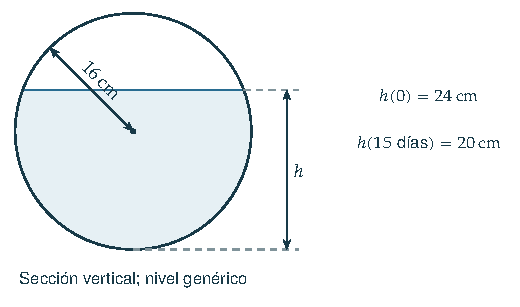
\includegraphics[width=9.86cm]{assets/M2-E0032-setup.pdf}\par
\smallskip{\small Sección del recipiente y referencia para medir la altura de agua.\par}
\end{minipage}
\end{center}

\supportlinks{M2-E0032}{1}{0}
\exercise{M2-E0101}{Core · Intermedio}
Halle una ecuación diferencial de primer orden que satisfagan todas las rectas tangentes a la parábola $y=x^2$, eliminando el parámetro del punto de tangencia.

\supportlinks{M2-E0101}{0}{0}
\exercise{M2-E0114}{Core · Intermedio}
Un tanque cilíndrico inicialmente lleno tiene radio $8\,\mathrm{dm}$ y altura $1\,\mathrm m$. Se vacía por un orificio circular de radio $1/12\,\mathrm{dm}$ situado en el fondo. La velocidad de salida suministrada es $v=0.48\sqrt h\ \mathrm{m/s}$ cuando el valor numérico de la altura $h$ se expresa en metros. Despreciando otras entradas y salidas, calcule el tiempo de vaciado.

\supportlinks{M2-E0114}{0}{0}
\exercise{M2-E0147}{Core · Básico}
Obtenga una ecuación diferencial asociada a las circunferencias no degeneradas que pasan por el origen y tienen el centro en el eje $y$, trabajando en arcos diferenciables $y(x)$.

\supportlinks{M2-E0147}{0}{0}
\exercise{M2-E0112}{Core · Intermedio}
Una roca contiene actualmente $100\,\mathrm{mg}$ de uranio y $14\,\mathrm{mg}$ de plomo procedentes de su desintegración. Use la vida media suministrada $4.5\times10^9$ años y la equivalencia: la desintegración de $238\,\mathrm{mg}$ de uranio produce $206\,\mathrm{mg}$ de plomo. Suponga que la roca inicialmente no contenía plomo, que permaneció cerrada al intercambio de ambos elementos y que se pueden despreciar los productos intermedios. Estime su edad según este modelo.

\supportlinks{M2-E0112}{0}{0}
\exercise{M2-E0146}{Core · Intermedio}
Obtenga una ecuación diferencial para los arcos diferenciables de circunferencias de radio unidad cuyo centro está en la bisectriz del segundo cuadrante. Conserve la restricción geométrica del centro al interpretar la ecuación obtenida.

\supportlinks{M2-E0146}{0}{0}
\exercise{M2-E0113}{Core · Intermedio}
En una reacción irreversible $A+B\longrightarrow C$, las cantidades se miden en unidades molares compatibles con la proporción $1:1:1$. Inicialmente $A(0)=10$, $B(0)=20$ y $C(0)=0$. El recipiente está cerrado, el volumen es constante y la velocidad de formación de $C$ es $kAB$, con $k>0$.

\begin{enumerate}[label=(\alph*),ref=\alph*,leftmargin=*]
\item Determine $k$ si a los $30$ minutos ha desaparecido el $90\%$ de $A$.
\item Determine la cantidad de producto $C(t)$ y su comportamiento mientras transcurre la reacción.
\end{enumerate}

\supportlinks{M2-E0113}{0}{0}
\exercise{M2-E0321}{Core · Intermedio}
En un ensayo idealizado, un rotor de momento de inercia \(J=2\,\mathrm{kg\,m^2}\) gira inicialmente a \(3\,\mathrm{rad/s}\). Al desconectar el motor, el único par que actúa es el de un freno viscoso: se opone al giro y vale \(-b\omega\), donde \(\omega\) es la velocidad angular y \(b=0.5\,\mathrm{N\,m\,s}\). El cambio del momento angular \(J\omega\) por unidad de tiempo es igual al par total. Se desprecia cualquier rozamiento adicional.

Tome como origen angular la posición del rotor al desconectar el motor y formule un modelo que permita saber qué ángulo recorre. Hay tres marcas situadas a \(8\), \(12\) y \(15\) radianes por delante de esa posición, contando vueltas completas. Determine cuáles alcanza y en qué instante cuando proceda. Dé después un criterio para una marca situada a un ángulo cualquiera \(\Theta>0\), y explique si la velocidad angular se anula en un tiempo finito.

\supportlinks{M2-E0321}{0}{0}
\Needspace{12\baselineskip}
\section{Problemas de síntesis}
\exercise{M2-E0141}{Core · Intermedio}
En cada apartado se propone una representación de una función o de una curva y una EDO. Decide si representa una solución real en todo el dominio indicado. Si hay que restringir el dominio o separar ramas, indica los intervalos abiertos máximos en los que se obtiene una solución. Justifica cada decisión mediante derivación y comprueba la regularidad necesaria; una igualdad que sólo se cumple en puntos aislados no basta.
\begin{enumerate}
\item $y=\ln(1+x^2)$, $x\in\mathbb{R}$; \quad $(1+x^2)y'=2x$.
\item $y=\dfrac{x}{1+x^2}$, $x\in\mathbb{R}$; \quad $(1+x^2)y'=1$.
\item $y=|x|$, $x\in\mathbb{R}$; \quad $(y')^2=1$.
\item $y^3+y=x+\sin x$, con $x,y\in\mathbb{R}$; \quad $(1+3y^2)y'=1+\cos x$. Justifica también si la relación determina una única función de $x$.
\item $y^2=\ln(1+x)$, con $x>-1$; \quad $2(1+x)yy'=1$.
\item $x=t+t^3$, $y=t^2$, $t\in\mathbb{R}$; \quad $(1+3y)^2(y')^2=4y$.
\item $x=t^3$, $y=t^6+t^3$, $t\in\mathbb{R}$; \quad $y'=2x+1$. Examina expresamente qué ocurre en $t=0$.
\end{enumerate}

\supportlinks{M2-E0141}{0}{0}
\exercise{M2-E0211}{Core · Intermedio}
Se introduce una persona infectada en una comunidad de $100$ personas susceptibles. La tasa de nuevos infectados es proporcional al producto de los infectados y los susceptibles, con coeficiente numérico $k=0.005$. Formule y resuelva el modelo de contacto. Determine cuándo se infecta la mitad del total y cuándo se alcanza el $90\%$.

Se supone comunidad cerrada, contacto homogéneo y ausencia de recuperación durante el intervalo estudiado. El tiempo se mide en la unidad usada para dar $k$; su unidad es (persona$\cdot$unidad de tiempo)$^{-1}$.

\supportlinks{M2-E0211}{0}{0}
\exercise{M2-E0182}{Core · Intermedio}
Resuelva $y'-y(y+1)/[x(x-1)]=0$. Indique las soluciones excluidas durante la separación y los intervalos de validez.

\supportlinks{M2-E0182}{0}{0}
\exercise{M2-E0144}{Core · Intermedio}
Obtenga una ecuación diferencial que satisfaga cada familia, eliminando sus parámetros constantes. Trabaje en ramas diferenciables y conserve las restricciones de las expresiones. En el cuarto apartado $\alpha\ne0$.

\begin{enumerate}[label=(\alph*),ref=\alph*,leftmargin=*]
\item $Cy^2+4y=2x^2$.
\item $y=C_1+C_2\ln x$.
\item $y=C_1+C_2e^x+C_3xe^x$.
\item $y=\alpha(\beta-e^{-x/\alpha})$, con $\alpha\ne0$.
\end{enumerate}

\supportlinks{M2-E0144}{0}{0}
\exercise{M2-E0191}{Core · Intermedio}
Discuta la existencia y unicidad de soluciones reales de $y'=\sqrt[3]{y}$, $y(0)=0$, y describa todas las soluciones definidas en $\mathbb R$.

\supportlinks{M2-E0191}{1}{0}
\exercise{M2-E0130}{Core · Intermedio}
Un objeto de masa $m>0$ se deja caer desde el reposo a una altura $H>0$. Durante el descenso, la resistencia aerodinámica es opuesta al movimiento y tiene módulo $kv^2$, con $k>0$; tome $g>0$ constante y desprecie otros efectos.

\begin{enumerate}[label=(\alph*),ref=\alph*,leftmargin=*]
\item Calcule su velocidad descendente antes del impacto.
\item Determine el tiempo hasta alcanzar el suelo.
\end{enumerate}

\supportlinks{M2-E0130}{0}{0}
\exercise{M2-E0193}{Core · Intermedio}
Resuelva $x^2y'=1-x^2+y^2-x^2y^2$, $y(1)=0$, e indique el intervalo máximo de la solución que contiene $1$.

\supportlinks{M2-E0193}{0}{0}
\exercise{M2-E0142}{Core · Intermedio}
Comprueba las siguientes afirmaciones sobre familias y parametrizaciones de soluciones. En cada caso, sustituye en la EDO y corrige la afirmación con precisión. La letra $C$ designa una constante real; en el último apartado, $t$ es el parámetro que recorre la curva. No hace falta resolver las EDO desde el principio.
\begin{enumerate}
\item «Para todo $C$, la función $y_C(x)=\tan(x+C)$ es solución de $y'=1+y^2$ en $\mathbb{R}$». Indica los intervalos abiertos máximos de cada miembro.
\item «La familia $y_C(x)=C^2(2+\sin x)$ contiene todas las soluciones de $(2+\sin x)y'=y\cos x$ y representa una sola vez cada dato inicial $y(0)=a$». Decide qué valores de $a$ admite y corrige la parametrización de la constante.
\item «Todas las funciones $y_C(x)=\ln(e^x+C)$ son soluciones de $y'=1-e^{-y}$ en su dominio real». Determina ese dominio según $C$ y averigua qué valores de $C$ hacen verdadera la sustitución.
\item «Al variar $C$, la familia $y_C(x)=Ce^{-x^2}$ recoge todas las soluciones de
\[
y''+4xy'+(4x^2+2)y=0
\]
». Verifica los miembros y contrasta la afirmación con la función $z(x)=xe^{-x^2}$, en $\mathbb{R}$.
\item «La parametrización $x=e^t$, $y=C-e^{-t}$, $t\in\mathbb{R}$, permite representar las soluciones de $x^2y'=1$ tanto para $x>0$ como para $x<0$». Comprueba qué intervalo de $x$ recorre y, si falta una componente del dominio, da una parametrización que la recorra.
\end{enumerate}

\supportlinks{M2-E0142}{0}{0}
\Needspace{12\baselineskip}
\section{Alcance y límites de una respuesta}
\exercise{M2-E0195}{Core · Intermedio}
Discuta la unicidad del PVI $y'=2\sqrt{|y|}$, $y(0)=0$, y describa sus soluciones reales globales.

\supportlinks{M2-E0195}{0}{0}
\exercise{M2-E0145}{Core · Intermedio}
Obtenga una ecuación diferencial que satisfagan los arcos representables como $y=y(x)$ de las circunferencias que pasan por el origen. Elimine los parámetros del centro y trabaje en arcos dos veces diferenciables.

\supportlinks{M2-E0145}{0}{0}
\exercise{M2-E0102}{Core · Avanzado}
Resuelva para funciones reales de clase $C^1$ la ecuación $y^{\prime}=(x-3)(y+1)^{2/3}$, donde $u^{2/3}=(\sqrt[3]{u})^2$. Incluya las soluciones que se pierdan al separar variables.

\supportlinks{M2-E0102}{0}{0}
\exercise{M2-E0368}{Core · Intermedio}
Para planificar una estación de acabado se aproxima el número de piezas pendientes de completar por una cantidad continua. Al inicio hay \(12\) piezas pendientes y llegan \(6\) piezas por minuto. La capacidad nominal es de \(10\) piezas por minuto cuando hay trabajo suficiente. No se conocen los tiempos individuales ni cómo cambia el caudal real cuando quedan pocas piezas. Los números son sintéticos.

Construya un modelo para decidir si la estación llega a quedarse sin trabajo durante los primeros diez minutos. Defina qué incluye su estado, complete las hipótesis que faltan y resuelva el modelo elegido. Explique qué hará su modelo si el estado llega a cero. Valore si la capacidad nominal basta para asegurar su conclusión y describa una observación de planta que resolvería la incertidumbre principal.

\supportlinks{M2-E0368}{0}{1}
\chapter{Balances y estructura de las EDO de primer orden}
\label{chapter:2}
%
\subsection*{Ecuación lineal y respuesta a una entrada}
\label{CH02-B01}
En un intervalo donde pueda escribirse $y'+p(t)y=q(t)$, con $p,q$
continuas, el factor integrante convierte el miembro izquierdo en una
derivada de producto. Con
$P(t)=\int_{t_0}^{t}p(s)\,ds$, el PVI tiene la representación
\[
 y(t)=e^{-P(t)}\left[y_0+\int_{t_0}^{t}e^{P(s)}q(s)\,ds\right].
\]
Así se separan la contribución del dato inicial y la de la entrada, aunque
no haya primitivas elementales. La regla del producto y el teorema
fundamental del cálculo permiten verificarla. Si antes se ha dividido por
el coeficiente de $y'$, sus ceros se estudian en la ecuación original;
el factor integrante no amplía su dominio.
Consultas: soluciones de \exref{M2-E0196} y \exref{M2-E0232}.

%
\subsection*{Exactitud, potencial y factor integrante}
\label{CH02-B02}
Al derivar parcialmente se mantiene fija la otra variable. El diferencial
de $\Phi(x,y)$ es $d\Phi=\Phi_x\,dx+\Phi_y\,dy$. Para
$M\,dx+N\,dy=0$, con $M,N$ de clase $C^1$ en un rectángulo, la igualdad
$M_y=N_x$ permite buscar $\Phi_x=M$, $\Phi_y=N$ y escribir
$\Phi=C$. Al integrar respecto de $x$, la constante es una función de $y$.
Si $\Phi_y\ne0$, el nivel define localmente un gráfico $y(x)$.

Donde los cocientes estén definidos, se pueden ensayar
\[
 \frac{\mu'(x)}{\mu(x)}=\frac{M_y-N_x}{N},\qquad
 \frac{\mu'(y)}{\mu(y)}=\frac{N_x-M_y}{M},
\]
si cada miembro derecho depende sólo de la variable indicada.
Para un factor $\mu(z(x,y))$, la regla de la cadena exige
$\mu'(z)(M z_y-N z_x)=\mu(z)(N_x-M_y)$.
Trabájese donde el factor esté definido y sea no nulo; revísense los
valores excluidos. Un ángulo definido por arctangente requiere una rama
local. La exactitud local no prueba por sí sola exactitud global en un
dominio con huecos. Consulta: solución de \exref{M2-E0021}.

%
\subsection*{Sustituciones y soluciones recuperadas}
\label{CH02-B03}
Derívese primero la variable nueva. Si $z=ax+by+c$, entonces
$z'=a+by'$; si $y=xv$, entonces $y'=v+xv'$ y se trabaja con $x\ne0$.
La ecuación de Bernoulli
\[
 y'+py=qy^n,\qquad z=y^{1-n},\qquad
 z'+(1-n)pz=(1-n)q
\]
se reduce así cuando $n\ne0,1$ y las potencias y divisiones son válidas.
Los casos $n=0,1$ son lineales. Al invertir el cambio, deben recuperarse
signos, ramas y posibles soluciones nulas de la ecuación original.
Una raíz continua no garantiza una solución derivable.

En trayectorias ortogonales, dos pendientes finitas satisfacen
$m_1m_2=-1$; una tangente horizontal corresponde a una vertical, que no se
describe mediante una pendiente finita. Recuérdense la regla de la cadena
y el dominio de las potencias reales. Consultas: soluciones de
\exref{M2-E0019} y \exref{M2-E0207}.

%
\subsection*{Balances por fases y parámetros}
\label{CH02-B04}
En una mezcla homogénea, cantidad de soluto y concentración cumplen
$Q=Vc$. Por tanto, $Q'=Vc'+V'c$: sólo con volumen constante puede
sustituirse $Q'$ por $Vc'$. Un caudal volumétrico multiplicado por una
concentración es una tasa de transporte de soluto. En balances eléctricos
o energéticos, utilícese la ley suministrada y compruébense las dimensiones
de cada constante.

Si una operación cambia en $t=a$ sin aporte instantáneo, el estado
almacenado es continuo y su valor final inicia la fase siguiente; su
derivada puede saltar. Distinguir las fases evita imponer condiciones
incompatibles. Para identificar parámetros hacen falta datos
independientes suficientes. Tratar un reactivo como constante exige que
su variación sea despreciable en el intervalo estudiado, no sólo que
inicialmente sea abundante. Consulta: solución de \exref{M2-E0030}.

\Needspace{12\baselineskip}
\section{Estructura lineal y primeros balances}
\exercise{M2-E0196}{Core · Básico}
Resuelva $y'+4y=e^{-x}$, $y(0)=4/3$.

\supportlinks{M2-E0196}{1}{0}
\exercise{M2-E0026}{Core · Básico}
Una galería de dimensiones $150\times50\times12\,\mathrm{dm}$ contiene inicialmente aire con un $0.2\%$ de $\mathrm{CO}_2$. Se introduce aire exterior con un $0.05\%$ a $9000\,\mathrm{dm^3/min}$ y se extrae el mismo caudal. Suponga mezcla uniforme, volumen constante y ausencia de otras fuentes de $\mathrm{CO}_2$. Formule el balance y determine el porcentaje al cabo de $20$ minutos.

\supportlinks{M2-E0026}{0}{0}
\exercise{M2-E0197}{Core · Básico}
Resuelva $y'+2xy=e^{x-x^2}$, $y(0)=-1$.

\supportlinks{M2-E0197}{0}{0}
\exercise{M2-E0156}{Core · Básico}
Considere $y'+y\tan x=1/\cos x$ en un intervalo con $\cos x\ne0$.

\begin{enumerate}[label=(\alph*),ref=\alph*,leftmargin=*]
\item Resuélvala mediante la fórmula general para una ecuación lineal de primer orden.
\item Resuelva primero la homogénea y aplique variación de la constante.
\end{enumerate}

\supportlinks{M2-E0156}{0}{0}
\exercise{M2-E0028}{Core · Intermedio}
Un motor genera una potencia calorífica constante $q>0$, en $\mathrm{kcal/s}$. Su masa es $m>0$ gramos y su calor específico es $\gamma>0$, en $\mathrm{kcal/(g\,{}^\circ C)}$. La refrigeración extrae una potencia $K(T-T_a)$, con $K>0$ en $\mathrm{kcal/(s\,{}^\circ C)}$ y temperatura ambiente constante $T_a$. Suponga temperatura uniforme y parámetros constantes, con $T(0)=T_a$.

\begin{enumerate}[label=(\alph*),ref=\alph*,leftmargin=*]
\item Formule el balance y determine $T(t)$.
\item Halle la temperatura de régimen y determine si se alcanza en un tiempo finito.
\end{enumerate}

\supportlinks{M2-E0028}{0}{0}
\exercise{M2-E0167}{Core · Básico}
Resuelva $y^{\prime}-y\tan x=-1$, sabiendo que admite un factor integrante dependiente sólo de $x$.

\supportlinks{M2-E0167}{0}{0}
\exercise{M2-E0247}{Core · Intermedio}
Una población se modela mediante $P'=kP+r$, $P(0)=P_0$, con $r>0$, $P_0\ge0$ y $k\in\mathbb R$. Resuelva el modelo y analice según el signo de $k$ el comportamiento a largo plazo, el equilibrio físico y la posibilidad de extinción.

\supportlinks{M2-E0247}{0}{0}
\exercise{M2-E0020}{Core · Básico}
Resuelva $y^{\prime}=\dfrac{-2x-y}{x-1}$, $y(0)=1$, e indique el intervalo máximo que contiene el dato inicial.

\supportlinks{M2-E0020}{0}{0}
\exercise{M2-E0187}{Core · Básico}
Resuelva las ecuaciones siguientes e indique sus dominios de definición.

\begin{enumerate}[label=(\alph*),ref=\alph*,leftmargin=*]
\item $y^{\prime}+y=1/(1+e^{2x})$.
\item $y^{\prime}+y=2xe^{-x}+x^2$.
\item $y-x+xy\cot x+xy^{\prime}=0$.
\end{enumerate}

\supportlinks{M2-E0187}{0}{0}
\Needspace{12\baselineskip}
\section{Formas diferenciales y soluciones implícitas}
\exercise{M2-E0220}{Core · Básico}
Resuelva $2xy\,dx+(x^2-1)\,dy=0$ para funciones reales $y(x)$.

\supportlinks{M2-E0220}{0}{0}
\exercise{M2-E0018}{Core · Básico}
Considere la ecuación $(y-x)\,dx+x\,dy=0$ para funciones reales $y(x)$.

\begin{enumerate}[label=(\alph*),ref=\alph*,leftmargin=*]
\item Clasifíquela por orden y linealidad e identifique las estructuras que permiten resolverla. Especifique las restricciones de cada forma.
\item Resuélvala por las estructuras anteriores y compare los resultados. Determine qué soluciones pueden atravesar $x=0$.
\end{enumerate}

\supportlinks{M2-E0018}{0}{0}
\exercise{M2-E0221}{Core · Básico}
Resuelva implícitamente la forma diferencial
\[[e^{2y}-y\cos(xy)]\,dx+[2xe^{2y}-x\cos(xy)+2y]\,dy=0.\]
Indique dónde la relación define localmente un gráfico $y(x)$.

\supportlinks{M2-E0221}{0}{0}
\exercise{M2-E0205}{Core · Intermedio}
Trabaje con funciones continuas $f$ y $g$ en las regiones consideradas.

\begin{enumerate}[label=(\alph*),ref=\alph*,leftmargin=*]
\item Muestre que una ecuación separable $y^{\prime}=f(x)g(y)$ puede escribirse como una ecuación exacta en cada región donde $g(y)\ne0$. Indique cómo tratar los ceros de $g$.
\item Use este procedimiento para escribir $y^{\prime}=xy$ como ecuación exacta y resolverla.
\end{enumerate}

\supportlinks{M2-E0205}{0}{0}
\exercise{M2-E0021}{Core · Intermedio}
Resuelva $y^2+(xy+1)y^{\prime}=0$. Si usa un factor integrante, indique dónde es válido y compruebe las soluciones excluidas durante el cálculo.

\supportlinks{M2-E0021}{1}{0}
\exercise{M2-E0204}{Core · Básico}
Encuentre un factor integrante no nulo para cada forma diferencial, en las regiones de su dominio, y compruebe la exactitud.

\begin{enumerate}[label=(\alph*),ref=\alph*,leftmargin=*]
\item $y^{-1}\,dx+3y\,dy=0$.
\item $dx-e^{-x-y}\,dy=0$.
\item $\left(\cos x/y^2+1/y\right)\,dx+(x/y^2)\,dy=0$.
\item $\left(2y+y^2/x\right)\,dx+(2y+x)\,dy=0$.
\end{enumerate}

\supportlinks{M2-E0204}{0}{0}
\exercise{M2-E0234}{Core · Intermedio}
Resuelva $xy\,dx+(2x^2+3y^2-20)\,dy=0$ mediante un factor integrante que dependa de $y$. Compruebe las soluciones excluidas por dicho factor.

\supportlinks{M2-E0234}{0}{0}
\exercise{M2-E0131}{Core · Intermedio}
Resuelva los siguientes problemas de valor inicial para funciones reales. Describa la rama que contiene el dato inicial.

\begin{enumerate}[label=(\alph*),ref=\alph*,leftmargin=*]
\item $3x^2y^2+(2x^3y+4y^3)y^{\prime}=0$, $y(1)=-1$.
\item $y+2xy^3+(1+3x^2y^2+x)y^{\prime}=0$, $y(-1)=1$.
\end{enumerate}

\supportlinks{M2-E0131}{0}{0}
\exercise{M2-E0250}{Core · Intermedio}
Resuelva $(2y^2+3x)\,dx+2xy\,dy=0$ para gráficos reales y examine los puntos que se excluyen al usar un factor integrante.

\supportlinks{M2-E0250}{0}{0}
\exercise{M2-E0133}{Core · Intermedio}
Resuelva $(3y^2-x)\,dx+(2y^3-6xy)\,dy=0$, sabiendo que admite un factor integrante de la forma $f(x+y^2)$. Compruebe las curvas excluidas por ese factor.

\supportlinks{M2-E0133}{0}{0}
\Needspace{12\baselineskip}
\section{Cambios de variable y recuperación de ramas}
\exercise{M2-E0019}{Core · Intermedio}
Resuelva las siguientes ecuaciones para funciones reales e indique los intervalos de validez. Compruebe las soluciones que puedan perderse al dividir.

\begin{enumerate}[label=(\alph*),ref=\alph*,leftmargin=*]
\item $y^{\prime}=(x-y)^2$.
\item $y^{\prime}=(y+x)/x$.
\item $e^{-y}(1+y^{\prime})=1$.
\end{enumerate}

\supportlinks{M2-E0019}{1}{0}
\exercise{M2-E0104}{Core · Intermedio}
Resuelva $y^{\prime}=1/(x+y+1)$ e indique las restricciones de las ramas obtenidas.

\supportlinks{M2-E0104}{0}{0}
\exercise{M2-E0207}{Core · Intermedio}
Resuelva $y'-5y=-(5/2)xy^3$ para funciones reales y recupere cualquier solución excluida por la transformación.

\supportlinks{M2-E0207}{1}{0}
\exercise{M2-E0185}{Core · Intermedio}
Resuelva estas ecuaciones, especificando las restricciones de las ramas reales y comprobando las soluciones excluidas por los cambios de variable.

\begin{enumerate}[label=(\alph*),ref=\alph*,leftmargin=*]
\item $xy^{\prime}+y=1/y^2$.
\item $y^{\prime}=y(xy^3-1)$.
\end{enumerate}

\supportlinks{M2-E0185}{0}{0}
\exercise{M2-E0111}{Core · Intermedio}
Resuelva $2x+2y-1+(x+y-2)y^{\prime}=0$ e indique las restricciones de las ramas gráficas.

\supportlinks{M2-E0111}{0}{0}
\exercise{M2-E0105}{Core · Intermedio}
Resuelva $(x+y)^2y^{\prime}=a^2$ para $a\in\mathbb R$, incluyendo el caso $a=0$. Indique dónde son válidas las soluciones reales.

\supportlinks{M2-E0105}{0}{0}
\exercise{M2-E0164}{Core · Intermedio}
Resuelva el PVI $y^{\prime}=2xy/(y^2-x^2)$, $y(0)=1$, indicando la rama real que corresponde al dato y su dominio.

\supportlinks{M2-E0164}{0}{0}
\exercise{M2-E0149}{Core · Intermedio}
Resuelva las siguientes ecuaciones, conservando los dominios y comprobando las soluciones excluidas por las divisiones. En una forma diferencial se entiende $dy=y^{\prime}dx$.

\begin{enumerate}[label=(\alph*),ref=\alph*,leftmargin=*]
\item $(x^2-xy-y^2)\,dx-xy\,dy=0$.
\item $(2x+y+1)\,dx+(4x+2y+3)\,dy=0$.
\end{enumerate}

\supportlinks{M2-E0149}{0}{0}
\exercise{M2-E0210}{Core · Intermedio}
Resuelva $xy'+(x+1)y+xy^5=0$, $y(1)=1$, en el intervalo máximo que contiene el dato. Se admite una respuesta por cuadratura.

\supportlinks{M2-E0210}{0}{0}
\exercise{M2-E0148}{Core · Avanzado}
Resuelva las ecuaciones siguientes para funciones reales de clase $C^1$. Conserve las restricciones de las expresiones y las ramas que puedan perderse al separar variables.

\begin{enumerate}[label=(\alph*),ref=\alph*,leftmargin=*]
\item $y^{\prime}=(y^2+2xy)/(x^2+2xy)$.
\item $xy^{\prime}=y+\sqrt{y^2-x^2}$, con la raíz real no negativa.
\end{enumerate}

\supportlinks{M2-E0148}{0}{0}
\Needspace{12\baselineskip}
\section{Balances, entradas y condiciones}
\exercise{M2-E0218}{Core · Básico}
Un depósito de sección horizontal constante tiene altura total $3\,\mathrm m$ y un orificio circular de radio $0.05\,\mathrm m$ en el fondo. La velocidad de salida es $c\sqrt{2gh}$, donde $h$ es la altura de agua, $0<c<1$ y $g=9.8\,\mathrm{m/s^2}$. Determine la EDO para $h$, denotando por $A_w$ el área horizontal del depósito.

Se supone líquido incompresible, superficie horizontal, sección constante $A_w>0$, orificio pequeño y velocidad de salida suministrada por la ley indicada. Se aplica el modelo mientras queda agua y no se excede la altura del depósito.

\supportlinks{M2-E0218}{0}{0}
\exercise{M2-E0232}{Core · Intermedio}
Considere un circuito ideal en serie con inductancia $L>0$, resistencia $R>0$, tensión aplicada $E(t)$ y corriente $I(t)$.

Los componentes son ideales, L y R son constantes positivas y se desprecia cualquier capacitancia. La orientación de corriente es la del generador. En (a) la tensión es constante y t=0 es el cierre; en (b) E es continua en el intervalo de tiempo considerado y puede variar.

\begin{enumerate}[label=(\alph*),ref=\alph*,leftmargin=*]
\item Una batería de $12\,\mathrm V$ se conecta a un circuito con $L=0.5\,\mathrm H$ y $R=10\,\Omega$. La corriente inicial es cero. Determine la corriente después de cerrar el circuito.
\item Para una tensión continua $E(t)$, compruebe que la solución general de $LI^{\prime}+RI=E(t)$ puede escribirse como \[I(t)=e^{-Rt/L}\left[C+\frac1L\int_0^t e^{Rs/L}E(s)\,ds\right].\] Especialice la fórmula a $E(t)=E_0$ constante e identifique el término transitorio y la corriente de régimen.
\end{enumerate}

\supportlinks{M2-E0232}{1}{0}
\exercise{M2-E0219}{Core · Intermedio}
Un depósito es un cono circular invertido, de altura $6\,\mathrm m$ y radio superior $2.5\,\mathrm m$. El agua sale por un orificio circular de radio $0.02\,\mathrm m$ en el vértice inferior, con velocidad $0.6\sqrt{2gh}$, $g=9.8\,\mathrm{m/s^2}$. Determine la EDO para la altura de agua $h$.

Se supone líquido incompresible, salida única por el orificio, geometría cónica ideal y ley de salida suministrada. La EDO para la altura se usa mientras $h>0$; su coeficiente singular al agotarse el agua impide aplicarla literalmente en $h=0$.

\Needspace{11.28cm}
\begin{center}
\begin{minipage}{\linewidth}
\centering
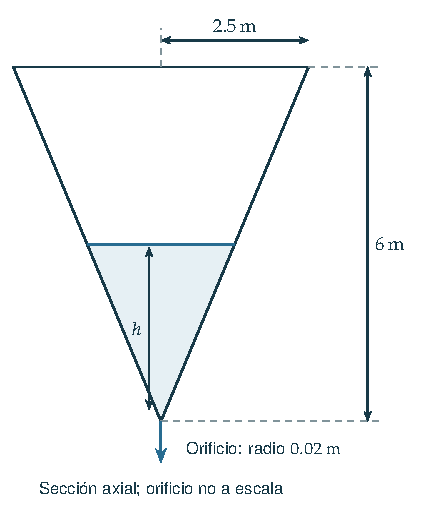
\includegraphics[width=8.03cm]{assets/M2-E0219-setup.pdf}\par
\smallskip{\small Geometría del depósito cónico y referencia de la altura de agua.\par}
\end{minipage}
\end{center}

\supportlinks{M2-E0219}{0}{0}
\exercise{M2-E0022}{Core · Intermedio}
La temperatura $T(t)$ de un cuerpo obedece $T^{\prime}=-k[T-A(t)]$, con $k>0$ y $A(t)=A_0\cos(\omega t)$. Las temperaturas se expresan respecto del mismo origen; $k$ y $\omega$ tienen unidades de tiempo inverso y $A_0$ tiene unidades de temperatura.

\begin{enumerate}[label=(\alph*),ref=\alph*,leftmargin=*]
\item Halle la solución general.
\item Explique cómo influye la condición inicial a largo plazo.
\end{enumerate}

\supportlinks{M2-E0022}{0}{0}
\exercise{M2-E0029}{Core · Intermedio}
Un depósito contiene inicialmente $40\,\mathrm L$ de agua pura. En el modelo de mezcla se introduce una disolución con concentración suministrada de $3\,\mathrm{kg/L}$ a $2\,\mathrm{L/min}$ y sale mezcla homogénea a $3\,\mathrm{L/min}$. Suponga volúmenes aditivos y mezcla perfecta. Use $t=0$ al comenzar ambos flujos y limite el modelo al tiempo anterior al vaciado.

\begin{enumerate}[label=(\alph*),ref=\alph*,leftmargin=*]
\item Determine la cantidad de sal $S(t)$.
\item Calcule la cantidad cuando quedan $20\,\mathrm L$.
\item Determine cuándo es máxima la cantidad de sal.
\end{enumerate}

\supportlinks{M2-E0029}{0}{0}
\exercise{M2-E0031}{Core · Intermedio}
Un tanque de $100\,\mathrm L$ contiene inicialmente $50\,\mathrm L$ de agua pura. Entra disolución de $0.1\,\mathrm{kg/L}$ a $4\,\mathrm{L/min}$ y sale mezcla a $2\,\mathrm{L/min}$ por una tubería. Cuando el tanque se llena, el exceso sale por un rebosadero. Suponga mezcla perfecta y volúmenes aditivos. Formule los balances de cada régimen y determine la cantidad de sal $S(t)$ para $t\ge0$.

\Needspace{5.61cm}
\begin{center}
\begin{minipage}{\linewidth}
\centering
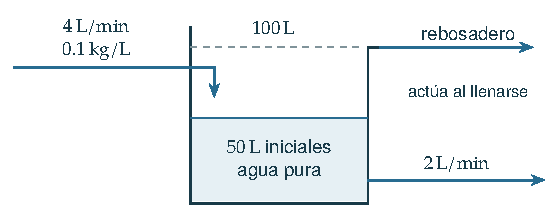
\includegraphics[width=10.59cm]{assets/M2-E0031-setup.pdf}\par
\smallskip{\small Tubería de salida y rebosadero del depósito.\par}
\end{minipage}
\end{center}

\supportlinks{M2-E0031}{0}{0}
\exercise{M2-E0317}{Core · Básico}
En un ensayo simulado, un depósito de capacidad \(80\,\mathrm L\) contiene inicialmente \(50\,\mathrm L\) de agua limpia. Entran \(3\,\mathrm{L/min}\) de agua limpia y sale \(1\,\mathrm{L/min}\) de mezcla. El contenido se mantiene uniforme y el soluto no reacciona ni se pierde por otros mecanismos. Un dosificador añade soluto sin aportar un volumen apreciable; puede suministrar entre \(0\) y \(2\,\mathrm{g/min}\).

Se desea que la concentración siga la ley \(c(t)=0.02t\,\mathrm{g/L}\), donde \(t\) es el valor numérico del tiempo transcurrido en minutos. Elija las cantidades necesarias para describir el proceso y formule sus balances. Determine cómo debe variar el suministro del dosificador y durante cuánto tiempo puede mantenerse la concentración solicitada, respetando tanto la capacidad del depósito como la del dosificador. Indique cuál de las dos limita primero la operación.

\supportlinks{M2-E0317}{0}{0}
\Needspace{12\baselineskip}
\section{Problemas de elección y comprobación}
\exercise{M2-E0138}{Core · Intermedio}
Clasifique las siguientes EDO de primer orden. Indique las estructuras aplicables y sus restricciones, justificando la clasificación sin necesidad de resolverlas.

\begin{enumerate}[label=(\alph*),ref=\alph*,leftmargin=*]
\item $x(x^3+1)y^{\prime}+(2x^3-1)y=(x^3-2)/x$.
\item $y^{\prime}=a\cos(x-y+2)$, $a\in\mathbb R$.
\item $(3x^2+6xy^2)\,dx+(6x^2y+4y^3)\,dy=0$.
\item $y^{\prime}+2y=x$.
\item $yy^{\prime}=2\sqrt{xy}-x$.
\item $(1+y^2)\,dx=xy\,dy$.
\item $(x+3y)\,dx+(3x+9y+2)\,dy=0$.
\item $e^x\tan y\,dx+2\sin^2y\,dy=0$.
\item $2xyy^{\prime}=3x^2-y^2$.
\end{enumerate}

\supportlinks{M2-E0138}{0}{0}
\exercise{M2-E0364}{Core · Intermedio}
Sea \(\alpha\in\mathbb R\). Para \(x>0\), considere
\[
\bigl((2+\alpha)xy+1\bigr)\,dx+x^2\,dy=0.
\]
Clasifique la ecuación y elija una estrategia antes de resolverla. Obtenga todas las soluciones reales para cada valor de \(\alpha\), justificando los casos que deban tratarse por separado. Compare dos vías de resolución en un caso que usted elija y explique cuál prefiere. Compruebe las soluciones que puedan perderse al dividir durante sus cálculos.

\supportlinks{M2-E0364}{0}{0}
\exercise{M2-E0184}{Core · Intermedio}
Resuelva las ecuaciones siguientes, conservando el dominio de cada expresión original. En los PVI indique el intervalo máximo que contiene el dato.

\begin{enumerate}[label=(\alph*),ref=\alph*,leftmargin=*]
\item $xy^{\prime}+(2x+1)y=xe^{-2x}$.
\item $y^{\prime}=2y/(x+1)+(x+1)^3$, $y(0)=1$.
\item $(x^2+1)y^{\prime}+3xy=6x$, $y(0)=1$.
\item $xy^{\prime}+\dfrac{2x+1}{x+1}y=x-1$.
\end{enumerate}

\supportlinks{M2-E0184}{0}{0}
\exercise{M2-E0163}{Core · Intermedio}
Determine las trayectorias ortogonales a la familia de curvas $y=x+Ce^{-x}$, $C\in\mathbb R$.

\supportlinks{M2-E0163}{0}{0}
\exercise{M2-E0363}{Core · Intermedio}
Compare las ecuaciones, con variables adimensionales,
\[
\mathrm A:\quad y'+(1+t)y=t,
\qquad
\mathrm B:\quad y'+(1+t)y=t y^2.
\]
Antes de calcular, clasifique cada una y elija una vía de resolución, explicando qué cambia de A a B. Obtenga todas sus soluciones reales; se admiten integrales definidas. Indique los intervalos donde sus expresiones son válidas y compruebe si el procedimiento excluye alguna solución.

\supportlinks{M2-E0363}{0}{1}
\exercise{M2-E0190}{Core · Intermedio}
Resuelva las siguientes ecuaciones lineales. En los apartados con dato inicial, determine la solución correspondiente.

\begin{enumerate}[label=(\alph*),ref=\alph*,leftmargin=*]
\item $y^{\prime}+xy=x$.
\item $y^{\prime}+6y=e^x$.
\item $y^{\prime}+3x^2y=\sin x\,e^{-x^3}$, $y(0)=1$.
\item $y^{\prime}+\cos x\,y=\cos x$.
\item $y^{\prime}/(1+x^2)+xy=3$, $y(0)=0$.
\item $y^{\prime}+2\sin(2x)y=2\sin(2x)$, $y(\pi/2)=3$.
\end{enumerate}

\supportlinks{M2-E0190}{0}{0}
\exercise{M2-E0175}{Core · Intermedio}
Considere $(x^2+y^2+1)\,dx-2xy\,dy=0$.

\begin{enumerate}[label=(\alph*),ref=\alph*,leftmargin=*]
\item Resuélvala usando un factor de la forma $f(y^2-x^2)$.
\item Resuélvala usando un factor de la forma $f(x)$.
\item Resuelva teniendo en cuenta ambos resultados.
\end{enumerate}

\supportlinks{M2-E0175}{0}{0}
\exercise{M2-E0249}{Core · Intermedio}
Resuelva $(-xy\sin x+2y\cos x)\,dx+2x\cos x\,dy=0$ para gráficos reales $y(x)$.

\supportlinks{M2-E0249}{0}{0}
\exercise{M2-E0202}{Core · Avanzado}
Resuelva las ecuaciones siguientes. Distinga las restricciones de la ecuación original de las divisiones introducidas por el método.

\begin{enumerate}[label=(\alph*),ref=\alph*,leftmargin=*]
\item $x^2y^{\prime}=y^2+xy$, $y(1)=1$.
\item $yy^{\prime}+x=\sqrt{x^2+y^2}$.
\item $y^{\prime}=(x^2-y^2)/(xy)$, $y(1)=2$.
\item $xy^{\prime}+y+x=0$, $y(1)=1$.
\end{enumerate}

\supportlinks{M2-E0202}{0}{0}
\exercise{M2-E0222}{Core · Intermedio}
Resuelva $y'=[xy^2-\cos x\sin x]/[y(1-x^2)]$, $y(0)=2$, e indique el intervalo máximo de esa rama.

\supportlinks{M2-E0222}{0}{0}
\Needspace{12\baselineskip}
\section{Relaciones y restricciones}
\exercise{M2-E0135}{Core · Avanzado}
Sean $P,Q$ funciones de clase $C^1$ en un rectángulo con $x>0$, $y>0$, y sean $n,m\in\mathbb R$.

\begin{enumerate}[label=(\alph*),ref=\alph*,leftmargin=*]
\item Obtenga la condición necesaria y suficiente para que $\mu=x^ny^m$ transforme $P\,dx+Q\,dy$ en una forma exacta.
\item Encuentre un factor monomial para $(2xy+y^3)\,dx+(3x^2+xy^2)\,dy=0$ e integre con él. Compruebe también la solución sobre $y=0$.
\end{enumerate}

\supportlinks{M2-E0135}{0}{0}
\exercise{M2-E0132}{Core · Intermedio}
Considere $x^2y^3+x(1+y^2)y^{\prime}=0$. Trabaje primero en regiones con $xy\ne0$ y compruebe después las soluciones excluidas.

\begin{enumerate}[label=(\alph*),ref=\alph*,leftmargin=*]
\item ¿Es exacta la forma diferencial original?
\item Busque un factor integrante de la forma $f(xy^3)$ y resuelva.
\item ¿Existe un factor integrante no nulo de la forma $f(xy)$ para la forma original en una región con $xy\ne0$?
\end{enumerate}

\supportlinks{M2-E0132}{0}{0}
\exercise{M2-E0199}{Core · Avanzado}
En un medio de volumen constante, $A+B\xrightarrow{k_1}C\xrightarrow{k_2}D$, con cinética de acción de masas, $k_1,k_2>0$. Inicialmente $A(0)=A_0$, $B(0)=B_0$, $C(0)=D(0)=0$ y $A_0\gg B_0>0$. Para las expresiones explícitas use la aproximación de reactivo en exceso $k_1A(t)\simeq k_1A_0=\lambda$, distinguiéndola de los balances de materia. Las cantidades se expresan como concentraciones compatibles con la estequiometría uno a uno.

\begin{enumerate}[label=(\alph*),ref=\alph*,leftmargin=*]
\item Dé las ecuaciones diferenciales y los balances de materia del sistema.
\item Determine las cantidades de los cuatro compuestos con el tiempo en esa aproximación.
\item Pruebe que, si $A_0=k_2/k_1$, el máximo de $C$ en el modelo reducido no depende de las constantes de reacción. Halle ese máximo y el instante en que se alcanza.
\end{enumerate}

\supportlinks{M2-E0199}{0}{0}
\exercise{M2-E0309}{Core · Intermedio}
Un ensayo simulado representa un depósito bien mezclado de \(100\,\mathrm L\). Entra agua limpia a caudal constante desconocido \(q>0\), en \(\mathrm{L/min}\), y sale mezcla al mismo caudal. Además, un proceso interno consume por minuto una fracción \(k\ge0\) de la masa de contaminante presente; \(k\) se mide en \(\mathrm{min}^{-1}\). La concentración registrada, tratada como exacta en este ejercicio, es
\[
c(t)=2e^{-0.12t}\ \mathrm{g/L},\qquad t\ge0.
\]
Formule el balance y determine todo lo que esta curva permite inferir sobre \(q\) y \(k\). Se puede repetir el ensayo sin cambiar el régimen hidráulico, añadiendo una pequeña cantidad de un trazador que no reacciona, no se adsorbe y no altera el proceso. ¿Aporta más información volver a medir el volumen constante o medir la disminución del trazador? En la repetición, la concentración del trazador se reduce a la mitad en diez minutos. Determine entonces \(q\) y \(k\), y compruebe su compatibilidad con las hipótesis.

\supportlinks{M2-E0309}{0}{0}
\exercise{M2-E0136}{Core · Avanzado}
Sea $f$ de clase $C^1$ para argumentos positivos. Considere $[y+xf(x^2+y^2)]\,dx+[yf(x^2+y^2)-x]\,dy=0$. Trabaje localmente en una región simplemente conexa que no contenga el origen, donde se pueda elegir una rama continua del ángulo.

\begin{enumerate}[label=(\alph*),ref=\alph*,leftmargin=*]
\item Pruebe que $\mu=1/(x^2+y^2)$ es un factor integrante local.
\item Resuelva con ese factor cuando $f(s)=s^2$.
\end{enumerate}

\supportlinks{M2-E0136}{0}{0}
\exercise{M2-E0168}{Core · Avanzado}
Considere $(ax^3y^4+by)\,dx+(cx^4y^3+ex)\,dy=0$, con parámetros reales. Para factores con exponentes reales trabaje en una región donde $x$ e $y$ no se anulen y conserve sus signos; se puede escribir $\mu=|x|^{\alpha}|y|^{\beta}$.

\begin{enumerate}[label=(\alph*),ref=\alph*,leftmargin=*]
\item Demuestre que existe un factor de esta forma cuando $ae-bc\ne0$ y determine los exponentes.
\item Resuelva $(2x^3y^4+3y)\,dx+(x^4y^3-3x)\,dy=0$.
\end{enumerate}

\supportlinks{M2-E0168}{0}{0}
\exercise{M2-E0173}{Core · Avanzado}
Considere $\left(x+\frac2y\right)\,dx+\left(\frac{x^2}{3y}+\frac yx\right)\,dy=0$ en una región abierta con $xy\ne0$.

\begin{enumerate}[label=(\alph*),ref=\alph*,leftmargin=*]
\item ¿Es exacta? Justifique la respuesta.
\item Decida si admite un factor de la forma $f(xy)$; en caso afirmativo, calcúlelo y resuelva.
\item Decida si admite un factor no nulo de la forma $f(x/y)$; en caso afirmativo, calcúlelo y resuelva.
\end{enumerate}

\supportlinks{M2-E0173}{0}{0}
\exercise{M2-E0172}{Core · Intermedio}
Demuestre que $y+(\sqrt{x^2+y^2}-x)y^{\prime}=0$ admite un factor integrante de la forma $\mu(x,y)=y^{-1}f(x^2+y^2)$. Hállelo y resuelva la ecuación.

\supportlinks{M2-E0172}{0}{0}
\exercise{M2-E0189}{Core · Intermedio}
Considere la familia $x^2+y^2=ay+1$, $a\in\mathbb R$.

\begin{enumerate}[label=(\alph*),ref=\alph*,leftmargin=*]
\item Determine su ecuación diferencial asociada.
\item Halle sus trayectorias ortogonales.
\end{enumerate}

\supportlinks{M2-E0189}{0}{0}
\exercise{M2-E0200}{Core · Avanzado}
Un sustrato $A$ y un catalizador $E$ forman reversiblemente el intermedio $B$: $A+E\mathrel{\mathop{\rightleftharpoons}^{k_1}_{k_2}}B\xrightarrow{k_3}C+E$. Las constantes son positivas, el volumen es constante y se aplica acción de masas. Inicialmente $A(0)=A_0$, $E(0)=E_0$, $B(0)=C(0)=0$, con $A_0\gg E_0>0$. Para la solución explícita use la aproximación $k_1A(t)\simeq k_1A_0=\lambda$ mientras el consumo de sustrato sea pequeño respecto de $A_0$.

\begin{enumerate}[label=(\alph*),ref=\alph*,leftmargin=*]
\item Dé las ecuaciones diferenciales que rigen el sistema.
\item Obtenga la relación entre las cantidades del intermedio $B$ y del catalizador $E$.
\item Determine las cantidades de los cuatro compuestos con el tiempo en el modelo reducido.
\end{enumerate}

\supportlinks{M2-E0200}{0}{0}
\exercise{M2-E0171}{Core · Avanzado}
Determine un factor integrante de la forma $\mu(x,y)=x^\alpha f(y/x)$ para $x^2y+y^3-xy+x^2y^{\prime}=0$ y resuelva con su ayuda.

\supportlinks{M2-E0171}{0}{0}
\exercise{M2-E0174}{Core · Intermedio}
Considere $y+x(x^2y-1)y^{\prime}=0$.

\begin{enumerate}[label=(\alph*),ref=\alph*,leftmargin=*]
\item Encuentre un factor integrante de la forma $\mu=y^{-2}f(x/y)$.
\item Resuelva analíticamente con su ayuda, comprobando las ramas excluidas por el factor.
\end{enumerate}

\supportlinks{M2-E0174}{0}{0}
\exercise{M2-E0139}{Core · Avanzado}
Considere $[(xy-\tan(xy))/x^2]\,dx+dy=0$, con $x\ne0$ y $\cos(xy)\ne0$.

\begin{enumerate}[label=(\alph*),ref=\alph*,leftmargin=*]
\item ¿Es exacta la forma diferencial original?
\item ¿Admite un factor integrante no nulo de la forma $f(x+y)$, con $f$ de clase $C^1$, en alguna región abierta del dominio natural? Justifique su respuesta y, en caso afirmativo, utilícelo para resolver la ecuación.
\item Busque un factor de la forma $f(xy)$ y resuelva en el dominio natural.
\end{enumerate}

\supportlinks{M2-E0139}{0}{0}
\Needspace{12\baselineskip}
\section{Regímenes y contrastes}
\exercise{M2-E0373}{Core · Intermedio · Oral · Croquis a mano}
Un módulo de alimentación carga un condensador con corriente constante \(I>0\). Se adopta el modelo
\[
C v'=I-Gv,\qquad v(0)=0,
\]
donde \(C>0\) es la capacidad y \(G>0\) la conductancia de fuga. \(v\) se mide en voltios, \(t\) en segundos, \(C\) en faradios, \(G\) en siemens e \(I\) en amperios.

Compare oralmente tres diseños: el original, otro con el doble de capacidad y otro con el doble de conductancia, manteniendo los demás valores. Prediga la pendiente inicial y la tensión límite de cada uno, y dibuje a mano las tres respuestas en los mismos ejes. Justifique qué curvas pueden cruzarse después del arranque. No es necesario localizar el cruce ni desarrollar todas las fórmulas.

\supportlinks{M2-E0373}{0}{0}
\exercise{M2-E0030}{Core · Avanzado}
Un tanque de capacidad $100\,\mathrm L$ contiene inicialmente $50\,\mathrm L$ de agua pura. Desde $t=0$ entra una disolución de $2\,\mathrm{g/L}$ a $5\,\mathrm{L/min}$. En $t=3$ minutos comienza a salir mezcla homogénea a $6\,\mathrm{L/min}$, mientras continúa la entrada. Suponga mezcla perfecta y volúmenes aditivos; el modelo de mezcla termina al vaciarse el tanque.

\begin{enumerate}[label=(\alph*),ref=\alph*,leftmargin=*]
\item Determine el volumen y la cantidad de sal en cada régimen.
\item Obtenga la concentración y explique el comportamiento al final del intervalo físico. ¿Se puede interpretar aquí un límite cuando $t\to\infty$?
\item Halle el máximo de la cantidad de sal, el instante y el volumen correspondientes.
\end{enumerate}

\Needspace{6.68cm}
\begin{center}
\begin{minipage}{\linewidth}
\centering
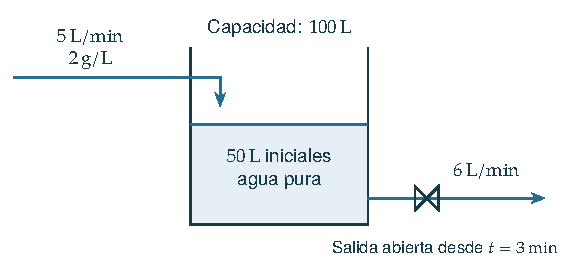
\includegraphics[width=10.94cm]{assets/M2-E0030-setup.pdf}\par
\smallskip{\small Entrada continua y apertura retardada de la salida.\par}
\end{minipage}
\end{center}

\supportlinks{M2-E0030}{1}{0}
\exercise{M2-E0023}{Core · Avanzado}
Resuelva los siguientes problemas de valor inicial. Puede expresar las soluciones mediante integrales definidas. Indique en cada caso el intervalo de validez de la rama que contiene el dato inicial.

\begin{enumerate}[label=(\alph*),ref=\alph*,leftmargin=*]
\item $y^{\prime}+(x^2-1)y+xy^6=0$, $y(1)=1$.
\item $y^{\prime}+xy=y^4$, $y(0)=1$.
\item $xy^{\prime}+y+y^2=0$, $y(1)=2$.
\end{enumerate}

\supportlinks{M2-E0023}{0}{0}
\exercise{M2-E0307}{Core · Intermedio}
En un ensayo simulado, la temperatura del proceso es \(R(t)=20+2t\), en grados Celsius, durante \(0\le t\le10\) segundos. Un sensor inicialmente a \(20\,{}^\circ\mathrm C\) tiene capacidad térmica \(C>0\). La potencia térmica que recibe del proceso es proporcional a la diferencia entre la temperatura del proceso y la temperatura del propio sensor, con coeficiente \(H>0\); \(C/H=3\,\mathrm s\). No hay otros intercambios y el sensor no altera la temperatura del proceso.

Elija las cantidades con las que describirá la medición, formule el modelo con su condición inicial y obtenga la lectura del sensor. Se admite una diferencia de, como máximo, \(4\,{}^\circ\mathrm C\) entre la lectura y la temperatura del proceso: determine durante qué parte del ensayo se cumple esa tolerancia. Si se quiere mantener una rampa durante los diez segundos, ¿cuál es la mayor pendiente constante \(a\ge0\) admisible en \(R(t)=20+at\), con el mismo estado inicial? Justifique la decisión a partir del modelo.

\supportlinks{M2-E0307}{0}{0}
\exercise{M2-E0115}{Core · Avanzado}
Una persona de masa $100\,\mathrm{kg}$ se deja caer desde $3000\,\mathrm m$, con velocidad vertical inicial nula. La resistencia del aire es proporcional a la velocidad, con coeficiente $20\,\mathrm{kg/s}$ antes de abrir el paracaídas y $100\,\mathrm{kg/s}$ después. Use $g=9.8\,\mathrm{m/s^2}$, suponga apertura instantánea sin impulso y mida los tiempos desde el inicio de la caída.

\begin{enumerate}[label=(\alph*),ref=\alph*,leftmargin=*]
\item ¿Cuándo alcanza el suelo si abre el paracaídas a los $30$ segundos?
\item ¿Cuándo alcanza el suelo si la apertura se retrasa hasta los $60$ segundos?
\end{enumerate}

\supportlinks{M2-E0115}{0}{0}
\exercise{M2-E0166}{Core · Avanzado}
Resuelva las ecuaciones siguientes. En los apartados con dato inicial, seleccione la rama que lo satisface. Las expresiones con $\log y$ requieren $y>0$.

\begin{enumerate}[label=(\alph*),ref=\alph*,leftmargin=*]
\item $(2x\cos y+3x^2y)\,dx+(x^3-x^2\sin y-y)\,dy=0$.
\item $(x+y)^2\,dx+(2xy+x^2-1)\,dy=0$, $y(1)=1$.
\item $(y^2\cos x-3x^2y-2x)\,dx+(2y\sin x-x^3+\log y)\,dy=0$, $y(0)=e$.
\item $y(2x+y^3)\,dx-x(2x-y^3)\,dy=0$.
\item $(2xy+y^3)\,dx+(2y^3-x^2+xy^2)\,dy=0$.
\end{enumerate}

\supportlinks{M2-E0166}{0}{0}
\exercise{M2-E0206}{Core · Intermedio}
Una comunidad tiene inicialmente $100$ habitantes. Su crecimiento interno es proporcional a la población, con tasa numérica $0.15(1+t^2)$, y recibe inmigración neta constante de $20$ personas al año. Use $t$ como valor numérico del tiempo en años y $P$ como población continua del modelo.

La tasa $0.15(1+t^2)$ se expresa en año$^{-1}$ cuando $t$ es el valor numérico en años; de forma dimensional equivale a $0.15\,\mathrm{año}^{-1}[1+(\tau/(1\,\mathrm{año}))^2]$. Se supone crecimiento interno neto con esa tasa, inmigración constante y ausencia de otras entradas o salidas.

\begin{enumerate}[label=(\alph*),ref=\alph*,leftmargin=*]
\item Formule el PVI que describe la población.
\item Calcule el ritmo de crecimiento en el instante inicial.
\item Determine la velocidad de crecimiento cuando la población llega a $500$ habitantes.
\end{enumerate}

\supportlinks{M2-E0206}{0}{0}
\exercise{M2-E0176}{Core · Intermedio}
Determine las trayectorias ortogonales de la familia $x^2+y^2=kx$, sabiendo que la ecuación obtenida admite un factor integrante $\mu=x^ny^m$. Trabaje con arcos regulares de las curvas.

\supportlinks{M2-E0176}{0}{0}
\exercise{M2-E0150}{Core · Avanzado}
Resuelva las siguientes ecuaciones para funciones reales de clase $C^1$, indicando dónde son válidas sus expresiones. En las formas diferenciales se entiende $dy=y^{\prime}dx$.

\begin{enumerate}[label=(\alph*),ref=\alph*,leftmargin=*]
\item $e^{-y}x\sin x\,dx-y\,dy=0$.
\item Resuelva $e^{-y}(y^{\prime}+1)=xe^x$ haciendo el cambio de variable $u=x+y$.
\item $(1+x)\,dy-y\,dx=0$.
\item $(x^2-2y^2)\,dx+xy\,dy=0$.
\item $(y^2-xy)\,dx+x^2\,dy=0$.
\end{enumerate}

\supportlinks{M2-E0150}{0}{0}
\exercise{M2-E0198}{Core · Avanzado}
Un elemento radiactivo $A$ se transforma en $B$, que a su vez se transforma en $C$. Los ritmos de desintegración de primer orden son $k_1,k_2>0$, medidos en tiempo$^{-1}$. Inicialmente sólo hay $A$, en cantidad $x_0>0$. Sean $x(t)$ e $y(t)$ las cantidades de $A$ y $B$ para $t\ge0$. Use una unidad de cantidad compatible con la transformación uno a uno.

\begin{enumerate}[label=(\alph*),ref=\alph*,leftmargin=*]
\item Halle $y(t)$.
\item Determine la cantidad máxima de $B$ y el instante en que se alcanza.
\item La semivida de $A$ es el tiempo necesario para reducir su cantidad a la mitad. Demuestre que coincide con $t_*$ para una relación $k_1=ak_2$, y halle $a$.
\end{enumerate}

\supportlinks{M2-E0198}{0}{0}
\Needspace{12\baselineskip}
\section{Síntesis y justificación}
\exercise{M2-E0188}{Core · Intermedio}
Suponga que $y^{\prime}+f(x,y)=0$ admite el factor integrante no nulo $\mu=x^my^n$ en una región donde estas potencias reales sean diferenciables y $xy\ne0$. Para $n\ne-1$, demuestre que\[f(x,y)=\frac{m}{n+1}\frac yx+\phi(x)y^{-n}.\]

\supportlinks{M2-E0188}{0}{0}
\exercise{M2-E0203}{Core · Avanzado}
Resuelva las siguientes ecuaciones; use un factor integrante cuando sea necesario. Las relaciones implícitas se interpretan por arcos gráficos reales de clase $C^1$ que satisfagan la ecuación original.

\begin{enumerate}[label=(\alph*),ref=\alph*,leftmargin=*]
\item $2x+2yy^{\prime}=0$.
\item $-\dfrac{y}{x^2+y^2}\,dx+\dfrac{x}{x^2+y^2}\,dy=0$, $y(1)=2$.
\item $x^2+y^2+2y(x+1)y^{\prime}=0$.
\item $\cos x+ye^{xy}+xe^{xy}y^{\prime}=0$.
\item $(2x+y)\,dx+(x-4y)\,dy=0$.
\item $e^x+e^y y^{\prime}=0$.
\item $(3x^2+3y)\,dx+(3y^2+3x)\,dy=0$.
\end{enumerate}

\supportlinks{M2-E0203}{0}{0}
\exercise{M2-E0169}{Core · Avanzado}
Considere la ecuación $x^2+y+f(x)y^{\prime}=0$. Puede usar el resultado auxiliar: $xu^{\prime}+u=x$ tiene soluciones $u=x/2+C/x$ para $x\ne0$, y sólo $u=x/2$ se prolonga por el origen. Determine $f$, aplíquelo y estudie la familia ortogonal en los tres apartados siguientes.

\begin{enumerate}[label=(\alph*),ref=\alph*,leftmargin=*]
\item Determine $f$ para que $\mu=x$ sea factor integrante de $x^2+y+f(x)y^{\prime}=0$.
\item Resuelva la ecuación original para $f(x)=1/x+x/2$.
\item Determine las trayectorias ortogonales de la familia de soluciones que corresponde a $f(x)=x/2$.
\end{enumerate}

\supportlinks{M2-E0169}{0}{0}
\exercise{M2-E0170}{Core · Avanzado}
Sea $P(x,y)\,dx+Q(x,y)\,dy=0$, con coeficientes de clase $C^1$ en la región considerada. Trabaje localmente con factores integrantes no nulos. En los apartados de aplicación tome $P=x^2+2xy-2y^2$ y $Q=y^2+2xy-2x^2$.

\begin{enumerate}[label=(\alph*),ref=\alph*,leftmargin=*]
\item Obtenga una condición necesaria y suficiente para que exista un factor integrante que dependa de $v=x^3+y^3$.
\item Demuestre que la ecuación de aplicación admite tal factor, calcúlelo y resuélvala con su ayuda.
\item Obtenga el criterio para un factor que dependa de $v=x+y$ y aplíquelo a la misma ecuación.
\item Utilice ambos factores para recuperar la solución.
\end{enumerate}

\supportlinks{M2-E0170}{0}{0}
\exercise{M2-E0329}{Core · Avanzado}
Un cuerpo de temperatura uniforme tiene una capacidad térmica desconocida \(C>0\), en \(\mathrm{J/K}\): para aumentar su temperatura en \(1\) K necesita \(C\) julios. Un calentador le aporta una potencia conocida \(P\). El cuerpo pierde hacia un ambiente a \(20\,{}^\circ\mathrm C\) una potencia proporcional a la diferencia de temperaturas, con coeficiente desconocido \(H>0\), en \(\mathrm{W/K}\). No hay otros intercambios.

En dos ensayos simulados del mismo cuerpo se obtienen estos datos de arranque, tratados como exactos:
\[
\begin{array}{c|ccc}
\text{ensayo}&T(0)\ ({}^\circ\mathrm C)&P(0)\ (\mathrm W)&T'(0)\ (\mathrm{K/s})\\\hline
1&20&12&0.30\\
2&30&0&-0.50
\end{array}
\]
Elija una variable de estado, formule el balance y determine \(C\), \(H\) y el tiempo característico de relajación. Considere después dos ensayos generales con potencias y temperaturas iniciales elegidas por el experimentador. Suponiendo que los datos respetan el modelo, establezca qué condición sobre esos arranques permite identificar \(C\) y \(H\) por separado mediante sus pendientes iniciales. Explique qué información se perdería si ambos ensayos comenzaran a la temperatura ambiente.

\supportlinks{M2-E0329}{0}{0}
\exercise{M2-E0201}{Core · Avanzado}
Resuelve las siguientes ecuaciones diferenciales o problemas de valor inicial mediante un cambio de variable. Explica por qué el cambio elegido simplifica la ecuación y comprueba la solución en las variables originales. Trabaja con soluciones reales de clase $C^1$ en intervalos abiertos; indica las restricciones de dominio y las ramas que se pierdan al dividir. En los problemas de valor inicial, da la solución en su intervalo máximo dentro del dominio indicado. Se admiten respuestas implícitas cuando la inversión no sea elemental.
\begin{enumerate}[label=\alph*)]
\item $yy'=x(1-y^2)$, \quad $y(0)=2$.
\item $xy'+y\ln y=y\ln x$, \quad $x>0$, $y>0$.
\item $y'=1+e^{-y}\cos x$.
\item $(1+x^2)y'=2xy+y^2$.
\item $(1+3y^2)y'+\dfrac{2}{x}(y+y^3)=x$, \quad $x>0$.
\item $y'=\bigl(1+(y+2x)^2\bigr)\arctan(y+2x)-2$, \quad $y(0)=1$.
\item $2y'=1+\sin(2y-x)$.
\item $y'=1+\dfrac{(y-x)^2-1}{y-x+2}$.
\item $y'=\dfrac yx+\dfrac{x(y+x)}{x^2+y^2}$, \quad $x\ne0$.
\item $y'=\dfrac{y+1}{x-2}+\dfrac{(x-2)^2}{(x-2)^2+(y+1)^2}$, \quad $x\ne2$.
\item $xy'-2y=x^3e^{-y/x^2}$, \quad $x>0$.
\item $y'=y+e^x\bigl(1+e^{-2x}y^2\bigr)^{3/2}$.
\item $\sin(2y)y'=\sin(2x)$, \quad $y(0)=0$. Determina todas las soluciones $C^1$ del PVI y justifica qué ocurre cuando $\sin(2y)=0$.
\item $\left(\dfrac1y+x\right)y'+y=\dfrac{1}{1+x^2}$, \quad $x>0$, $y>0$, \quad $y(1)=1$.
\item $y'=\dfrac{1}{x-y^2+2y}$. Puede resultar útil considerar $x$ como función de $y$.
\end{enumerate}

\supportlinks{M2-E0201}{0}{0}
\exercise{M2-E0186}{Core · Avanzado}
Resuelva las siguientes ecuaciones sobre intervalos reales, comprobando las ramas que pudieran perderse al cambiar de variable.

\begin{enumerate}[label=(\alph*),ref=\alph*,leftmargin=*]
\item $xy^{\prime}+y=x^4y^3$.
\item $x\,dy+y\,dx=xy^2\,dx$.
\item $xy^2y^{\prime}+y^3=x\cos x$.
\end{enumerate}

\supportlinks{M2-E0186}{0}{0}
\exercise{M2-E0137}{Core · Avanzado}
Determine para qué valores de $a\in\mathbb R$ la ecuación $(ax+2y+y^2)\,dx+(x+4xy+5y^2)\,dy=0$ admite un factor integrante no nulo de la forma $f(x+y^2)$ en una región abierta. Utilícelo para resolver en ese caso y revise el conjunto donde el factor se anula.

\supportlinks{M2-E0137}{0}{0}
\exercise{M2-E0165}{Core · Avanzado}
Resuelva estas ecuaciones reales, indicando las restricciones de dominio y añadiendo las soluciones excluidas por las divisiones.

\begin{enumerate}[label=(\alph*),ref=\alph*,leftmargin=*]
\item $y^{\prime}=(y-2x)/\sqrt{xy}$, con la raíz positiva.
\item $y^{\prime}=(x+y+4)/(3-x-y)^2$.
\item $y^{\prime}=1/(x^2-2xy+y^2)$.
\end{enumerate}

\supportlinks{M2-E0165}{0}{0}
\exercise{M2-E0134}{Core · Avanzado}
Sean $a,b\in\mathbb R$. Considere $(axy+by^2)\,dx+(axy+bx^2)\,dy=0$. Distinga los casos de los parámetros y las regiones donde cada factor integrante es no nulo y está definido.

\begin{enumerate}[label=(\alph*),ref=\alph*,leftmargin=*]
\item Compruebe el factor $\mu_1=1/[xy(x+y)]$ en su dominio.
\item Determine cuándo existe un factor integrante no nulo que dependa sólo de $s=x+y$, y calcúlelo cuando exista.
\item Resuelva la ecuación, recuperando las soluciones excluidas por los factores y describiendo cómo se pueden continuar los gráficos $C^1$ a través de $x=0$.
\end{enumerate}

\supportlinks{M2-E0134}{0}{0}
\exercise{M2-E0116}{Core · Avanzado · Representación}
Considere la reacción reversible $A\mathrel{\mathop{\rightleftarrows}^{k_1}_{k_2}}B+C$ en un recipiente cerrado de volumen constante, con cinética de acción de masas. Inicialmente $A=A_0>0$, $B=B_0>0$ y $C=0$; $k_1,k_2>0$. Las cantidades se expresan como concentraciones molares compatibles. Suponga $A_0\ll B_0$ y use, donde se solicita, la aproximación $B(t)\simeq B_0$.

\begin{enumerate}[label=(\alph*),ref=\alph*,leftmargin=*]
\item Escriba las ecuaciones del modelo de reacción antes de introducir la aproximación.
\item Bajo la aproximación $B=B_0$, obtenga $C(t)$.
\item Obtenga $A(t)$ en el mismo modelo reducido.
\item Determine las concentraciones de equilibrio del modelo reducido.
\item Represente cualitativamente $A(t)$, $B(t)$ y $C(t)$ en el modelo reducido.
\end{enumerate}

\supportlinks{M2-E0116}{0}{0}
\exercise{M2-E0367}{Core · Intermedio}
En una prueba sintética de secado de un recubrimiento, el soporte y la materia seca pesan juntos \(20\,\mathrm g\). El conjunto pesa \(32\,\mathrm g\) al entrar en el secador y \(28\,\mathrm g\) dos minutos después. Se mantienen constantes la temperatura del aire y su circulación; la única masa que puede salir es solvente. Se quiere retirar la pieza cuando pese \(24\,\mathrm g\).

Elija el estado y proponga una ley diferencial de secado que considere defendible, explicitando sus supuestos. Calíbrela y calcule cuándo retiraría la pieza. Decida si los datos hacen única esa previsión y justifique su respuesta mediante otra elección razonable de modelo. Proponga una nueva lectura que ayude a decidir entre sus propuestas e indique qué comprobaría con ella.

\supportlinks{M2-E0367}{0}{0}
\chapter{Aproximación numérica y validación de modelos de primer orden}
\label{chapter:3}
%
\subsection*{Un paso de Euler, Heun y RK4}
\label{CH03-B01}
Para $y'=f(t,y)$, $t_{n+1}=t_n+h$, Euler usa
$y_{n+1}=y_n+h f(t_n,y_n)$. Heun calcula un predictor y promedia dos
pendientes:
\[
 k_1=f(t_n,y_n),\quad \widetilde y=y_n+hk_1,\quad
 k_2=f(t_n+h,\widetilde y),\quad
 y_{n+1}=y_n+\tfrac h2(k_1+k_2).
\]
En RK4, con la convención de que $k_i$ es una pendiente,
\[
\begin{aligned}
 k_1&=f(t_n,y_n),& k_2&=f(t_n+h/2,y_n+hk_1/2),\\
 k_3&=f(t_n+h/2,y_n+hk_2/2),&
 k_4&=f(t_n+h,y_n+hk_3),\\
 y_{n+1}&=y_n+\tfrac h6(k_1+2k_2+2k_3+k_4).
\end{aligned}
\]
Cada evaluación tiene un tiempo y un estado propios. La pendiente no es
el incremento $hk_i$. Compárense resultados en el mismo instante y,
si se compara coste, cuéntense las evaluaciones de $f$; redondéese al final.
Un caso particular no establece una superioridad universal.
Consultas: soluciones de \exref{M2-E0323} y \exref{M2-E0298}.

%
\subsection*{Error, estabilidad y restricciones del paso}
\label{CH03-B02}
Frente a un valor de referencia $y_*$, el error absoluto es
$|y_n-y_*|$; el relativo es $|y_n-y_*|/|y_*|$ cuando $y_*\ne0$.
En $y'=-ay$, $a>0$, Euler da $y_{n+1}=(1-ah)y_n$.
El módulo del multiplicador controla la amplificación; su signo afecta
a la no negatividad. Ninguna de esas propiedades garantiza precisión.
Para conservar un intervalo $I$, compruébese que el mapa de un paso lleva
\emph{todo} $I$ dentro de $I$.

Si en un nodo común el error tiene un patrón $Ch^p$ con términos restantes
menores, la diferencia entre pasos $h$ y $h/2$ permite estimar el error de
la malla fina por $|y_{h/2}-y_h|/(2^p-1)$. Es una estimación condicionada
al patrón, no una cota certificada. Un valor final plausible o dos cifras
impresas iguales no verifican la trayectoria. Recuérdense desigualdades y
potencias. Consulta: solución de \exref{M2-E0311}.

%
\subsection*{Qué se observa y qué se contrasta}
\label{CH03-B03}
Un sensor puede medir un estado, una transformación o una media
$\frac1{b-a}\int_a^b y(t)\,dt$. Escríbase esa relación antes de ajustar
parámetros. Si un dato $d_i$ tiene una cota absoluta garantizada
$\varepsilon_i$, los parámetros admisibles satisfacen
\[
 |H_i(\theta)-d_i|\le\varepsilon_i
 \quad\text{para todos los datos de calibración }i.
\]
Se intersectan estas restricciones con el dominio físico de $\theta$.
Una cota determinista no es una desviación típica.

El dato reservado para contraste se compara con las predicciones de
\emph{todo} el conjunto compatible. Usarlo para recalibrar elimina su
independencia. Sepárense el error numérico, la incertidumbre de medida y
la discrepancia entre modelo y realidad: un rechazo se refiere al conjunto
de hipótesis utilizado. Recuérdense intervalos, logaritmos y media integral.
Consulta: solución de \exref{M2-E0312}.

%
\subsection*{Comparar entradas mediante integrales}
\label{CH03-B04}
La fórmula lineal del capítulo 2 sigue siendo válida, por tramos, para
entradas continuas a trozos y estado continuo. Con datos iniciales iguales,
la diferencia de respuestas a $q_1,q_2$ es
\[
 y_1(t)-y_2(t)=\int_{t_0}^{t}
 \exp\!\left(-\int_s^t p(r)\,dr\right)
 [q_1(s)-q_2(s)]\,ds.
\]
Para $t\ge t_0$, el peso es positivo. El signo del integrando permite
comparar respuestas cuando las entradas están ordenadas; otras
restricciones sobre ellas requieren un argumento adicional.

Una entrada admisible da un ejemplo, no una cota universal. Para establecer
un extremo, pruébese primero la cota y después que se alcanza. Si el
conjunto de entradas es convexo y el observable depende linealmente de
ellas, las combinaciones convexas permiten obtener valores intermedios.
Compruébese cada hipótesis. Consulta: solución de \exref{M2-E0375}.

\Needspace{12\baselineskip}
\section{Primeros pasos y puntos de evaluación}
\exercise{M2-E0323}{Core · Básico}
Para el PVI
\[
y'=2-t-y,\qquad y(0)=0,
\]
se quiere aproximar \(y(1)\) con un presupuesto de dos evaluaciones del segundo miembro. Se consideran dos opciones:
\[
\begin{aligned}
\text{Heun, un paso de }h=1:\quad
&\widetilde y=y_0+h f(t_0,y_0),\\[-2pt]
&y_H=y_0+\frac h2\big[f(t_0,y_0)+f(t_0+h,\widetilde y)\big];\\
\text{Euler, dos pasos de }h=\tfrac12:\quad
&y_{j+1}=y_j+h f(t_j,y_j),\qquad j=0,1.
\end{aligned}
\]
Calcule ambas aproximaciones, indicando los dos puntos \((t,y)\) donde cada opción evalúa \(f\). Obtenga la solución exacta y decida cuál elegiría para esta tarea si el único criterio fuese el menor error absoluto con ese presupuesto. Explique por qué esta comparación concreta no establece una ordenación general de los dos métodos.

\supportlinks{M2-E0323}{1}{0}
\exercise{M2-E0298}{Core · Básico}
Para $y'=0.2xy$, $y(1)=1$, aplique Euler hasta $x=1.5$ con pasos $h=0.1$ y $h=0.05$. Compare los valores en $x=1.1,1.2,\ldots,1.5$ con la solución exacta.

\supportlinks{M2-E0298}{1}{0}
\exercise{M2-E0326}{Core · Básico}
Se quiere determinar dos pesos constantes \(\alpha\) y \(\beta\) en la regla
\[
\widetilde y=y_n+h f(t_n,y_n),\qquad
 y_{n+1}=y_n+h\big[\alpha f(t_n,y_n)+\beta f(t_n+h,\widetilde y)\big].
\]
Los pesos no deben depender de \(t_n\), de \(h\) ni del PVI. Se exige que un paso dé el incremento exacto para toda ecuación \(y'=A+Bt\), con \(A,B\in\mathbb R\), desde cualquier \(t_n\) y para cualquier \(h>0\).

Deduzca los pesos a partir de esa exigencia e identifique el método resultante. Aplique después la regla a \(y'=y\), \(y(0)=1\), con \(h=1/2\), y compare con el valor exacto. Explique por qué la exactitud para los segundos miembros \(A+Bt\) no implica exactitud para cualquier EDO lineal de primer orden.

\supportlinks{M2-E0326}{0}{0}
\exercise{M2-E0033}{Core · Intermedio}
Para $y^{\prime}=y-x$, $y(0)=2$, aproxime $y(1)$ mediante Euler y Heun (trapecio explícito) con $h=0.1$. Muestre los dos primeros pasos y complete la tabla sin redondear resultados intermedios. Obtenga una referencia analítica y compare los errores en el extremo.

\supportlinks{M2-E0033}{0}{0}
\exercise{M2-E0310}{Core · Básico}
Para \(y'=t-y\), \(y(0)=1\), se quiere dar un paso de RK4 clásico de tamaño \(h=1\). Se usa la convención de pendientes, sin incluir \(h\) en \(k_i\):
\[
\begin{aligned}
k_1&=f(t_0,y_0),&k_2&=f(t_0+h/2,y_0+hk_1/2),\\
k_3&=f(t_0+h/2,y_0+hk_2/2),&k_4&=f(t_0+h,y_0+hk_3),\\
y_1&=y_0+\frac h6(k_1+2k_2+2k_3+k_4).
\end{aligned}
\]
Una tabla propone \(k_1=-1\), \(k_2=0\), \(k_3=-1/2\), \(k_4=0\), y \(y_1=2/3\). Reconstruya los pares \((t,y)\) en que se evalúa cada pendiente y corrija la tabla. Explique por qué los dos estados intermedios no tienen que coincidir, aunque sus tiempos coincidan. Obtenga la solución exacta y compare los errores absolutos de la aproximación corregida y de la propuesta.

\supportlinks{M2-E0310}{0}{1}
\Needspace{12\baselineskip}
\section{Elección del paso y alcance del cálculo}
\exercise{M2-E0311}{Core · Intermedio}
En una simulación de descarga de un circuito RC, la tensión normalizada satisface \(v'=-4v\), \(v(0)=1\), con \(t\) en segundos. Se aproxima mediante Euler explícito. Para este ejercicio, se llama estable al paso que hace tender a cero cualquier perturbación inicial en la recurrencia discreta. Se exige además que todos los valores calculados desde \(v_0=1\) sean no negativos y no crecientes.

Determine qué pasos \(h>0\) satisfacen cada una de esas dos condiciones. Entre \(h=0.30,0.20,0.10,0.05\,\mathrm s\), elija el mayor que cumpla ambas y tenga error relativo no superior al \(30\%\) en \(t=0.60\,\mathrm s\). Puede calcular potencias sin listar todas las iteraciones. Compare la información que aportan los valores en ese instante final y la evolución de la sucesión completa.

\supportlinks{M2-E0311}{1}{0}
\exercise{M2-E0034}{Core · Intermedio}
Para $y^{\prime}=1+y^2$, $y(0)=0$, calcule $y(1)$ por Euler y Heun (trapecio explícito) con error absoluto inferior a $0.005$. Obtenga una referencia analítica para comprobar el error. Puede completar las iteraciones largas con una tabla o un programa sencillo; muestre al menos los dos primeros pasos y declare el tamaño de paso empleado.

\supportlinks{M2-E0034}{0}{0}
\exercise{M2-E0324}{Core · Intermedio}
Un modelo suministrado para una fracción \(y\) es
\[
y'=a y(1-y),\qquad a=2\,\mathrm{min}^{-1},\qquad 0\le y\le1.
\]
Se aplica Euler explícito con un paso constante \(h>0\). No se conoce el valor inicial exacto: sólo se sabe que pertenece a \([0,1]\). Se exige que el método conserve ese intervalo para cualquier valor inicial admisible y para cualquier número de pasos.

Determine todos los valores de \(h\) que satisfacen la exigencia. Justifique su respuesta estudiando la imagen de todo \([0,1]\) por la actualización de un paso, no sólo la de un dato inicial. Entre \(h=0.25\), \(0.50\) y \(0.75\) minutos, elija el mayor admisible y proporcione un estado inicial concreto que muestre el fallo de cualquier opción de la lista que descarte.

\supportlinks{M2-E0324}{0}{0}
\exercise{M2-E0322}{Core · Intermedio}
En un ensayo simulado, una concentración normalizada \(c\), adimensional, satisface
\[
c'=-kc^2,\qquad c(0)=1,\qquad k=1\,\mathrm{min}^{-1}.
\]
Se desea aproximar \(c(1\,\mathrm{min})\) mediante un único paso de RK4 clásico de tamaño \(h=1\,\mathrm{min}\). Use la convención de pendientes
\[
k_1=f(t_0,y_0),\quad k_2=f(t_0+h/2,y_0+hk_1/2),\quad
k_3=f(t_0+h/2,y_0+hk_2/2),\quad k_4=f(t_0+h,y_0+hk_3),
\]
\[
y_1=y_0+\frac h6(k_1+2k_2+2k_3+k_4).
\]

Haga el cálculo directamente para \(c\). Después, deduzca la ecuación de \(z=1/c\), aplique a \(z\) el mismo algoritmo y transforme el resultado de vuelta a \(c\). Obtenga una referencia exacta y compare ambos resultados. Explique si, en este ejemplo, cambiar de variable antes de discretizar equivale a hacerlo después, y qué propiedad de la ecuación de \(z\) explica la diferencia. Puede usar una calculadora; conserve al menos seis cifras decimales en los cálculos intermedios.

\supportlinks{M2-E0322}{0}{0}
\exercise{M2-E0325}{Core · Intermedio}
La siguiente tabla sintética representa aproximaciones \(Q(h)\) a un mismo valor \(y(T)\), que se supone existente pero no se conoce exactamente. El instante final y el procedimiento se mantienen al cambiar \(h\). Las cuatro primeras salidas están redondeadas a seis decimales; las dos últimas, a tres.
\[
\begin{array}{c|rrrrrr}
h&1/2&1/4&1/8&1/16&1/32&1/64\\\hline
Q(h)&1.240000&1.210000&1.202500&1.200625&1.200&1.200
\end{array}
\]
A partir de las cuatro primeras aproximaciones, examine la hipótesis de trabajo \(Q(h)\approx L+Ch^p\), con \(C\ne0\) y \(p>0\). Estime \(p\), el límite \(L\) y el error absoluto de \(Q(1/16)\) bajo esa hipótesis. Se busca un error inferior a \(0.001\): indique qué conclusión está apoyada por el patrón y si los datos bastan para garantizarla. Explique qué información aportan las dos salidas finales iguales y qué comprobación adicional permitiría reforzar la conclusión sobre el error.

\supportlinks{M2-E0325}{0}{0}
\Needspace{12\baselineskip}
\section{Datos, observaciones y validez del modelo}
\exercise{M2-E0181}{Core · Intermedio}
Un café está a $72\,{}^\circ\mathrm C$ en aire a $20\,{}^\circ\mathrm C$. Tras $2$ minutos está a $67.6\,{}^\circ\mathrm C$. Use la ley de Newton para inferir la constante de enfriamiento y predecir la temperatura a los $7$ minutos. Compare la predicción con la medida $61.5\,{}^\circ\mathrm C$.

Se supone temperatura uniforme en el café, ambiente constante, constante $k$ positiva e invariable y ausencia de otras aportaciones de calor. Los dos datos usados para inferir $k$ se tratan como exactos dentro del cálculo del modelo.

\supportlinks{M2-E0181}{0}{0}
\exercise{M2-E0327}{Core · Intermedio}
En un ensayo simulado de vaciado se registra la altura normalizada \(x(t)=H(t)/H(0)\), adimensional, con \(t\) en minutos. Se comparan dos leyes con coeficientes constantes positivos:
\[
\text{A:}\quad x'=-a x,
\qquad
\text{B:}\quad x'=-b\sqrt{x}.
\]
Ambas se aplican mientras quede líquido. La información de calibración, tratada como exacta en este ejercicio, es \(x(0)=1\) y \(x'(0)=-0.20\,\mathrm{min}^{-1}\). Se reserva para comprobación una lectura en \(t=2\) min: \(x_{\rm obs}=0.642\), con error absoluto garantizado no mayor que \(0.004\).

Determine el coeficiente de cada ley a partir de la misma calibración y obtenga sus predicciones en el instante reservado. Compruebe que se aplican antes de un posible vaciado. Decida cuáles son compatibles con la lectura y su cota de error, y explique qué permite concluir esta comprobación sobre las dos leyes y qué no establece para otros ensayos o tiempos.

\supportlinks{M2-E0327}{0}{0}
\exercise{M2-E0328}{Core · Intermedio}
En un ensayo simulado, una concentración \(c(t)>0\), en \(\mathrm{g/L}\), satisface \(c'=-kc\), con \(k>0\) y \(t\) en horas. No se conoce \(c(0)\). El instrumento de calibración informa de la media temporal
\[
\overline c_{[u,v]}=\frac1{v-u}\int_u^v c(t)\,dt,
\]
no de una concentración instantánea. Sus dos lecturas, tratadas como exactas, son
\[
\overline c_{[0,1]}=0.800\,\mathrm{g/L},\qquad
\overline c_{[1,2]}=0.400\,\mathrm{g/L}.
\]
Se ha reservado una medición instantánea en \(t=3\) h: \(c_{\rm obs}=0.140\,\mathrm{g/L}\), con error absoluto garantizado no mayor que \(0.004\,\mathrm{g/L}\).

Infiera \(k\) y \(c(0)\) a partir de las dos medias y prediga la medición reservada. Compruebe su compatibilidad con la cota de error. Explique por qué no sería válido sustituir la media de cada intervalo por la concentración en su extremo derecho al inferir el estado inicial.

\supportlinks{M2-E0328}{0}{0}
\exercise{M2-E0330}{Core · Intermedio}
Una señal normalizada satisface el modelo suministrado
\[
x(t)=e^{-kt},\qquad x(0)=1,\qquad k\ge0,
\]
con \(t\) en segundos. Cada lectura de \(x\) tiene un error absoluto garantizado no mayor que \(0.02\); los tiempos y el valor inicial se consideran exactos. Tres pruebas piloto simuladas del mismo régimen han dado
\[
\begin{array}{c|ccc}
t\ (\mathrm s)&0.10&1.00&4.00\\\hline
x_{\rm obs}&0.90&0.37&0.02
\end{array}
\]
Se quiere elegir uno de esos instantes para la siguiente medición. Considere primero cada lectura por separado, sin combinar las tres, y determine todos los valores de \(k\) compatibles con ella y con su cota de error. Use esos intervalos para elegir el instante que ha proporcionado la acotación más ajustada. Explique la diferencia entre medir cuando la señal apenas ha cambiado y medir cuando se aproxima al nivel del error del instrumento; no se pide encontrar un instante óptimo entre todos los tiempos posibles.

\supportlinks{M2-E0330}{0}{0}
\exercise{M2-E0376}{Core · Intermedio}
En un ensayo sintético de una herramienta de corte se registra el desgaste acumulado \(w\), en micrómetros, con \(w(0)=0\) y \(t\) en minutos desde el inicio del ensayo. Se comparan dos propuestas con parámetros constantes no negativos:
\[
\mathrm A:\ w'=a,\qquad \mathrm B:\ w'=bt.
\]
Los tiempos son exactos. Para calibrar se dispone de
\[
\begin{array}{c|cc}t\ (\mathrm{min})&1&2\\\hline
w_{\rm obs}\ (\symup{\mu}\mathrm{m})&1.02&4.02\\
\text{cota de error absoluto}\ (\symup{\mu}\mathrm{m})&0.08&0.10
\end{array}.
\]
Deje fijado por escrito el conjunto de parámetros compatibles de cada propuesta y su predicción para \(w(3)\), antes de usar el dato siguiente.

\emph{Dato reservado:} en \(t=3\) se registra \(8.40\,\symup{\mu}\mathrm{m}\), con error absoluto garantizado no mayor que \(0.10\,\symup{\mu}\mathrm{m}\). Contraste la predicción ya fijada sin recalibrarla con este dato. Decida qué modelo puede mantenerse para el conjunto del ensayo; se admite concluir que ninguno.

\supportlinks{M2-E0376}{0}{0}
\exercise{M2-E0312}{Core · Avanzado}
En un ensayo simulado se estudia la actividad relativa \(A(t)>0\) de un catalizador. Se propone \(A'=-kA\), \(A(0)=1\), con \(k\ge0\) constante y \(t\) en horas. El instrumento informa de la pérdida logarítmica \(z=-\ln A\), adimensional. Cada lectura de \(z\) puede diferir de su valor verdadero en, como máximo, \(0.02\); esta cota se considera garantizada dentro de la simulación.
\[
\begin{array}{c|ccc|c}
t\ (\mathrm h)&1&2&3&4\\\hline
z\ \text{observado}&0.11&0.19&0.31&0.56\\
\text{uso}&\text{calibración}&\text{calibración}&\text{calibración}&\text{reservado}
\end{array}
\]
Ajuste \(k\) sólo con las tres primeras lecturas minimizando
\(J(k)=\sum_{i=1}^3(kt_i-z_i)^2\), donde \((t_i,z_i)\) son esas lecturas. Compruebe sus residuos y prediga el cuarto dato. Determine después si existe algún \(k\ge0\) que respete simultáneamente la cota de error de las cuatro lecturas y explique qué aporta el contraste con el dato reservado. Distinga qué se ha detectado y qué causa concreta no se puede identificar con estos datos.

\supportlinks{M2-E0312}{1}{0}
\exercise{M2-E0360}{Core · Intermedio}
En un ensayo sintético, un tanque bien mezclado de \(100\,\mathrm L\) se lava con agua limpia. El caudal de salida iguala al de entrada y no hay otras pérdidas de soluto. El caudal es constante en cada intervalo de un minuto; en \(t=1\,\mathrm{min}\) se modifica el mando de la bomba, sin retirar ni añadir soluto de forma instantánea.

En cada instante de la tabla se mide consecutivamente una muestra del tanque y un patrón estable de concentración conocida \(5.00\,\mathrm{mg/L}\). El intervalo entre ambas lecturas y los volúmenes de muestra son despreciables. La misma electrónica añade a ambas lecturas un desplazamiento desconocido, que puede cambiar arbitrariamente entre pares. La sensibilidad es uno y cada lectura tiene, además, un error de módulo no superior a \(0.05\,\mathrm{mg/L}\), sin restricciones de signo ni correlación. Las lecturas son:
\[
\begin{array}{c|rrr}
t\ (\mathrm{min})&0&1&2\\\hline
\text{muestra del tanque}\ (\mathrm{mg/L})&16.00&8.60&2.20\\
\text{patrón}\ (\mathrm{mg/L})&5.00&5.60&5.20
\end{array}
\]
Formule el modelo físico y el de observación. Obtenga intervalos garantizados para el caudal antes y después del cambio de mando y decida, por separado, si los datos permiten un único caudal durante los dos minutos y si permiten un desplazamiento electrónico constante. Distinga lo que identifican estas lecturas de lo que queda sin determinar sobre la evolución del desplazamiento. Puede usar calculadora; no se pide un ajuste estadístico.

\supportlinks{M2-E0360}{0}{0}
\Needspace{12\baselineskip}
\section{Síntesis: información disponible y predicción}
\exercise{M2-E0375}{Core · Avanzado}
En un ensayo de calentamiento se normalizan el tiempo, la temperatura en exceso y la potencia, de modo que las variables del modelo son adimensionales:
\[
x'=-x+u(t),\qquad x(0)=0.
\]
La entrada \(u\) es continua a trozos, \(0\le u(t)\le1\) en \([0,1]\), y se apaga para \(t>1\). El balance se interpreta por tramos, con \(x\) continua. El registrador sólo conserva el aporte total
\[
\int_0^1u(t)\,dt=\frac12,
\]
no su distribución temporal. Halle el intervalo más ajustado posible para la temperatura \(x(2)\). Justifique ambos extremos y muestre entradas admisibles que los alcancen. Explique por qué conocer el aporte total no basta para conocer la temperatura final.

\supportlinks{M2-E0375}{1}{0}
\chapter{Estructura y resolución de EDO lineales de orden superior}
\label{chapter:4}
%
\subsection*{Estructura lineal y condiciones}
\label{CH04-B01}
En un intervalo donde el coeficiente principal no se anula y los
coeficientes normalizados son continuos, una EDO lineal de orden $n$
tiene solución general $y=y_h+y_p$. Las soluciones homogéneas forman un
espacio de dimensión $n$. Para segundo orden,
$W(y_1,y_2)=y_1y_2'-y_1'y_2$; si ambas resuelven la homogénea, un
wronskiano no nulo en un punto del intervalo prueba independencia.
Las $n$ condiciones iniciales en un mismo punto fijan una única solución.

Las condiciones en extremos distintos forman un problema de contorno y
pueden dar ninguna, una o varias soluciones. Al imponerlas se obtiene un
sistema algebraico cuya compatibilidad debe comprobarse. Un cero en una
fórmula auxiliar no prueba que la ecuación sea singular: revísense sus
coeficientes antes de concluir. Bastan derivación y sistemas lineales
elementales para estas comprobaciones.

%
\subsection*{Raíces características y bases reales}
\label{CH04-B02}
Para coeficientes constantes, se sustituye $y=e^{rt}$ y se resuelve el
polinomio característico. Una raíz real $r$ de multiplicidad $m$ aporta
$e^{rt},te^{rt},\ldots,t^{m-1}e^{rt}$. Un par
$\alpha\pm i\beta$, $\beta>0$, de multiplicidad $m$ aporta
\[
 t^j e^{\alpha t}\cos(\beta t),\quad
 t^j e^{\alpha t}\sin(\beta t),\qquad j=0,\ldots,m-1.
\]
Estas expresiones se obtienen de
$e^{i\theta}=\cos\theta+i\sin\theta$ y permiten trabajar con constantes
reales. Derívese la combinación antes de imponer los datos y compruébese
el PVI completo. No se divida por un parámetro sin tratar sus posibles
ceros; una raíz repetida exige todas las potencias indicadas.
Consulta: solución de \exref{M2-E0015}.

%
\subsection*{Reducción de orden y dominio}
\label{CH04-B03}
Si una ecuación no contiene $y$, poner $v=y'$ reduce el orden en una
unidad; al recuperar $y$ aparece una constante de integración adicional.
Si se conoce una solución $y_1$ de
$y''+p y'+q y=0$, el cambio $y=y_1v$, en un intervalo donde $y_1\ne0$,
da
\[
 y_1v''+(2y_1'+p y_1)v'=0.
\]
La sustitución $w=v'$ deja una ecuación de primer orden. La regla del
producto explica qué términos se cancelan; no basta memorizar el cambio.

La reducción es local: que una expresión intermedia se divida por
$y_1$ no decide si la solución final puede atravesar un cero de $y_1$.
Una posible prolongación se comprueba en la ecuación original, con la
regularidad y los datos correspondientes. Consulta: solución de
\exref{M2-E0224}.

%
\subsection*{Cómo construir una particular}
\label{CH04-B04}
Con coeficientes constantes, un forzamiento
$e^{\alpha t}[P(t)\cos\beta t+Q(t)\sin\beta t]$ admite un ensayo del
mismo tipo, con ambos polinomios de grado suficiente. Multiplíquese por
$t^m$ si $\alpha+i\beta$ es raíz característica de multiplicidad $m$
($\beta=0$ incluye exponenciales y polinomios). Un anulador puede ampliar
la ecuación; las constantes de la particular se fijan volviendo a la
ecuación original.

Para $y''+p y'+q y=r$, con una base homogénea $y_1,y_2$ y $W\ne0$,
una particular es
\[
 y_p=-y_1(t)\int_{t_*}^{t}\frac{y_2(s)r(s)}{W(s)}\,ds
      +y_2(t)\int_{t_*}^{t}\frac{y_1(s)r(s)}{W(s)}\,ds.
\]
Normalícese primero el coeficiente de $y''$. Las cuadraturas definidas son
válidas aunque no sean elementales. El fallo de un ensayo en un parámetro
no prueba inexistencia. Consultas: soluciones de \exref{M2-E0016} y
\exref{M2-E0303}.

%
\subsection*{Recuperar estados, datos y escalas}
\label{CH04-B05}
Al eliminar una variable de un balance acoplado, consérvese la relación
que permite reconstruirla. El valor inicial de la derivada de la variable
retenida se obtiene del balance original, no se elige libremente. Tras
resolver, reconstruya el estado eliminado con las mismas constantes y
compruebe ambas ecuaciones. Las condiciones de los extremos se traducen
del mismo modo y se revisa si son independientes.

En familias con un parámetro, distínganse un tiempo fijo, un tiempo que
varía con ese parámetro y una garantía para todos los tiempos.
Una cota uniforme $|y_\varepsilon-y|\le B(\varepsilon)$ exige controlar
todo el intervalo considerado. Aproximar el estado no garantiza aproximar
su derivada; ésta requiere su propia comprobación. Son útiles los balances
y las desigualdades elementales. Consultas: soluciones de
\exref{M2-E0313} y \exref{M2-E0334}.

\Needspace{12\baselineskip}
\section{Soluciones, independencia y datos}
\exercise{M2-E0178}{Core · Básico}
Verifique que $e^t$ y $e^{3t}$ son soluciones de $y''-4y'+3y=0$ y que cualquier combinación $C_1e^t+C_2e^{3t}$ también lo es.

\supportlinks{M2-E0178}{0}{0}
\exercise{M2-E0075}{Core · Básico}
Sea \(L=\sum_{j=0}^{n}a_j(x)D^j\) un operador diferencial lineal en un intervalo \(I\). Sean \(y_1,y_2\in C^n(I)\) tales que \(Ly_1=f\) y \(Ly_2=g\). Demuestra que \(y=y_1+y_2\) satisface \(Ly=f+g\).

\supportlinks{M2-E0075}{0}{0}
\exercise{M2-E0278}{Core · Básico}
Determine si cada par de funciones es linealmente independiente en $\mathbb R$. Justifique la respuesta.

\begin{enumerate}[label=(\alph*),ref=\alph*,leftmargin=*]
\item $\sin x$ y $e^x$.
\item $e^x$ y $e^{x+2}$.
\end{enumerate}

\supportlinks{M2-E0278}{0}{0}
\exercise{M2-E0231}{Core · Básico}
Calcule el wronskiano de $e^x$ y $e^{2x}$ y establezca si son linealmente independientes.

\supportlinks{M2-E0231}{0}{0}
\exercise{M2-E0233}{Core · Básico}
Resuelva $y''+4y=0$ y verifique mediante el wronskiano que las soluciones seno y coseno obtenidas son independientes.

\supportlinks{M2-E0233}{0}{0}
\exercise{M2-E0245}{Core · Básico}
Calcule el wronskiano de $e^x\cos x$ y $e^x\sin x$ y establezca su independencia lineal.

\supportlinks{M2-E0245}{0}{0}
\exercise{M2-E0223}{Core · Básico}
Para $y''-2x^{-2}y=0$, verifique que $x^2$ y $1/x$ son soluciones linealmente independientes y obtenga la solución general en cada intervalo regular.

\supportlinks{M2-E0223}{0}{0}
\exercise{M2-E0077}{Core · Básico}
Resuelve
\[1001y^{(3)}+3.2y''+\pi y'-2y=0,\qquad y(0)=y'(0)=y''(0)=0.\]

\supportlinks{M2-E0077}{0}{0}
\exercise{M2-E0384}{Core · Intermedio}
En el intervalo \(I=(-1,1)\), considere
\[
u(x)=x^3,\qquad v(x)=|x|^3.
\]
Compruebe que ambas funciones son de clase \(C^2\), calcule su wronskiano en todo \(I\) y decida si son linealmente independientes. ¿Podrían ser ambas soluciones de una misma ecuación
\[
y''+p(x)y'+q(x)y=0
\]
con \(p,q\) continuas en \(I\)? Justifique la respuesta. Explique después por qué, para dos soluciones de una misma ecuación con esas hipótesis, que el wronskiano sea cero en un solo punto sí implica dependencia lineal.

\supportlinks{M2-E0384}{0}{0}
\Needspace{12\baselineskip}
\section{Bases de soluciones y condiciones}
\exercise{M2-E0015}{Core · Básico}
Resolver \(y^{\prime\prime}-2\alpha y^{\prime}+\alpha^2y=0\), \(y(0)=a\), \(y^{\prime}(0)=b\), para \(\alpha,a,b\in\mathbb R\).

\supportlinks{M2-E0015}{1}{0}
\exercise{M2-E0235}{Core · Básico}
Resuelva $y^{(3)}-3y''-y'+3y=0$, $y(0)=1$, $y'(0)=2$, $y''(0)=3$.

\supportlinks{M2-E0235}{0}{0}
\exercise{M2-E0078}{Core · Intermedio}
La ecuación característica de una EDO lineal homogénea con coeficientes constantes es \((r-1)^2(r-2)^2=0\).

\begin{enumerate}[label=(\alph*),ref=\alph*,leftmargin=*]
\item Escribe una ecuación diferencial que tenga esa ecuación característica.
\item Halla su solución general.
\end{enumerate}

\supportlinks{M2-E0078}{0}{0}
\exercise{M2-E0236}{Core · Básico}
Resuelva $y^{(4)}-3y^{(3)}+3y''-y'=0$.

\supportlinks{M2-E0236}{0}{0}
\exercise{M2-E0332}{Core · Intermedio}
En un oscilador idealizado, el desplazamiento \(x(t)\), en metros, satisface
\[
x''+4x=0,
\]
con \(t\) en segundos; el coeficiente \(4\) tiene unidades \(\mathrm s^{-2}\). Se conoce \(x(0)=0.30\) m, pero se desconoce la velocidad inicial \(v=x'(0)\). Una lectura sintética exacta da \(x(\pi/6)=0.35\) m.

Recupere \(v\) a partir de esa lectura. Para estudiar el alcance de este procedimiento, exprese después una lectura general \(x(\tau)=z\), con \(\tau>0\), en función de \(v\). Determine en qué instantes permite recuperar una única velocidad y qué lecturas serían incompatibles, o compatibles con cualquier velocidad, en los demás instantes. Cuando la recuperación sea única, cuantifique cómo cambia el valor inferido de \(v\) al cambiar la lectura en una cantidad \(\eta\), y explique qué ocurre al acercar el instante de medida a uno que no distingue velocidades iniciales.

\supportlinks{M2-E0332}{0}{0}
\exercise{M2-E0237}{Core · Básico}
Resuelva $y^{(4)}-4y^{(3)}+8y''-8y'+4y=0$ para funciones reales.

\supportlinks{M2-E0237}{0}{0}
\exercise{M2-E0158}{Core · Intermedio}
Forme una ecuación diferencial lineal homogénea que tenga cada sistema fundamental de soluciones indicado. Puede elegir coeficientes constantes y coeficiente principal igual a uno.

\begin{enumerate}[label=(\alph*),ref=\alph*,leftmargin=*]
\item $e^{-x},e^x$.
\item $1,e^x$.
\item $e^{-2x},xe^{-2x}$.
\item $\sin(3x),\cos(3x)$.
\item $e^x,e^{2x},e^{3x}$.
\item $e^x\cos(3x),e^x\sin(3x),e^{3x},xe^{3x},e^{-x}$.
\end{enumerate}

\supportlinks{M2-E0158}{0}{0}
\Needspace{12\baselineskip}
\section{Formas de solución y primeras decisiones}
\exercise{M2-E0224}{Core · Básico}
Sabiendo que $e^x$ es solución de $y''-y=0$, use reducción de orden para obtener la solución general.

\supportlinks{M2-E0224}{1}{0}
\exercise{M2-E0012}{Core · Básico}
Encontrar dos soluciones linealmente independientes de
\(x^2y''-xy'=0\) y la solución general real en cada intervalo regular.
Indicar si las soluciones pueden prolongarse como funciones \(C^2\) a través de \(x=0\).

\supportlinks{M2-E0012}{0}{0}
\exercise{M2-E0365}{Core · Básico · Oral · Croquis a mano}
Respuesta oral breve, con un bosquejo a mano. Considere, para \(t\ge0\),
\[
\mathrm A:\ y''+2y'=1,
\qquad
\mathrm B:\ y''+2y=1,
\qquad y(0)=y'(0)=0\ \text{en ambos casos}.
\]
Clasifique las ecuaciones y elija un primer paso útil para cada una, justificando qué datos emplea y cómo recupera los restantes. Sin desarrollar una resolución completa de ambas, dibuje la respuesta A: indique la tangente inicial, el crecimiento, la concavidad y el comportamiento de la pendiente cuando el tiempo aumenta. Explique por qué la semejanza de los enunciados no permite trasladar ese bosquejo a B.

\supportlinks{M2-E0365}{0}{1}
\exercise{M2-E0225}{Core · Básico}
Sabiendo que $x^2$ es solución de $x^2y''-3xy'+4y=0$, use reducción de orden para resolverla en sus intervalos regulares.

\supportlinks{M2-E0225}{0}{0}
\exercise{M2-E0013}{Core · Intermedio}
Sean \(p,q\) continuas en un intervalo \(I\) y \(y_1\) una solución de
\(y''+p(x)y'+q(x)y=0\) que no se anula en \(I\). Fijado \(x_0\in I\), definir
\[P(x)=\int_{x_0}^x p(s)\,ds,\qquad
y_2(x)=y_1(x)\int_{x_0}^x\frac{e^{-P(s)}}{y_1(s)^2}\,ds.\]
Demostrar por sustitución que \(y_2\) es solución.

\supportlinks{M2-E0013}{0}{0}
\exercise{M2-E0279}{Core · Básico}
Encuentre la solución general real de $xy''+y'=0$. Sugerencia: es una ecuación de primer orden en $y'$.

\supportlinks{M2-E0279}{0}{0}
\exercise{M2-E0151}{Core · Intermedio}
En cada caso, determine los parámetros de la solución indicada si es necesario, obtenga mediante reducción de orden otra solución linealmente independiente y dé la solución general en cada intervalo regular. La solución conocida debe ser no nula como función.

\begin{enumerate}[label=(\alph*),ref=\alph*,leftmargin=*]
\item $(1+x^2)y''-2xy'+2y=0$, \quad $y_1=x$.
\item $(x+1)^2y''-3(x+1)y'+3y=0$, \quad $y_1=ax+b$.
\item $(2x+1)y''-4(x+1)y'+4y=0$, \quad $y_1=e^{bx}$, $b\ne0$.
\end{enumerate}

\supportlinks{M2-E0151}{0}{0}
\exercise{M2-E0014}{Core · Intermedio}
Considerar \((1-x^2)y''-xy'+y=0\) para soluciones reales clásicas.

\begin{enumerate}[label=(\alph*),ref=\alph*,leftmargin=*]
\item Demostrar que \(y_1(x)=x\) es solución.
\item Usar reducción de orden para hallar una segunda solución independiente en cada intervalo regular.
\item Escribir la solución general e indicar el alcance de las fórmulas en los puntos singulares.
\end{enumerate}

\supportlinks{M2-E0014}{0}{0}
\Needspace{12\baselineskip}
\section{Forzamientos y respuesta}
\exercise{M2-E0016}{Core · Intermedio}
Para cada \(c\in\mathbb R\), hallar una solución particular de \(y^{\prime\prime}-y=e^{cx}\) y justificar que se han considerado todos los casos.

\supportlinks{M2-E0016}{1}{0}
\exercise{M2-E0159}{Core · Intermedio}
Resuelva en $\mathbb R$ cada una de las ecuaciones siguientes. Las constantes de integración de distintos apartados son independientes.

\begin{enumerate}[label=(\alph*),ref=\alph*,leftmargin=*]
\item $y''-y'-2y=4x^2$.
\item $y''-y'-2y=e^{3x}$.
\item $y''-y'-2y=\sin(2x)$.
\end{enumerate}

\supportlinks{M2-E0159}{0}{0}
\exercise{M2-E0251}{Core · Básico}
Indique una forma adecuada para buscar una solución particular de $y''-2y'-3y=t^2+3e^{-t}\cos(4t)$. Justifique la elección sin calcular los coeficientes.

\supportlinks{M2-E0251}{0}{0}
\exercise{M2-E0080}{Core · Intermedio}
Resuelve el PVI
\[y''+9y=\cos(3x)+\sin(3x),\quad y(0)=2,\quad y'(0)=1.\]

\supportlinks{M2-E0080}{0}{0}
\exercise{M2-E0295}{Core · Básico}
Resuelva $y''+3y'+2y=4x^2$ utilizando el método de anuladores.

\supportlinks{M2-E0295}{0}{0}
\exercise{M2-E0313}{Core · Intermedio}
Dos pequeños depósitos forman una cascada en un ensayo simulado: el caudal que sale del primero entra íntegramente en el segundo, sin retorno ni retardo. Al primero entra \(1\,\mathrm{L/min}\). El caudal de salida de cada depósito es su volumen dividido por un tiempo característico: \(2\,\mathrm{min}\) para el primero y \(1\,\mathrm{min}\) para el segundo. No hay fugas ni rebose en el intervalo estudiado. Inicialmente contienen \(4\,\mathrm L\) y \(1\,\mathrm L\), respectivamente.

Se quiere predecir la evolución mediante una ecuación diferencial de segundo orden cuya única variable dependiente sea el volumen del segundo depósito. Elija las variables, construya el modelo y determine sus condiciones iniciales a partir de la información física. Obtenga la evolución del segundo volumen y reconstruya la del primero para comprobar ambos balances.

\supportlinks{M2-E0313}{1}{0}
\exercise{M2-E0081}{Core · Intermedio}
Considera \(y''+2y=e^x+x^3\) en \(\mathbb R\).

\begin{enumerate}[label=(\alph*),ref=\alph*,leftmargin=*]
\item Halla una solución particular.
\item Halla la solución general.
\end{enumerate}

\supportlinks{M2-E0081}{0}{0}
\exercise{M2-E0090}{Core · Intermedio}
Propón una forma adecuada de solución particular para
\[y^{(4)}-2y^{(3)}+y''=e^x+x+\sin x.\]
Justifica la forma, pero no calcules los coeficientes.

\supportlinks{M2-E0090}{0}{0}
\exercise{M2-E0296}{Core · Intermedio}
Resuelva $y''-3y'=8e^{3x}+4\sin x$ utilizando anuladores.

\supportlinks{M2-E0296}{0}{0}
\exercise{M2-E0091}{Core · Intermedio}
Considera \(y''-2y'+y=e^x\) en \(\mathbb R\).

\begin{enumerate}[label=(\alph*),ref=\alph*,leftmargin=*]
\item Obtén una particular mediante variación de parámetros.
\item Obtén una particular por coeficientes indeterminados.
\item Compara las dos particulares.
\end{enumerate}

\supportlinks{M2-E0091}{0}{0}
\exercise{M2-E0160}{Core · Intermedio}
Resuelva las ecuaciones siguientes en $\mathbb R$. Justifique la forma de la particular y las constantes de la solución general.

\begin{enumerate}[label=(\alph*),ref=\alph*,leftmargin=*]
\item $y''=9x^2+2x-1$.
\item $y''-y'-6y=3e^{3x}$.
\item $y''+4y'-5y=e^{-5x}$.
\end{enumerate}

\supportlinks{M2-E0160}{0}{0}
\exercise{M2-E0280}{Core · Intermedio}
Resuelva $y^{(3)}+y''=e^x\cos x$.

\supportlinks{M2-E0280}{0}{0}
\Needspace{12\baselineskip}
\section{Problemas de estructura variable}
\exercise{M2-E0303}{Core · Intermedio}
Use variación de parámetros para hallar una solución particular de
\[y''-y=\frac{1}{e^x+e^{-x}},\qquad x\in\mathbb R.\]

\supportlinks{M2-E0303}{1}{0}
\exercise{M2-E0154}{Core · Intermedio}
Resuelva $y''+y'\tan x=\cos^2x/\sin x$ en cada intervalo donde la ecuación esté definida.

\supportlinks{M2-E0154}{0}{0}
\exercise{M2-E0092}{Core · Intermedio}
Halla una solución particular de
\[y''-2y'+y=\sin(x^2),\qquad x\in\mathbb R.\]
Puedes dejar la respuesta como una integral definida.

\supportlinks{M2-E0092}{0}{0}
\exercise{M2-E0366}{Core · Intermedio}
Se presentan dos ecuaciones, con variables adimensionales:
\[
\mathrm A:\quad t^2y''+t y'-4y=t^2,\qquad t>0,
\]
\[
\mathrm B:\quad z''-4z=e^{2s},\qquad s\in\mathbb R.
\]
En A las primas son respecto de \(t\); en B, respecto de \(s\). Elija y justifique una estrategia: ¿puede aprovechar la resolución de una para obtener la otra mediante un cambio de variable independiente que usted determine? Obtenga las familias generales, compruebe el cambio y explique por qué la forma más inmediata de particular debe modificarse. Indique cómo se corresponden los dominios.

\supportlinks{M2-E0366}{0}{0}
\exercise{M2-E0152}{Core · Intermedio}
Resuelva $(x-1)y''-xy'+y=(x-1)^2e^{2x}$, sabiendo que la homogénea asociada posee una solución no nula de la forma $x^a$. Trabaje en intervalos regulares.

\supportlinks{M2-E0152}{0}{0}
\exercise{M2-E0331}{Core · Intermedio}
Una tira elástica idealizada ocupa \(0\le x\le\ell\), con \(\ell=2\) m. Su desplazamiento transversal \(y(x)\), en metros, es positivo en la dirección de una carga uniforme \(q=6\,\mathrm{N/m}\). Para este modelo estático se suministran todas las relaciones necesarias:
\[
M=D y'',\qquad V=M',\qquad V'=q,
\qquad D=1200\,\mathrm{N\,m^2}.
\]
Las primas indican derivadas respecto de \(x\); \(M\) es un momento, \(V\) una fuerza transversal y estas igualdades fijan sus signos.

En \(x=0\), la tira está fijada de modo que no puede desplazarse ni girar: el giro se representa aquí mediante la pendiente \(y'\). El extremo \(x=\ell\) está libre, sin momento ni fuerza transversal aplicada en el propio extremo. Los valores son sintéticos y no se pide comprobar un diseño estructural.

Traduzca estas leyes y apoyos a una EDO para \(y\) con sus condiciones de contorno. Obtenga la deformación, determine el desplazamiento del extremo libre y verifique las leyes y los apoyos. Justifique además por qué esas condiciones determinan una única solución dentro del modelo suministrado.

\Needspace{6.94cm}
\begin{center}
\begin{minipage}{\linewidth}
\centering
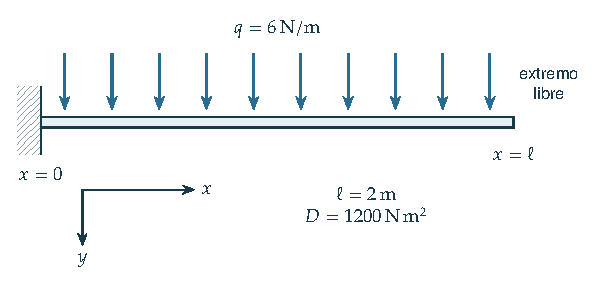
\includegraphics[width=11.34cm]{assets/M2-E0331-setup.pdf}\par
\smallskip{\small Tira empotrada y sentido positivo del desplazamiento transversal.\par}
\end{minipage}
\end{center}

\supportlinks{M2-E0331}{0}{0}
\exercise{M2-E0155}{Core · Intermedio}
Resuelva $y''+y=\tan x$ en cada intervalo de definición.

\supportlinks{M2-E0155}{0}{0}
\exercise{M2-E0093}{Core · Avanzado}
Sea \(a\in\mathbb R\). Considera la familia
\[xy''-(ax+1)y'+ay=0.\]
Resuelve en intervalos donde la ecuación sea regular y señala cómo se interpretan los casos excepcionales.

\begin{enumerate}[label=(\alph*),ref=\alph*,leftmargin=*]
\item Resuelve la ecuación sabiendo que admite una solución exponencial.
\item Determina \(a\) para que una solución no nula de la familia, usada como función \(\mu(x)\), sea factor integrante de
\[(xy^2+x^2y^2+3)\,dx+x^2y\,dy=0.\]
Halla ese factor.
\end{enumerate}

\supportlinks{M2-E0093}{0}{0}
\exercise{M2-E0157}{Core · Intermedio}
Resuelva $xy''+(5x-1)y'-5y=x^2e^{-5x}$, sabiendo que la homogénea tiene una solución $e^{ax}$ con $a$ entero. Considere intervalos regulares.

\supportlinks{M2-E0157}{0}{0}
\exercise{M2-E0153}{Core · Intermedio}
Resuelva $y^{(3)}+y'=1/\sin x$ en sus intervalos de definición.

\supportlinks{M2-E0153}{0}{0}
\exercise{M2-E0076}{Core · Avanzado}
Considera la ecuación de Hermite
\[y''-2xy'+4y=0,\qquad x\in\mathbb R.\]
Conserva el dominio de cada integral que utilices; una singularidad de una fórmula auxiliar no es necesariamente una singularidad de la solución.

\begin{enumerate}[label=(\alph*),ref=\alph*,leftmargin=*]
\item Comprueba que \(y_1=1-2x^2\) es solución.
\item Usa reducción de orden para obtener otra solución linealmente independiente. Puedes dejar una integral definida.
\item Escribe la solución general.
\end{enumerate}

\supportlinks{M2-E0076}{0}{1}
\Needspace{12\baselineskip}
\section{Síntesis, parámetros y límites}
\exercise{M2-E0161}{Core · Intermedio}
Resuelva en $\mathbb R$ las ecuaciones siguientes. Identifique el orden y la base homogénea de cada ecuación antes de calcular una particular.

\begin{enumerate}[label=(\alph*),ref=\alph*,leftmargin=*]
\item $y'-y=\sin x+\cos(2x)$.
\item $y^{(3)}+3y''-4y=\sin x$.
\item $y''-2y'+y=x^2-1$.
\item $y^{(3)}-y''+3y'+5y=4x+\sin(2x)$.
\end{enumerate}

\supportlinks{M2-E0161}{0}{0}
\exercise{M2-E0094}{Core · Avanzado}
Denota \(D=d/dx\). Discute la solución general de \(P(D)y=0\), en \(\mathbb R\), según los valores reales del parámetro a.

\begin{enumerate}[label=(\alph*),ref=\alph*,leftmargin=*]
\item \[P(D)=D^3-2(a-1)D^2+(a-1)^2D-a.\]
\item \[P(D)=D^3-\frac1aD^2-a^2D+a,\qquad a\ne0.\]
\end{enumerate}

\supportlinks{M2-E0094}{0}{0}
\exercise{M2-E0333}{Core · Intermedio}
Se considera el problema
\[
y''-y'=f(t),\qquad y(0)=0,\qquad t\ge0,
\]
en variables adimensionales. La pendiente inicial puede elegirse. Se estudian dos entradas por separado: \(f(t)=\cos t\) y \(f(t)=1\).

Elija y justifique una vía de resolución antes de efectuar los cálculos. Para cada entrada, determine si existe una pendiente inicial que mantenga \(y\) acotada durante todo \(t\ge0\). Si existe, obtenga esa pendiente y la solución correspondiente; si no, explique por qué ningún valor de la pendiente puede conseguirlo. Su argumento debe distinguir los términos que se pueden modificar mediante las condiciones iniciales de los impuestos por la entrada. Aquí «acotada» significa que existe una constante finita \(B\) tal que \(|y(t)|\le B\) para todo \(t\ge0\).

\supportlinks{M2-E0333}{0}{0}
\exercise{M2-E0095}{Core · Avanzado}
Sea \(P(D)=D^3-(2a+1)D^2+(2a+4)D-4\), con a real.

\begin{enumerate}[label=(\alph*),ref=\alph*,leftmargin=*]
\item Discute según a la solución general de \(P(D)y=0\).
\item Toma \(a=2\) y resuelve \(P(D)y=2xe^x+e^{-x}\).
\end{enumerate}

\supportlinks{M2-E0095}{0}{0}
\exercise{M2-E0334}{Core · Avanzado}
Para cada \(\varepsilon>0\), sea \(y_\varepsilon\) la solución de
\[
\varepsilon y_\varepsilon''+y_\varepsilon'=0,
\qquad y_\varepsilon(0)=a,\qquad y_\varepsilon'(0)=b,
\qquad t\ge0.
\]
Todas las variables son adimensionales; \(a\) y \(b\) son constantes reales que no dependen de \(\varepsilon\).

Obtenga \(y_\varepsilon\) y compárela con la solución de la ecuación que resulta al poner \(\varepsilon=0\), conservando el dato \(y(0)=a\). ¿Qué sucede con el otro dato inicial? Dé una cota de \(|y_\varepsilon(t)-a|\) válida simultáneamente para todo \(t\ge0\). Compare también las derivadas en \(t=0\), en un tiempo \(t>0\) fijo y en \(t=\varepsilon\). Decida si esas derivadas pueden aproximarse a la derivada de la solución reducida con un error que tienda a cero para todos los tiempos \(t\ge0\) a la vez, e indique si hay un caso excepcional. Base la respuesta en las fórmulas explícitas.

\supportlinks{M2-E0334}{1}{0}
\chapter{Oscilaciones, amortiguamiento y respuesta forzada}
\label{chapter:5}
%
\subsection*{Desplazamiento, equilibrio y energía}
\label{CH05-B01}
Fijado el sentido positivo, $m x''$ es la suma de fuerzas. Medido desde
el equilibrio estático, el oscilador lineal habitual cumple
\[
 m x''+c x'+kx=F(t),\qquad m>0,\quad k>0,\quad c\ge0.
\]
Aquí $k$ se mide en fuerza/longitud y $c$ en fuerza/velocidad. Si el
equilibrio ya incorpora el peso, no se añade éste de nuevo. Un evento
inicial exige precisar los datos inmediatamente después de él.

La frecuencia natural angular es $\omega_0=\sqrt{k/m}$, en radianes por
unidad de tiempo; la frecuencia ordinaria es $f_0=\omega_0/(2\pi)$, en
hercios si el tiempo se mide en segundos. La energía
$E=mx'^2/2+kx^2/2$ satisface $E'=F x'-c x'^2$.
Esta identidad comprueba signos y disipación. Recuérdense la segunda ley
de Newton y la derivación de productos. Consulta: solución de
\exref{M2-E0017}.

%
\subsection*{Regímenes, amplitud y envolvente}
\label{CH05-B02}
Las raíces de $mr^2+cr+k=0$ clasifican la respuesta libre. Con $c>0$,
$c^2<4mk$ da oscilación amortiguada; $c^2=4mk$, amortiguamiento crítico;
$c^2>4mk$, sobreamortiguamiento. En el primer caso,
\[
 x(t)=R e^{-ct/(2m)}\cos(\omega_d t-\phi),\qquad
 \omega_d=\sqrt{k/m-c^2/(4m^2)}.
\]
Las curvas $\pm R e^{-ct/(2m)}$ acotan la respuesta; sus valores no son
automáticamente máximos de la trayectoria, que se localizan con $x'=0$.
Tampoco una envolvente de una familia es necesariamente una trayectoria
de esa familia.

En un RLC serie ideal, la carga $q$ y la corriente $i=q'$ cumplen
$Lq''+Rq'+q/C=V(t)$; las relaciones de inductor, resistencia y
condensador fijan los signos según el circuito. Recuérdense raíces
complejas y trigonometría. Consulta: solución de \exref{M2-E0374}.

%
\subsection*{Forzamiento periódico y resonancia}
\label{CH05-B03}
Para $F(t)=F_0\cos\omega t$, $F_0>0$, una respuesta periódica puede
escribirse $A\cos(\omega t-\delta)$, donde
\[
 A=\frac{F_0}{\sqrt{(k-m\omega^2)^2+(c\omega)^2}},\qquad
 \cos\delta=\frac{k-m\omega^2}{D},\quad
 \sin\delta=\frac{c\omega}{D},
\]
con $D$ igual al denominador y $D\ne0$. Ambas razones fijan el cuadrante
del desfase. Con $c>0$, el transitorio decae. Con $c=0$ y
$\omega=\omega_0$, se necesita una particular resonante, proporcional
a $t\sin(\omega_0t)$.

El PVI conserva sus datos: al variar la frecuencia, el límite resonante
se toma sobre la respuesta completa, incluida la homogénea. En un apoyo
móvil $b(t)$, la elongación y la velocidad relativa son $x-b$ y $x'-b'$;
el balance determina dónde aparecen. Consulta: solución de
\exref{M2-E0117}.

%
\subsection*{Identificación y garantías}
\label{CH05-B04}
Una inversión algebraica puede producir varias ramas. Manténganse todas
las que respetan unidades, signos y dominio físico hasta aplicar los datos
que permiten distinguirlas. Ni un dato aislado ni un régimen final
identifican necesariamente todos los parámetros o la ley resistente.

Un intervalo garantizado describe valores posibles; no asigna
probabilidades. Para afirmar una propiedad para todos los parámetros
admisibles hace falta una cota válida en todo el conjunto. Un solo caso
admisible que la incumpla refuta esa garantía. Al buscar máximos, indíquese
si se optimiza sobre el tiempo de una trayectoria, sobre parámetros a
tiempo fijo o sobre ambos: las preguntas son diferentes. Recuérdense
desigualdades y restricciones físicas. Consultas: soluciones de
\exref{M2-E0038} y \exref{M2-E0374}.

\Needspace{12\baselineskip}
\section{Modelos, datos y escalas}
\exercise{M2-E0337}{Core · Básico}
Una masa puntual \(m>0\) está sujeta a una varilla sin masa de longitud \(\ell>0\), que gira sin rozamiento. El ángulo \(\theta\), en radianes, se mide desde la vertical inferior. El momento de inercia es \(m\ell^2\), y el único par es \(-mg\ell\sin\theta\), con \(g>0\). La ley de movimiento iguala el momento de inercia por la aceleración angular al par neto.

Construya la EDO y su aproximación al sustituir \(\sin\theta\) por \(\theta\). Se acepta esa sustitución cuando el error de par relativo al módulo del par lineal no supera el \(1\%\):
\[
E(\theta)=\frac{|\theta-\sin\theta|}{|\theta|}\le0.01
\quad(\theta\ne0),\qquad E(0)=0.
\]
Use la desigualdad \(|\theta-\sin\theta|\le|\theta|^3/6\) para dar un intervalo angular garantizado. Calcule también \(E\) en \(0.20\) y \(0.30\) rad y decida si cada ángulo cumple el criterio. Explique a qué error se refiere la garantía y si permite, por sí sola, afirmar el mismo porcentaje para una trayectoria o un periodo.

\Needspace{7.8cm}
\begin{center}
\begin{minipage}{\linewidth}
\centering
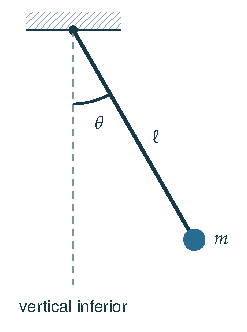
\includegraphics[width=4.69cm]{assets/M2-E0337-setup.pdf}\par
\smallskip{\small Referencia angular desde la vertical inferior.\par}
\end{minipage}
\end{center}

\supportlinks{M2-E0337}{0}{0}
\exercise{M2-E0017}{Core · Intermedio}
Un conjunto horizontal masa--resorte, con \(m=2\,\mathrm{kg}\) y \(k=8\,\mathrm{N/m}\), viaja en un camión a \(1\,\mathrm{m/s}\).
El camión se detiene bruscamente y el extremo sujeto del resorte queda fijo. La masa se libera en ese instante, situada \(0.5\,\mathrm m\) por delante del equilibrio y con velocidad hacia delante \(1\,\mathrm{m/s}\) respecto al extremo fijo.
En el modelo ideal sin rozamiento, hallar la frecuencia y la amplitud de la oscilación posterior.

\Needspace{6.53cm}
\begin{center}
\begin{minipage}{\linewidth}
\centering
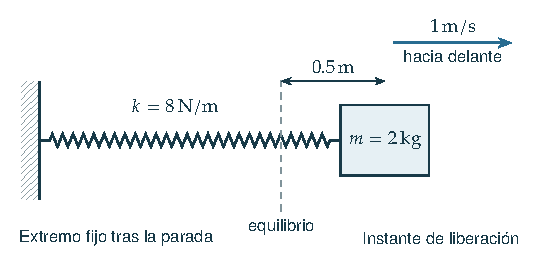
\includegraphics[width=10.22cm]{assets/M2-E0017-setup.pdf}\par
\smallskip{\small Configuración en el instante de liberación, con el extremo del muelle ya fijo.\par}
\end{minipage}
\end{center}

\supportlinks{M2-E0017}{1}{0}
\exercise{M2-E0036}{Core · Básico}
Un sistema masa--resorte--amortiguador lineal sin fuerza externa tiene \(m=2\,\mathrm{kg}\), \(k=3\,\mathrm{N/m}\) y \(c=1\,\mathrm{N\,s/m}\).

\begin{enumerate}[label=(\alph*),ref=\alph*,leftmargin=*]
\item Formular la ecuación del movimiento y encontrar su solución general.
\item Clasificar el régimen de amortiguamiento.
\item Hallar el coeficiente \(c\ge0\) que produciría amortiguamiento crítico manteniendo masa y resorte.
\end{enumerate}

\supportlinks{M2-E0036}{0}{1}
\exercise{M2-E0287}{Core · Básico}
Una masa de $2\,\mathrm{kg}$ unida a un resorte ideal parte del equilibrio con velocidad $2\,\mathrm{m/s}$. No hay amortiguamiento. Determine qué valores de la constante elástica $k>0$ impiden que se aleje más de $3\,\mathrm m$ del equilibrio.

Se usan segundos y metros. El resorte es lineal, el soporte está fijo y el desplazamiento se mide desde el equilibrio; se omiten disipación y fuerzas externas después del impulso inicial.

\supportlinks{M2-E0287}{0}{0}
\exercise{M2-E0338}{Core · Básico}
Un amortiguador viscoso ejerce la fuerza \(F_d=-c x'\), con \(c>0\). Mediante excitaciones externas, que pueden ser distintas, se mantienen estas dos respuestas periódicas de un mismo sistema masa--resorte:
\[
x_1(t)=A\cos(\omega t),\qquad x_2(t)=A\cos(2\omega t),
\qquad A,\omega>0.
\]
No hay transitorio. La energía mecánica se repite al completar cada periodo y el trabajo de una fuerza es \(\int F x'\,dt\).

Compare la energía disipada por el amortiguador en los dos ensayos, primero durante el mismo intervalo \([0,2\pi/\omega]\) y después durante un periodo propio de cada respuesta. Explique por qué los dos cocientes no coinciden e indique el signo del trabajo del amortiguador y el trabajo neto que debe aportar la excitación externa en cada intervalo considerado.

\supportlinks{M2-E0338}{0}{0}
\Needspace{12\baselineskip}
\section{Trayectorias, medidas y garantías}
\exercise{M2-E0162}{Core · Intermedio · Representación}
Una masa de $100\,\mathrm{kg}$ está unida en paralelo a un muelle de $80\,\mathrm{N/m}$ y a un amortiguador de $40\,\mathrm{N\,s/m}$. Se mide $x$ en metros, positivo hacia abajo, desde el equilibrio previo cargado por la gravedad. En $t=0$ se aplica una fuerza adicional constante de $15\,\mathrm N$, partiendo del reposo y con $x(0)=0$. Use segundos. Para estudiar la gráfica, se proporciona la solución ya obtenida del PVI $100x''+40x'+80x=15$: $x(t)=\frac3{16}\left[1-e^{-t/5}\left(\cos\frac{\sqrt{19}t}{5}+\frac1{\sqrt{19}}\sin\frac{\sqrt{19}t}{5}\right)\right]$, para $t\ge0$.

\begin{enumerate}[label=(\alph*),ref=\alph*,leftmargin=*]
\item Dibuje la gráfica del desplazamiento en función del tiempo.
\item Justifique la forma de la gráfica.
\end{enumerate}

\supportlinks{M2-E0162}{0}{0}
\exercise{M2-E0339}{Core · Intermedio}
El desplazamiento de un soporte idealizado satisface el PVI de oscilación libre
\[
x''+2x'+5x=0,\qquad x(0)=-0.40,\qquad x'(0)=2.00,
\]
con \(t\) en segundos, \(x\) en centímetros y coeficientes expresados en las unidades correspondientes. Los datos son sintéticos. La holgura permitida es asimétrica:
\[
-0.45\le x(t)\le0.37\qquad\text{para todo }t\ge0.
\]
Decida si la trayectoria cumple esta condición. Para justificarlo, localice el primer máximo positivo y controle el valor inicial y los demás extremos que puedan limitar la holgura. Distinga el extremo efectivo de una cota obtenida con la envolvente de la oscilación.

\supportlinks{M2-E0339}{0}{0}
\exercise{M2-E0037}{Core · Intermedio}
Un circuito RLC serie ideal tiene resistencia \(100\,\mathrm{m}\symup{\Omega}\), inductancia \(50\,\mathrm{mH}\) y capacidad \(5\,\mathrm F\). Se mantiene una tensión constante \(E_0\).

\begin{enumerate}[label=(\alph*),ref=\alph*,leftmargin=*]
\item Obtener una EDO para la corriente \(I\).
\item Encontrar la solución general de esa EDO.
\item Imponer \(I(0)=10\,\mathrm A\) e \(I^{\prime}(0)=0\,\mathrm{A/s}\).
\end{enumerate}

\supportlinks{M2-E0037}{0}{0}
\exercise{M2-E0374}{Core · Intermedio · Oral · Croquis a mano}
Tras posicionar una herramienta en una bancada, su pequeño desplazamiento libre se modela por
\[
x''+4x=0,
\]
con \(t\) en segundos y \(x\) en milímetros; el coeficiente cuatro tiene unidades \(\mathrm{s}^{-2}\). Los errores de arranque sólo garantizan
\[
-1\le x(0)\le1\ \mathrm{mm},\qquad
-2\le x'(0)\le2\ \mathrm{mm/s}.
\]
Cualquier pareja en ese rectángulo es admisible; no se asignan probabilidades.

Determine cotas superior e inferior ajustadas para \(x(t)\) en cada instante y dibújelas a mano en \(0\le t\le\pi/2\) s. Explique oralmente si una sola trayectoria alcanza toda la envolvente superior. Decida si esos datos garantizan la holgura \(|x(t)|\le1.30\,\mathrm{mm}\) durante ese intervalo, distinguiendo una garantía para todos los arranques de lo que puede ocurrir con uno particular.

\supportlinks{M2-E0374}{1}{0}
\Needspace{12\baselineskip}
\section{Entradas y respuesta sostenida}
\exercise{M2-E0117}{Core · Intermedio}
Una masa \(m>0\) cuelga de un resorte \(k>0\), fijo arriba. Se desprecia el amortiguamiento y se mide x hacia abajo desde el equilibrio bajo el peso. Una fuerza \(F(t)=F_0\sin(\omega t)\), con \(F_0>0\), \(\omega>0\), actúa desde \(t=0\). Inicialmente \(x(0)\)=\(x'(0)\)=0. Sea \(\omega_0=\sqrt{k/m}\).

\begin{enumerate}[label=(\alph*),ref=\alph*,leftmargin=*]
\item Formula la ecuación del movimiento.
\item Halla x(t) para \(\omega\ne\omega_0\).
\item Estudia el caso \(\omega=\omega_0\).
\end{enumerate}

\supportlinks{M2-E0117}{1}{0}
\exercise{M2-E0306}{Core · Intermedio · Representación}
Para \(\omega>0\) y una amplitud de aceleración \(F_0>0\), la respuesta de
\[x''+\omega^2x=F_0\sin(\omega t),\qquad x(0)=x'(0)=0,\]
es
\[x(t)=\frac{F_0}{2\omega^2}\big[\sin(\omega t)-\omega t\cos(\omega t)\big],\qquad t\ge0.\]
Represente gráficamente esta respuesta. Puede usar las variables sin dimensiones \(\tau=\omega t\) y \(z=2\omega^2x/F_0\).

\supportlinks{M2-E0306}{0}{0}
\exercise{M2-E0039}{Core · Intermedio}
Para \(m>0\), \(k>0\), \(c>0\), \(\omega\ge0\) y \(F_0\in\mathbb R\), deducir una solución particular de
\[mx''+cx'+kx=F_0\sin(\omega t).\]

\supportlinks{M2-E0039}{0}{0}
\exercise{M2-E0097}{Core · Intermedio}
Considera un circuito RLC en serie con generador E(t). La carga del condensador es q y la intensidad orientada de la rama es \(I=q'\). Los componentes son ideales.

\begin{enumerate}[label=(\alph*),ref=\alph*,leftmargin=*]
\item Formula la ecuación diferencial del circuito.
\item Toma \(R=0\), \(L=0.1\,\mathrm H\), \(C=0.1\,\mathrm F\), \(E(t)=120\sin(100\pi t)\,\mathrm V\). El circuito se cierra en \(t=0\); antes no circula corriente y el condensador está descargado. Halla I(t).
\end{enumerate}

\Needspace{7.34cm}
\begin{center}
\begin{minipage}{\linewidth}
\centering
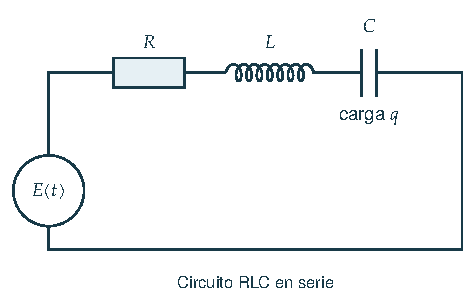
\includegraphics[width=9.02cm]{assets/M2-E0097-setup.pdf}\par
\smallskip{\small Topología del circuito RLC del apartado general.\par}
\end{minipage}
\end{center}

\supportlinks{M2-E0097}{0}{0}
\exercise{M2-E0361}{Core · Intermedio}
Una bancada horizontal idealizada tiene una masa móvil de \(10\,\mathrm{kg}\), un resorte que ejerce la fuerza \(-40x\,\mathrm N\) cuando el desplazamiento \(x\) se expresa en metros, y un amortiguador viscoso que ejerce \(-10x'\,\mathrm N\) cuando la velocidad se expresa en \(\mathrm{m/s}\). El origen es la posición de equilibrio. Un actuador aplica \(F(t)=1\cos(\omega t)\,\mathrm N\), con \(t\) en segundos. Se puede elegir únicamente \(\omega=1,2\) o \(3\,\mathrm{rad/s}\); la amplitud de la fuerza es la misma en los tres casos. Los parámetros y los criterios son sintéticos.

El ensayo se desarrolla en régimen periódico desde \(t=0\). Requiere una amplitud de desplazamiento entre \(2.5\) y \(5.5\,\mathrm{cm}\) y una potencia mecánica media entregada por el actuador no superior a \(0.020\,\mathrm W\). Esta potencia es el promedio de \(F(t)x'(t)\) durante un período completo.

Construya el modelo, elija entre las frecuencias permitidas aplicando ambos criterios y determine la posición y la velocidad iniciales que producen el régimen periódico elegido desde el comienzo. Justifique la comparación con las amplitudes y potencias de las tres opciones. Puede usar calculadora.

\supportlinks{M2-E0361}{0}{0}
\exercise{M2-E0096}{Core · Avanzado · Representación}
Una masa de \(m=100\,\mathrm{kg}\) cuelga de un resorte de rigidez \(k=80\,\mathrm{N/m}\) y un amortiguador viscoso \(c=40\,\mathrm{N\,s/m}\), en paralelo y fijados a un soporte inmóvil. Se mide x hacia abajo desde el equilibrio previo bajo la gravedad. Desde \(t=0\) actúa \(F(t)=F_0\sin(2\pi ft)\), con \(F_0>0\) en newtons, \(f=2\,\mathrm{Hz}\), y \(x(0)=x'(0)=0\). Se supone respuesta lineal y parámetros constantes.

\begin{enumerate}[label=(\alph*),ref=\alph*,leftmargin=*]
\item Formula la ecuación diferencial.
\item Obtén x(t).
\item Dibuja la respuesta.
\item ¿Qué sucedería si una frecuencia real f satisficiera
\[2\pi f=\frac{\sqrt{c^2-4km}}{2m}\ ?\]
\end{enumerate}

\supportlinks{M2-E0096}{0}{0}
\exercise{M2-E0118}{Core · Avanzado}
Una masa \(M=2\) está unida mediante un resorte \(k=2\) y un amortiguador viscoso \(c=5\), en paralelo, a una base móvil. Las cantidades se expresan en un sistema coherente de unidades. Tanto la posición de la masa x(t) como la de la base e(t) se miden hacia arriba desde el equilibrio inicial. La base sigue \(e(t)=10\sin(2\pi t)\), t>0; inicialmente la masa está en equilibrio y reposo. Halla x(t).

\Needspace{8.55cm}
\begin{center}
\begin{minipage}{\linewidth}
\centering
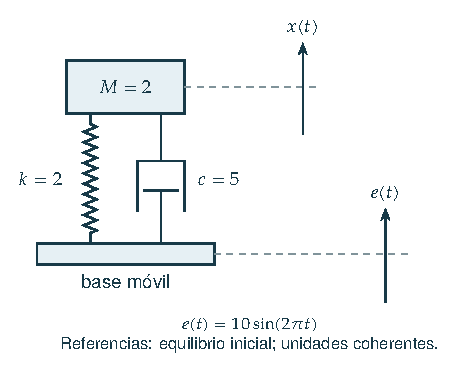
\includegraphics[width=8.7cm]{assets/M2-E0118-setup.pdf}\par
\smallskip{\small Masa y base móvil unidas mediante muelle y amortiguador en paralelo.\par}
\end{minipage}
\end{center}

\supportlinks{M2-E0118}{0}{0}
\Needspace{12\baselineskip}
\section{Decisiones y contrastes de modelos}
\exercise{M2-E0035}{Core · Intermedio}
Un vagón de \(5000\,\mathrm{kg}\) golpea a \(1\,\mathrm{m/s}\) un tope que se modela como resorte lineal y lo comprime como máximo \(0.1\,\mathrm m\). Se desprecia el amortiguamiento y cualquier otra pérdida durante la compresión; el resorte parte sin comprimir.

\begin{enumerate}[label=(\alph*),ref=\alph*,leftmargin=*]
\item Hallar la constante elástica \(k\).
\item Calcular la compresión máxima si la masa es \(10000\,\mathrm{kg}\) y la velocidad sigue siendo \(1\,\mathrm{m/s}\).
\item El resorte se rompe si se comprime más de \(0.3\,\mathrm m\). Hallar la masa máxima admisible a \(1\,\mathrm{m/s}\).
\item Hallar la masa máxima admisible si la velocidad aumenta a \(2\,\mathrm{m/s}\).
\end{enumerate}

\supportlinks{M2-E0035}{0}{0}
\exercise{M2-E0336}{Core · Intermedio}
Dos diseños idealizados tienen estas respuestas normalizadas, con \(t\ge0\) adimensional y valor de equilibrio igual a uno:
\[
y_A(t)=1-e^{-2t}(\cos t+2\sin t),\qquad
 y_B(t)=1-(1+t)e^{-t}.
\]
Para admitir un diseño se exige que el sobrepaso no exceda \(0.10\), es decir, \(y(t)\le1.10\) para todo \(t\ge0\), y que esté asentado en la banda de error \(0.05\) a partir de \(t=2\):
\[
|y(t)-1|\le0.05\qquad\text{para todo }t\ge2.
\]
Decida qué diseños cumplen ambas condiciones. Justifique una garantía válida para todo el tiempo requerido, no sólo para una lista de instantes. Puede utilizar una envolvente para obtener una cota suficiente de asentamiento; distinga esa garantía del instante exacto en que la respuesta entra por última vez en la banda, que no se pide calcular.

\supportlinks{M2-E0336}{0}{0}
\exercise{M2-E0382}{Core · Intermedio}
Una corredera de un banco de ensayo idealizado se mueve horizontalmente y está unida a un resorte de rigidez \(k=4\,\mathrm{N/m}\). Su masa es \(m=1\,\mathrm{kg}\). El desplazamiento \(x\), en metros, se mide hacia la derecha desde la posición en la que el resorte no está deformado. El resorte ejerce la fuerza \(-kx\).

Se adopta esta ley de rozamiento: mientras la corredera desliza, la fuerza de rozamiento tiene módulo \(1\,\mathrm N\) y sentido contrario a la velocidad; en reposo puede tomar cualquier valor de módulo no superior a \(1\,\mathrm N\). Si esa fuerza puede equilibrar la del resorte, la corredera permanece en reposo; si no puede, empieza a deslizar en el sentido de la fuerza elástica. No actúan otras fuerzas horizontales.

En \(t=0\) se retira, sin impulso, la sujeción que mantenía la corredera en \(x=0.60\,\mathrm m\), en reposo. Los datos y las leyes son sintéticos. Formule el modelo de cada fase que llegue a producirse y obtenga la evolución para \(t\ge0\). Localice la primera parada posterior a la liberación y decida qué ocurre después. Compruebe que la variación de energía mecánica concuerda con el trabajo del rozamiento.

\supportlinks{M2-E0382}{0}{0}
\exercise{M2-E0038}{Core · Avanzado}
Una balanza basada en un resorte con amortiguamiento viscoso tiene constantes desconocidas \(k>0\) y \(c\ge0\), iguales en todos los ensayos. Para masas patrón de \(1\,\mathrm{kg}\) y \(2\,\mathrm{kg}\) se observan frecuencias de oscilación de \(1.1\,\mathrm{Hz}\) y \(0.8\,\mathrm{Hz}\), respectivamente. Tratar estas medidas como datos exactos del modelo lineal.

\begin{enumerate}[label=(\alph*),ref=\alph*,leftmargin=*]
\item Determinar \(k\) y \(c\ge0\).
\item Obtener una fórmula para la masa a partir de una frecuencia \(f>0\), indicando cuándo hay cero, una o dos masas posibles.
\item Se mide \(f=0.2\,\mathrm{Hz}\) para un objeto cuya masa es mayor que \(1\,\mathrm{kg}\). Determinar su masa.
\end{enumerate}

\supportlinks{M2-E0038}{1}{0}
\exercise{M2-E0288}{Core · Intermedio}
Resuelva $x''+2x'+2x=4\cos t+2\sin t$, $x(0)=0$, $x'(0)=v_0$, para $v_0\in\mathbb R$, y analice la influencia de $v_0$.

\supportlinks{M2-E0288}{0}{0}
\exercise{M2-E0335}{Core · Avanzado}
Se quiere comprobar si una oscilación libre puede describirse, durante todo un ensayo, mediante
\[
x''+2\alpha x'+\omega_0^2x=0,
\qquad 0<\alpha<\omega_0,
\]
con coeficientes constantes. El tiempo se mide en segundos y el desplazamiento en centímetros. Se han registrado tres máximos positivos consecutivos; el primero define exactamente \(t=0\). Los datos sintéticos son
\[
\begin{array}{c|cc}
\text{máximo}&t\ (\mathrm s)&x\ (\mathrm{cm})\\\hline
1&0&1.000\pm0.020\\
2&2.00\pm0.02&0.500\pm0.010\\
3&4.10\pm0.02&0.250\pm0.020
\end{array}
\]
Cada \(\pm\) indica una cota de error garantizada en la escala indicada; las cotas se pueden combinar independientemente.

Use sólo los dos primeros máximos para obtener intervalos compatibles de \(\alpha\), de la frecuencia angular amortiguada \(\omega_d\) y de \(\omega_0\), distinguiendo las dos frecuencias. Reserve el tercero para contrastar por separado su instante y su altura con las predicciones del modelo. Decida si existe un modelo de coeficientes constantes compatible con todas las cotas; una discrepancia no debe atribuirse a una causa física concreta sin información adicional. Puede utilizar calculadora.

\supportlinks{M2-E0335}{0}{0}
\exercise{M2-E0370}{Core · Intermedio}
Un rotor de inercia \(J=2\,\mathrm{kg\,m^2}\) arranca desde reposo con un par motor constante de \(1\,\mathrm{N\,m}\). En un ensayo sintético alcanza un régimen estable de \(4\,\mathrm{rad/s}\). El par resistente se opone al giro, pero no se conoce su dependencia de la velocidad. El cambio de momento angular por unidad de tiempo iguala el par neto.

Formule un modelo de arranque escogiendo y justificando una ley resistente sencilla. Ajuste lo que permita el dato y prediga cuándo se alcanza la mitad de la velocidad final. Determine si otra ley razonable compatible con el mismo ensayo puede cambiar esa predicción. Proponga una medición adicional que ayude a decidir entre ellas.

\supportlinks{M2-E0370}{0}{0}
\chapter{Laplace: entradas, condiciones y respuesta}
\label{chapter:6}
%
\subsection*{Transformada unilateral y existencia}
\label{CH06-B01}
La transformada de Laplace es
$\mathcal L\{f\}(s)=\int_0^\infty e^{-st}f(t)\,dt$.
La continuidad a trozos en cada intervalo finito y una cota
$|f(t)|\le M e^{at}$ para $t$ suficientemente grande son condiciones
suficientes de convergencia para $s>a$. Hay que comprobar por separado
el origen y la cola: el factor exponencial no corrige una singularidad
no integrable en $t=0$.
\[
\begin{array}{c|c|c}
 f(t)&\mathcal L\{f\}(s)&\text{condición suficiente}\\\hline
 t^n&n!/s^{n+1}&s>0,\ n=0,1,\ldots\\
 e^{at}&1/(s-a)&s>a\\
 \cos\omega t&s/(s^2+\omega^2)&s>0\\
 \sin\omega t&\omega/(s^2+\omega^2)&s>0
\end{array}
\]
En las dos últimas filas, $\omega>0$. Las condiciones indicadas se
refieren a $s$, no al tiempo. Recuérdense integrales impropias y
exponenciales.

%
\subsection*{Propiedades y reloj de la señal}
\label{CH06-B02}
Si $F=\mathcal L\{f\}$, la transformación es lineal y
$\mathcal L\{e^{at}f(t)\}(s)=F(s-a)$. Para $a\ge0$, el escalón
$H(t-a)$ vale cero antes de $a$ y uno después; su valor aislado en $a$
no altera la transformada. La traslación temporal se escribe
\[
 \mathcal L\{H(t-a)f(t-a)\}(s)=e^{-as}F(s).
\]
Para transformar $H(t-a)g(t)$, póngase primero
$f(\tau)=g(a+\tau)$: $\tau$ mide el tiempo transcurrido desde la
activación. Reexpresar sólo una parte de la señal cambia el problema.

Si $b>0$, $\mathcal L\{f(bt)\}(s)=F(s/b)/b$. Para una señal de periodo
$T>0$, integrable y continua a trozos en un periodo,
\[
 \mathcal L\{f\}(s)=\frac{\int_0^T e^{-st}f(t)\,dt}{1-e^{-sT}},
 \qquad s>0.
\]
Una señal que alcanza una meseta no es por ello periódica.
Consulta: solución de \exref{M2-E0378}.

%
\subsection*{Transformar los datos e invertir}
\label{CH06-B03}
Con regularidad y crecimiento suficientes para integrar por partes,
\[
 \mathcal L\{y'\}=sY-y(0),\qquad
 \mathcal L\{y''\}=s^2Y-sy(0)-y'(0).
\]
En orden $n$, se restan todos los términos
$s^{n-1-j}y^{(j)}(0)$, $j=0,\ldots,n-1$. Sustitúyanse los datos con
sus signos antes de despejar $Y$. Las fracciones parciales y completar
cuadrados permiten reconocer la tabla; los factores $e^{-as}$ requieren
una traslación temporal.

Sepárese la respuesta debida a los datos de la debida a la entrada y
compruébese después la función recuperada en la ecuación y en el PVI.
Una solución puede existir para todo $t\ge0$ y crecer exponencialmente;
su transformada sólo convergerá para ciertos valores de $s$. Esta región
de convergencia no es un intervalo temporal. Consulta: solución de
\exref{M2-E0122}.

%
\subsection*{Cambios de operación y continuidad}
\label{CH06-B04}
Una señal que cambia de ley en $a$ puede escribirse como ley anterior
más $H(t-a)$ por la diferencia de leyes, expresada con el reloj adecuado.
Para varios cambios se suman las correcciones. Si una fuerza es finita
y continua a trozos, en el oscilador con masa no nula se conservan
posición y velocidad al cambiar la fuerza; la aceleración puede saltar.
Estas condiciones también enlazan las soluciones obtenidas por tramos.

Laplace resulta útil para reunir entradas activadas; resolver por tramos
puede ser más breve si hay pocos eventos. En ambos casos deben
comprobarse los empalmes, los datos y el cierre de un ciclo cuando se
pida. Que $x'(a)=0$ no demuestra que $a$ sea la primera parada, ni que
el cuerpo permanezca detenido. Apagar la fuerza tampoco añade
amortiguamiento. Consultas: soluciones de \exref{M2-E0043} y
\exref{M2-E0314}.

\Needspace{12\baselineskip}
\section{Definición, existencia y propiedades}
\exercise{M2-E0119}{Core · Básico}
Calcula, a partir de la integral unilateral \(\mathcal Lf(s)=\int_0^\infty e^{-st}f(t)\,dt\), las siguientes transformadas. Usa s real e indica dónde converge cada integral.

\begin{enumerate}[label=(\alph*),ref=\alph*,leftmargin=*]
\item \(f(t)=\sin t\).
\item \(g(t)=e^{at}\), con a real.
\item \(h(t)=t\).
\end{enumerate}

\supportlinks{M2-E0119}{0}{0}
\exercise{M2-E0121}{Core · Básico}
Sean f y g continuas a trozos en \([0,\infty)\), de orden exponencial, y sean a,b constantes reales. Demuestra la linealidad de la transformada unilateral de Laplace, para s donde ambas integrales converjan absolutamente:
\[\mathcal L(af+bg)=a\mathcal Lf+b\mathcal Lg.\]

\supportlinks{M2-E0121}{0}{0}
\exercise{M2-E0377}{Core · Básico · Oral}
Respuesta oral breve, sin tablas. Definimos la transformada para un parámetro real \(s\) mediante la integral impropia
\[
\mathcal L\{f\}(s)=\int_0^\infty e^{-st}f(t)\,dt.
\]
Sean \(f_1(t)=t^{-1/2}\) y \(f_2(t)=t^{-1}\) para \(0<t\le1\), ambas cero para \(t>1\), y \(f_1(0)=f_2(0)=0\). Sea además \(f_3(t)=e^{t^2}\). Decida para qué valores reales de \(s\) converge cada integral y justifique sin calcularla exactamente. Distinga lo que ocurre cerca de cero de lo que ocurre en el infinito. ¿Qué muestra el primer caso sobre las hipótesis \emph{suficientes} habituales de continuidad a trozos y orden exponencial? ¿Puede arreglarse el segundo cambiando sólo el valor de \(f_2(0)\)?

\supportlinks{M2-E0377}{0}{0}
\exercise{M2-E0212}{Core · Básico}
Trabaje con la transformada unilateral $\mathcal L\{f\}(s)=\int_0^\infty e^{-st}f(t)\,dt$. Las funciones de entrada son causales. Use $H(t-a)=0$ para $t<a$ y $H(t-a)=1$ para $t\ge a$; sus valores aislados en saltos no alteran la transformada.

\begin{enumerate}[label=(\alph*),ref=\alph*,leftmargin=*]
\item Calcule $\mathcal L\{2e^{-t}+4e^t\}$.
\item Calcule $\mathcal L\{8\sin t+t^2\}$.
\item Calcule $\mathcal L\{\sinh(3t)+\cosh(3t)\}$.
\item Calcule $\mathcal L\{e^{2t}\cos t\}$.
\item Calcule $\mathcal L\{te^{2t}\}$.
\end{enumerate}

\supportlinks{M2-E0212}{0}{0}
\exercise{M2-E0286}{Core · Básico}
Sea $f$ continua a trozos en $[0,\infty)$ y de orden exponencial. Si $F(s)=\mathcal L\{f\}(s)$, enuncie y demuestre la propiedad de traslación correspondiente a multiplicar $f(t)$ por $e^{at}$, con $a\in\mathbb R$.

\supportlinks{M2-E0286}{0}{0}
\Needspace{12\baselineskip}
\section{Señales y origen del tiempo}
\exercise{M2-E0281}{Core · Básico}
Escriba mediante el escalón de Heaviside la función $f(t)=0$ si $t<\pi$ y $f(t)=\sin t$ si $t\ge\pi$.

\supportlinks{M2-E0281}{0}{0}
\exercise{M2-E0120}{Core · Básico}
Sea \(a\ge0\), y sea f una función continua a trozos en \([0,\infty)\) de orden exponencial. Denota por u el escalón unitario. Demuestra la segunda propiedad de traslación de Laplace:
\[\mathcal L\{f(t-a)u(t-a)\}(s)=e^{-as}\mathcal L\{f(t)\}(s),\]
para s en la región de convergencia absoluta.

\supportlinks{M2-E0120}{0}{0}
\exercise{M2-E0378}{Core · Básico}
Un controlador conecta una orden de rampa en \(t=2\); antes de ese instante la orden es cero. El tiempo y la orden están normalizados y son adimensionales. En el programa A, al conectarse se usa la lectura del reloj que funciona desde \(t=0\). En el programa B se usa un reloj que se pone a cero al conectarse. La orden es igual a la lectura del reloj correspondiente.

Construya las dos señales, calcule sus transformadas de Laplace e indique para qué \(s\) reales existen. Al aplicar un desplazamiento, identifique qué función del tiempo transcurrido está trasladando. Explique la diferencia entre las órdenes recibidas por el actuador justo después de conectar. ¿Impiden una transformada el salto finito o la elección del valor de la señal en el instante exacto de conexión?

\supportlinks{M2-E0378}{1}{0}
\exercise{M2-E0282}{Core · Básico}
Escriba mediante funciones de Heaviside el pulso $f(t)=t$ para $0\le t<1$, $f(t)=2-t$ para $1\le t<2$ y $f(t)=0$ en otro caso.

\supportlinks{M2-E0282}{0}{0}
\exercise{M2-E0283}{Core · Básico}
Para $a>0$, calcule la transformada unilateral de Laplace de $f(t)=t$ cuando $0\le t<a$ y $f(t)=0$ cuando $t\ge a$.

\supportlinks{M2-E0283}{0}{0}
\exercise{M2-E0122}{Core · Intermedio}
Resuelve mediante Laplace los tres PVI siguientes para t\ensuremath{\ge}0. En cada caso comprueba el resultado por sustitución directa.

\begin{enumerate}[label=(\alph*),ref=\alph*,leftmargin=*]
\item \(y''+y=t^2+2,\ y(0)=1,\ y'(0)=-1\).
\item \(y''-y'-2y=0,\ y(0)=-2,\ y'(0)=5\).
\item \(y''+2y'+2y=\sin t,\ y(0)=1,\ y'(0)=1\).
\end{enumerate}

\supportlinks{M2-E0122}{1}{0}
\exercise{M2-E0043}{Core · Intermedio}
Resolver para \(t\ge0\) el modelo normalizado
\[x''+x=f(t),\quad x(0)=x'(0)=0,\qquad
f(t)=\begin{cases}1,&1\le t<5,\\0,&\text{en otro caso}.\end{cases}\]
La entrada representa una fuerza que se activa en \(t=1\) y se apaga en \(t=5\).

\supportlinks{M2-E0043}{1}{0}
\exercise{M2-E0044}{Core · Intermedio}
Sea \(f(t)=(t-1)^2\) si \(1\le t<2\), \(f(t)=3-t\) si \(2\le t<3\), y \(f(t)=0\) en otro caso. Para \(t\ge0\):

\begin{enumerate}[label=(\alph*),ref=\alph*,leftmargin=*]
\item Escribir \(f\) mediante escalones.
\item Resolver \(x''+x=f(t)\), \(x(0)=x'(0)=0\), mediante Laplace.
\end{enumerate}

\supportlinks{M2-E0044}{0}{0}
\exercise{M2-E0126}{Core · Intermedio}
La función f es la rampa seguida de una meseta indicada en la figura, con T>0. Es cero para t<0.
\begin{center}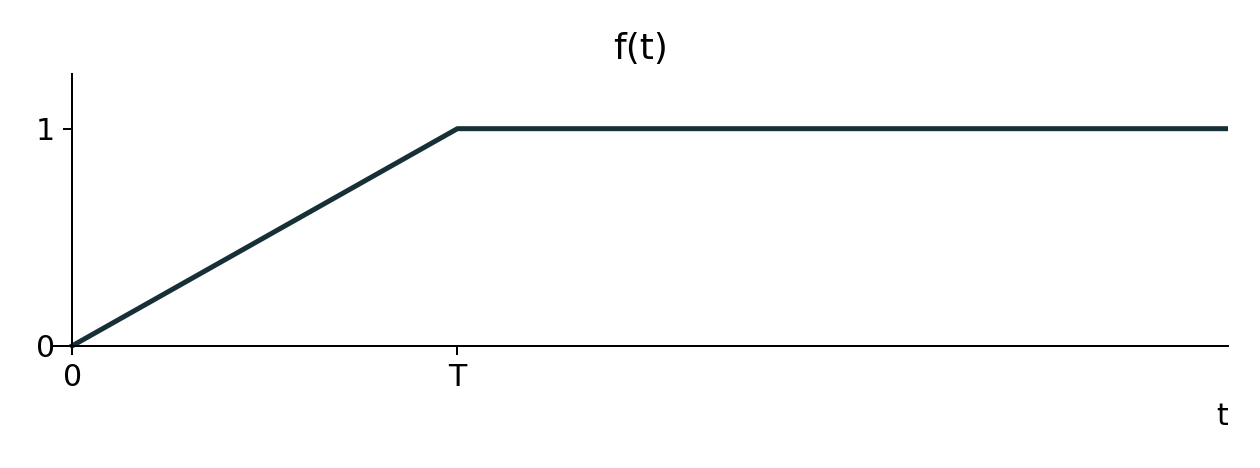
\includegraphics[width=.75\linewidth]{assets/M2-E0126-input.png}\end{center}

\begin{enumerate}[label=(\alph*),ref=\alph*,leftmargin=*]
\item Halla la transformada de f.
\item Para a real, resuelve la familia \(y'+ay=f(t)\), \(y(0)\)=0.
\end{enumerate}

\supportlinks{M2-E0126}{0}{0}
\Needspace{12\baselineskip}
\section{Condiciones y evolución}
\exercise{M2-E0042}{Core · Intermedio}
Resolver mediante Laplace \(mx''+cx'+kx=0\), \(x(0)=a\), \(x'(0)=b\), para \(t\ge0\), donde \(m,c,k>0\) y \(c^2>4km\).

\supportlinks{M2-E0042}{0}{0}
\exercise{M2-E0079}{Core · Intermedio}
Usa la transformada unilateral de Laplace para resolver los siguientes PVI en \(t\ge0\). En los cambios de entrada, interpreta la solución como continua y la ecuación en cada intervalo abierto.

\begin{enumerate}[label=(\alph*),ref=\alph*,leftmargin=*]
\item \[y'+y=f(t),\quad y(0)=0,\qquad f(t)=\begin{cases}1-t&0\le t<1,\\t-1&1\le t<2,\\1&t\ge2.\end{cases}\]
\item \[y'-y=g(t),\quad y(0)=0,\qquad g(t)=\begin{cases}t^2&0\le t<2,\\0&t\ge2.\end{cases}\]
\end{enumerate}

\supportlinks{M2-E0079}{0}{0}
\exercise{M2-E0124}{Core · Intermedio}
Usa Laplace para resolver
\[mx''+cx'+kx=0,\quad x(0)=a,\quad x'(0)=b,\]
con \(m,c,k>0\), \(c^2<4km\) y datos reales a,b.

\supportlinks{M2-E0124}{0}{0}
\exercise{M2-E0128}{Core · Intermedio · Representación}
Una masa de 100 kg cuelga de un resorte de 80 N/m y un amortiguador viscoso de 40 N·s/m, dispuestos en paralelo y fijados a un soporte inmóvil. Mide x hacia abajo desde el equilibrio previo bajo el peso. Una fuerza adicional de 15 N actúa hacia abajo durante 8 s y luego se retira. En \(t=0\), x=x\ensuremath{^{\prime}}=0. Se suponen componentes lineales y parámetros constantes.

\begin{enumerate}[label=(\alph*),ref=\alph*,leftmargin=*]
\item Formula la ecuación diferencial.
\item Obtén x(t).
\item Dibuja la gráfica.
\end{enumerate}

\supportlinks{M2-E0128}{0}{0}
\exercise{M2-E0041}{Core · Intermedio}
Una muestra contiene inicialmente \(1\,\mathrm g\) de una sustancia radiactiva cuya tasa de degradación es proporcional a la cantidad presente, con constante \(1\,\mathrm{min^{-1}}\). Desde \(t=1\,\mathrm{min}\) hasta \(t=10\,\mathrm{min}\) se añade la misma sustancia a \(0.5\,\mathrm{g/min}\); después se interrumpe la alimentación. Determinar la cantidad para \(t\ge0\).

\supportlinks{M2-E0041}{0}{0}
\exercise{M2-E0284}{Core · Intermedio}
Resuelva para $t\ge0$ el PVI $x''+x=f(t)$, $x(0)=x'(0)=0$, donde $f=0$ para $t<1$, $f=t-1$ para $1\le t<2$ y $f=1$ para $t\ge2$.

\supportlinks{M2-E0284}{0}{0}
\exercise{M2-E0213}{Core · Intermedio}
Trabaje con la transformada unilateral $\mathcal L\{f\}(s)=\int_0^\infty e^{-st}f(t)\,dt$. Las funciones de entrada son causales. Use $H(t-a)=0$ para $t<a$ y $H(t-a)=1$ para $t\ge a$; sus valores aislados en saltos no alteran la transformada. Resuelva por Laplace, para $t\ge0$,
\[y''-y=f(t),\quad y(0)=1,\quad y'(0)=-1,\qquad f(t)=\begin{cases}\sin t,&0\le t\le2\pi,\\0,&t>2\pi.\end{cases}\]

\supportlinks{M2-E0213}{0}{0}
\Needspace{12\baselineskip}
\section{Repetición, ciclos y lectura de entradas}
\exercise{M2-E0125}{Core · Intermedio}
Las gráficas muestran un pulso triangular f y una sucesión periódica g de esos pulsos. Sean \(a,h>0\) y \(b>2a\); ambas funciones son cero para t<0. Los ejes y vértices fijan la altura h, la anchura 2a y el periodo b.
\begin{center}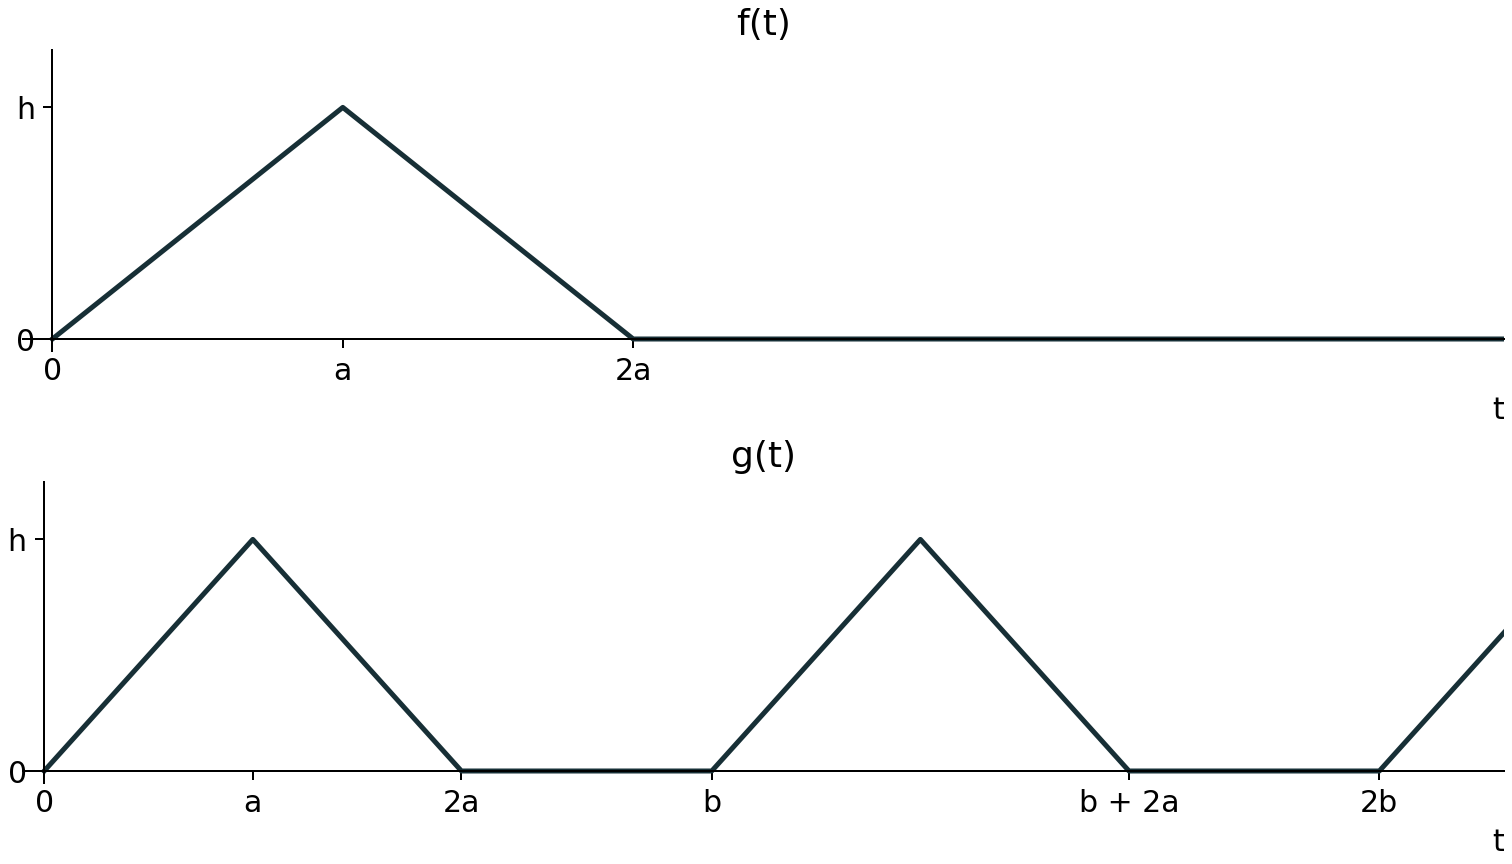
\includegraphics[width=.95\linewidth]{assets/M2-E0125-input.png}\end{center}

\begin{enumerate}[label=(\alph*),ref=\alph*,leftmargin=*]
\item Calcula la transformada de f.
\item Calcula la transformada de g.
\item Toma \(a=1\), \(h=4\) y resuelve \(y'+2y=f(t)\), \(y(0)\)=0.
\end{enumerate}

\supportlinks{M2-E0125}{0}{0}
\exercise{M2-E0340}{Core · Intermedio}
Un circuito serie idealizado permanece cerrado y contiene una resistencia \(R=1\,\Omega\) y una inductancia \(L=1\) H. Sus caídas de tensión son \(Ri\) y \(Li'\), y su suma iguala la tensión de la fuente. En cada ciclo de tres segundos, la fuente proporciona \(6\) V durante el primer segundo y \(0\) V durante los dos siguientes; la operación se repite indefinidamente. Los valores son sintéticos.

Formule la entrada periódica y la ecuación para la corriente. Elija y justifique una herramienta de resolución adecuada para obtener la operación periódica. Determine qué corriente debe existir al comienzo del primer ciclo para que la respuesta sea periódica desde ese instante, y dé la corriente durante un ciclo completo. Distinga esa inicialización de lo que ocurre al empezar con otra corriente. Obtenga además la corriente media de un ciclo integrando el balance de tensión, sin calcular por separado la integral de cada tramo de la solución.

\supportlinks{M2-E0340}{0}{0}
\exercise{M2-E0383}{Core · Intermedio}
Un pequeño equipo de ensayo idealizado tiene temperatura uniforme \(T\), capacidad térmica constante \(C=600\,\mathrm{J/K}\) y está en aire a \(20\,{}^\circ\mathrm C\). Elevar su temperatura en \(\Delta T\) requiere una energía \(C\Delta T\). La potencia que cede al aire es \(H(T-20)\), con \(H=10\,\mathrm{W/K}\); las diferencias de temperatura se expresan en kelvin o, con el mismo valor numérico, en grados Celsius.

Un calefactor aporta \(400\,\mathrm W\) cuando está encendido y cero cuando está apagado. Un termostato mide directamente la temperatura del equipo: apaga el calefactor al llegar a \(40\,{}^\circ\mathrm C\), lo enciende al bajar a \(30\,{}^\circ\mathrm C\) y mantiene la posición anterior del interruptor entre ambos umbrales. La conmutación no tiene retardo ni aporta energía de forma instantánea. No hay otras fuentes ni pérdidas de calor. Los datos son sintéticos.

En \(t=0\), el equipo está a \(30\,{}^\circ\mathrm C\) y el calefactor acaba de encenderse. Elija la información necesaria para describir su estado y formule el modelo. Obtenga la temperatura durante un ciclo completo, su duración y la fracción de tiempo en que el calefactor permanece encendido. Calcule también la temperatura media de un ciclo mediante el balance de energía, sin integrar por separado las dos expresiones de temperatura. Explique si conocer únicamente \(T=35\,{}^\circ\mathrm C\) permite determinar la derivada temporal de la temperatura.

\supportlinks{M2-E0383}{0}{0}
\exercise{M2-E0215}{Core · Intermedio}
Trabaje con la transformada unilateral $\mathcal L\{f\}(s)=\int_0^\infty e^{-st}f(t)\,dt$. Las funciones de entrada son causales. Use $H(t-a)=0$ para $t<a$ y $H(t-a)=1$ para $t\ge a$; sus valores aislados en saltos no alteran la transformada. Las gráficas continúan con el patrón indicado: $f$ alterna rampas de pendiente $1$ y mesetas, todas de duración $1$; $g$ repite su tramo de longitud $2$.
\begin{center}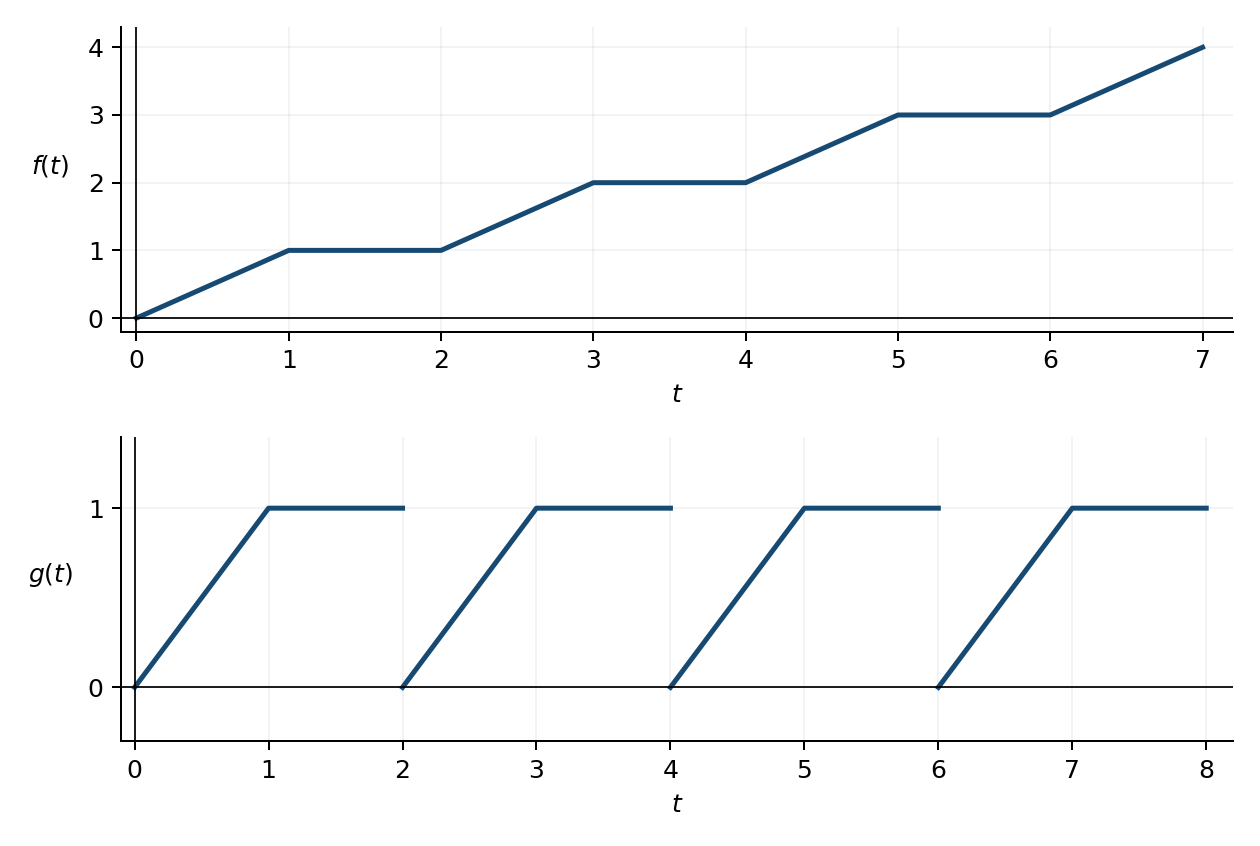
\includegraphics[width=.9\linewidth]{assets/M2-E0215-inputs.png}\end{center}

\begin{enumerate}[label=(\alph*),ref=\alph*,leftmargin=*]
\item Calcule $F(s)=\mathcal L\{f\}(s)$.
\item Resuelva por Laplace $y'+y=f(t)$, $y(0)=0$.
\item Calcule la transformada de la función periódica $g$.
\end{enumerate}

\supportlinks{M2-E0215}{0}{0}
\exercise{M2-E0214}{Core · Intermedio}
Trabaje con la transformada unilateral $\mathcal L\{f\}(s)=\int_0^\infty e^{-st}f(t)\,dt$. Las funciones de entrada son causales. Use $H(t-a)=0$ para $t<a$ y $H(t-a)=1$ para $t\ge a$; sus valores aislados en saltos no alteran la transformada. Sea $f$ el pulso triangular con vértices $(0,0),(1,1),(2,0)$ y nulo fuera de $[0,2]$. Se dispone de
\[F(s)=\frac{(1-e^{-s})^2}{s^2}.\]
Las gráficas definen $g$ y $h$ (nulas después del último intervalo mostrado).
\begin{center}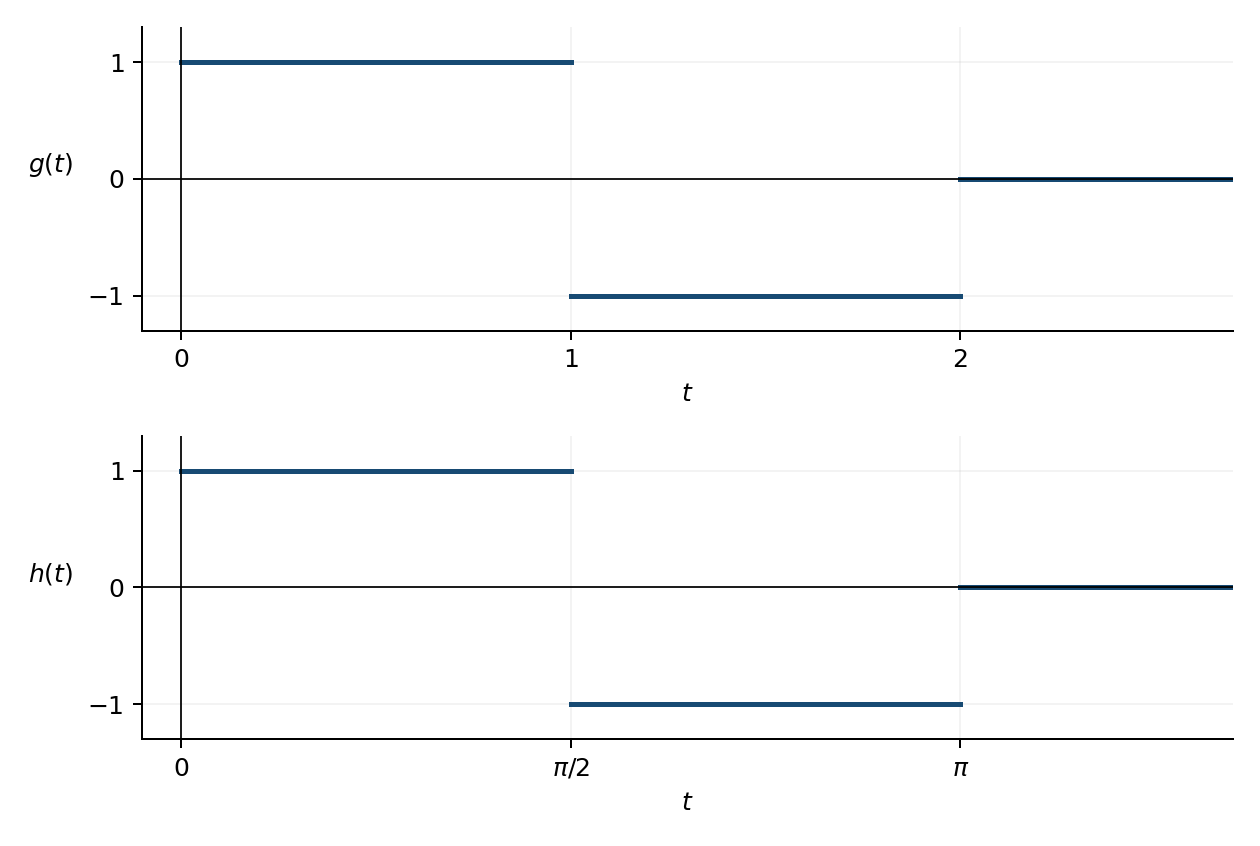
\includegraphics[width=.9\linewidth]{assets/M2-E0214-inputs.png}\end{center}

\begin{enumerate}[label=(\alph*),ref=\alph*,leftmargin=*]
\item Calcule la transformada de $g$, observando su relación con $f$.
\item Calcule la transformada de $h$, observando su relación con $g$.
\item Resuelva $y''+y=h(t)$, $y(0)=y'(0)=0$.
\end{enumerate}

\supportlinks{M2-E0214}{0}{0}
\exercise{M2-E0123}{Core · Intermedio}
Utiliza Laplace para resolver, en t\ensuremath{\ge}0,
\[y'-y=f(t),\quad y(0)=0,\qquad f(t)=\begin{cases}e^{-t}&0\le t<3,\\0&t\ge3.\end{cases}\]

\supportlinks{M2-E0123}{0}{0}
\exercise{M2-E0217}{Core · Intermedio}
Trabaje para $t\ge0$ con la transformada unilateral de Laplace y entradas causales. Use $H(t-a)=0$ para $t<a$ y $H(t-a)=1$ para $t\ge a$; los valores aislados en saltos no alteran la transformada. Use Laplace para demostrar que la solución de
\[y''+y=|\sin t|,\qquad y(0)=y'(0)=0\]
en $n\pi\le t\le(n+1)\pi$, $n=0,1,2,\ldots$, es
\[y(t)=\tfrac12(\sin t-t\cos t)+(\sin t-t\cos t)\sum_{j=1}^n(-1)^j+\pi\cos t\sum_{j=1}^n j(-1)^j.\]
Para $n=0$ ambas sumas son vacías.

\supportlinks{M2-E0217}{0}{0}
\Needspace{12\baselineskip}
\section{Reconstrucción y problemas de cierre}
\exercise{M2-E0226}{Core · Intermedio}
Trabaje para $t\ge0$ con la transformada unilateral de Laplace y entradas causales. Use $H(t-a)=0$ para $t<a$ y $H(t-a)=1$ para $t\ge a$; los valores aislados en saltos no alteran la transformada. Sean $a,b,h>0$. Las gráficas definen el pulso $f$ y la sucesión $g$, que alterna el signo de pulsos consecutivos sin intervalo entre ellos y continúa indefinidamente. Los lados oblicuos son rectos y $L=2a+b$.
\begin{center}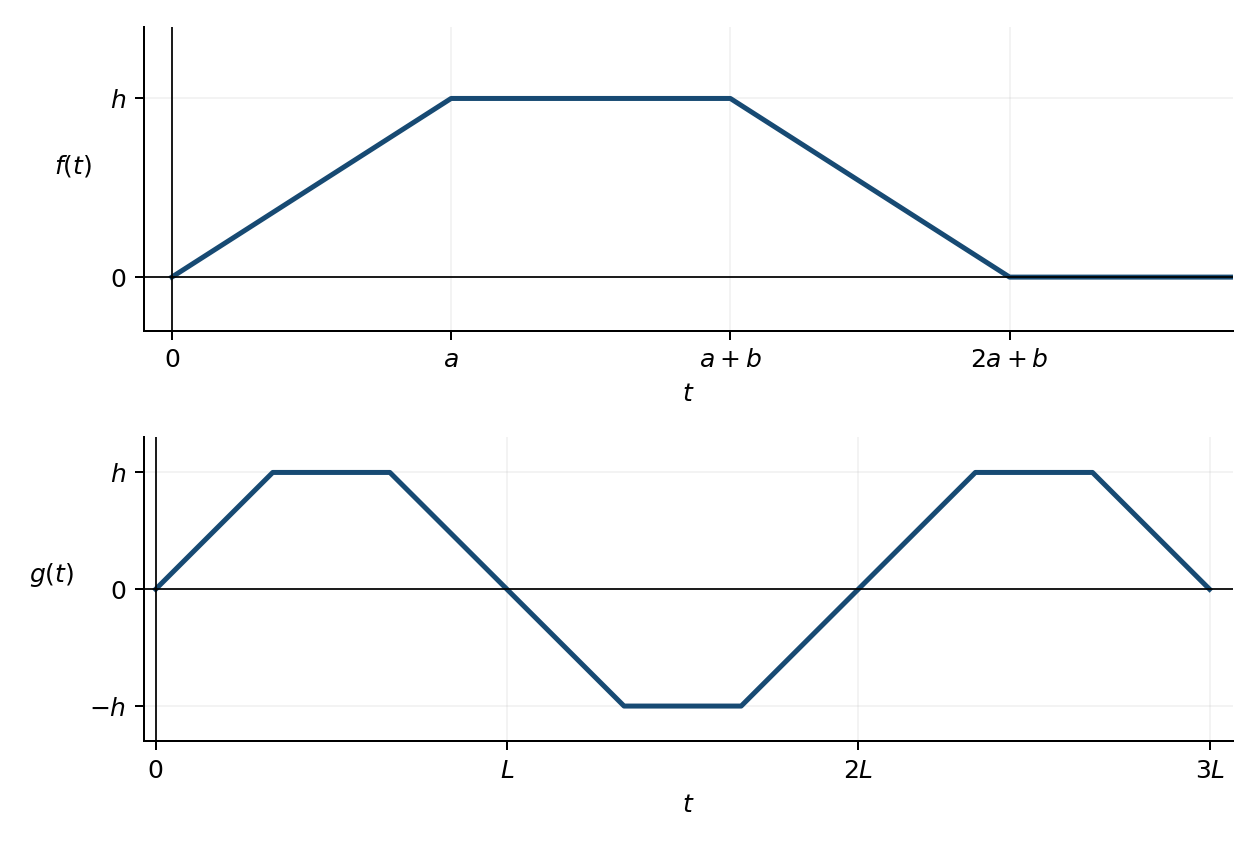
\includegraphics[width=.95\linewidth]{assets/M2-E0226-inputs.png}\end{center}

\begin{enumerate}[label=(\alph*),ref=\alph*,leftmargin=*]
\item Calcule la transformada de $f$.
\item Calcule la transformada de $g$.
\item Para $a=b=h=1$, resuelva $y'+y=g(t)$, $y(0)=0$.
\end{enumerate}

\supportlinks{M2-E0226}{0}{0}
\exercise{M2-E0341}{Core · Intermedio}
Un sistema adimensional satisface
\[
y''+3y'+2y=u(t),\qquad y(0)=y'(0)=0.
\]
Se sabe que la entrada es un único pulso de altura finita:
\[
u(t)=A\quad(0\le t<\tau),\qquad
u(t)=0\quad(t>\tau),\qquad A>0,\quad0<\tau<1.
\]
Se desconoce tanto \(A\) como \(\tau\). El registro sintético de la respuesta sólo está disponible después de \(t=1\) y se trata como exacto:
\[
y(t)=2e^{-t}-3e^{-2t}\qquad(t\ge1).
\]
Recupere la altura y la duración del pulso, y reconstruya la respuesta anterior al registro. Use explícitamente las condiciones de unión que impone una entrada finita en \(t=\tau\); indique qué derivadas pueden cambiar de valor al conmutar. El valor aislado que se asigne a la entrada en el instante del cambio no forma parte de la inferencia.

\supportlinks{M2-E0341}{0}{0}
\exercise{M2-E0227}{Core · Intermedio}
Trabaje para $t\ge0$ con la transformada unilateral de Laplace y entradas causales. Use $H(t-a)=0$ para $t<a$ y $H(t-a)=1$ para $t\ge a$; los valores aislados en saltos no alteran la transformada. Sea
\[f(t)=\begin{cases}2\sin t,&0\le t<\pi,\\0,&t\ge\pi.\end{cases}\]
La gráfica de $g$ es una versión de este semiseno con las escalas de tiempo y amplitud indicadas; fuera del arco es cero.
\begin{center}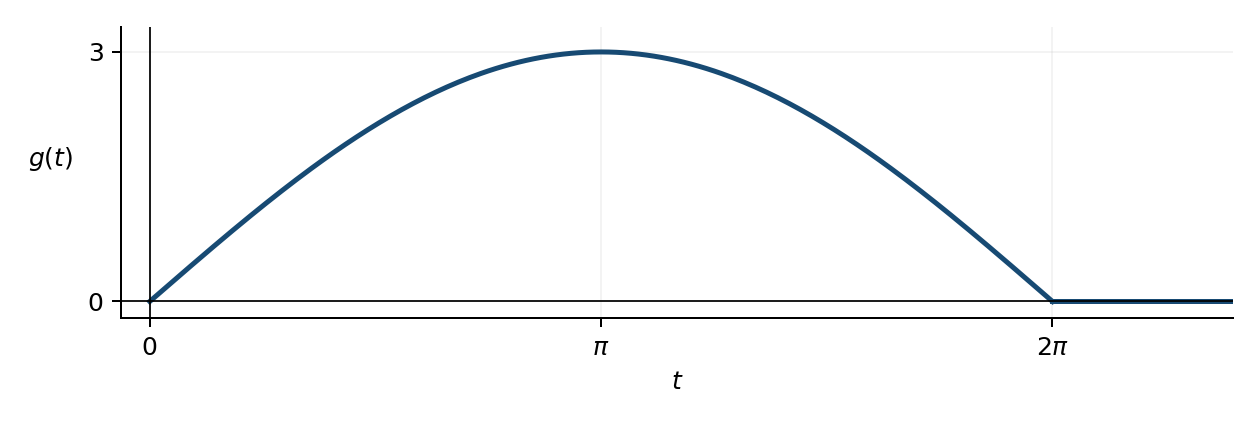
\includegraphics[width=.9\linewidth]{assets/M2-E0227-input.png}\end{center}

\begin{enumerate}[label=(\alph*),ref=\alph*,leftmargin=*]
\item Calcule la transformada de $f$.
\item Utilizando el apartado anterior, calcule la transformada de $g$.
\item Resuelva $y''-4y=f(t)$, $y(0)=0$, $y'(0)=1$.
\end{enumerate}

\supportlinks{M2-E0227}{0}{0}
\exercise{M2-E0304}{Core · Avanzado}
Resuelva, para \(t\ge0\),
\[x'''+x=(t-1)^3H(t-1),\qquad x(0)=1,\quad x'(0)=x''(0)=0,\]
donde \(H\) es el escalón de Heaviside. Su valor en cero no afecta al producto del segundo miembro.

\supportlinks{M2-E0304}{0}{0}
\exercise{M2-E0228}{Core · Intermedio}
Trabaje para $t\ge0$ con la transformada unilateral de Laplace y entradas causales. Use $H(t-a)=0$ para $t<a$ y $H(t-a)=1$ para $t\ge a$; los valores aislados en saltos no alteran la transformada. Sea
\[f(t)=\begin{cases}9-t^2,&0\le t<3,\\0,&t\ge3.\end{cases}\]
La gráfica de $g$ es una versión de esta parábola con las escalas indicadas, y es cero después del arco.
\begin{center}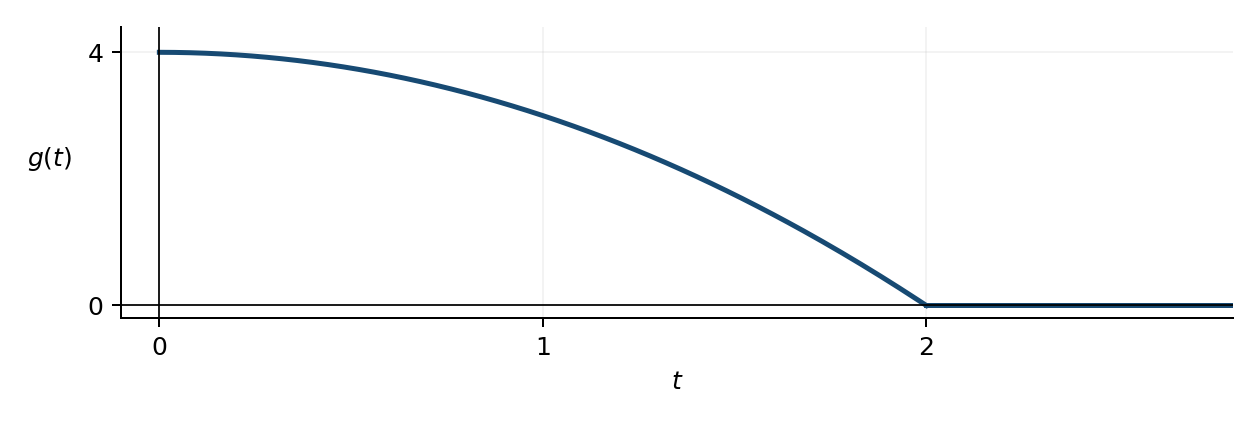
\includegraphics[width=.9\linewidth]{assets/M2-E0228-input.png}\end{center}

\begin{enumerate}[label=(\alph*),ref=\alph*,leftmargin=*]
\item Calcule la transformada de $f$.
\item Utilizando el resultado anterior, calcule la transformada de $g$.
\item Resuelva $y''+y=f(t)$, $y(0)=y'(0)=0$.
\end{enumerate}

\supportlinks{M2-E0228}{0}{0}
\exercise{M2-E0229}{Core · Intermedio}
Trabaje para $t\ge0$ con la transformada unilateral de Laplace y entradas causales. Use $H(t-a)=0$ para $t<a$ y $H(t-a)=1$ para $t\ge a$; los valores aislados en saltos no alteran la transformada. El pulso $f$ es lineal entre los vértices $(0,0),(1,1),(2,0)$ y nulo para $t\ge2$. Se dispone de $F(s)=(1-e^{-s})^2/s^2$. Resuelva por Laplace
\[y''+y=f(t),\qquad y(0)=0,\qquad y'(0)=1.\]

\supportlinks{M2-E0229}{0}{0}
\exercise{M2-E0230}{Core · Intermedio}
Trabaje para $t\ge0$ con la transformada unilateral de Laplace y entradas causales. Use $H(t-a)=0$ para $t<a$ y $H(t-a)=1$ para $t\ge a$; los valores aislados en saltos no alteran la transformada. Sea $f$ el triángulo de vértices $(0,0),(1,1),(2,0)$, nulo después de $2$, con transformada conocida $F(s)=(1-e^{-s})^2/s^2$. Las gráficas definen $g$ y $h$: $g$ es cero después del último triángulo; $h$ repite indefinidamente el patrón de longitud $6$.
\begin{center}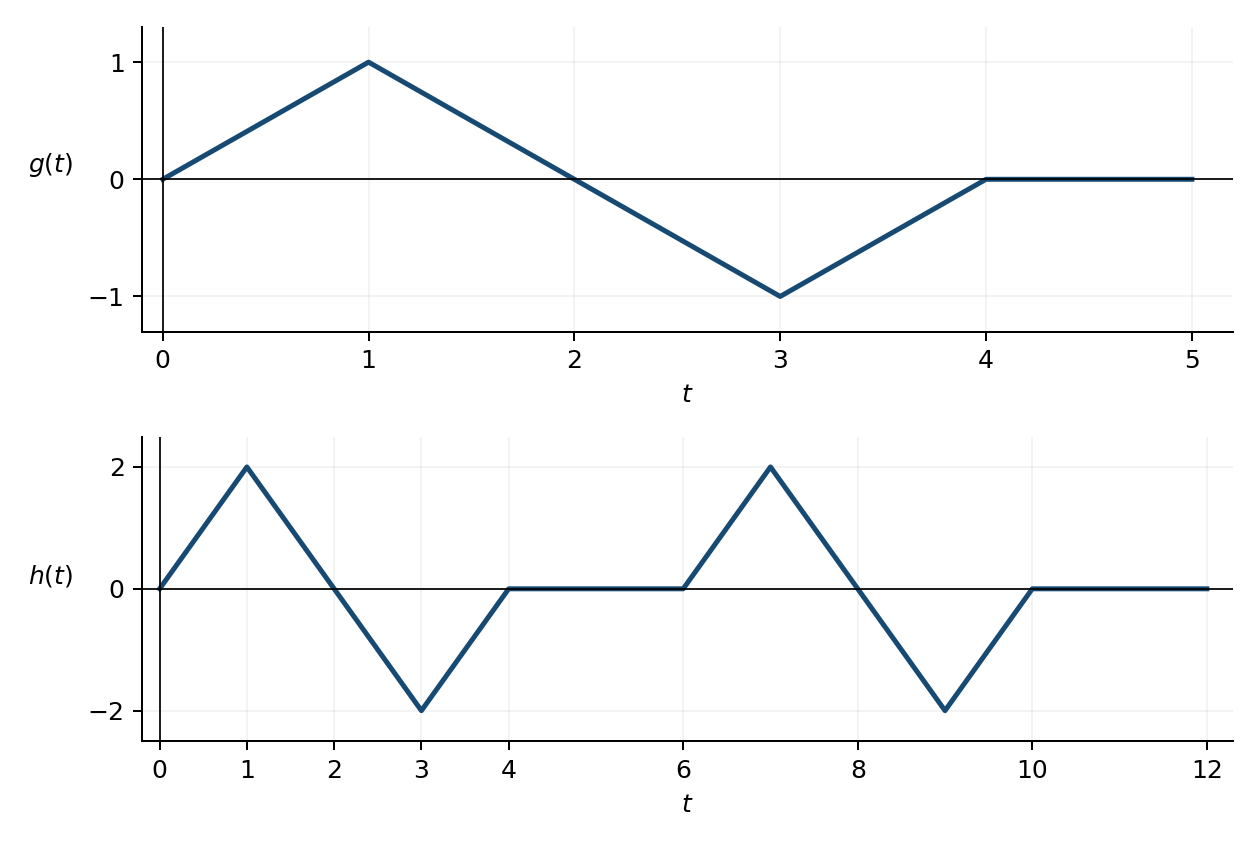
\includegraphics[width=.95\linewidth]{assets/M2-E0230-inputs.png}\end{center}

\begin{enumerate}[label=(\alph*),ref=\alph*,leftmargin=*]
\item Obtenga la transformada de $g$ utilizando $F$.
\item Calcule la transformada de $h$.
\item Resuelva $y''+y=g(t)$, $y(0)=y'(0)=0$.
\end{enumerate}

\supportlinks{M2-E0230}{0}{0}
\exercise{M2-E0127}{Core · Intermedio}
Sea \(f(t)=1\) para 0\ensuremath{\le}t\ensuremath{\le}\ensuremath{\pi} y f(t)=0 para t>\ensuremath{\pi}. Las ecuaciones con saltos de entrada se interpretan por tramos, con continuidad de la solución y las derivadas de orden inferior al principal.

\begin{enumerate}[label=(\alph*),ref=\alph*,leftmargin=*]
\item Calcula F(s).
\item Halla la solución de \(y'''-y''+y'-y=f(t)\), con \(y(0)\)=\(y'(0)\)=\(y''(0)\)=0.
\end{enumerate}

\supportlinks{M2-E0127}{0}{0}
\exercise{M2-E0314}{Core · Avanzado}
En un banco de ensayo simulado, una pieza de \(1\,\mathrm{kg}\) se mueve horizontalmente. Si \(x\) es su desplazamiento desde el equilibrio, el resorte ejerce \(-kx\), con \(k=1\,\mathrm{N/m}\), y el amortiguador ejerce \(-cx'\), con \(c=2\,\mathrm{N\,s/m}\). Inicialmente \(x(0)=x'(0)=0\). La fuerza externa es \(1\,\mathrm N\) durante el primer segundo, \(b\,\mathrm N\) durante el segundo y cero después; \(b\) puede tener cualquier signo. No hay golpes ni impulsos ideales.

El accionamiento debe conseguir que la primera parada después de arrancar ocurra en \(t=2\,\mathrm s\). Construya un modelo del movimiento que permita determinar \(b\) y elija un procedimiento de resolución, justificándolo. Calcule el nivel de fuerza necesario y el desplazamiento en ese instante. Determine también cómo evoluciona la pieza después de apagar la fuerza.

\supportlinks{M2-E0314}{1}{0}
\exercise{M2-E0216}{Core · Intermedio · Representación}
Trabaje con la transformada unilateral $\mathcal L\{f\}(s)=\int_0^\infty e^{-st}f(t)\,dt$. Las funciones de entrada son causales. Use $H(t-a)=0$ para $t<a$ y $H(t-a)=1$ para $t\ge a$; sus valores aislados en saltos no alteran la transformada. Considere
\[f(t)=\begin{cases}t,&0\le t<1,\\-2t+3,&1\le t<2,\\2t-5,&2\le t<3,\\-t+4,&3\le t<4,\\0,&t\ge4.\end{cases}\]

\begin{enumerate}[label=(\alph*),ref=\alph*,leftmargin=*]
\item Represente gráficamente $f$.
\item Calcule la transformada de $f$.
\item Resuelva $y''+y=f(t)$, $y(0)=0$, $y'(0)=1$.
\end{enumerate}

\supportlinks{M2-E0216}{0}{0}
\exercise{M2-E0129}{Core · Avanzado}
Una masa m está unida arriba a un soporte fijo mediante un resorte \(k_1\) y un amortiguador \(c_2\) en paralelo. Un segundo resorte \(k_3\) une la masa al apoyo inferior móvil P. Los desplazamientos x de la masa y f de P se miden hacia abajo desde el equilibrio inicial. Inicialmente \(x(0)\)=\(x'(0)\)=0. Los parámetros, en SI, son \(k_1=2\,\mathrm{N/m}\), \(c_2=5\,\mathrm{N\,s/m}\), \(k_3=3\,\mathrm{N/m}\), \(m=1\,\mathrm{kg}\). Se consideran resortes y amortiguador lineales.

\begin{enumerate}[label=(\alph*),ref=\alph*,leftmargin=*]
\item Halla x(t) si \(f(t)=\sin(2t)\,\mathrm{cm}\).
\item Halla x(t) si P baja a velocidad 0.01 m/s durante 10 s y luego permanece inmóvil.
\item Clasifica el amortiguamiento y calcula su razón \(\zeta\).
\end{enumerate}

\Needspace{9.030000000000001cm}
\begin{center}
\begin{minipage}{\linewidth}
\centering
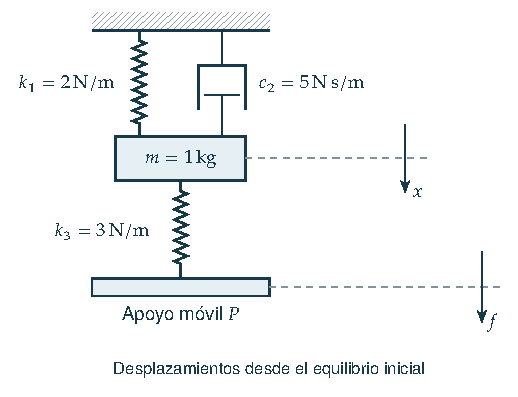
\includegraphics[width=9.83cm]{assets/M2-E0129-setup.pdf}\par
\smallskip{\small Conexiones de la masa con el soporte fijo y el apoyo móvil.\par}
\end{minipage}
\end{center}

\supportlinks{M2-E0129}{0}{0}
\exercise{M2-E0289}{Core · Intermedio}
Use Laplace para resolver $y^{(4)}-y=0$, $y(0)=0$, $y'(0)=1$, $y''(0)=0$, $y^{(3)}(0)=0$, para $t\ge0$.

\supportlinks{M2-E0289}{0}{0}
\exercise{M2-E0040}{Core · Intermedio}
Calcular las siguientes transformadas inversas unilaterales como funciones causales para \(t\ge0\). Usar \(H(t)=0\) si \(t<0\) y \(H(t)=1\) si \(t\ge0\); se identifican funciones que sólo difieren en valores aislados.

\begin{enumerate}[label=(\alph*),ref=\alph*,leftmargin=*]
\item (a) \(F(s)=\frac1{s-4}\).
\item (b) \(F(s)=\frac1{(s-4)^3}\).
\item (c) \(F(s)=\frac{e^{-2s}}{(s-4)^3}\).
\item (d) \(F(s)=\frac{1-2e^{-2s}}{(s-4)^3}\).
\item (e) \(F(s)=\frac1{(s-3)(s+1)}\).
\item (f) \(F(s)=\frac{1-e^{-2s}}{(s-3)(s+1)}\).
\item (g) \(F(s)=\frac1{s^3-s^2-s+1}\).
\item (h) \(F(s)=\frac{s+3}{(s+1)^2+4}\).
\item (i) \(F(s)=\frac{1-2e^{-2s}}{s(s-4)}\).
\item (j) \(F(s)=\frac1{(s-4)(1+e^{-s})}\).
\item (k) \(F(s)=\frac1{(s^2+1)(1-2e^{-3s})}\).
\end{enumerate}

\supportlinks{M2-E0040}{0}{0}
\chapter{Sistemas acoplados y evolución de varias cantidades}
\label{chapter:7}
%
\subsection*{Estados y sistemas equivalentes}
\label{CH07-B01}
Una EDO de segundo orden $y''=f(t,y,y')$ se escribe como
$x_1'=x_2$, $x_2'=f(t,x_1,x_2)$, con $x_1=y$, $x_2=y'$ y ambos
datos iniciales. El producto matriz-vector se calcula por filas:
$(A\mathbf x)_i=\sum_j a_{ij}x_j$.

Eliminar una componente puede producir una EDO escalar, pero la
equivalencia exige reconstruirla con las mismas constantes y comprobar
todo el sistema. Las condiciones iniciales de la ecuación eliminada
proceden del sistema original. Si éste tiene forma
$B\mathbf x'=A\mathbf x+\mathbf f$, sólo puede despejarse
$\mathbf x'$ mediante $B^{-1}$ cuando $B$ es invertible. Una matriz
$B$ singular puede imponer una relación algebraica entre estados y datos.
Recuérdense sistemas lineales y determinantes.
Consulta: solución de \exref{M2-E0238}.

%
\subsection*{Evolución lineal y autovectores}
\label{CH07-B02}
En $\mathbf x'=A\mathbf x$, con $A$ constante, un autovector no nulo
$\mathbf v$ de autovalor $\lambda$ produce
$e^{\lambda t}\mathbf v$. Calcúlense los autovalores con
$\det(A-\lambda I)=0$ y los autovectores resolviendo
$(A-\lambda I)\mathbf v=0$. Para una matriz real, las partes real e
imaginaria de un modo complejo conjugado dan soluciones reales.

Una raíz repetida no garantiza suficientes autovectores independientes.
En el caso concreto $A=\lambda I+N$, $N^2=0$, se puede comprobar por
derivación que
\[
 \mathbf x(t)=e^{\lambda(t-t_0)}
 [I+(t-t_0)N]\mathbf x(t_0).
\]
Para $\mathbf x'=A\mathbf x+\mathbf f(t)$, la solución es homogénea
más particular. Una entrada constante sugiere una particular constante
sólo si $A\mathbf x_p+\mathbf f=0$ es compatible; otras entradas
pueden requerir otro ensayo. Verifíquense todas las componentes y datos.
Consultas: soluciones de \exref{M2-E0047} y \exref{M2-E0065}.

%
\subsection*{Balances, reducción y observación}
\label{CH07-B03}
Escríbase un balance por cada cantidad almacenada. En una mezcla,
$Q_i=V_i c_i$; si cambia $V_i$, también interviene $V_i'c_i$.
Al sumar balances, los intercambios internos se cancelan y quedan los
intercambios con el exterior y las fuentes o consumos. Que aumente una
componente no implica que aumente el total.

Las variables suma y diferencia pueden separar evolución conjunta y
desequilibrio. Para justificar que dos estados permanecen iguales,
compruébese que sus derivadas coinciden cuando los estados coinciden;
con datos iguales y unicidad, esa igualdad se conserva. No basta imponerla
en una sola ecuación. Distínganse el estado físico, la salida de un sensor
$H(\mathbf x)$ y un registro acumulado
$z'=H(\mathbf x)$: miden objetos distintos y pueden tener unidades
distintas. Consulta: solución de \exref{M2-E0343}.

%
\subsection*{Etapas vectoriales y límites de la aproximación}
\label{CH07-B04}
Euler, Heun y RK4 se aplican a $\mathbf x'=\mathbf f(t,\mathbf x)$
con las mismas fórmulas del capítulo 3, sustituyendo números por vectores.
Cada etapa utiliza todas las componentes del mismo estado provisional;
actualizar una componente y usarla de inmediato para calcular otra cambia
el método.

Compruébense invariantes, signos, unidades y balances. Conservar una suma
no garantiza aproximar bien cada componente. Las primeras etapas manuales
permiten entender el algoritmo; cuando se pide una malla larga, puede usarse
la ayuda de cálculo de esta edición para las repeticiones.
La concordancia entre mallas es evidencia numérica, no una tolerancia
certificada ni una validación empírica de las leyes. Para una decisión
garantizada, búsquense cotas justificadas mediante balances y
desigualdades, e indíquense las hipótesis del modelo.
Consultas: soluciones de \exref{M2-E0315} y \exref{M2-E0362}.

\Needspace{12\baselineskip}
\section{Estados y descripciones equivalentes}
\exercise{M2-E0290}{Core · Básico}
Convierta $y^{(4)}+3y''-2y'+4y=2e^{3t}$ en un sistema de primer orden y escriba su forma matricial.

\supportlinks{M2-E0290}{0}{0}
\exercise{M2-E0238}{Core · Básico}
Resuelva el sistema de primer orden reduciéndolo a una ecuación de orden mayor:
\[x_1'=x_1+2x_2,\qquad x_2'=-2x_1+x_2,\qquad t\in\mathbb R.\]

\supportlinks{M2-E0238}{1}{0}
\exercise{M2-E0064}{Core · Básico}
Resolver por reducción
\[x_1'=2x_1+x_2-3,\qquad x_2'=-x_2+2e^t.\]

\supportlinks{M2-E0064}{0}{0}
\exercise{M2-E0059}{Core · Intermedio}
Resolver por reducción a una ecuación diferencial, para \(t\in\mathbb R\),
\[x_1'=-4(x_1+x_2),\qquad x_1'+4x_2'=-4x_2.\]

\supportlinks{M2-E0059}{0}{0}
\exercise{M2-E0344}{Core · Intermedio}
En un modelo determinista de circulación, las cantidades \(x\) e \(y\) en dos estados A y B se transfieren en ambos sentidos con la misma tasa \(k=1\,\mathrm{min}^{-1}\):
\[
x'=-kx+ky,\qquad y'=kx-ky.
\]
Se comparan dos preparaciones sintéticas, P con \((x(0),y(0))=(8,2)\) y Q con \((2,8)\). Un monitor informa de la cantidad total \(x+y\). Se puede guardar además uno de estos registros: un contador que reúne los traslados en ambos sentidos, o un contador que conserva sólo los traslados de A a B.

Los contadores empiezan en cero en cada ensayo y acumulan las integrales de las tasas de traslado; no son recuentos aleatorios. Un elemento puede trasladarse y contarse varias veces. Para una duración \(T>0\), determine qué información permiten distinguir el monitor total y cada contador, y decida qué registro adicional conserva la diferencia entre P y Q.

Compare también el límite de la diferencia entre sus cantidades instantáneas con el límite de la diferencia entre sus contadores direccionales cuando \(T\) aumenta. Distinga una diferencia histórica finita del valor de un contador que sigue acumulando eventos.

\supportlinks{M2-E0344}{0}{0}
\Needspace{12\baselineskip}
\section{Evolución lineal y balances}
\exercise{M2-E0047}{Core · Intermedio}
Dos tanques A y B contienen inicialmente 100 litros de salmuera cada uno, con 5 kg de sal
en A y 2 kg en B. Desde \(t=0\), entra agua pura en A a 6 L/min; pasan 8 L/min de A a B,
2 L/min de B a A y salen 6 L/min de B al exterior. La mezcla de cada tanque se mantiene
uniforme. Determinar la cantidad de sal en cada tanque para \(t\ge0\).

\Needspace{4.8cm}
\begin{center}
\begin{minipage}{\linewidth}
\centering
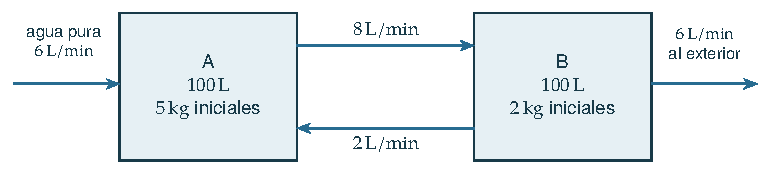
\includegraphics[width=14.62cm]{assets/M2-E0047-setup.pdf}\par
\smallskip{\small Caudales suministrados y cantidades iniciales en los dos tanques.\par}
\end{minipage}
\end{center}

\supportlinks{M2-E0047}{1}{0}
\exercise{M2-E0060}{Core · Intermedio}
Resolver por reducción
\[x_1'=8x_2,\qquad x_2'=-2x_3,\qquad x_3'=2x_1+8x_2-2x_3.\]

\supportlinks{M2-E0060}{0}{0}
\exercise{M2-E0046}{Core · Intermedio}
Resolver el problema de valor inicial
\[\binom{x_1'}{x_2'}=\begin{pmatrix}1&1\\1&1\end{pmatrix}\binom{x_1}{x_2}
+\binom{1+\sin(2t)}{1-\sin(2t)},\qquad X(0)=\binom01.\]

\supportlinks{M2-E0046}{0}{0}
\exercise{M2-E0065}{Core · Avanzado}
Resolver matricialmente los siguientes sistemas homogéneos.

\begin{enumerate}[label=(\alph*),ref=\alph*,leftmargin=*]
\item Resolver \(X'=AX\) para \(A=\begin{pmatrix}-2&-5\\1&2\end{pmatrix}\).
\item Resolver \(X'=AX\) para \(A=\begin{pmatrix}0&1&1\\3&0&1\\3&1&0\end{pmatrix}\).
\item Resolver \(X'=AX\) para \(A=\begin{pmatrix}3&1&-1\\1&3&-1\\3&3&-1\end{pmatrix}\).
\item Resolver \(X'=AX\) para \(A=\begin{pmatrix}4&3&1\\-4&-4&-2\\8&12&6\end{pmatrix}\).
\end{enumerate}

\supportlinks{M2-E0065}{1}{0}
\exercise{M2-E0291}{Core · Intermedio}
Resuelva por reducción el sistema $x_1'=2x_1-x_2+3t$, $x_2'=-x_1+x_2$.

\supportlinks{M2-E0291}{0}{0}
\exercise{M2-E0062}{Core · Intermedio}
Resolver por reducción
\[x_1'+x_2=t^2,\qquad x_2'-x_1=1.\]

\supportlinks{M2-E0062}{0}{0}
\exercise{M2-E0070}{Core · Intermedio}
Dos masas cuelgan en serie de un soporte fijo: el resorte \(k_1\) une el soporte a \(m_1\)
y el resorte \(k_2\) une \(m_1\) a \(m_2\). Sean
\[m_1=1\ \mathrm{kg},\quad m_2=1.25\ \mathrm{kg},\quad k_1=k_2=100\ \mathrm{N/m}.\]
Determinar las frecuencias naturales de las pequeñas oscilaciones verticales sin amortiguamiento,
medidas desde el equilibrio estático.

\Needspace{8.14cm}
\begin{center}
\begin{minipage}{\linewidth}
\centering
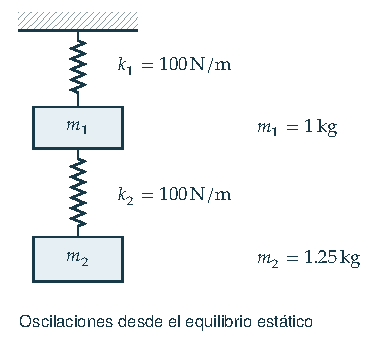
\includegraphics[width=7.21cm]{assets/M2-E0070-setup.pdf}\par
\smallskip{\small Conexión en serie de los dos muelles y las dos masas.\par}
\end{minipage}
\end{center}

\supportlinks{M2-E0070}{0}{0}
\exercise{M2-E0066}{Core · Avanzado}
Resolver por el método matricial.

\begin{enumerate}[label=(\alph*),ref=\alph*,leftmargin=*]
\item \[x_1'=x_2,\qquad x_2'=8x_1-2x_2+e^t.\]
\item \[x_1'=x_2,\qquad x_2'=-9x_1+6x_2+t.\]
\end{enumerate}

\supportlinks{M2-E0066}{0}{0}
\exercise{M2-E0067}{Core · Intermedio}
Resolver
\[x_1'=2x_1+x_2+2e^t,\qquad x_2'=-3x_1-2x_2+4e^t.\]

\supportlinks{M2-E0067}{0}{0}
\Needspace{12\baselineskip}
\section{Conservación, cálculo y reducción}
\exercise{M2-E0342}{Core · Básico}
En un modelo sintético, una población normalizada se divide en fracciones susceptible \(S\), activa \(I\) y retirada \(R\). Sólo se producen transferencias de \(S\) a \(I\), a tasa \(2SI\), y de \(I\) a \(R\), a tasa \(I\). Con \(t\) en días, los dos estados que se calculan satisfacen
\[
S'=-2SI,\qquad I'=2SI-I,
\qquad S(0)=0.8,\quad I(0)=0.1,\quad R(0)=0.1.
\]
Los coeficientes de las tasas tienen unidades \(\mathrm{día}^{-1}\).

Realice un paso de Heun de tamaño \(h=0.5\) días, formando el vector predictor completo antes de corregir sus componentes. Determine qué incremento debe registrar la fracción retirada si se usan las mismas dos evaluaciones de tasa y los mismos pesos de Heun. Relacione ese incremento con la disminución calculada de \(S+I\), y compruebe que los estados de este paso permiten esa interpretación como transferencias de fracciones.

\supportlinks{M2-E0342}{0}{0}
\exercise{M2-E0315}{Core · Intermedio}
En una simulación, dos cuerpos de temperaturas uniformes \(T_1,T_2\) intercambian calor entre sí y están aislados del exterior. Sus capacidades térmicas son \(C_1=2\,\mathrm{kJ/K}\) y \(C_2=3\,\mathrm{kJ/K}\). La potencia que pasa del primero al segundo es \(K(T_1-T_2)\), con \(K=1\,\mathrm{kJ/(min\,K)}\). Inicialmente están a \(80\) y \(20\,{}^\circ\mathrm C\).

Formule los balances y aplique un paso de Heun de \(h=0.6\,\mathrm{min}\). Use el trapecio explícito vectorial:
\[
\widetilde{\mathbf T}=\mathbf T_0+h\mathbf f(\mathbf T_0),\qquad
\mathbf T_1=\mathbf T_0+\frac h2[\mathbf f(\mathbf T_0)+\mathbf f(\widetilde{\mathbf T})].
\]
Identifique, a partir de los balances, una magnitud conservada y compruebe qué ocurre con ella en el predictor y en la corrección de Heun. Obtenga también una referencia analítica usando la diferencia de temperaturas y la conservación. Compare las temperaturas aproximadas con esa referencia y explique qué información aporta cada una de las dos comprobaciones: conservación y error de temperatura.

\supportlinks{M2-E0315}{1}{0}
\exercise{M2-E0048}{Core · Avanzado}
Dos tanques A y B contienen 100 L cada uno. Pasan 3 L/min de A a B y 1 L/min de B a A.
Entra en A una solución con 2 kg/L de sal a 6 L/min. Salen al exterior 4 L/min de A y
2 L/min de B. Inicialmente A contiene agua pura y B contiene 200 kg de sal.
Suponiendo mezcla uniforme y caudales constantes, determinar la sal contenida en cada tanque para \(t\ge0\).

\supportlinks{M2-E0048}{0}{0}
\exercise{M2-E0343}{Core · Avanzado}
Dos recintos bien mezclados de un taller contienen un aerosol trazador. Sus volúmenes constantes son \(V_1=50\) y \(V_2=100\,\mathrm{m^3}\). Circulan \(5\,\mathrm{m^3/min}\) en cada sentido entre ambos. Además, cada recinto recibe aire limpio del exterior y expulsa al exterior el mismo caudal: \(10\,\mathrm{m^3/min}\) el primero y \(20\,\mathrm{m^3/min}\) el segundo. Fuentes constantes añaden \(5\) y \(10\,\mathrm{mg/min}\), respectivamente.

Un limpiador sin intercambio neto de aire retira en el primer recinto una fracción \(k_1=0.10\,\mathrm{min}^{-1}\) de la cantidad de aerosol por unidad de tiempo. En el segundo, el coeficiente inicial es \(k_2=0\). No hay otras pérdidas. Los parámetros son sintéticos, y ambas concentraciones comienzan en \(0.20\,\mathrm{mg/m^3}\).

Formule los balances de cantidad y el sistema para las concentraciones \(c_1,c_2\). Determine si pueden representarse exactamente mediante una sola concentración común durante toda la evolución. Establezca qué condiciones sobre las fuentes y las tasas de eliminación por unidad de volumen harían válida esa reducción para cualquier concentración inicial común. Manteniendo los demás datos, determine qué valor de \(k_2\) la permitiría y escriba entonces la EDO para la concentración común.

\Needspace{9.17cm}
\begin{center}
\begin{minipage}{\linewidth}
\centering
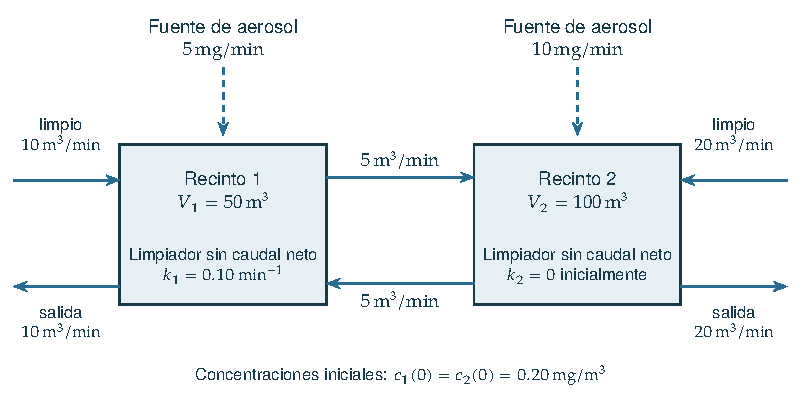
\includegraphics[width=15.18cm]{assets/M2-E0343-setup.pdf}\par
\smallskip{\small Ventilación, fuentes de aerosol y limpieza interna de los dos recintos.\par}
\end{minipage}
\end{center}

\supportlinks{M2-E0343}{1}{0}
\exercise{M2-E0063}{Core · Avanzado}
Resolver por reducción
\[\begin{aligned}x_1'&=2x_1+x_2-2x_3-t+2,\\x_2'&=1-x_1,\\x_3'&=x_1+x_2-x_3-t+1.\end{aligned}\]

\supportlinks{M2-E0063}{0}{0}
\exercise{M2-E0061}{Core · Avanzado}
Resolver por reducción el sistema implícito
\[x_1'+x_2'+2x_1=0,\qquad x_1'+x_2'-x_1-x_2=\sin t.\]

\supportlinks{M2-E0061}{0}{0}
\Needspace{12\baselineskip}
\section{Modelos y decisiones acumulativas}
\exercise{M2-E0369}{Core · Intermedio}
Un módulo industrial consta de una placa metálica y una carcasa en contacto. Ambas pueden almacenar calor y cederlo al aire. Un calefactor actúa sobre la placa; al apagarlo, una prueba sintética registra \(80\,{}^\circ\mathrm C\) en la placa y \(20\,{}^\circ\mathrm C\) en la carcasa, en aire a \(20\,{}^\circ\mathrm C\). Después sólo se registra un termómetro adherido a la carcasa. No hay cambios de fase. Almacenar una energía \(C\,\Delta T\) eleva la temperatura de una parte en \(\Delta T\), si su capacidad térmica \(C\) se considera constante.

Proponga un modelo diferencial que permita interpretar ese registro. Decida qué temperaturas necesita representar, qué intercambios conserva y cómo los describe. Declare las condiciones iniciales y los parámetros que habría que conocer. Resuelva un caso sencillo que usted justifique, compruebe su comportamiento límite y explique cuándo sería aceptable reemplazarlo por un modelo más simple. Señale una observación que ayude a decidir entre ambas descripciones.

\supportlinks{M2-E0369}{0}{0}
\exercise{M2-E0049}{Core · Avanzado}
El modelo suministrado para presas \(x_1\) y depredadores \(x_2\) es
\[x_1'=\alpha x_1-\beta x_1x_2,\qquad x_2'=\gamma x_1x_2-\delta x_2.\]
Con \(x_1(0)=1\), \(x_2(0)=3\), \(\alpha=\beta=2\) y \(\gamma=\delta=1\),
aproximar las poblaciones en \(t=1\) mediante Runge--Kutta clásico de cuarto orden,
usando \(h=0.025\).

\supportlinks{M2-E0049}{0}{0}
\exercise{M2-E0069}{Core · Avanzado}
Resolver
\[X'=\begin{pmatrix}3&-2&1\\2&-1&1\\-4&4&1\end{pmatrix}X+e^t\begin{pmatrix}t^2\\t\\1\end{pmatrix}.\]

\supportlinks{M2-E0069}{0}{0}
\exercise{M2-E0371}{Core · Intermedio}
En un proceso idealizado \(A\to B\to P\), las fracciones cumplen
\[
a'=-\alpha a,\qquad b'=\alpha a-\beta b,\qquad p'=\beta b,
\qquad (a,b,p)(0)=(1,0,0),\qquad \alpha,\beta>0.
\]
Con \(t\) expresado en minutos, un registro sintético del producto se trata como exacto:
\[
p(t)=1-3e^{-2t}+2e^{-3t},\qquad t\ge0.
\]
Determine qué se puede inferir sobre las tasas y si ese registro permite decidir cuál de las dos etapas es más lenta. Después se mide la fracción intermedia en \(t=\log2\) min: el instrumento indica \(0.30\), con error absoluto garantizado no mayor que \(0.06\). Decida qué añade esta lectura, manteniendo separado lo que depende del modelo de lo que permite la precisión del dato.

\supportlinks{M2-E0371}{0}{0}
\exercise{M2-E0359}{Core · Avanzado}
Un reactor idealizado contiene \(1\,\mathrm L\) de mezcla a temperatura constante. Antes de dosificar hay \(3\,\mathrm{mol}\) de A y no hay B ni P. La única reacción es \(\mathrm{A+B\longrightarrow P}\), con estequiometría uno a uno. La velocidad volumétrica de formación de P es \(k c_Ac_B\), donde \(c_A,c_B\) son las concentraciones y \(k=1\,\mathrm{L/(mol\,min)}\). Los datos son sintéticos.

Se comparan dos programas que añaden en total \(2\,\mathrm{mol}\) de B:
\[
\begin{array}{c|cc}
\text{programa}&t=0&t=0.5\,\mathrm{min}\\\hline
\mathrm I&2\,\mathrm{mol}&0\\
\mathrm{II}&1\,\mathrm{mol}&1\,\mathrm{mol}
\end{array}
\]
Las adiciones se idealizan como instantáneas, de volumen despreciable y mezcla inmediata. Durante el instante de adición sólo cambia la cantidad de B por la dosis indicada; la reacción avanza entre adiciones. No hay salida ni otras reacciones.

Se requiere obtener al menos \(1.40\,\mathrm{mol}\) de P al cabo de un minuto y mantener la cantidad de B libre por debajo o igual a \(1.50\,\mathrm{mol}\) en toda la operación, también inmediatamente después de cada carga. Formule los balances y las condiciones de unión, compare el producto obtenido y el máximo de B para cada programa, y decida cuáles cumplen los criterios. Explique por qué la fecha de evaluación importa al comparar dosis totales iguales. Puede usar calculadora.

\supportlinks{M2-E0359}{0}{0}
\exercise{M2-E0068}{Core · Avanzado · Representación}
Se suministra el PVI
\[y^{(3)}+yy''=(y')^2-1,\qquad y(0)=y'(0)=0,\quad y''(0)=1.32824.\]
Aproximar la solución y trazar su gráfica en \([0,2]\) mediante Euler explícito.
Para fijar una respuesta reproducible, utilizar \(h=0.1\); comparar con \(h=0.05\) y \(0.025\).

\supportlinks{M2-E0068}{0}{0}
\exercise{M2-E0045}{Core · Avanzado}
Resolver, según los valores reales de \(a\), el sistema \(X'=AX\), donde
\[A=\begin{pmatrix}0&1&0\\a&a-1&0\\-a&1-a&1\end{pmatrix}.\]

\supportlinks{M2-E0045}{0}{0}
\exercise{M2-E0362}{Core · Reto}
Un ensayo de filtración por gravedad comienza con \(1\,\mathrm L\) de suspensión homogénea sobre un filtro limpio. Sea \(V\) el volumen de líquido que queda en el depósito y \(m\) la masa de sólido depositada en el filtro. Se adoptan estas leyes idealizadas, con constantes sintéticas:
\[
\Delta p=\left(1\,\frac{\mathrm{kPa}}{\mathrm L}\right)V,
\qquad R=R_0+\beta m,
\qquad Q=\frac{\Delta p}{R},
\]
\[
R_0=1\,\frac{\mathrm{kPa}\,\mathrm{min}}{\mathrm L},
\qquad \beta=1\,\frac{\mathrm{kPa}\,\mathrm{min}}{\mathrm L\,\mathrm g}.
\]
Aquí \(Q\) es el caudal de filtrado. La suspensión que alcanza el filtro contiene siempre \(1\,\mathrm{g/L}\) de sólido, que queda retenido por completo. Un rascador retira del depósito sobre el filtro una fracción por minuto dada por \(\lambda=1\,\mathrm{min^{-1}}\): su caudal másico de retirada es \(\lambda m\). El sólido retirado va a un colector separado y lleva un volumen despreciable de líquido. No hay alimentación ni retorno. Se desprecian el volumen del sólido y cualquier retención adicional de líquido; por ello el volumen de filtrado recogido es la disminución de \(V\).

El ensayo dura \(0.5\,\mathrm{min}\). Se desea recoger al menos \(0.38\,\mathrm L\), manteniendo durante todo el ensayo \(V\ge0.60\,\mathrm L\) y \(m\le0.40\,\mathrm g\). Construya el modelo y decida si cumple los tres requisitos mediante cotas justificadas para la evolución. Obtenga también una estimación numérica breve del volumen recogido, indicando el método y el paso empleados, y distinga su alcance del de las cotas.

Como alternativa de diseño se ofrece un cartucho ideal que mantiene la resistencia \(R_0\) durante todo el ensayo, con las restantes leyes sin cambios. Determine si esta alternativa cambia la decisión. Puede usar calculadora; no se exige una fórmula cerrada para el sistema con resistencia variable.

\Needspace{9.46cm}
\begin{center}
\begin{minipage}{\linewidth}
\centering
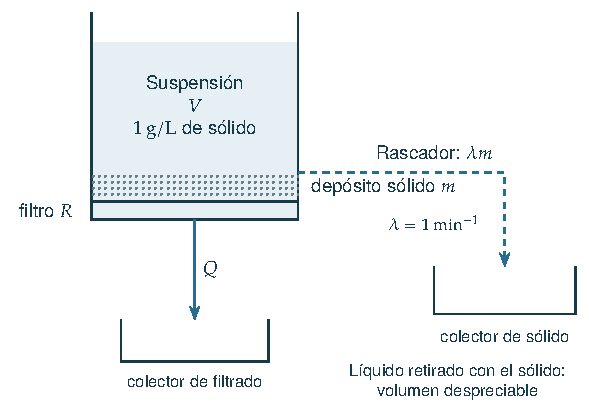
\includegraphics[width=11.17cm]{assets/M2-E0362-setup.pdf}\par
\smallskip{\small Rutas separadas del filtrado y del sólido retirado por el rascador.\par}
\end{minipage}
\end{center}

\supportlinks{M2-E0362}{1}{0}
\chapter{Ortogonalidad y series de Fourier}
\label{chapter:8}
%
\subsection*{Simetría y producto escalar}
\label{CH08-B01}
En un dominio simétrico, $f$ es par si $f(-x)=f(x)$ e impar si
$f(-x)=-f(x)$. Para funciones reales de cuadrado integrable, el producto
escalar y su norma son
\[
 \langle f,g\rangle=\int_{-L}^{L}f(x)g(x)\,dx,
 \qquad \|f\|^2=\langle f,f\rangle.
\]
Dos funciones son ortogonales cuando su producto escalar es cero.
Para $L>0$, la constante $1$, los cosenos y los senos de frecuencias
$n\pi/L$, $n\ge1$, son mutuamente ortogonales; sus normas al cuadrado
son $2L$, $L$ y $L$, respectivamente. Puede comprobarse con las
identidades de producto a suma, por ejemplo
$2\cos a\cos b=\cos(a-b)+\cos(a+b)$.
Una función impar integrable integra cero sobre $[-L,L]$.
Al comparar contribuciones a una aproximación importa el coeficiente
\emph{y} la norma de su función, no sólo el coeficiente.

%
\subsection*{Coeficientes, periodo y extensión}
\label{CH08-B02}
Para periodo $2L$, usamos la convención
\[
 f(x)\sim\frac{a_0}{2}+\sum_{n=1}^\infty
 \left[a_n\cos\frac{n\pi x}{L}+b_n\sin\frac{n\pi x}{L}\right],
\]
\[
 a_n=\frac1L\int_{-L}^{L}f(x)\cos\frac{n\pi x}{L}\,dx
 \ (n\ge0),\qquad
 b_n=\frac1L\int_{-L}^{L}f(x)\sin\frac{n\pi x}{L}\,dx.
\]
En una función par, $b_n=0$; en una impar, $a_n=0$. Para datos en
$(0,L)$, una extensión par da coeficientes de coseno mediante
$\frac2L\int_0^L f\cos(n\pi x/L)\,dx$; una impar da análogamente
coeficientes de seno. El observable físico decide la extensión: una
componente con signo y su módulo pueden tener simetrías distintas.
Compruébense periodo, frecuencia y unidades antes de integrar.
Consultas: soluciones de \exref{M2-E0051} y \exref{M2-E0345}.

Para interpretar un perfil que también depende del tiempo, una derivada
parcial mantiene fija la otra variable. En $u(x,t)=A(t)X(x)$,
$u_t=A'X$ y $u_{xx}=AX''$; sustituir en la ecuación dada permite obtener
una EDO de amplitud. Temperatura prescrita fija $u$; flujo nulo fija la
derivada espacial correspondiente cuando el flujo es proporcional a
$-u_x$. El desarrollo de estos modelos se recoge en el capítulo 10.

%
\subsection*{Suma de la serie y empalmes}
\label{CH08-B03}
Si la extensión periódica es suave a trozos, con límites laterales y un
número finito de piezas regulares por periodo, su serie de Fourier
converge en cada punto al promedio
\[
 \frac{f(x^-)+f(x^+)}{2}.
\]
En un punto de continuidad coincide con $f(x)$. En los extremos de un
periodo, los límites se leen usando el empalme periódico. Cambiar un
valor aislado no cambia los coeficientes. Una esquina continua no es un
salto del valor de la función.

La suma parcial hasta el armónico $N$ puede contener menos de $N$ términos
no nulos por simetría. Distíngase ese índice del número de componentes
retenidas. Cerca de un salto, el fenómeno de Gibbs produce oscilaciones
cuya zona se estrecha al aumentar $N$, sin desaparecer su sobreoscilación
relativa al salto. No se interprete una gráfica truncada como igualdad
puntual exacta.

%
\subsection*{Proyección y error cuadrático}
\label{CH08-B04}
Para una familia finita de funciones ortogonales no nulas $\phi_j$, la
mejor aproximación en el espacio que generan
respecto del error cuadrático usa
$c_j=\langle f,\phi_j\rangle/\|\phi_j\|^2$. En la convención anterior,
para $f$ de cuadrado integrable, Parseval da
\[
 \frac1L\int_{-L}^{L}|f|^2\,dx
 =\frac{a_0^2}{2}+\sum_{n\ge1}(a_n^2+b_n^2),\qquad
 \frac1L\int_{-L}^{L}|f-S_N|^2\,dx
 =\sum_{n>N}(a_n^2+b_n^2).
\]
Si $g$ es positiva y decreciente,
$\int_{N+1}^{\infty}g(x)\,dx\le\sum_{n>N}g(n)
\le\int_N^{\infty}g(x)\,dx$; compruébense esas hipótesis antes de
acotar una cola. La cota obtenida es integral, no uniforme ni puntual
cerca de un salto.

La media es $a_0/2$ y el promedio del cuadrado es
$a_0^2/4+\frac12\sum_{n\ge1}(a_n^2+b_n^2)$; su raíz es el valor
eficaz o media cuadrática. Un periodo elegido puede ser múltiplo del mínimo: revísense las
frecuencias realmente presentes. Consulta: solución de \exref{M2-E0348}.

\Needspace{12\baselineskip}
\section{Paridad, productos escalares y normas}
\exercise{M2-E0071}{Core · Básico}
Determinar si cada función es par, impar o ninguna de las dos. Considerar su dominio real natural.

\begin{enumerate}[label=(\alph*),ref=\alph*,leftmargin=*]
\item \(f(x)=x^3+\sin2x\).
\item \(f(x)=\sin^2x\).
\item \(f(x)=(1-x^2)^{-1/2}\), con valores reales.
\item \(f(x)=\sin(x+1)\).
\item \(f(x)=e^{-x}\cos3x\).
\item \(f(x)=x^{1/5}\cos(x^2)\), con la raíz quinta real.
\end{enumerate}

\supportlinks{M2-E0071}{0}{0}
\exercise{M2-E0285}{Core · Básico}
Demuestre que $1,\cos x,\cos2x,\ldots$ son ortogonales en $[-\pi,\pi]$ para el producto escalar sin peso y calcule sus normas.

\supportlinks{M2-E0285}{0}{0}
\exercise{M2-E0084}{Core · Básico}
Demostrar que cada pareja es ortogonal en el intervalo indicado con el producto escalar integral sin peso.

\begin{enumerate}[label=(\alph*),ref=\alph*,leftmargin=*]
\item \(f_1=x,f_2=x^2\), en \([-2,2]\).
\item \(f_1=x^3,f_2=x^2+1\), en \([-1,1]\).
\item \(f_1=e^x,f_2=(x-1)e^{-x}\), en \([0,2]\).
\item \(f_1=\cos x,f_2=\sin^2x\), en \([0,\pi]\).
\item \(f_1=x,f_2=\cos2x\), en \([-\pi/2,\pi/2]\).
\item \(f_1=e^x,f_2=\sin x\), en \([\pi/4,5\pi/4]\).
\end{enumerate}

\supportlinks{M2-E0084}{0}{0}
\exercise{M2-E0074}{Core · Básico}
Calcular la serie de Fourier de \(f(x)=\sin^2x\) en \((-\pi/2,\pi/2)\).

\supportlinks{M2-E0074}{0}{0}
\Needspace{12\baselineskip}
\section{Coeficientes y extensión periódica}
\exercise{M2-E0051}{Core · Básico}
Calcular la serie de Fourier de \(f(x)=|x|\) en \(-1<x<1\), con extensión de período 2.

\supportlinks{M2-E0051}{1}{0}
\exercise{M2-E0293}{Core · Básico}
Calcule la serie de Fourier $2\pi$-periódica de $f(x)=-1$ para $-\pi<x<0$ y $f(x)=1$ para $0<x<\pi$. Compare las sumas con1,2,3 y10 términos no nulos.

\supportlinks{M2-E0293}{0}{0}
\exercise{M2-E0050}{Core · Intermedio}
Calcular la serie de Fourier de \(f(x)=e^x\), \(-\pi<x<\pi\),
entendida con período \(2\pi\).

\supportlinks{M2-E0050}{0}{0}
\exercise{M2-E0346}{Core · Básico}
Una señal real, continua a trozos y de periodo \(2\pi\), satisface
\[
f(t+\pi)=-f(t)\qquad\text{para todo }t.
\]
En la convención
\[
f(t)\sim\frac{a_0}{2}+\sum_{n=1}^{\infty}
\bigl(a_n\cos nt+b_n\sin nt\bigr),
\]
determine qué coeficientes tienen que ser cero por esa relación. Justifique la respuesta sin calcular una señal concreta. Decida además si la relación obliga a que \(f\) sea impar respecto de \(t=0\) y si obliga a que \(2\pi\) sea su menor periodo positivo; use ejemplos breves cuando una conclusión no sea obligatoria.

\supportlinks{M2-E0346}{0}{0}
\exercise{M2-E0072}{Core · Intermedio}
Sea \(f\) de período2, definida por
\[f(x)=\begin{cases}0,&-1<x<0,\\1,&0<x<1.\end{cases}\]
Calcular su serie de Fourier. Los valores aislados en los puntos de salto no afectan a los coeficientes.

\supportlinks{M2-E0072}{0}{0}
\exercise{M2-E0052}{Core · Intermedio}
Considerar \(f(x)=x^2\), \(-\pi<x<\pi\), y su extensión periódica de período \(2\pi\).

\begin{enumerate}[label=(\alph*),ref=\alph*,leftmargin=*]
\item Demostrar que su serie de Fourier es
\[\frac{\pi^2}{3}+4\sum_{n=1}^{\infty}\frac{(-1)^n}{n^2}\cos nx.\]
\item Usar el apartado anterior y la convergencia de Fourier para demostrar
\(\sum_{n=1}^{\infty}(-1)^{n+1}/n^2=\pi^2/12\).
\item Usar el apartado (a) y la convergencia de Fourier para demostrar
\(\sum_{n=1}^{\infty}1/n^2=\pi^2/6\).
\end{enumerate}

\supportlinks{M2-E0052}{0}{0}
\Needspace{12\baselineskip}
\section{Medio intervalo y condiciones}
\exercise{M2-E0083}{Core · Intermedio}
Calcular la serie senoidal de Fourier de cada función.

\begin{enumerate}[label=(\alph*),ref=\alph*,leftmargin=*]
\item \(f(x)=-1\), \(0<x<1\).
\item \[f(x)=\begin{cases}x,&0<x\le\pi/2,\\\pi-x,&\pi/2\le x<\pi.\end{cases}\]
\item \(f(x)=x-x^2\), \(0<x<1\).
\end{enumerate}

\supportlinks{M2-E0083}{0}{0}
\exercise{M2-E0345}{Core · Intermedio}
En la mitad derecha de un montaje sobre una guía recta, \(0\le x\le L\), la componente de fuerza medida sobre un eje global orientado hacia la derecha es
\[
F_+(x)=F_0\frac{x}{L}\left(1-\frac{x}{L}\right),
\qquad F_0,L>0.
\]
Todas las fuerzas son paralelas a la guía. La mitad izquierda se obtiene por reflexión geométrica: se reflejan tanto las posiciones como las flechas de fuerza. El eje global usado para asignar el signo de la lectura se mantiene fijo. El patrón completo se repite con longitud espacial \(2L\).

Un instrumento informa de esa componente con signo, \(F(x)\), y otro del módulo de la fuerza, \(M(x)\). Construya ambas extensiones al periodo completo y elija para cada registro una serie de senos, de cosenos o completa en las frecuencias \(n\pi/L\), justificándolo desde la regla física. Calcule la media espacial de cada registro y sólo el primer coeficiente no nulo del registro con signo, en la convención usual \(a_0/2+\sum_{n\ge1}(a_n\cos(n\pi x/L)+b_n\sin(n\pi x/L))\).

\supportlinks{M2-E0345}{1}{0}
\exercise{M2-E0053}{Core · Intermedio}
Calcular la serie de Fourier en cosenos de las funciones indicadas en cada apartado.
Se utiliza en cada caso la extensión par y periódica del intervalo dado.

\begin{enumerate}[label=(\alph*),ref=\alph*,leftmargin=*]
\item \(f(x)=e^x\), \(0<x<1\).
\item \(f(x)=\sin x\), \(0<x<\pi\).
\item \(f(x)=0\) si \(0<x<1\), \(f(x)=1\) si \(1<x<2\), y \(f(x)=0\) si \(2<x<3\).
\item \(f(x)=2x+1\), \(0\le x\le3\).
\end{enumerate}

\supportlinks{M2-E0053}{0}{0}
\exercise{M2-E0354}{Core · Básico}
Una barra idealizada ocupa \(0\le x\le L\), con \(L>0\). La temperatura en exceso \(u\) cumple \(u_t=\kappa u_{xx}\), donde \(\kappa>0\) tiene unidades de longitud al cuadrado por unidad de tiempo. El extremo izquierdo se mantiene a la temperatura de referencia y el derecho está aislado; el flujo es proporcional a \(-u_x\).

Se quiere representar \(u\) mediante dos funciones espaciales, con amplitudes temporales independientes. Elija cuál de estas parejas respeta las condiciones físicas para cualquier valor de ambas amplitudes:
\[
\begin{array}{c|cc}
\mathrm A&\sin(\pi x/L)&\sin(2\pi x/L)\\
\mathrm B&\cos(\pi x/(2L))&\cos(3\pi x/(2L))\\
\mathrm C&\sin(\pi x/(2L))&\sin(3\pi x/(2L))
\end{array}
\]
Justifique la elección. Si las dos amplitudes elegidas parten de un mismo valor \(U_0>0\), determine qué fracción de su valor inicial conserva la segunda cuando la primera se ha reducido a la mitad. Interprete la diferencia mediante la ecuación de calor.

\supportlinks{M2-E0354}{0}{0}
\Needspace{12\baselineskip}
\section{Perfiles y aproximaciones}
\exercise{M2-E0292}{Core · Intermedio · Representación}
Calcule la serie de Fourier de $f(x)=x$ en $-1<x<1$, extendida con período2, y compare gráficamente las sumas de los primeros10 y300 términos.

\supportlinks{M2-E0292}{0}{0}
\exercise{M2-E0082}{Core · Intermedio}
Determinar la función a la que converge la serie de Fourier de cada f en el intervalo indicado.
No es necesario calcular los coeficientes. Describir también los valores de la suma en los puntos de salto y empalme. La serie usa el período dado por la longitud del intervalo.

\begin{enumerate}[label=(\alph*),ref=\alph*,leftmargin=*]
\item \(f(x)=x\), \(-\pi<x<\pi\).
\item \(f(x)=|x|\), \(-\pi<x<\pi\).
\item \(f=1\) en(\ensuremath{-}2,0) y \(f=x\) en(0,2).
\item \(f=0\) en(\ensuremath{-}\ensuremath{\pi},0) y \(f=x^2\) en(0,\ensuremath{\pi}).
\item \(f(x)=x^2\), \(-1<x<1\).
\item \(f=x+\pi\) en(\ensuremath{-}\ensuremath{\pi},0) y \(f=x\) en(0,\ensuremath{\pi}).
\item \(f(x)=e^x\), \(-\pi<x<\pi\).
\item \[f(x)=\begin{cases}0,&-\pi<x<-\pi/2,\\-1,&-\pi/2<x<0,\\1,&0<x<\pi/2,\\0,&\pi/2<x<\pi.\end{cases}\]
\end{enumerate}

\supportlinks{M2-E0082}{0}{0}
\exercise{M2-E0347}{Core · Básico}
Se quiere representar
\[
f(t)=2+\cos t+\sqrt5\sin(3t)+\sqrt6\cos(5t)
\]
en \([-\pi,\pi]\) mediante una combinación \(g\) de, como máximo, dos funciones del conjunto
\[
\{1,\ \cos t,\ \sin(3t),\ \cos(5t)\}.
\]
Cada función utilizada cuesta una unidad de presupuesto, incluida la constante; los coeficientes de \(g\) se pueden elegir libremente. El criterio es minimizar el error cuadrático medio
\[
\mathcal E(g)=\frac1{2\pi}\int_{-\pi}^{\pi}|f(t)-g(t)|^2\,dt.
\]
Elija las dos funciones y sus coeficientes, calcule el error mínimo y justifique la optimalidad usando la ortogonalidad. El presupuesto cuenta funciones escalares, no parejas seno--coseno ni frecuencias completas.

\supportlinks{M2-E0347}{0}{1}
\exercise{M2-E0073}{Core · Intermedio}
Calcular la serie de Fourier de
\[f(x)=\begin{cases}0,&-\pi<x<0,\\x,&0<x<\pi,\end{cases}\]
para su extensión2\ensuremath{\pi}-periódica.

\supportlinks{M2-E0073}{0}{0}
\exercise{M2-E0305}{Core · Intermedio}
Para cada perfil, calcule los coeficientes de su extensión periódica de período $2L$ en la forma
\[
C+\sum_{n=1}^{\infty}\left[a_n\cos\left(\frac{n\pi x}{L}\right)+b_n\sin\left(\frac{n\pi x}{L}\right)\right].
\]
Antes de integrar, determine qué simplificaciones permiten las simetrías o las identidades trigonométricas. Indique también el valor al que converge la serie en los saltos y en los extremos del intervalo. Los valores que se asignen en puntos aislados no modifican los coeficientes.

\begin{enumerate}[label=(\alph*),ref=\alph*,leftmargin=*]
\item $L=2$, \quad $f(x)=\begin{cases}1-x^2,&|x|\leq1,\\0,&1<|x|<2.\end{cases}$
\item $L=3$, \quad $f(x)=\begin{cases}0,&|x|\leq1,\\x,&1<|x|<3.\end{cases}$
\item $L=2$, \quad $f(x)=|x-\tfrac12|$, \quad $-2<x<2$.
\item $L=1$, \quad $f(x)=x(1-x^2)$, \quad $-1<x<1$.
\item $L=\pi$, \quad $f(x)=(\cos x+\sin2x)^2$, \quad $-\pi<x<\pi$.
\item $L=\pi$, \quad $f(x)=x\sin x$, \quad $-\pi<x<\pi$.
\end{enumerate}

\supportlinks{M2-E0305}{0}{0}
\Needspace{12\baselineskip}
\section{Contrastes y síntesis}
\exercise{M2-E0349}{Core · Intermedio}
Se quieren construir señales reales mediante una constante y sólo los armónicos de índices \(2\) y \(3\) respecto de un periodo \(2\pi\). Los dos coeficientes del primer armónico deben ser cero. Se prescribe
\[
\frac1{2\pi}\int_0^{2\pi}f(t)\,dt=2,
\qquad
\frac1{2\pi}\int_0^{2\pi}f(t)^2\,dt=Q.
\]
La segunda cantidad es la media del cuadrado, no su raíz. La señal debe ser no constante y tener \(2\pi\) como menor periodo positivo.

Determine para qué valores de \(Q\) es posible la construcción. Describa las amplitudes y fases que quedan libres bajo esas condiciones, y exhiba una señal concreta para \(Q=5\). Justifique tanto los momentos prescritos como el periodo mínimo de la señal construida; no basta que \(2\pi\) sea uno de sus periodos.

\supportlinks{M2-E0349}{0}{0}
\exercise{M2-E0348}{Core · Avanzado}
Sea la señal \(2\pi\)-periódica definida en un periodo por
\[
f(t)=
\begin{cases}
-1,&-\pi\le t<0,\\
1,&0\le t<\pi.
\end{cases}
\]
Considere sus sumas de \(N\ge1\) armónicos impares,
\[
S_N(t)=\frac4\pi\sum_{j=0}^{N-1}
\frac{\sin((2j+1)t)}{2j+1},
\qquad
E_N=\frac1{2\pi}\int_{-\pi}^{\pi}|f(t)-S_N(t)|^2\,dt.
\]
Usando Parseval y una comparación de series positivas con integrales, exprese \(E_N\) como una cola y dé un número suficiente de términos para garantizar \(E_N\le0.01\). Contraste esa garantía con el error en \(t=0\). Explique qué cambiaría si se reasignara únicamente \(f(0)=0\), y si esa reasignación permitiría obtener un error uniformemente pequeño en un entorno que contenga puntos a ambos lados del salto.

\supportlinks{M2-E0348}{1}{0}
\chapter{Sturm–Liouville y expansiones en autofunciones}
\label{chapter:9}
%
\subsection*{Problema regular y parámetro espectral}
\label{CH09-B01}
Usamos la forma
\[
 -(p y')'+q y=\lambda w y\quad (a<x<b),
\]
con intervalo finito, $p$ de clase $C^1$, $q,w$ continuas y reales,
y $p,w>0$ en $[a,b]$. Se añaden condiciones homogéneas separadas
de valor, derivada o Robin; en cada extremo,
$\alpha y+\beta y'=0$, con constantes reales no simultáneamente nulas
e independientes de $\lambda$. Un autovalor admite una autofunción
\emph{no idénticamente nula}.

Al resolver, sepárense los casos $\lambda<0$, $\lambda=0$ y
$\lambda>0$ cuando den formas distintas de la EDO. La función constante
no nula puede ser un modo admisible; no debe confundirse con la función
nula. Tampoco cualquier condición de Robin garantiza autovalores
positivos. Recuérdense EDO lineales e integración por partes.
Consulta: solución de \exref{M2-E0054}.

%
\subsection*{Peso, normalización y expansión}
\label{CH09-B02}
El producto escalar correspondiente al problema es
$\langle f,g\rangle_w=\int_a^b wfg\,dx$.
Las autofunciones de autovalores distintos son ortogonales con este peso.
Con $N_n^2=\int_a^b w\phi_n^2\,dx$, la función normalizada es
$e_n=\phi_n/N_n$, y
\[
 f\sim\sum_n c_n\phi_n,\qquad
 c_n=\frac{\int_a^b wf\phi_n\,dx}{N_n^2}.
\]
En la base normalizada, el coeficiente es
$\langle f,e_n\rangle_w=c_nN_n$. Cambiar la normalización cambia los
coeficientes, pero no cada producto coeficiente por autofunción.

Para los problemas regulares y las bases completas aquí utilizadas,
la expansión converge en norma cuadrática ponderada para datos de
cuadrado integrable. Las afirmaciones puntuales necesitan regularidad
adicional. Una representación interior no impone automáticamente los
valores ni las derivadas del dato en los extremos; no se derive la serie
sin justificarlo. Consulta: solución de \exref{M2-E0297}.

%
\subsection*{Contornos físicos y cambio de medida}
\label{CH09-B03}
Si el flujo en la dirección positiva es $J=-k u_x$, con $k>0$, el
flujo saliente del intervalo es $-J(a)=k u_x(a)$ a la izquierda y
$J(b)=-k u_x(b)$ a la derecha. Esos signos deben introducirse antes de
traducir una ley de intercambio a una condición Robin.
Identifíquense $p,q,w$ en la ecuación escrita y compruébense las unidades
de $\lambda$; el peso no es un añadido de notación.

En un cambio monótono y regular $x=\chi(\xi)$, la medida también cambia:
\[
 \int w(x)f(x)g(x)\,dx
 =\int w(\chi(\xi))f(\chi(\xi))g(\chi(\xi))
        |\chi'(\xi)|\,d\xi,
\]
con los límites ordenados de menor a mayor en ambos intervalos.
Transformar las funciones sin el jacobiano puede destruir la
ortogonalidad. Revísense regularidad y positividad en todo el intervalo
cerrado, incluidos los extremos. Consultas: soluciones de
\exref{M2-E0350} y \exref{M2-E0351}.

%
\subsection*{Forzamiento, compatibilidad y límites}
\label{CH09-B04}
Con los mismos contornos homogéneos, escribamos
$-(py')'+qy-\lambda wy=wf$. Proyectar sobre un modo $\phi_n$ da
\[
 (\lambda_n-\lambda)c_n
 =\frac{\langle f,\phi_n\rangle_w}{\|\phi_n\|_w^2}.
\]
Si $\lambda=\lambda_n$, el miembro derecho debe anularse. En los
problemas regulares elementales tratados, con forzamiento regular, la
compatibilidad con el modo resonante permite resolver y deja libre su
coeficiente homogéneo. La resonancia puede dar inexistencia o no
unicidad: compruébese cuál ocurre, antes de calcular una particular.

Si los autovalores se obtienen como raíces, indíquese el intervalo y el
índice de cada raíz. Una aproximación relativa
$\lambda_n/\widetilde\lambda_n\to1$ no obliga al error absoluto a
tender a cero. En límites de familias, úsense cotas con el dominio y los
parámetros especificados; el problema límite puede conservar libertad
sin seleccionar una única solución. Consulta: solución de
\exref{M2-E0088}.

\Needspace{12\baselineskip}
\section{Contornos y modos}
\exercise{M2-E0316}{Core · Básico}
Considere
\[
-\big[(1+x)y'\big]'=\lambda(1+x)y,\qquad0<x<2,\qquad y'(0)=y'(2)=0.
\]
Una autofunción debe ser no idénticamente nula. Determine si \(\lambda=0\) admite autofunciones y describa todas las que correspondan a ese valor, sin buscar el espectro completo. Explique qué libertad queda en su amplitud después de imponer las condiciones de contorno. Si existe un modo para \(\lambda=0\), seleccione el que sea positivo y tenga norma uno para
\(\|y\|_w^2=\int_0^2(1+x)y(x)^2\,dx\).

\supportlinks{M2-E0316}{0}{1}
\exercise{M2-E0054}{Core · Intermedio}
Encontrar los autovalores reales y las autofunciones de \(y''+\lambda y=0\),
\(0<x<1\), con las condiciones de cada apartado. Se buscan autofunciones no idénticamente nulas.

\begin{enumerate}[label=(\alph*),ref=\alph*,leftmargin=*]
\item \(y'(0)=0,\ y(1)=0\).
\item \(y'(0)=0,\ y'(1)=0\).
\end{enumerate}

\supportlinks{M2-E0054}{1}{0}
\exercise{M2-E0353}{Core · Básico}
Se sabe que un problema espacial tiene la ecuación
\[
-X''=\lambda X,\qquad 0<x<L,
\]
con \(L>0\) conocido. En cada extremo se impone exactamente una de estas dos condiciones: valor nulo \(X=0\) o derivada nula \(X'=0\). Se desconoce cuál se usa en cada extremo.

Un registro sintético exacto contiene los dos menores autovalores \emph{estrictamente positivos}:
\[
\lambda_1^+=\left(\frac{\pi}{L}\right)^2,
\qquad \lambda_2^+=\left(\frac{2\pi}{L}\right)^2.
\]
El registro no ha comprobado si \(\lambda=0\) es autovalor. Determine todas las parejas de condiciones compatibles con la información disponible. ¿Bastaría comprobar la existencia de una autofunción de autovalor cero para identificar la pareja? Justifique ambas decisiones.

\supportlinks{M2-E0353}{0}{0}
\exercise{M2-E0297}{Core · Intermedio}
Desarrolle $f(x)=x$, $0<x<\pi$, en las autofunciones de $y''+\lambda y=0$, $y(0)=y(\pi)=0$. Determine la normalización e interprete la expansión en los extremos.

\supportlinks{M2-E0297}{1}{0}
\Needspace{12\baselineskip}
\section{Peso y normalización}
\exercise{M2-E0350}{Core · Intermedio}
Una barra idealizada de sección constante ocupa \(0\le x\le L\). Su temperatura en exceso respecto de un mismo ambiente constante es \(u(x,t)\). El flujo de calor por unidad de área, positivo hacia la derecha, y el balance local son
\[
q(x,t)=-k(x)u_x(x,t),\qquad c_0u_t=-q_x,
\qquad k(x)=k_0\left(1+\frac{x}{L}\right),
\]
con \(L,k_0,c_0>0\). En cada extremo, el flujo \emph{saliente} por unidad de área es proporcional al exceso de temperatura: el coeficiente es \(h_0>0\) a la izquierda y \(h_L>0\) a la derecha. Los coeficientes de transferencia tienen las unidades habituales de flujo por unidad de temperatura.

Traduzca estas leyes a las dos condiciones de contorno para \(u\), justificando sus signos con las direcciones salientes. Para una solución separada \(u(x,t)=X(x)e^{-\lambda t}\), formule después el problema para \(X\) en la convención
\[
-(pX')'+rX=\lambda wX.
\]
Identifique \(p,r,w\), compruebe la regularidad y positividad exigidas en todo el intervalo cerrado e indique las unidades de \(\lambda\).

\supportlinks{M2-E0350}{1}{0}
\exercise{M2-E0085}{Core · Intermedio}
Considerar
\[y''-2y'+(1+\lambda)y=0,\qquad y(0)=y(1)=0,\quad x\in[0,1],\quad \lambda\in\mathbb R.\]
Resolver los siguientes apartados.

\begin{enumerate}[label=(\alph*),ref=\alph*,leftmargin=*]
\item Introducir \(y=s(x)u\) y determinar s para eliminar el término en u\ensuremath{^{\prime}}.
\item Resolver el problema transformado y determinar los autovalores y autofunciones originales.
\item Resolver directamente sin introducir u.
\end{enumerate}

\supportlinks{M2-E0085}{0}{0}
\exercise{M2-E0351}{Core · Intermedio}
Considere
\[
x^2y''+xy'+\lambda y=0,\qquad 1<x<e,\qquad y(1)=y(e)=0,
\]
y los perfiles \(u(x)=\sin(\pi\log x)\), \(v(x)=\sin(2\pi\log x)\), donde \(\log\) es el logaritmo natural.

Escriba la ecuación como un problema regular de Sturm--Liouville e identifique su peso. Decida qué producto interno corresponde a la ortogonalidad de estos perfiles y calcule tanto
\[
\int_1^e u(x)v(x)\,dx
\qquad\text{como}\qquad
\int_1^e u(x)v(x)w(x)\,dx.
\]
Explique, mediante el cambio \(z=\log x\), por qué los dos resultados no tienen que coincidir.

\supportlinks{M2-E0351}{1}{0}
\exercise{M2-E0055}{Core · Avanzado}
Considerar el problema \(y''+\lambda y=0\), \(0<x<1\),
con \(y(0)=0\) y \(y'(1)=0\), y el producto escalar \(\langle f,g\rangle=\int_0^1fg\,dx\).

\begin{enumerate}[label=(\alph*),ref=\alph*,leftmargin=*]
\item Encontrar los autovalores y autofunciones.
\item Determinar las autofunciones normalizadas.
\item Desarrollar \(f(x)=1\) usando las autofunciones anteriores. Interpretar la igualdad en \(L^2(0,1)\) y los valores de la suma en los extremos.
\item Desarrollar en la base normalizada \(f(x)=2x\) si \(0\le x<1/2\), y \(f(x)=1\) si \(1/2\le x\le1\).
\end{enumerate}

\supportlinks{M2-E0055}{0}{0}
\Needspace{12\baselineskip}
\section{Espectros y parámetros}
\exercise{M2-E0239}{Core · Intermedio}
Halle los autovalores y las autofunciones no nulas de
\[y''+\lambda y=0,\qquad0<x<1,\qquad y(0)+y'(0)=0,\quad y(1)+y'(1)=0.\]

\supportlinks{M2-E0239}{0}{0}
\exercise{M2-E0087}{Core · Avanzado}
Considerar
\[y''+\lambda y=0,\qquad y'(0)=0,\quad y(1)+y'(1)=0,\quad 0\le x\le1.\]
Se emplea el producto escalar sin peso.

\begin{enumerate}[label=(\alph*),ref=\alph*,leftmargin=*]
\item Hallar las autofunciones normalizadas.
\item Desarrollar \(f(x)=1-x\) en \([0,1]\) en las autofunciones anteriores.
\item Desarrollar \(f(x)=1\) si \(0\le x<1/2\), y \(f(x)=0\) si \(1/2\le x\le1\).
\end{enumerate}

\supportlinks{M2-E0087}{0}{0}
\exercise{M2-E0241}{Core · Intermedio}
Se conocen los autovalores del problema
\[y''+\lambda y=0,\quad0<x<1,\quad y'(0)=0,\quad y(1)+y'(1)=0:\]
son $\lambda_n=\mu_n^2$, donde
\[\mu_n\tan\mu_n=1,\qquad(n-1)\pi<\mu_n<(n-1)\pi+\pi/2,\quad n\ge1.\]
Estime $\lambda_n$ para $n$ grande.

\supportlinks{M2-E0241}{0}{0}
\exercise{M2-E0086}{Core · Avanzado}
Sea \(\alpha\in\mathbb R\). Considerar
\[y''+\lambda y=0,\qquad \alpha y(0)+y'(0)=0,\quad y(1)=0.\]
Discutir el signo de sus autovalores según \ensuremath{\alpha}.

\begin{enumerate}[label=(\alph*),ref=\alph*,leftmargin=*]
\item Si \(\alpha<1\), demostrar que todos los autovalores son positivos.
\item Si \(\alpha=1\), demostrar que0 es autovalor.
\item Si \(\alpha>1\), demostrar que hay un único autovalor negativo, decreciente con \ensuremath{\alpha}, y que los demás son positivos.
\end{enumerate}

\supportlinks{M2-E0086}{0}{0}
\exercise{M2-E0240}{Core · Avanzado}
Para el problema
\[y''+\lambda y=0,\qquad0<x<\pi,\qquad y(0)=0,\quad y(\pi)+y'(\pi)=0,\]
encuentre las autofunciones y la ecuación de los autovalores, determine si $\lambda=0$ es autovalor y estime $\lambda_n$ para $n$ grande. Enumere los autovalores de menor a mayor, desde $n=1$.

\supportlinks{M2-E0240}{0}{0}
\Needspace{12\baselineskip}
\section{Contrastes y problemas de contorno}
\exercise{M2-E0056}{Core · Intermedio}
Hallar los valores reales de \(a\) para los que tiene solución
\[y''+\pi^2y=a,\quad0<x<1,\qquad y'(0)=y'(1)=0,\]
y encontrar las soluciones cuando existan.

\supportlinks{M2-E0056}{0}{0}
\exercise{M2-E0242}{Core · Avanzado}
Resuelva mediante un desarrollo en autofunciones
\[y''+2y=-x,\qquad0<x<1,\qquad y(0)=0,\quad y(1)+y'(1)=0.\]
Use el producto escalar sin peso en $[0,1]$.

\supportlinks{M2-E0242}{0}{0}
\exercise{M2-E0088}{Core · Intermedio}
Hallar los valores reales de a para los que tiene solución el problema
\[y''+\pi^2y=a-\cos\pi x,\qquad y(0)=y(1)=0.\]
Encontrar todas las soluciones en esos casos.

\supportlinks{M2-E0088}{1}{0}
\exercise{M2-E0243}{Core · Avanzado}
Resuelva mediante un desarrollo en autofunciones
\[y''+2y=-1+|1-2x|,\qquad0<x<1,\qquad y(0)=y(1)=0.\]
Use el producto escalar sin peso en $[0,1]$.

\supportlinks{M2-E0243}{0}{0}
\exercise{M2-E0089}{Core · Intermedio}
Determinar los autovalores reales y sus autofunciones no nulas del problema
\[y''+y'+\lambda(y'+y)=0,\qquad y'(0)=0,\quad y(1)=0.\]

\supportlinks{M2-E0089}{0}{0}
\exercise{M2-E0244}{Core · Avanzado}
Resuelva en $[0,1]$ el problema
\[y''+y=h(x),\qquad y'(0)=y'(1)=0,\qquad h(x)=\begin{cases}\tfrac12-x,&0\le x<\tfrac12,\\0,&\tfrac12\le x\le1.\end{cases}\]

\supportlinks{M2-E0244}{0}{0}
\exercise{M2-E0352}{Core · Avanzado}
Para \(0<\delta<1\), sea \(y_{\delta,\varepsilon}\) la solución del problema
\[
-y''=(1-\delta)y+\sin(2x)+\varepsilon\sin x,
\qquad 0<x<\pi,\qquad y(0)=y(\pi)=0.
\]
Se consideran dos familias de datos: \(\varepsilon=\delta\) y \(\varepsilon=\delta^2\). En ambas, \(\delta\) tiende a cero por valores positivos.

Obtenga las soluciones y justifique su unicidad para \(0<\delta<1\). Compare sus límites en todo \([0,\pi]\) y el problema que resulta al poner directamente \(\delta=\varepsilon=0\). ¿Determina ese problema límite una única aproximación válida para ambas familias? Justifique la respuesta a partir de las soluciones, precisando el papel de los términos que desaparecen.

\supportlinks{M2-E0352}{0}{0}
\chapter{Calor, ondas y equilibrio: introducción a las EDP}
\label{chapter:10}
%
\subsection*{Variables, datos y flujo}
\label{CH10-B01}
En $u(x,t)$, $u_t$ deriva con $x$ fijo y $u_x$ con $t$ fijo. Al integrar
respecto de $x$, la constante puede depender de $t$. Los modelos básicos
son
\[
 u_t=\kappa u_{xx}\quad\text{(calor)},\qquad
 u_{tt}=c^2u_{xx}\quad\text{(onda)},\qquad
 u_{xx}+u_{yy}=0\quad\text{(equilibrio)}.
\]
La difusividad $\kappa>0$ tiene unidades de longitud$^2$/tiempo y
$c>0$ es una velocidad. Calor requiere un dato inicial temporal; onda,
desplazamiento y velocidad. Los contornos restringen el estado o su
derivada en el borde espacial.

Con densidad volumétrica de energía $e$ y flujo $J$ hacia la derecha,
$e_t+J_x=0$ implica
$\frac{d}{dt}\int_a^b e\,dx=J(a)-J(b)$, sin fuentes y por unidad de
sección. La ley de Fourier es $J=-k u_x$; el flujo saliente cambia de
signo entre extremos. Temperatura prescrita y potencia prescrita son
datos distintos; para pasar de flujo a potencia se necesita la sección.

%
\subsection*{Separación y perfiles de evolución}
\label{CH10-B02}
Con extremos homogéneos, se ensaya $u=X(x)T(t)$ y se elige la base
espacial a partir de los contornos. Para $X''=-\lambda X$, cada modo
de calor tiene amplitud $T'= -\kappa\lambda T$ y cada modo de onda
$T''=-c^2\lambda T$. Los coeficientes se obtienen proyectando los datos
iniciales con la norma de la base. Para $\lambda>0$ y
$\omega=c\sqrt\lambda$, la onda usa
$T=A\cos\omega t+(B/\omega)\sin\omega t$, donde $A$ procede del
desplazamiento y $B$ de la velocidad. Si se admite un modo cero,
su amplitud es constante en calor y afín en el tiempo en onda.

En la recta, la fórmula de d'Alembert para datos $f=u(\cdot,0)$ y
$g=u_t(\cdot,0)$ es
\[
 u(x,t)=\frac{f(x-ct)+f(x+ct)}2
       +\frac1{2c}\int_{x-ct}^{x+ct}g(s)\,ds.
\]
Con datos suficientemente regulares satisface la ecuación clásica; los
perfiles a trozos requieren precisar los puntos de regularidad.
En un intervalo no se ignoran las reflexiones en los extremos.
Una cuerda recta puede tener velocidad no nula. Distínganse perfil a
tiempo fijo e historia de un punto, y compruébese si el eje representa
$u$, $cu$ u otra escala. Consultas: soluciones de \exref{M2-E0264} y
\exref{M2-E0107}.

%
\subsection*{Equilibrio y homogeneización del contorno}
\label{CH10-B03}
Con temperaturas de borde constantes, búsquese primero un perfil
estacionario $v(x)$ que satisfaga esos contornos; para calor sin fuentes,
$v''=0$. Entonces $w=u-v$ tiene contornos homogéneos y dato inicial
$u(x,0)-v(x)$. Con aislamiento en ambos extremos se admite un modo
constante y se conserva la temperatura media en el modelo homogéneo.

En un rectángulo $0<x<L$, $0<y<H$, con tres lados a cero y dato en
$y=H$, los modos de Laplace utilizan
\[
 \sin\frac{n\pi x}{L}\,
 \frac{\sinh(n\pi y/L)}{\sinh(n\pi H/L)},\qquad n\ge1.
\]
El cociente normaliza el valor en el lado que aporta el dato.
La continuidad hasta una esquina exige que los valores de sus lados
coincidan. Del mismo modo, un dato inicial incompatible con el contorno
puede impedir continuidad en la esquina inicial sin impedir una solución
para $t>0$ que recupere el dato interior o en norma cuadrática.
Consultas: soluciones de \exref{M2-E0109} y \exref{M2-E0268}.

%
\subsection*{Mallas pequeñas y alcance de las garantías}
\label{CH10-B04}
En calor, sean $x_i=i\Delta x$, $t_n=n\Delta t$ y
$r=\kappa\Delta t/(\Delta x)^2$. El esquema explícito es
\[
 U_i^{n+1}=rU_{i-1}^n+(1-2r)U_i^n+rU_{i+1}^n.
\]
Todos los valores de la derecha pertenecen al mismo nivel temporal.
Si $0\le r\le1/2$, es un promedio convexo: preserva no negatividad
con datos y contornos no negativos y controla perturbaciones en la norma
máxima con los mismos contornos. Esa propiedad no asegura precisión.
En una malla cuadrada de paso igual en ambas direcciones, Laplace da
$4U_{i,j}=U_{i-1,j}+U_{i+1,j}+U_{i,j-1}+U_{i,j+1}$.

Compárense nodos y tiempos coincidentes con una referencia. Si un modo
tiene multiplicador de un paso $G$, después de $N$ pasos su amplitud se
multiplica por $G^N$; no hacen falta $N$ actualizaciones manuales.
Al refinar, revísese la razón $r$. La coincidencia nodal no demuestra
exactitud continua, y observar un modo decreciente no prueba estabilidad
para todos los modos. Consultas: soluciones de \exref{M2-E0355},
\exref{M2-E0356} y \exref{M2-E0380}.

%
\subsection*{Transformar el tiempo en un problema de calor}
\label{CH10-B05}
Sea $U(x,s)=\mathcal L_t\{u(x,t)\}(s)$ y $f(x)=u(x,0)$.
Cuando se pueden intercambiar la transformación y las derivadas
espaciales, $u_t=\kappa u_{xx}$ se convierte en
\[
 \kappa U_{xx}-sU=-f(x).
\]
El dato inicial permanece en la EDO espacial. Transfórmense también
los contornos y resuélvase el problema completo antes de invertir.
Para contornos homogéneos de valor y $s>0$, la unicidad puede comprobarse
restando dos soluciones. Si $W$ es su diferencia, se multiplica
$\kappa W''-sW=0$ por $W$ y se integra por partes: los términos de borde desaparecen y
las integrales de los cuadrados obligan a que la diferencia sea cero.

Después de invertir, verifíquense ecuación, datos y convergencia de la
transformada. Esta conexión utiliza EDO de contorno y Laplace del
capítulo 6; no proporciona por sí sola una teoría para dominios no
acotados o para estabilidad de EDP. Consulta: solución de
\exref{M2-E0357}.

\Needspace{12\baselineskip}
\section{Variables, funciones y primeros datos}
\exercise{M2-E0252}{Core · Básico}
Resuelva $u_x+y=0$ para $u=u(x,y)$.

Se buscan soluciones reales de clase C1 en rectángulos de las variables x,y, sin condiciones adicionales de frontera.

\supportlinks{M2-E0252}{0}{0}
\exercise{M2-E0254}{Core · Básico}
Resuelva $u_y=2xy$.

\supportlinks{M2-E0254}{0}{0}
\exercise{M2-E0260}{Core · Básico}
Resuelva $u_x+u=0$.

\supportlinks{M2-E0260}{0}{0}
\exercise{M2-E0258}{Core · Básico}
Resuelva $u_{xx}+u_x=y$.

\supportlinks{M2-E0258}{0}{0}
\exercise{M2-E0262}{Core · Básico}
Resuelva $u_{xx}+2u_x=xy$, con $u(0,y)=1$ y $u_x(0,y)=0$.

\supportlinks{M2-E0262}{0}{0}
\exercise{M2-E0381}{Core · Básico · Oral}
Una tira de longitud \(L\), sección constante \(A\), conductividad \(k\), densidad \(\rho\) y calor específico \(c\), todos positivos y constantes, se modela por
\[
T_t=\frac{k}{\rho c}T_{xx},\qquad 0<x<L.
\]
No hay fuentes interiores. Las caras laterales y el extremo \(x=0\) están aislados. Por \(x=L\), un calefactor entrega a la tira toda su potencia constante \(P>0\). El flujo positivo hacia \(+x\) obedece \(q=-kT_x\).

Escriba las dos condiciones de contorno con sus signos. Obtenga la variación de la energía
\[
E(t)=\rho c A\int_0^L\bigl(T(x,t)-T_{\rm ref}\bigr)\,dx,
\]
con \(T_{\rm ref}\) constante. Explique oralmente si puede alcanzarse una temperatura estacionaria bajo estas hipótesis y por qué una potencia prescrita no equivale a mantener el extremo a una temperatura prescrita. No se pide resolver la EDP.

\supportlinks{M2-E0381}{0}{0}
\Needspace{12\baselineskip}
\section{Perfiles y evolución}
\exercise{M2-E0264}{Core · Intermedio}
Resuelva $u_t=2u_{xx}$ para $0<x<\pi$, $t>0$, con $u(0,t)=u(\pi,t)=0$ y \[u(x,0)=f(x)=\begin{cases}x,&0\le x\le\pi/2,\\ \pi-x,&\pi/2\le x\le\pi.\end{cases}\]

\supportlinks{M2-E0264}{1}{0}
\exercise{M2-E0107}{Core · Básico · Representación}
Resolver y representar para varios tiempos el PVI
\[u_{tt}=c^2u_{xx},\quad x\in\mathbb R,\quad t>0,\qquad
u(x,0)=0,\quad u_t(x,0)=\cos x,\quad c>0.\]

\supportlinks{M2-E0107}{1}{0}
\exercise{M2-E0057}{Core · Intermedio}
Una varilla metálica de longitud unitaria está aislada en ambos extremos y en la superficie
lateral. Su perfil inicial es \(u(x,0)=x\), \(0<x<1\), en las unidades del modelo.
La difusividad térmica es constante, \(k>0\).

\begin{enumerate}[label=(\alph*),ref=\alph*,leftmargin=*]
\item Encontrar la temperatura para \(t>0\).
\item Determinar el perfil de equilibrio al cabo de un tiempo largo.
\end{enumerate}

\supportlinks{M2-E0057}{0}{0}
\exercise{M2-E0273}{Core · Intermedio · Representación}
Resuelva $u_{tt}=\alpha^2u_{xx}$ para $0<x<L$, $t>0$, con $u(0,t)=u(L,t)=0$, \[u(x,0)=\sin\frac{\pi x}{L}+\sin\frac{3\pi x}{L},\qquad u_t(x,0)=0.\] Suponga $L,\alpha>0$. Represente la solución para varios tiempos y determine si es periódica y cuál es su período fundamental.

\supportlinks{M2-E0273}{0}{0}
\exercise{M2-E0355}{Core · Básico}
En una prueba sintética, una barra de \(4\,\mathrm{cm}\) tiene difusividad \(\kappa=1\,\mathrm{cm^2/s}\), extremos mantenidos a temperatura de referencia y exceso inicial
\[
u(x,0)=8\sin\left(\frac{\pi x}{4\,\mathrm{cm}}\right)\mathrm K.
\]
Para \(u_t=\kappa u_{xx}\), use la malla \(x_j=j\,\mathrm{cm}\), \(j=0,\ldots,4\), y \(\Delta t=0.25\,\mathrm s\). El esquema es
\[
U_j^{n+1}=U_j^n+r\bigl(U_{j-1}^n-2U_j^n+U_{j+1}^n\bigr),
\qquad r=\frac{\kappa\Delta t}{(\Delta x)^2},\qquad j=1,2,3,
\]
con \(U_0^n=U_4^n=0\) y \(U_j^0=u(x_j,0)\).

Calcule \(r\) y los tres valores interiores tras cada uno de los dos primeros pasos. Compare el resultado en \(t=0.5\,\mathrm s\) con la solución exacta
\[
u(x,t)=8e^{-\kappa(\pi/(4\,\mathrm{cm}))^2t}
\sin\left(\frac{\pi x}{4\,\mathrm{cm}}\right)\mathrm K
\]
y obtenga el máximo error absoluto entre los tres nodos interiores. Puede usar calculadora para los valores finales.

\supportlinks{M2-E0355}{1}{0}
\exercise{M2-E0108}{Core · Intermedio}
Una varilla homogénea de20cm está inicialmente a100°C. En t=0 sus extremos se sumergen
en un baño a0°C y se mantienen allí; la superficie lateral está aislada.
Utilizar el modelo unidimensional con difusividad constante k.
Para plata, aluminio y hierro fundido tomar respectivamente
\(k=1.71,0.86,0.12\ \mathrm{cm^2/s}\).

\begin{enumerate}[label=(\alph*),ref=\alph*,leftmargin=*]
\item Determinar la temperatura en cualquier punto de la varilla para t>0.
\item Usar los dos primeros términos no nulos para estimar u(10,30) en plata, aluminio y hierro fundido.
\end{enumerate}

\supportlinks{M2-E0108}{0}{0}
\exercise{M2-E0277}{Core · Intermedio · Representación}
Resuelva $u_{tt}=\alpha^2u_{xx}$ para $0<x<L$, $t>0$, con $L,\alpha>0$, $u(0,t)=u(L,t)=0$, \[u(x,0)=0,\qquad u_t(x,0)=\sin\frac{3\pi x}{L}.\] Represente la solución para varios tiempos y determine si es periódica y su período fundamental.

\supportlinks{M2-E0277}{0}{0}
\exercise{M2-E0276}{Core · Intermedio · Representación}
Resuelva $u_{tt}=\alpha^2u_{xx}$ para $x\in\mathbb R$, $t>0$, con $\alpha>0$, \[u(x,0)=\frac1{1+x^2},\qquad u_t(x,0)=0.\] Dibuje la solución para diversos tiempos.

\supportlinks{M2-E0276}{0}{0}
\Needspace{12\baselineskip}
\section{Contornos y equilibrio}
\exercise{M2-E0109}{Core · Intermedio}
Sean a,b>0. Resolver \(u_{xx}+u_{yy}=0\) en \(0<x<a,0<y<b\), con
\[u(x,0)=u(0,y)=u(a,y)=0,\qquad u(x,b)=g(x).\]
Para interpretar las condiciones en toda la frontera, suponer g continua, suave por tramos,
con g(0)=g(a)=0 y derivadas por tramos suficientes para la expansión seno.

\begin{enumerate}[label=(\alph*),ref=\alph*,leftmargin=*]
\item Determinar la solución para una función g dada.
\item Resolver para \(g(x)=x\) si0\ensuremath{\le}x\ensuremath{\le}a/2 y \(g(x)=a-x\) si a/2\ensuremath{\le}x\ensuremath{\le}a.
\end{enumerate}

\Needspace{7.46cm}
\begin{center}
\begin{minipage}{\linewidth}
\centering
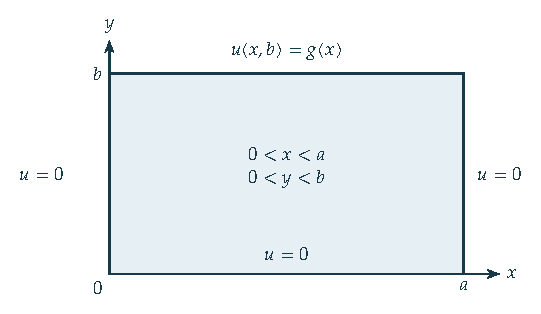
\includegraphics[width=10.25cm]{assets/M2-E0109-setup.pdf}\par
\smallskip{\small Dominio rectangular y datos prescritos en sus cuatro lados.\par}
\end{minipage}
\end{center}

\supportlinks{M2-E0109}{1}{0}
\exercise{M2-E0358}{Core · Intermedio}
Se comparan tres modelos idealizados en \(0<x<L\), con \(L>0\): difusión térmica \(u_t=\kappa u_{xx}\), vibración de una cuerda \(u_{tt}=c^2u_{xx}\) y equilibrio térmico sin fuentes \(U''=0\). El campo está normalizado y es adimensional; \(\kappa>0\) tiene unidades de longitud al cuadrado por tiempo y \(c>0\), de longitud por tiempo. En todos los casos, los valores en ambos extremos se mantienen en cero.

Un registro sintético, cuyo tipo de ensayo no está identificado, proporciona
\[
u(x,0)=\sin(\pi x/L),\qquad u_t(x,0)=0.
\]
Para este registro se exige que el campo y las derivadas que aparecen en cada modelo, además de \(u_t\), se prolonguen continuamente hasta \(t=0\). Determine qué modelos son compatibles con la información completa y explique qué papel desempeña la tasa inicial registrada en cada uno. Justifique la compatibilidad que afirme.

Otro registro, identificado como térmico, indica temperatura inicial normalizada \(u(x,0)=1\) para \(0<x<L\) y extremos a cero para todo \(t>0\). Se proponen dos clases de solución: una exige continuidad en el rectángulo cerrado \([0,L]\times[0,T]\), con \(T>0\); la otra exige una solución clásica para \(t>0\), continua hasta los extremos a cada tiempo positivo, y sólo el límite \(u(x,t)\to1\) para cada \(x\) interior fijo cuando \(t\downarrow0\). ¿Qué clase queda descartada por los datos de las esquinas? ¿Qué permite concluir esto sobre el modelo térmico para tiempos positivos?

\supportlinks{M2-E0358}{0}{0}
\exercise{M2-E0270}{Core · Intermedio}
Obtenga la solución formal de $u_t=u_{xx}$ para $0<x<\pi$, $t>0$, con $u_x(0,t)=u_x(\pi,t)=0$ y $u(x,0)=e^x$.

\supportlinks{M2-E0270}{0}{0}
\exercise{M2-E0356}{Core · Intermedio}
En un modelo adimensional de equilibrio térmico se cumple \(u_{xx}+u_{yy}=0\) en el cuadrado \(0<x<3\), \(0<y<3\). Se usa una malla de paso uno en ambas direcciones. Los valores de contorno son sintéticos; las cuatro incógnitas interiores aparecen en la tabla:
\[
\begin{array}{c|rrrr}
y\backslash x&0&1&2&3\\\hline
3&4&7&12&19\\
2&8&C&D&23\\
1&10&A&B&25\\
0&10&13&18&25
\end{array}
\]
Aproxime cada derivada segunda mediante la diferencia centrada correspondiente; por ejemplo,
\[
u_{xx}(i,j)\approx U_{i+1,j}-2U_{i,j}+U_{i-1,j}.
\]
Construya y resuelva el sistema para \(A,B,C,D\). Como referencia, examine el polinomio
\[
H(x,y)=x^2-y^2+2x+y+10.
\]
Compruebe su relación con la ecuación y los datos de la tabla, compare sus valores interiores con la solución del sistema y explique el alcance de ese acuerdo.

\Needspace{11.91cm}
\begin{center}
\begin{minipage}{\linewidth}
\centering
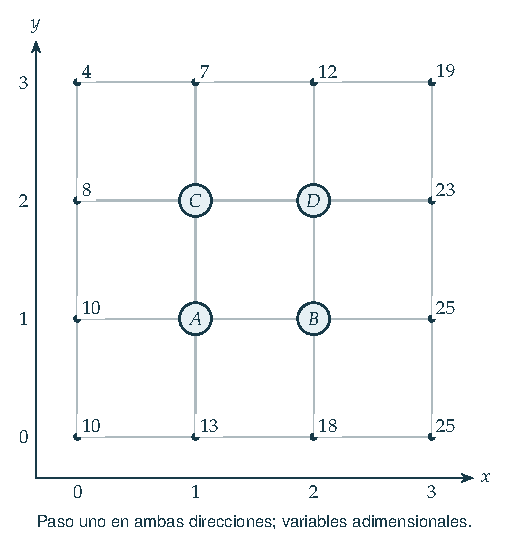
\includegraphics[width=9.66cm]{assets/M2-E0356-setup.pdf}\par
\smallskip{\small Posición de los datos de contorno y de las cuatro incógnitas interiores.\par}
\end{minipage}
\end{center}

\supportlinks{M2-E0356}{1}{0}
\exercise{M2-E0272}{Core · Intermedio}
Resuelva $u_t=\alpha^2u_{xx}$ para $0<x<L$, $t>0$, con $u(0,t)=0$, $u_x(L,t)=0$ y $u(x,0)=100$ en el interior. Suponga $L>0$ y $\alpha>0$.

\supportlinks{M2-E0272}{0}{0}
\exercise{M2-E0300}{Core · Intermedio}
Considere la ecuación de Laplace $u_{xx}+u_{yy}=0$ en el rectángulo
$0<x<a$, $0<y<b$, con $a,b>0$ y lados verticales aislados:
\[
u_x(0,y)=u_x(a,y)=0,\qquad 0<y<b.
\]
Resuelva los tres apartados en el orden indicado.

Los datos $f,g$ pertenecen a $C^2[0,a]$. Se busca una función continua
en el rectángulo cerrado, armónica en su interior y con derivadas hasta
orden dos continuas junto a los lados verticales para $0<y<b$.
Las condiciones Neumann se imponen en esos lados abiertos. No se impone
regularidad de las derivadas en los cuatro vértices; exigirla añadiría
compatibilidades a los datos.

\begin{enumerate}[label=(\alph*),ref=\alph*,leftmargin=*]
\item Obtenga por separación de variables la solución con $u(x,0)=f(x)$ y
$u(x,b)=0$. Incluya todos los modos espaciales admisibles.
\item Utilice el resultado del apartado anterior para resolver el problema con
$u(x,0)=f(x)$ y $u(x,b)=g(x)$.
\item Aplique el apartado anterior a $a=\pi$, $b=1$,
$f(x)=\cos x-\cos3x$ y $g(x)=\cos2x$.
\end{enumerate}

\supportlinks{M2-E0300}{0}{0}
\exercise{M2-E0268}{Core · Intermedio}
Una barra metálica de longitud $\pi\,\mathrm{cm}$ y difusividad térmica $1\,\mathrm{cm^2/s}$ tiene la superficie lateral aislada. Sus extremos se mantienen a $200\,{}^\circ\mathrm C$ en $x=0$ y $0\,{}^\circ\mathrm C$ en $x=\pi$. La temperatura inicial interior es $u(x,0)=0\,{}^\circ\mathrm C$. Determine $u(x,t)$ para $0<x<\pi$, $t>0$.

\supportlinks{M2-E0268}{1}{0}
\Needspace{12\baselineskip}
\section{Soluciones, datos y consistencia}
\exercise{M2-E0257}{Core · Básico}
Resuelva $u_{xx}+2u_x=2xy$.

\supportlinks{M2-E0257}{0}{0}
\exercise{M2-E0294}{Core · Básico}
Resuelva $u_x-4yu=3$, con $u(0,y)=5$, para valores reales de $x,y$.

\supportlinks{M2-E0294}{0}{0}
\exercise{M2-E0265}{Core · Intermedio}
Obtenga una solución formal de $u_t=2u_{xx}+4x$ para $0<x<\pi$, $t>0$, con $u(0,t)=u(\pi,t)=0$ y $u(x,0)=\sin x$.

\supportlinks{M2-E0265}{0}{0}
\exercise{M2-E0256}{Core · Básico}
Resuelva $u_{xy}+2yu_x=4xy$.

\supportlinks{M2-E0256}{0}{0}
\exercise{M2-E0275}{Core · Avanzado}
Resuelva $u_{tt}=\alpha^2u_{xx}+tx$ para $0<x<\pi$, $t>0$, con $\alpha>0$, $u(0,t)=u(\pi,t)=0$, $u(x,0)=\sin x$ y $u_t(x,0)=5\sin(2x)-3\sin(5x)$.

\supportlinks{M2-E0275}{0}{0}
\exercise{M2-E0261}{Core · Básico}
Resuelva $u_{xy}+2u_y=1$ para funciones de clase $C^2$ en un rectángulo abierto.

\supportlinks{M2-E0261}{0}{0}
\exercise{M2-E0106}{Core · Intermedio}
Una cuerda tensa de longitud L, fija en ambos extremos, se levanta hasta una altura h0>0
en el punto x=a, con0<a<L, formando dos segmentos rectos; después se suelta desde el reposo.
Sea c>0 la velocidad de propagación, constante. Trabajar en el modelo de pequeñas pendientes,
con h0/a y h0/(L\ensuremath{-}a) pequeños, sin amortiguamiento.

\begin{enumerate}[label=(\alph*),ref=\alph*,leftmargin=*]
\item Hallar la posición de la cuerda en función de x,t.
\item Determinar las frecuencias naturales y el armónico principal.
\end{enumerate}

\Needspace{5.1cm}
\begin{center}
\begin{minipage}{\linewidth}
\centering
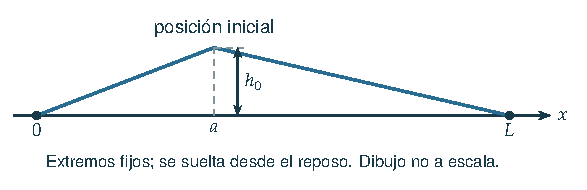
\includegraphics[width=11.13cm]{assets/M2-E0106-setup.pdf}\par
\smallskip{\small Forma inicial de la cuerda; el dibujo no está a escala.\par}
\end{minipage}
\end{center}

\supportlinks{M2-E0106}{0}{0}
\Needspace{12\baselineskip}
\section{Contrastes de perfiles y condiciones}
\exercise{M2-E0259}{Core · Básico}
Resuelva $u_{xx}+2u_x+u=xy$.

\supportlinks{M2-E0259}{0}{0}
\exercise{M2-E0274}{Core · Avanzado}
Una cuerda tensa de longitud $L>0$, con extremos fijos, parte de una posición recta $u(x,0)=0$. Su velocidad inicial es \[g(x)=u_t(x,0)=\begin{cases}V_0x/a,&0\le x\le a,\\ V_0(L-x)/(L-a),&a<x\le L,\end{cases}\] donde $0<a<L$. Usando $u_{tt}=\alpha^2u_{xx}$, con $\alpha>0$, determine la posición de la cuerda.

\supportlinks{M2-E0274}{0}{0}
\exercise{M2-E0267}{Core · Intermedio}
Un alambre de longitud $\pi\,\mathrm{cm}$ tiene difusividad térmica $1\,\mathrm{cm^2/s}$, superficie lateral aislada y extremos mantenidos a $0\,{}^\circ\mathrm C$. Inicialmente su temperatura interior es $25\,{}^\circ\mathrm C$. Una corriente eléctrica produce calor a razón de $5\,{}^\circ\mathrm C/\mathrm s$ en cada punto. Formule el modelo y determine $u(x,t)$ para $0<x<\pi$ y $t>0$.

Se usa conducción unidimensional homogénea, con difusividad constante y sin pérdidas laterales. La condición inicial uniforme corresponde al interior; las temperaturas de los extremos se imponen para $t>0$.

\supportlinks{M2-E0267}{0}{0}
\exercise{M2-E0253}{Core · Intermedio}
Resuelva $xu_x+u=4ye^{2x}$. Distinga las regiones con $x\ne0$ de las soluciones que se prolongan por $x=0$.

En cada región se buscan soluciones C1. Una prolongación por x=0 se entiende en un rectángulo que contiene esa recta y el intervalo de y considerado.

\supportlinks{M2-E0253}{0}{0}
\exercise{M2-E0299}{Core · Intermedio}
Una cuerda de longitud $L$ está fijada en sus extremos y obedece
\[
u_{tt}=\alpha^2u_{xx}-ku,\qquad 0<x<L,\quad t>0,
\qquad u(0,t)=u(L,t)=0,
\]
donde $L,\alpha,k>0$. Obtenga por separación de variables el desarrollo modal
del desplazamiento en los dos casos siguientes.

El dato de desplazamiento $f$ pertenece a $C^2[0,L]$ y el de velocidad
$g$ a $C^1[0,L]$, con $f(0)=f(L)=g(0)=g(L)=0$.
Se pide la solución modal de energía finita: los datos se recuperan en el
sentido cuadrático y las ecuaciones de cada modo se satisfacen exactamente.
No se presupone que la suma tenga dos derivadas continuas en todos los puntos
de la frontera. Cuando se justifique la diferenciación término a término,
la misma fórmula da la solución clásica.

\begin{enumerate}[label=(\alph*),ref=\alph*,leftmargin=*]
\item La cuerda parte del reposo con desplazamiento inicial $f(x)$:
$u(x,0)=f(x)$ y $u_t(x,0)=0$.
\item La cuerda parte de la posición recta con velocidad inicial $g(x)$:
$u(x,0)=0$ y $u_t(x,0)=g(x)$.
\end{enumerate}

\supportlinks{M2-E0299}{0}{0}
\exercise{M2-E0255}{Core · Intermedio}
Resuelva $u_{yy}+\sin(xy)=0$ para funciones de clase $C^2$.

\supportlinks{M2-E0255}{0}{0}
\exercise{M2-E0263}{Core · Básico}
Resuelva $u_t=3u_{xt}$, con $u(0,t)=e^{-t}$ y $u(x,0)=1$.

Se buscan soluciones $C^2$ en un rectángulo de $(x,t)$ que contenga los segmentos $x=0$ y $t=0$ usados en los datos.

\supportlinks{M2-E0263}{0}{0}
\Needspace{12\baselineskip}
\section{Precisión y límites del modelo}
\exercise{M2-E0269}{Core · Intermedio}
Obtenga la solución formal de $u_t=5u_{xx}$ para $0<x<1$, $t>0$, con $u(0,t)=u(1,t)=0$ y $u(x,0)=(1-x)x^2$.

\supportlinks{M2-E0269}{0}{0}
\exercise{M2-E0379}{Core · Intermedio}
En una barra con extremos a temperatura de referencia, \(U_j^n\) representa el exceso de temperatura, en kelvin. Hay sólo dos nodos interiores, separados por \(\Delta x=1\,\mathrm{cm}\), con \(U_0^n=U_3^n=0\). Para \(\kappa=1\,\mathrm{cm^2/s}\) se usa
\[
U_j^{n+1}=(1-2r)U_j^n+r(U_{j-1}^n+U_{j+1}^n),\qquad
r=\frac{\kappa\Delta t}{(\Delta x)^2}.
\]
Desde \((U_1^0,U_2^0)=(10,0)\), calcule un paso con \(\Delta t=0.6\,\mathrm{s}\). Halle el mayor paso que garantice temperaturas no negativas para \emph{cualquier} par inicial no negativo en esta malla.

Para el paso propuesto de \(0.6\,\mathrm{s}\), estudie también cómo se multiplican las perturbaciones proporcionales a \((1,1)\) y a \((1,-1)\). Decida si toda perturbación inicial decae al repetir pasos en esta malla fija. Explique por qué esa conclusión y la conservación de temperaturas no negativas son garantías distintas, y si alguna establece por sí sola la precisión del cálculo.

\supportlinks{M2-E0379}{0}{0}
\exercise{M2-E0266}{Core · Avanzado}
Una barra de cobre de longitud $100\,\mathrm{cm}$ tiene difusividad térmica $1.14\,\mathrm{cm^2/s}$. Sus extremos se mantienen inicialmente a $0\,{}^\circ\mathrm C$ y se aplica calor en el centro, $x=50\,\mathrm{cm}$, manteniéndolo a $100\,{}^\circ\mathrm C$ hasta alcanzar el estado estacionario. Use el modelo unidimensional de conducción con superficie lateral aislada.

El coeficiente $1.14$ es constante. Antes de $t=0$ la fuente central divide la barra en dos tramos estacionarios sin producción interior distribuida. Después se retira la fuente y se mantiene el modelo sin pérdidas laterales. La condición inicial posterior se impone en $0<x<100$; el cambio instantáneo del extremo izquierdo no permite continuidad conjunta en $(0,0)$.

\begin{enumerate}[label=(\alph*),ref=\alph*,leftmargin=*]
\item Determine la distribución estacionaria de temperatura mientras actúa la fuente central.
\item En $t=0$ se retira la fuente central y se eleva instantáneamente el extremo izquierdo a $20\,{}^\circ\mathrm C$, manteniendo el derecho a $0\,{}^\circ\mathrm C$. Determine $u(x,t)$ para $0<x<100$ y $t>0$.
\end{enumerate}

\Needspace{8.2cm}
\begin{center}
\begin{minipage}{\linewidth}
\centering
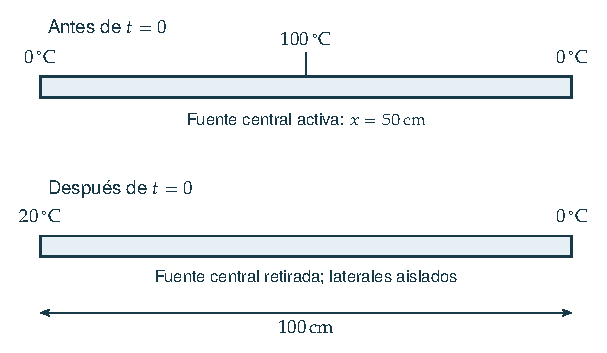
\includegraphics[width=11.52cm]{assets/M2-E0266-setup.pdf}\par
\smallskip{\small Condiciones impuestas antes y después de retirar la fuente central.\par}
\end{minipage}
\end{center}

\supportlinks{M2-E0266}{0}{0}
\exercise{M2-E0271}{Core · Intermedio}
Obtenga la solución formal de $u_t=3u_{xx}$ para $0<x<\pi$, $t>0$, con $u(0,t)=u(\pi,t)=100$ y $u(x,0)=400(x/\pi-1/2)^2$.

\supportlinks{M2-E0271}{0}{0}
\exercise{M2-E0380}{Core · Intermedio}
Se comprueba un cálculo idealizado de enfriamiento de una tira de longitud \(L=2\,\mathrm{cm}\), difusividad \(\kappa=1\,\mathrm{cm^2/s}\) y exceso de temperatura nulo en sus extremos. El perfil inicial es \(u(x,0)=10\sin(\pi x/L)\,\mathrm K\); la solución de referencia es
\[
u(x,t)=10e^{-\kappa\pi^2t/L^2}\sin(\pi x/L)\,\mathrm K.
\]
Se exige un error numérico en el centro no mayor que \(0.10\,\mathrm K\) en \(T=0.50\,\mathrm s\). Use el esquema explícito
\[
U_j^{n+1}=(1-2r)U_j^n+r(U_{j-1}^n+U_{j+1}^n),\qquad r=\kappa\Delta t/(\Delta x)^2.
\]
Primero tome \(\Delta x=1\,\mathrm{cm}\), \(\Delta t=0.25\,\mathrm s\), y avance el único nodo interior hasta \(T\). Después reduzca \(\Delta x\) a la mitad: decida si conservar el paso temporal garantiza estabilidad frente a perturbaciones y elija un nuevo paso que conserve \(r\).

Puede usar la condición suficiente \(0\le r\le1/2\) y que un modo discreto \(\sin(m\pi x/L)\) se multiplica por
\[
g_m=1-4r\sin^2\!\left(\frac{m\pi\Delta x}{2L}\right).
\]
En la malla fina, \(m=1,2,3\). Calcule la temperatura central refinada mediante una potencia de \(g_1\), sin hacer todos los pasos a mano. Compare ambos errores con la tolerancia. Explique por qué un paso estable no asegura precisión y por qué examinar sólo el perfil inicial puede ocultar una perturbación que crece. Se permite calculadora.

\supportlinks{M2-E0380}{1}{0}
\exercise{M2-E0058}{Core · Intermedio}
Una cuerda infinita que vibra libremente tiene velocidad inicial \(g(x)=xe^{-x^2}\).
En el modelo \(u_{tt}=c^2u_{xx}\), con rapidez constante \(c>0\), determinar la posición
inicial para que el movimiento sea una onda que viaje solo hacia el sentido positivo de x.

\supportlinks{M2-E0058}{0}{0}
\exercise{M2-E0357}{Core · Avanzado}
Una barra idealizada tiene longitud \(L>0\), difusividad constante \(\kappa>0\) y extremos mantenidos a la temperatura de referencia. Para la temperatura en exceso,
\[
u_t=\kappa u_{xx},\qquad 0<x<L,\quad t>0,
\qquad u(0,t)=u(L,t)=0,
\]
\[
u(x,0)=\Theta\left[3\sin\left(\frac{\pi x}{L}\right)
-\sin\left(\frac{2\pi x}{L}\right)\right],\qquad \Theta>0.
\]
La difusividad tiene unidades de longitud al cuadrado por unidad de tiempo y \(\Theta\) tiene unidades de temperatura.

Aplique la transformada de Laplace respecto de \(t\) a la PDE y a sus datos. Obtenga y resuelva el problema de contorno espacial para
\[
U(x,s)=\int_0^{\infty}e^{-st}u(x,t)\,dt,\qquad s>0,
\]
justifique su unicidad para cada \(s>0\) e invierta la transformada. Puede suponer inicialmente que las operaciones de transformación y las dos derivadas espaciales son intercambiables. Verifique en la función recuperada la ecuación, los datos y la existencia de las transformadas utilizadas.

\supportlinks{M2-E0357}{1}{0}
\appendix
\chapter{Pistas para desbloquear el trabajo}
Antes de consultar una pista, anota qué sabes y dónde te has detenido.
\supportheading{hint}{M2-E0183}
Antes de buscar una fórmula, comprueba qué exige la ecuación en el propio punto del dato inicial.

\supportheading{hint}{M2-E0368}
Distingue la cantidad de trabajo pendiente, el caudal real de salida y la capacidad nominal. Revisa cuáles están dados y cuáles dependen de una hipótesis tuya.

\supportheading{hint}{M2-E0363}
Revisa respecto de qué incógnita es lineal cada expresión. Si divides por una cantidad que puede anularse, guarda ese caso para comprobarlo en la ecuación original.

\supportheading{hint}{M2-E0310}
Escribe por separado el tiempo y el estado de cada evaluación antes de calcular la pendiente. Recuerda que una pendiente y el incremento que produce durante un paso son cantidades distintas.

\supportheading{hint}{M2-E0365}
Asocia cada dato inicial con la cantidad a la que se refiere. Si introduces una incógnita auxiliar, anota qué dato la determina y cuál necesitarás para recuperar la función original.

\supportheading{hint}{M2-E0076}
Compara los puntos problemáticos de la fórmula auxiliar con los coeficientes de la ecuación original. La validez de una integral en un intervalo y la posible prolongación de una solución son preguntas distintas.

\supportheading{hint}{M2-E0036}
Fija primero el sentido positivo y el signo de cada fuerza. Una vez escrito el modelo, relaciona las raíces de su ecuación característica con la forma de la respuesta.

\supportheading{hint}{M2-E0347}
Compara las contribuciones al cuadrado de la norma del error. El tamaño de un coeficiente por sí solo no tiene en cuenta la norma de la función que multiplica.

\supportheading{hint}{M2-E0316}
Sustituye primero el valor nulo del parámetro en la ecuación y utiliza una condición de derivada antes de ocuparte de la normalización.

\chapter{Respuestas de comprobación}
Compara el resultado después de tu intento. En los problemas abiertos, comprueba las condiciones y la coherencia del modelo; puede haber varias respuestas válidas.
\Needspace{12\baselineskip}
\section*{Capítulo 1}
\addcontentsline{toc}{section}{Capítulo 1}
\supportheading{answer}{M2-E0177}
$y(t)=1000e^{0.03t}$, para $t\ge0$ en la interpretación de la cuenta.

\supportheading{answer}{M2-E0143}
$m=1$ o $m=-1$.

\supportheading{answer}{M2-E0183}
No existe tal solución clásica.

\supportheading{answer}{M2-E0099}
Sí, en cada intervalo que no contenga un cero de $\cos x$; $C=0$ incluye la solución nula.

\supportheading{answer}{M2-E0140}
\noindent\textbf{(a)} EDO de orden $2$, grado $1$, lineal no homogénea.

\noindent\textbf{(b)} EDO de orden $1$, grado $2$ en la forma escrita; no lineal.

\noindent\textbf{(c)} EDO de orden $4$, grado $1$, lineal no homogénea.

\noindent\textbf{(d)} EDP de orden $2$ y grado $1$.

\noindent\textbf{(e)} EDO de orden $1$, grado $1$, no lineal; requiere $x\ne0$ e $y\ne-1/3$.

\noindent\textbf{(f)} EDO de orden $1$, grado $1$, no lineal en el dominio de líquido $y>0$.

\noindent\textbf{(g)} EDP de orden $2$ y grado $1$.

\supportheading{answer}{M2-E0098}
Sí: $y=(e^x-2)/(e^x-1)$, en $(-\infty,0)$ y $(0,\infty)$.

\supportheading{answer}{M2-E0100}
La familia contiene todas las soluciones no nulas, en intervalos que eviten $x=-C/3$. Falta $y=0$, válida en toda la recta.

\supportheading{answer}{M2-E0208}
$y=2+2\ln[(2+x^2)/3]$, $x\in\mathbb R$.

\supportheading{answer}{M2-E0179}
$y(t)=5e^{t^3/3}$, $t\in\mathbb R$.

\supportheading{answer}{M2-E0103}
$y=2(1+Ce^{4x})/(1-Ce^{4x})$ donde $1-Ce^{4x}\ne0$, junto con $y=-2$. El caso $C=0$ ya da $y=2$.

\supportheading{answer}{M2-E0024}
Unos $16692$ años antes de la medición de 1950, según el modelo y los datos suministrados.

\supportheading{answer}{M2-E0209}
$y=C\sec^2x$, $C\in\mathbb R$, en cada intervalo entre dos ceros consecutivos de $\cos x$.

\supportheading{answer}{M2-E0025}
\noindent\textbf{(a)} $T^{\prime}=-k(T-20)$ con $k>0$; $k$ se mide en $\mathrm{min}^{-1}$.

\noindent\textbf{(b)} $T(60)=22.8125\,{}^\circ\mathrm C$; el descenso desde el minuto 30 es $12.1875\,{}^\circ\mathrm C$.

\supportheading{answer}{M2-E0180}
$y\equiv0$ y las ramas de signo constante definidas por $y^2/2+\ln|y|=x^2/2+C$, $C\in\mathbb R$. Cada rama está definida en toda $\mathbb R$.

\supportheading{answer}{M2-E0194}
$y^3/3+y=x^3/3+x+4/3$, para todo $x\in\mathbb R$.

\supportheading{answer}{M2-E0027}
\noindent\textbf{(a)} $Q^{\prime}=0.4Q+50$, $Q(0)=50$.

\noindent\textbf{(b)} $Q(t)=175e^{0.4t}-125\,\mathrm g$; $Q(10)\approx9429.68\,\mathrm g$.

\supportheading{answer}{M2-E0192}
$y(x)=\exp(\int_0^x s/\cos s\,ds)$, $-\pi/2<x<\pi/2$.

\supportheading{answer}{M2-E0308}
La solución decrece y permanece estrictamente por encima de \(2\) para todo \(t\ge0\). No cruza ni alcanza ese equilibrio en tiempo finito; su límite es \(2\).

\supportheading{answer}{M2-E0372}
Las pendientes se anulan sobre \(y=t^2\), son positivas debajo y negativas encima. La solución que parte de cero queda debajo para \(t>0\) y crece. La que parte de dos baja hasta \((1,1)\), cruza allí la parábola con tangente horizontal y después crece. Las soluciones no se cruzan entre sí. La parábola de pendientes nulas no es una solución ni una barrera.

\supportheading{answer}{M2-E0319}
Las soluciones son
\[
y_+(t)=1+e^{-t^2/2},\qquad
 y_-(t)=1-e^{-t^2/2}.
\]
Ambas son pares. \(y_+>1\) crece para \(t<0\) y decrece para \(t>0\); \(y_-<1\) decrece para \(t<0\) y crece para \(t>0\). En \(0\), la primera tiene máximo \(2\) y la segunda mínimo \(0\), con tangentes horizontales, pero ninguna es constante. Sus cuatro límites cuando \(t\to\pm\infty\) valen \(1\).

\supportheading{answer}{M2-E0246}
$t_{1/2}=15\ln2/[-\ln(0.99957)]\simeq24174.35$ años.

\supportheading{answer}{M2-E0320}
El polinomio de menor grado es
\[
f(y)=y(y-1)^2,\qquad\text{y por tanto}\qquad y'=y(y-1)^2.
\]
En \(0\), las trayectorias se alejan por ambos lados. En \(1\), se acercan desde la izquierda y se alejan hacia la derecha. Si \(0<y(0)<1\), la solución crece, permanece en \((0,1)\) y tiende a \(1\) cuando \(t\to\infty\).

\supportheading{answer}{M2-E0318}
El modelo es \(m'=u-12m/(6+m)\), \(m(0)=4\), con kilogramos y minutos como unidades. Los caudales admisibles son
\[
0\le u\le\frac{36}{5}=7.2\quad\mathrm{kg/min}.
\]
Para \(u=7.2\,\mathrm{kg/min}\), la cantidad crece desde \(4\,\mathrm{kg}\) y se aproxima a \(9\,\mathrm{kg}\) sin alcanzarlos en tiempo finito. Si \(u>7.2\,\mathrm{kg/min}\), supera \(9\,\mathrm{kg}\) en un tiempo finito.

\supportheading{answer}{M2-E0248}
No llega a $70\,{}^\circ\mathrm F$ en tiempo finito. Llega a $70.1\,{}^\circ\mathrm F$ en $3\ln(2300)/\ln(23/13)$ minutos.

\supportheading{answer}{M2-E0032}
$h(t)=24-\dfrac4{15}t$ cm para $0\le t<90$ días; el vaciado se alcanza en $t=90$ días.

\supportheading{answer}{M2-E0101}
$(y^{\prime})^2-4xy^{\prime}+4y=0$.

\supportheading{answer}{M2-E0114}
$t_*=38400\,\mathrm s=10$ horas $40$ minutos.

\supportheading{answer}{M2-E0147}
\[(x^2-y^2)y^{\prime}=2xy.\] Donde $x^2\ne y^2$, equivale a $y^{\prime}=2xy/(x^2-y^2)$. La recta $y=0$ es una solución adicional de la EDO eliminada, no una circunferencia no degenerada.

\supportheading{answer}{M2-E0112}
$t=\dfrac{4.5\times10^9}{\ln2}\ln\!\left(1+\dfrac{14\cdot238}{100\cdot206}\right)\approx9.73335\times10^8$ años.

\supportheading{answer}{M2-E0146}
\[(x+y)^2\bigl(1+(y^{\prime})^2\bigr)=(1-y^{\prime})^2.\] Los centros de la familia pedida son $(a,-a)$ con $a<0$, en el segundo cuadrante. La ecuación diferencial por sí sola no impone esta restricción ni excluye sus soluciones envolventes.

\supportheading{answer}{M2-E0113}
\noindent\textbf{(a)} $k=\ln(11/2)/300\approx0.00568249$ por unidad de cantidad y por minuto.

\noindent\textbf{(b)} Si $R(t)=(11/2)^{t/30}$, $C(t)=20[R(t)-1]/[2R(t)-1]$, para $t\ge0$. Crece de $0$ a $10$ asintóticamente.

\supportheading{answer}{M2-E0321}
Con \(t\) en segundos,
\[
\omega(t)=3e^{-t/4}\quad\mathrm{rad/s},\qquad
\theta(t)=12(1-e^{-t/4})\quad\mathrm{rad}.
\]
Alcanza la marca de \(8\) rad en \(4\ln3\) segundos; no alcanza las de \(12\) ni \(15\) rad. Una marca \(\Theta>0\) se alcanza en tiempo finito exactamente cuando \(\Theta<12\) rad, en
\[
t_\Theta=4\ln\!\left(\frac{12}{12-\Theta}\right)\ \mathrm s,
\]
cuando \(\Theta\) se expresa numéricamente en radianes. \(\theta\to12\) rad y \(\omega\to0\), pero la velocidad angular no se anula en ningún tiempo finito.

\supportheading{answer}{M2-E0141}
\begin{enumerate}
\item Sí, en $\mathbb{R}$.
\item No es solución en ningún intervalo abierto no vacío: la igualdad sólo se cumple en $x=0$.
\item No en $\mathbb{R}$; sí en $(-\infty,0)$ y $(0,\infty)$. No es derivable en $0$.
\item Sí: define una única función derivable en $\mathbb{R}$, con $y'=(1+\cos x)/(1+3y^2)$.
\item La curva completa no es una gráfica. Cada rama $y=\pm\sqrt{\ln(1+x)}$ es solución en $(0,\infty)$; el punto $(0,0)$ no puede pertenecer a una solución de la EDO.
\item Sí, como función de $x$ en $\mathbb{R}$: $y'=2t/(1+3t^2)$.
\item Sí, en $\mathbb{R}$: la gráfica es $y=x^2+x$. En $t=0$ el cociente paramétrico es indeterminado, pero $y'(0)=1$.
\end{enumerate}

\supportheading{answer}{M2-E0211}
$I'=0.005I(101-I)$, $I(0)=1$; $I(t)=101/[1+100e^{-0.505t}]$. Los tiempos son $\ln100/0.505\simeq9.12$ y $\ln900/0.505\simeq13.47$, respectivamente.

\supportheading{answer}{M2-E0182}
$y\equiv-1$ y $y=K(x-1)/[x-K(x-1)]$, $K\in\mathbb R$, en intervalos que eviten $0$, $1$ y los ceros del denominador. El caso $K=0$ es $y\equiv0$.

\supportheading{answer}{M2-E0144}
\noindent\textbf{(a)} $(x^2-y)y'=xy$. Donde $x^2-y\ne0$, $y'=xy/(x^2-y)$.

\noindent\textbf{(b)} $xy''+y'=0$, con $x>0$.

\noindent\textbf{(c)} $y'''-2y''+y'=0$.

\noindent\textbf{(d)} $xy''-y'\ln y'=0$, con $y'>0$.

\supportheading{answer}{M2-E0191}
Además de $y\equiv0$, para cada $a\ge0$ y $\sigma\in\{-1,1\}$:
\[y(x)=\begin{cases}0,&x\le a,\\ \sigma[\tfrac23(x-a)]^{3/2},&x>a.\end{cases}\]

\supportheading{answer}{M2-E0130}
\noindent\textbf{(a)} $v(t)=\sqrt{mg/k}\,\tanh\!\bigl(\sqrt{gk/m}\,t\bigr)$.

\noindent\textbf{(b)} $t_*=\sqrt{m/(gk)}\,\operatorname{arcosh}\!\left(e^{kH/m}\right)$.

\supportheading{answer}{M2-E0193}
$y(x)=\tan(2-x-1/x)$ para $\alpha<x<\beta$, donde
\[A=2+\pi/2,\qquad \alpha=(A-\sqrt{A^2-4})/2,\quad\beta=(A+\sqrt{A^2-4})/2.\]

\supportheading{answer}{M2-E0142}
\begin{enumerate}
\item La EDO se verifica donde la tangente está definida, pero no en $\mathbb{R}$. Los intervalos máximos son $(-\pi/2+k\pi-C,\,\pi/2+k\pi-C)$, $k\in\mathbb{Z}$.
\item Los miembros son soluciones, pero sólo admiten $a\geq0$. Para $a>0$ hay dos valores $C=\pm\sqrt{a/2}$; para $a=0$, sólo $C=0$. La familia completa sin redundancia es $y_A=A(2+\sin x)$, $A\in\mathbb{R}$, con $A=a/2$.
\item El dominio es $\mathbb{R}$ si $C\geq0$ y $(\ln(-C),\infty)$ si $C<0$. Sólo $C=1$ produce una solución de la EDO indicada.
\item Todos los miembros son soluciones en $\mathbb{R}$, pero también lo es $z(x)=xe^{-x^2}$. Esta función no pertenece a la familia en ningún intervalo abierto no vacío, pues $z(x)/e^{-x^2}=x$ no es constante.
\item La parametrización dada recorre sólo $(0,\infty)$ y verifica la EDO. Para $x<0$ sirve $x=-e^t$, $y=C+e^{-t}$, $t\in\mathbb{R}$. En ambos casos la gráfica es $y=C-1/x$ en la componente correspondiente.
\end{enumerate}

\supportheading{answer}{M2-E0195}
Para $-\infty\le a\le0\le b\le\infty$:
\[y(x)=\begin{cases}-(x-a)^2,&x<a\quad(a> -\infty),\\0,&a\le x\le b,\\(x-b)^2,&x>b\quad(b<\infty).\end{cases}\]
Un extremo infinito significa que falta la rama correspondiente. En particular, no hay unicidad.

\supportheading{answer}{M2-E0145}
\[(x^2+y^2)y^{\prime\prime}+2(y-xy^{\prime})\bigl(1+(y^{\prime})^2\bigr)=0.\] La ecuación eliminada también admite rectas por el origen; estas no pertenecen a la familia de circunferencias no degeneradas.

\supportheading{answer}{M2-E0102}
Donde $y\ne-1$, $y=[x^2/6-x+C]^3-1$. También $y=-1$ y los empalmes $C^1$ de estas ramas con tramos $y=-1$, en ceros del corchete.

\supportheading{answer}{M2-E0368}
La capacidad nominal por sí sola no determina el vaciado. Un servicio a plena capacidad mientras haya trabajo vacía el estado continuo en \(3\) min y lo mantiene en cero. Otro modelo, con salida \(\min(q/\tau,10)\) y \(\tau=1\) min, conserva trabajo pendiente y tiende a \(6\) piezas. La conclusión debe acompañarse de la ley elegida y su interpretación.

\Needspace{12\baselineskip}
\section*{Capítulo 2}
\addcontentsline{toc}{section}{Capítulo 2}
\supportheading{answer}{M2-E0196}
$y(x)=\tfrac13e^{-x}+e^{-4x}$, $x\in\mathbb R$.

\supportheading{answer}{M2-E0026}
$p(t)=0.05+0.15e^{-t/10}$, expresado en porcentaje; $p(20)\approx0.0703003\%$.

\supportheading{answer}{M2-E0197}
$y=e^{-x^2}(e^x-2)$ en $\mathbb R$.

\supportheading{answer}{M2-E0156}
\noindent\textbf{(a)} $y=\sin x+C\cos x$.

\noindent\textbf{(b)} La misma familia $y=\sin x+C\cos x$.

\supportheading{answer}{M2-E0028}
\noindent\textbf{(a)} $m\gamma T^{\prime}=q-K(T-T_a)$; $T(t)=T_a+\dfrac qK(1-e^{-Kt/(m\gamma)})$.

\noindent\textbf{(b)} $T_r=T_a+q/K$. Solo se alcanza en el límite $t\to\infty$; para todo tiempo finito $T<T_r$.

\supportheading{answer}{M2-E0167}
$\mu(x)=\cos x$ y $y=(C-\sin x)/\cos x$, sobre cada intervalo donde $\cos x\ne0$.

\supportheading{answer}{M2-E0247}
Si $k\ne0$, $P=(P_0+r/k)e^{kt}-r/k$; si $k=0$, $P=P_0+rt$. Para $k<0$, $P\to-r/k>0$; para $k\ge0$, $P\to\infty$. No hay extinción futura con $r>0$.

\supportheading{answer}{M2-E0020}
$y=\dfrac{-x^2-1}{x-1}$ para $-\infty<x<1$.

\supportheading{answer}{M2-E0187}
\noindent\textbf{(a)} $y=e^{-x}(C+\arctan e^x)$, $x\in\mathbb R$.

\noindent\textbf{(b)} $y=e^{-x}(C+x^2)+x^2-2x+2$, $x\in\mathbb R$.

\noindent\textbf{(c)} $y=(C-x\cos x+\sin x)/(x\sin x)$, en cada intervalo $(n\pi,(n+1)\pi)$, $n\in\mathbb Z$.

\supportheading{answer}{M2-E0220}
$(x^2-1)y=C$. En intervalos que evitan $x=\pm1$, $y=C/(x^2-1)$. La solución nula puede atravesar ambos puntos.

\supportheading{answer}{M2-E0018}
\noindent\textbf{(a)} Primer orden y grado uno; exacta. Para $x\ne0$, lineal no homogénea y homogénea en el sentido $y^{\prime}=F(y/x)$.

\noindent\textbf{(b)} $xy-x^2/2=C$. Para $x\ne0$, $y=x/2+C/x$. La única solución clásica que atraviesa $0$ es $y=x/2$.

\supportheading{answer}{M2-E0221}
$xe^{2y}-\sin(xy)+y^2=C$. Define un gráfico suave allí donde $2xe^{2y}-x\cos(xy)+2y\ne0$.

\supportheading{answer}{M2-E0205}
\noindent\textbf{(a)} $-f(x)\,dx+[1/g(y)]\,dy=0$ es exacta donde $g\ne0$. Las soluciones constantes $y=y_*$ con $g(y_*)=0$ se comprueban en la ecuación original.

\noindent\textbf{(b)} $-x\,dx+dy/y=0$ para $y\ne0$, con potencial $-x^2/2+\log|y|$. La familia completa es $y=Ce^{x^2/2}$, $C\in\mathbb R$.

\supportheading{answer}{M2-E0021}
$y=0$ y las ramas de $xy+\ln|y|=C$ con $y\ne0$ y $xy+1\ne0$.

\supportheading{answer}{M2-E0204}
\noindent\textbf{(a)} $\mu=y$, con $y\ne0$; la forma resultante es $dx+3y^2\,dy$.

\noindent\textbf{(b)} $\mu=e^x$; la forma resultante es $e^x\,dx-e^{-y}\,dy$.

\noindent\textbf{(c)} $\mu=y^2$, $y\ne0$; queda $(\cos x+y)\,dx+x\,dy$.

\noindent\textbf{(d)} $\mu=x$, $x\ne0$; queda $(2xy+y^2)\,dx+(2xy+x^2)\,dy$.

\supportheading{answer}{M2-E0234}
En $y\ne0$ sirve $\mu=y^3$ y la integral es $y^4(x^2+y^2-10)=C$. Se añade el gráfico $y\equiv0$.

\supportheading{answer}{M2-E0131}
\noindent\textbf{(a)} $y=-\sqrt{[-x^3+\sqrt{x^6+8}]/2}$, para todo $x\in\mathbb R$.

\noindent\textbf{(b)} La raíz positiva de $(x+1)y+x^2y^3=1$, para todo $x\in\mathbb R$.

\supportheading{answer}{M2-E0250}
$x^2y^2+x^3=C$. Los gráficos regulares son $y=\pm\sqrt{C/x^2-x}$ donde $x\ne0$ y el radicando es positivo. No hay gráfico clásico que atraviese $x=0$ o $y=0$.

\supportheading{answer}{M2-E0133}
Para $x+y^2\ne0$, $(x-y^2)/(x+y^2)^2=C$. También $x+y^2=0$, cuyas ramas gráficas son $y=\pm\sqrt{-x}$ en $x<0$.

\supportheading{answer}{M2-E0019}
\noindent\textbf{(a)} $y=x-\dfrac{Ce^{2x}-1}{Ce^{2x}+1}$, donde el denominador no se anula, y $y=x-1$; la familia incluye $y=x+1$ con $C=0$.

\noindent\textbf{(b)} $y=x(\ln|x|+C)$ en intervalos contenidos en $x>0$ o $x<0$.

\noindent\textbf{(c)} $y=-\ln(1+Ce^x)$ sobre cualquier componente de $1+Ce^x>0$.

\supportheading{answer}{M2-E0104}
$x+y+2=Ce^y$, con $x+y+1\ne0$. El caso $C=0$ da $y=-x-2$.

\supportheading{answer}{M2-E0207}
$y\equiv0$ y $y=\pm[x/2-1/20+Ce^{-10x}]^{-1/2}$ en cada intervalo donde el corchete sea positivo.

\supportheading{answer}{M2-E0185}
\noindent\textbf{(a)} $y^3=1+C/x^3$ para $x\ne0$, conservando sólo intervalos donde el segundo miembro no se anula. La rama $y=1$ se prolonga a todo $\mathbb R$. No existe la solución $y=0$.

\noindent\textbf{(b)} $y=0$ o $y=[Ce^{3x}+x+1/3]^{-1/3}$, usando la raíz cúbica real en intervalos donde el denominador no se anula.

\supportheading{answer}{M2-E0111}
$x+y+1=C\exp((2x+y)/3)$, con $x+y\ne2$. El caso $C=0$ da $y=-x-1$.

\supportheading{answer}{M2-E0105}
Si $a\ne0$, con $b=|a|$, $y-b\arctan((x+y)/b)=C$, sobre ramas con $x+y\ne0$. Si $a=0$, las soluciones $C^1$ en un intervalo son $y=C$ o $y=-x$.

\supportheading{answer}{M2-E0164}
$y^3-3x^2y=1$: para cada $x\in\mathbb R$ se toma su única raíz positiva que cumple $y>\sqrt3|x|$ cuando $x\ne0$. La solución es global, positiva y par.

\supportheading{answer}{M2-E0149}
\noindent\textbf{(a)} $x^3(x+y)^2(x-2y)=C$. Para $C=0$ los arcos gráficos son $y=-x$ o $y=x/2$; ambos satisfacen la ecuación incluso en el origen.

\noindent\textbf{(b)} $3x+6y-\log|6x+3y+5|=C$, y además $y=-2x-5/3$. Se excluye $2x+y=-3/2$.

\supportheading{answer}{M2-E0210}
Defina $B(x)=e^{-4}+4\int_1^x e^{-4s}s^{-4}\,ds$. Entonces
\[y(x)=x^{-1}e^{-x}B(x)^{-1/4},\qquad\rho<x<\infty,\]
donde $\rho\in(0,1)$ es la única raíz de $B$.

\supportheading{answer}{M2-E0148}
\noindent\textbf{(a)} $y=0$, y los arcos de $(y-x)^3=Cxy$, con $x\ne0$ y $x+2y\ne0$. El caso $C=0$ contiene $y=x$.

\noindent\textbf{(b)} $y=\pm x$ y las ramas $y=(Cx^2+C^{-1})/2$, $C\ne0$, restringidas por $Cx^2-C^{-1}\ge0$. Pueden incluirse empalmes $C^1$ con $y=\pm x$ en los puntos de contacto admisibles; sin esta posibilidad, la lista de soluciones es incompleta.

\supportheading{answer}{M2-E0218}
$A_w h'=-c\pi(0.05)^2\sqrt{19.6h}$, para $0<h\le3$, con longitudes en metros y tiempo en segundos.

\supportheading{answer}{M2-E0232}
\noindent\textbf{(a)} $I(t)=1.2(1-e^{-20t})\,\mathrm A$, $t\ge0$, con $t$ en segundos.

\noindent\textbf{(b)} La fórmula integral satisface $LI^{\prime}+RI=E(t)$ e $I(0)=C$. Si $E(t)=E_0$, \[I(t)=\frac{E_0}{R}+\left(C-\frac{E_0}{R}\right)e^{-Rt/L},\qquad \lim_{t\to\infty}I(t)=\frac{E_0}{R}.\] El segundo sumando es el transitorio; el límite se afirma para tensión constante.

\supportheading{answer}{M2-E0219}
$\frac{25\pi}{144}h^2h'=-0.6\pi(0.02)^2\sqrt{19.6h}$, o $h'=-0.0013824\sqrt{19.6}\,h^{-3/2}$, para $0<h\le6$ en las unidades indicadas.

\supportheading{answer}{M2-E0022}
\noindent\textbf{(a)} $T(t)=Ce^{-kt}+\dfrac{kA_0}{k^2+\omega^2}[k\cos(\omega t)+\omega\sin(\omega t)]$.

\noindent\textbf{(b)} La diferencia entre dos soluciones es $(T_1(0)-T_2(0))e^{-kt}$ y tiende a cero. Queda el régimen periódico de la respuesta anterior.

\supportheading{answer}{M2-E0029}
\noindent\textbf{(a)} $S(t)=3(40-t)-\dfrac{3}{1600}(40-t)^3\,\mathrm{kg}$ para $0\le t<40$ minutos.

\noindent\textbf{(b)} $45\,\mathrm{kg}$, en $t=20$ minutos.

\noindent\textbf{(c)} $t_*=40(1-1/\sqrt3)\approx16.906$ minutos; $S_{\max}=80/\sqrt3\approx46.188$ kg.

\supportheading{answer}{M2-E0031}
$S(t)=\dfrac{25+t}{5}-\dfrac{125}{25+t}$ kg para $0\le t\le25$ min; $S(t)=10-\dfrac52e^{-(t-25)/25}$ kg para $t\ge25$ min.

\supportheading{answer}{M2-E0317}
Con \(t\) en minutos, el volumen es \(V(t)=50+2t\) litros. El dosificador debe aportar
\[
r(t)=1+0.10t\quad\mathrm{g/min}.
\]
La capacidad del depósito permite llegar hasta \(t=15\) min, mientras que la del dosificador permite seguir la concentración solicitada sólo hasta \(t=10\) min, inclusive. Limita primero el dosificador; entonces hay \(70\,\mathrm L\), a \(0.20\,\mathrm{g/L}\).

\supportheading{answer}{M2-E0138}
\noindent\textbf{(a)} Lineal no homogénea; la forma explícita requiere $x\ne0,-1$.

\noindent\textbf{(b)} Reducible a separable mediante $u=x-y+2$; si $a=0$, es $y^{\prime}=0$.

\noindent\textbf{(c)} Exacta.

\noindent\textbf{(d)} Lineal no homogénea y reducible a separable.

\noindent\textbf{(e)} Homogénea por cambio $y=ux$ en cada semieje x, con $xy\ge0$; la forma explícita exige además $y\ne0$.

\noindent\textbf{(f)} Separable; también Bernoulli de exponente -1 para y(x) donde $xy\ne0$.

\noindent\textbf{(g)} Exacta y reducible a separable mediante $u=x+3y$.

\noindent\textbf{(h)} Separable en su dominio $\cos y\ne0$.

\noindent\textbf{(i)} Homogénea, exacta en forma diferencial y Bernoulli de exponente -1 para $xy\ne0$.

\supportheading{answer}{M2-E0364}
Para \(\alpha\ne-1\),
\[
y(x)=C x^{-(\alpha+2)}-\frac{1}{(\alpha+1)x};
\]
para \(\alpha=-1\),
\[
y(x)=\frac{C-\log x}{x}.
\]
Todas estas expresiones están definidas en \(x>0\). La forma escrita es exacta cuando \(\alpha=0\); si \(\alpha=-2\), desaparece el término en \(y\) y basta una cuadratura directa.

\supportheading{answer}{M2-E0184}
\noindent\textbf{(a)} $y=(C/x+x/2)e^{-2x}$ para $x\ne0$. Sólo $C=0$ permite la prolongación por $x=0$, que da $y=(x/2)e^{-2x}$ en toda la recta.

\noindent\textbf{(b)} $y=(x+1)^2(1+x+x^2/2)$, con intervalo máximo $(-1,\infty)$.

\noindent\textbf{(c)} $y=2-(1+x^2)^{-3/2}$ en $\mathbb R$.

\noindent\textbf{(d)} $y=(x^3-3x+C)/[3x(x+1)]$ para $x\ne0,-1$. Si $C=0$, se prolonga por $x=0$ como $y=(x^2-3)/[3(x+1)]$, con $y(0)=-1$. Siempre se excluye $x=-1$.

\supportheading{answer}{M2-E0163}
$y=x+2+Ke^{-y}$, $K\in\mathbb R$, o equivalentemente $x=y-2-Ke^{-y}$. La segunda forma parametriza también los puntos donde la trayectoria tiene tangente vertical.

\supportheading{answer}{M2-E0363}
Sea \(A(t)=t+t^2/2\). Para la primera ecuación,
\[
y=e^{-A(t)}\left(C+\int_0^t s e^{A(s)}\,ds\right),\qquad t\in\mathbb R.
\]
Para la segunda, además de \(y\equiv0\),
\[
y=\frac{e^{-A(t)}}{C-\int_0^t s e^{-A(s)}\,ds},
\]
en cada intervalo conectado donde el denominador no se anule. Las constantes de las dos ecuaciones son independientes.

\supportheading{answer}{M2-E0190}
\noindent\textbf{(a)} $y=1+Ce^{-x^2/2}$, $x\in\mathbb R$.

\noindent\textbf{(b)} $y=e^x/7+Ce^{-6x}$, $x\in\mathbb R$.

\noindent\textbf{(c)} $y=(2-\cos x)e^{-x^3}$, $x\in\mathbb R$.

\noindent\textbf{(d)} $y=1+Ce^{-\sin x}$, $x\in\mathbb R$.

\noindent\textbf{(e)} \[y(x)=3e^{-x^4/4-x^2/2}\int_0^x(1+s^2)e^{s^4/4+s^2/2}\,ds,\qquad x\in\mathbb R.\]

\noindent\textbf{(f)} $y=1+2e^{1+\cos(2x)}$, $x\in\mathbb R$.

\supportheading{answer}{M2-E0175}
\noindent\textbf{(a)} $\mu_1=(y^2-x^2+1)^{-2}$ y $x/(y^2-x^2+1)=C$ donde el denominador no se anula. Se recupera separadamente $y^2=x^2-1$.

\noindent\textbf{(b)} $\mu_2=x^{-2}$ y $y^2=x^2+Kx-1$. Las soluciones gráficas reales son $y=\pm\sqrt{x^2+Kx-1}$ en intervalos de radicando estrictamente positivo.

\noindent\textbf{(c)} La familia completa es $y=\pm\sqrt{x^2+Kx-1}$, con radicando positivo. El caso $K=0$ es precisamente el que excluye el primer factor.

\supportheading{answer}{M2-E0249}
$y=C/[x\sqrt{|\cos x|}]$ en cada intervalo con $x\cos x\ne0$. La solución $y\equiv0$ también es válida y atraviesa los puntos degenerados.

\supportheading{answer}{M2-E0202}
\noindent\textbf{(a)} En $x>0$, la rama del dato es $y=x/(1-\log x)$, $0<x<e$. Se prolonga por $x=0$ con $y(0)=y^{\prime}(0)=0$; a la izquierda se puede unir $y=0$ o una rama $y=x/(A-\log|x|)$, evitando su polo. La prolongación hacia $x<0$ no es única.

\noindent\textbf{(b)} $y=\pm\sqrt{2Cx+C^2}$, $C>0$, en $x>-C/2$, junto con $y=0$ en intervalos de $x>0$. No hay solución gráfica $C^1$ en un intervalo abierto que atraviese el origen.

\noindent\textbf{(c)} $y=\sqrt{x^2/2+7/(2x^2)}$, $x\in(0,\infty)$.

\noindent\textbf{(d)} $y=(3-x^2)/(2x)$, $x\in(0,\infty)$.

\supportheading{answer}{M2-E0222}
$y(x)=\sqrt{[4-\sin^2x]/(1-x^2)}$, $-1<x<1$.

\supportheading{answer}{M2-E0135}
\noindent\textbf{(a)} $P_y-Q_x=nQ/x-mP/y$.

\noindent\textbf{(b)} $\mu=x^{-8}y^{-10}$; $1/(3x^6y^9)+1/(7x^7y^7)=C$ en las ramas regulares con $xy\ne0$. Además, $y=0$ es solución.

\supportheading{answer}{M2-E0132}
\noindent\textbf{(a)} No: $M_y=3x^2y^2$ y $N_x=1+y^2$.

\noindent\textbf{(b)} $\mu=1/(xy^3)$. Las soluciones no nulas verifican $x^2-y^{-2}+2\ln|y|=C$; además $y=0$.

\noindent\textbf{(c)} No, como función válida en una región abierta.

\supportheading{answer}{M2-E0199}
\noindent\textbf{(a)} El modelo de acción de masas es $A^{\prime}=B^{\prime}=-k_1AB$, $C^{\prime}=k_1AB-k_2C$, $D^{\prime}=k_2C$. Sus balances son $A-B=A_0-B_0$ y $B+C+D=B_0$. La aproximación sustituye $k_1AB$ por $\lambda B$.

\noindent\textbf{(b)} $B=B_0e^{-\lambda t}$, $A=A_0-B_0+B$, $D=B_0-B-C$, y\[C(t)=\begin{cases}\dfrac{\lambda B_0}{k_2-\lambda}(e^{-\lambda t}-e^{-k_2t}),&\lambda\ne k_2,\\ \lambda B_0t e^{-\lambda t},&\lambda=k_2.\end{cases}\]A primer orden relativo en $B_0/A_0$, se puede resumir $A\simeq A_0$.

\noindent\textbf{(c)} $C_{\max}=B_0/e$, alcanzado en $t_*=1/k_2$. La independencia se refiere al valor máximo del modelo de reactivo en exceso.

\supportheading{answer}{M2-E0309}
\[
100c'=-(q+100k)c,\qquad \frac q{100}+k=0.12.
\]
La primera curva admite \(0<q\le12\,\mathrm{L/min}\) y \(k=0.12-q/100\). El trazador identifica
\[
q=10\ln2\approx6.931\,\mathrm{L/min},\qquad
k=0.12-\frac{\ln2}{10}\approx0.05069\,\mathrm{min}^{-1}.
\]

\supportheading{answer}{M2-E0136}
\noindent\textbf{(a)} Si $s=x^2+y^2$ y $\theta$ es un ángulo local con $d\theta=(y\,dx-x\,dy)/s$, un potencial es $F=\theta+\tfrac12\int^s f(u)/u\,du$.

\noindent\textbf{(b)} $4\theta+(x^2+y^2)^2=C$ en la región elegida; por ejemplo, $4\arctan(x/y)+(x^2+y^2)^2=C$ donde esa rama sea válida.

\supportheading{answer}{M2-E0168}
\noindent\textbf{(a)} \[\alpha=\frac{4bc-3ab-ae}{ae-bc},\qquad \beta=\frac{bc+3ce-4ae}{ae-bc}.\]

\noindent\textbf{(b)} Para $y\ne0$, $\mu=y^{-2}$ y $\frac12x^4y^2+3x/y=C$, equivalentemente $\frac12x^4y^3+3x=Cy$. Se añade $y=0$.

\supportheading{answer}{M2-E0173}
\noindent\textbf{(a)} No: $M_y-N_x=-2/y^2-2x/(3y)+y/x^2$ no es idénticamente cero.

\noindent\textbf{(b)} Sí: $\mu=xy$. Una integral primera es $x^3y+3x^2+y^3=C$, con $xy\ne0$.

\noindent\textbf{(c)} No existe un factor de esa forma en una región abierta del dominio.

\supportheading{answer}{M2-E0172}
$\mu=1/[y\sqrt{x^2+y^2}]$ para $y\ne0$. Las ramas no nulas cumplen $x+\sqrt{x^2+y^2}=C>0$, o $y=\pm\sqrt{C^2-2Cx}$ en $x<C/2$. Se añade $y=0$.

\supportheading{answer}{M2-E0189}
\noindent\textbf{(a)} $(x^2-y^2-1)y^{\prime}=2xy$, o la forma implícita $-2xy\,dx+(x^2-y^2-1)\,dy=0$.

\noindent\textbf{(b)} $x^2+y^2+1=Cx$, $|C|>2$, junto con la recta $x=0$. Los valores $C=\pm2$ son puntos degenerados y no trayectorias regulares.

\supportheading{answer}{M2-E0200}
\noindent\textbf{(a)} \[A^{\prime}=-k_1AE+k_2B,\quad B^{\prime}=k_1AE-(k_2+k_3)B,\quad C^{\prime}=k_3B,\quad E^{\prime}=-k_1AE+(k_2+k_3)B.\]En el modelo reducido se sustituye $k_1AE$ por $\lambda E$.

\noindent\textbf{(b)} $E(t)=E_0-B(t)$.

\noindent\textbf{(c)} Con $K=\lambda+k_2+k_3$,\[B=\frac{\lambda E_0}{K}(1-e^{-Kt}),\qquad E=E_0-B,\]\[C=\frac{k_3\lambda E_0}{K}\left[t-\frac{1-e^{-Kt}}K\right],\qquad A=A_0-B-C.\]La aproximación requiere $(B+C)/A_0\ll1$; a ese orden $A\simeq A_0$.

\supportheading{answer}{M2-E0171}
$\alpha=-3$, $f(v)=1/[v(1+v^2)]$, de modo que $\mu=1/[y(x^2+y^2)]$. En $xy\ne0$, $x+\log|y|-\tfrac12\log(x^2+y^2)=C$, equivalentemente $\sqrt{x^2+y^2}=K|y|e^x$, $K>0$. Se añade $y=0$.

\supportheading{answer}{M2-E0174}
\noindent\textbf{(a)} $f(u)=u^{-3}$ y $\mu=y/x^3$, en $xy\ne0$.

\noindent\textbf{(b)} $2y^3-3y^2/x^2=C$ para $x\ne0$, junto con $y=0$. Las prolongaciones $C^1$ por el origen se comprueban mediante la ecuación original.

\supportheading{answer}{M2-E0139}
\noindent\textbf{(a)} No: $M_y=-\tan^2(xy)/x$ y $N_x=0$.

\noindent\textbf{(b)} No existe tal factor integrante en ninguna región abierta no vacía del dominio natural.

\noindent\textbf{(c)} $\mu=\cos(xy)$ y $\sin(xy)=Cx$. Sus ramas son $y=[n\pi+(-1)^n\arcsin(Cx)]/x$, $n\in\mathbb Z$, en intervalos con $x\ne0$ y $|Cx|<1$.

\supportheading{answer}{M2-E0373}
Duplicar \(C\) reduce a la mitad la pendiente inicial sin cambiar la tensión límite; duplicar \(G\) conserva la pendiente inicial y reduce a la mitad el límite. La respuesta original queda por encima de las dos modificadas para \(t>0\). Las dos modificadas se cruzan una vez: al principio es mayor la de conductancia doble; después lo es la de capacidad doble.

\supportheading{answer}{M2-E0030}
\noindent\textbf{(a)} $V=50+5t$, $S=10t$ para $0\le t\le3$; $V=68-t$, $S=2(68-t)-\dfrac{100}{65^6}(68-t)^6$ para $3\le t<68$. V se mide en litros y S en gramos.

\noindent\textbf{(b)} $c=\dfrac{2t}{10+t}$ g/L para $0\le t\le3$ y $c=2-\dfrac{100}{65^6}(68-t)^5$ g/L para $3\le t<68$. Cuando $t\to68^-$, $S\to0$ y $c\to2$ g/L; el modelo no define concentración ni evolución posterior en un tanque vacío.

\noindent\textbf{(c)} $V_*=65(13/60)^{1/5}\approx47.8709$ L; $t_*=68-V_*\approx20.1291$ min; $S_*=5V_*/3\approx79.7849$ g.

\supportheading{answer}{M2-E0023}
\noindent\textbf{(a)} Sea $u(x)=e^{5x^3/3-5x}\left[e^{10/3}+5\int_1^x s e^{-5s^3/3+5s}\,ds\right]$. Entonces $y=u^{-1/5}$ en la componente de $u>0$ que contiene $1$.

\noindent\textbf{(b)} $y(x)=e^{-x^2/2}\left[1-3\int_0^x e^{-3s^2/2}\,ds\right]^{-1/3}$ en $(-\infty,\beta)$, donde $\int_0^\beta e^{-3s^2/2}\,ds=1/3$.

\noindent\textbf{(c)} $y=2/(3x-2)$, con $x\in(2/3,\infty)$.

\supportheading{answer}{M2-E0307}
Si \(S(t)\) es la temperatura del sensor y \(e(t)=R(t)-S(t)\) es la diferencia entre proceso y lectura, \(3S'=R-S\) y \(e'=2-e/3\). Así,
\[
e(t)=6(1-e^{-t/3}),\qquad S(t)=14+2t+6e^{-t/3}.
\]
La lectura es admisible para \(0\le t\le3\ln3\approx3.296\,\mathrm s\). Para diez segundos,
\[
a_{\max}=\frac{4}{3(1-e^{-10/3})}\approx1.383\,{}^\circ\mathrm C/\mathrm s.
\]

\supportheading{answer}{M2-E0115}
\noindent\textbf{(a)} $t\approx207.072874\,\mathrm s$ desde el inicio de la caída.

\noindent\textbf{(b)} $t\approx87.122326\,\mathrm s$ desde el inicio; no $66$ s.

\supportheading{answer}{M2-E0166}
\noindent\textbf{(a)} $x^2\cos y+x^3y-y^2/2=C$.

\noindent\textbf{(b)} $x^3+3x^2y+3xy^2-3y=4$. Su rama inicial es\[y=\frac{3-3x^2+\sqrt{9-18x^2-3x^4+48x}}{6x},\quad 0<x<\alpha,\]donde $\alpha\in(1,2)$ es la única raíz positiva de $x^4+6x^2-16x-3=0$.

\noindent\textbf{(c)} $y^2\sin x-x^3y-x^2+y\log y-y=0$, en la rama regular que pasa por $(0,e)$ y permanece en $y>0$.

\noindent\textbf{(d)} $x^2/y^2+xy=C$ para $y\ne0$, y además $y=0$. Por el origen hay además prolongaciones $C^1$ de las ramas $C>0$, con pendiente $\pm1/\sqrt C$; la misma constante y el mismo signo de pendiente deben mantenerse a ambos lados.

\noindent\textbf{(e)} $x^2/y+xy+y^2=C$ para $y\ne0$, y además $y=0$. Por el origen, cada $C\ne0$ tiene una rama analítica con $y=x^2/C+O(x^5)$ y $y^{\prime}(0)=0$. Pueden empalmarse a cada lado esas ramas con constantes independientes o con la rama cero, conservando clase $C^1$. El nivel $C=0$ no aporta una rama no nula $C^1$ por el origen.

\supportheading{answer}{M2-E0206}
\noindent\textbf{(a)} $P'=0.15(1+t^2)P+20$, $P(0)=100$.

\noindent\textbf{(b)} $P'(0)=35$ personas por año.

\noindent\textbf{(c)} Si $t_*$ es la única raíz no negativa de $P(t_*)=500$, la velocidad es $95+75t_*^2$ personas por año. Numéricamente $t_*\simeq2.62507$ años y la velocidad es $611.83$ personas por año.

\supportheading{answer}{M2-E0176}
$x^2+y^2=Cy$, es decir, círculos que pasan por el origen y tienen centro en el eje $y$, junto con la trayectoria rectilínea $y=0$. La ortogonalidad se interpreta fuera del origen. Puede tomarse $n=0$, $m=-2$.

\supportheading{answer}{M2-E0150}
\noindent\textbf{(a)} $e^y(y-1)=\sin x-x\cos x+C$, en sus arcos gráficos $C^1$.

\noindent\textbf{(b)} $y=-x-\log(C-x^2/2)$, con $C>0$ y $|x|<\sqrt{2C}$.

\noindent\textbf{(c)} $y=C(1+x)$; estas soluciones se extienden a todo $\mathbb R$.

\noindent\textbf{(d)} $y^2=x^2+Cx^4$, con $1+Cx^2>0$ para $x\ne0$. Las ramas pueden escribirse $y=\pm x\sqrt{1+Cx^2}$. En el origen se permiten constantes distintas a izquierda y derecha si coinciden las pendientes.

\noindent\textbf{(e)} $y=0$ o $y=x/(\log|x|+C)$ para $x\ne0$, con $\log|x|+C\ne0$. Las ramas tienen extensión $C^1$ al origen con $y(0)=y^{\prime}(0)=0$; pueden empalmarse allí con constantes independientes o con la rama nula.

\supportheading{answer}{M2-E0198}
\noindent\textbf{(a)} \[y(t)=\begin{cases}\dfrac{k_1x_0}{k_2-k_1}(e^{-k_1t}-e^{-k_2t}),&k_1\ne k_2,\\ k_1x_0t e^{-k_1t},&k_1=k_2.\end{cases}\]

\noindent\textbf{(b)} Para $k_1\ne k_2$,\[t_* =\frac{\log(k_1/k_2)}{k_1-k_2},\qquad y_{\max}=x_0\left(\frac{k_1}{k_2}\right)^{k_2/(k_2-k_1)}.\]Si $k_1=k_2=k$, $t_*=1/k$ y $y_{\max}=x_0/e$.

\noindent\textbf{(c)} $a=1/2$.

\supportheading{answer}{M2-E0188}
La exactitud exige $f_y+(n/y)f=m/x$. Al integrar respecto de $y$ se obtiene $f=\frac{m}{n+1}\frac yx+\phi(x)y^{-n}$.

\supportheading{answer}{M2-E0203}
\noindent\textbf{(a)} $x^2+y^2=C$, $C>0$; como gráficas, $y=\pm\sqrt{C-x^2}$ en $|x|<\sqrt C$.

\noindent\textbf{(b)} $y=2x$, en el intervalo máximo $(0,\infty)$ del PVI.

\noindent\textbf{(c)} $(x+1)y^2+x^3/3=C$. Las gráficas ordinarias son $y=\pm\sqrt{(C-x^3/3)/(x+1)}$ en intervalos con $x\ne-1$ y radicando positivo.

\noindent\textbf{(d)} $e^{xy}+\sin x=C$. Para $x\ne0$, $y=\log(C-\sin x)/x$ con $C-\sin x>0$. Sólo $C=1$ admite prolongación por $x=0$, con $y(0)=-1$ y $y^{\prime}(0)=-1/2$.

\noindent\textbf{(e)} $x^2+xy-2y^2=C$. Para $C\ne0$, $y=(x\pm\sqrt{9x^2-8C})/4$ donde el radicando es positivo. El nivel $C=0$ da las rectas $y=x$ y $y=-x/2$.

\noindent\textbf{(f)} $y=\log(C-e^x)$, $C>0$, $x<\log C$.

\noindent\textbf{(g)} $x^3+3xy+y^3=C$, interpretado por sus arcos gráficos $C^1$. Donde $x+y^2\ne0$ son ramas regulares. El nivel $C=0$ posee una rama suave por el origen de forma $y=-x^2/3+O(x^5)$; el punto $(-1,-1)$ del nivel $C=1$ es aislado localmente y no una trayectoria.

\supportheading{answer}{M2-E0169}
\noindent\textbf{(a)} $f(x)=x/2+C/x$ en un intervalo donde $x\ne0$.

\noindent\textbf{(b)} $x^4+2x^2y+4y=K$, es decir $y=(K-x^4)/(2x^2+4)$, en intervalos con $x\ne0$.

\noindent\textbf{(c)} $e^{-4y}(x^2+y+1/4)=K$, en sus arcos regulares. La ortogonalidad respecto de las soluciones gráficas originales se afirma en $x\ne0$; la forma diferencial se extiende a $x=0$ salvo la dirección indeterminada en $(0,0)$.

\supportheading{answer}{M2-E0170}
\noindent\textbf{(a)} Debe existir una función continua $h(v)$ tal que $P_y-Q_x=h(x^3+y^3)(3x^2Q-3y^2P)$. Entonces $\mu=A\exp\!\int h(v)\,dv$, $A\ne0$. Donde el denominador no se anula, equivale a que $(P_y-Q_x)/(3x^2Q-3y^2P)$ sea una función de $v$.

\noindent\textbf{(b)} $\mu_1=1/(x^3+y^3)$ en $x+y\ne0$. Una integral primera es $F=(x^2-xy+y^2)/(x+y)=C$. Se añade la solución $y=-x$, excluida por el factor.

\noindent\textbf{(c)} El criterio es $P_y-Q_x=h(x+y)(Q-P)$. Para la aplicación $h(v)=-2/v$ y $\mu_2=1/(x+y)^2$.

\noindent\textbf{(d)} $\mu_2/\mu_1=(x^2-xy+y^2)/(x+y)=C$, junto con $y=-x$ y las prolongaciones diferenciables verificadas en la forma original.

\supportheading{answer}{M2-E0329}
Con \(\theta=T-20\), el balance es
\[
C\theta'=P-H\theta.
\]
Los datos dan \(C=40\,\mathrm{J/K}\), \(H=2\,\mathrm{W/K}\) y \(\tau=C/H=20\,\mathrm s\). Para dos arranques \((P_i,\theta_i)\), con datos compatibles con el modelo, se identifican ambos coeficientes por separado exactamente cuando
\[
P_1\theta_2-P_2\theta_1\ne0.
\]
Si ambos comienzan en el ambiente, las pendientes no informan sobre \(H\); permiten identificar \(C\) si al menos una potencia es no nula. Si ambas potencias también son cero, no identifican ninguno.

\supportheading{answer}{M2-E0201}
Las constantes son reales y los signos se mantienen en cada intervalo, salvo las decisiones de prolongación justificadas en cada PVI. Cada expresión se restringe a intervalos donde satisface las condiciones señaladas.
\begin{enumerate}[label=\alph*)]
\item $y=\sqrt{1+3e^{-x^2}}$, \quad $x\in\mathbb R$.
\item $y=x\exp(C/x-1)$, \quad $x>0$.
\item $y=\ln W(x)$, donde $W(x)=Ce^x+\tfrac12(\sin x-\cos x)>0$. Se toma cualquier componente conexa de ese conjunto.
\item $y=0$; o bien $y=\dfrac{1+x^2}{C-x}$, en $(-\infty,C)$ o en $(C,\infty)$.
\item $y+y^3=\dfrac{x^2}{4}+\dfrac{C}{x^2}$, \quad $x>0$. Hay una única raíz real para cada $x$ y $C$.
\item $y=\tan\!\left(\dfrac\pi4e^x\right)-2x$, \quad $x\in(-\infty,\ln2)$.
\item $y=\dfrac{x}{2}+\arctan(Ce^x)+k\pi$, con $k\in\mathbb Z$, y además $y=\dfrac{x}{2}+\dfrac{\pi}{2}+k\pi$. Todas están definidas en $\mathbb R$.
\item $y=x+1$ y $y=x-1$; o bien, con $u=y-x$, $3\ln|u-1|-\ln|u+1|=2x+C$. La familia implícita se restringe a ramas con $u\notin\{-2,-1,1\}$.
\item $y=-x$; o bien, con $v=y/x$, $\dfrac{v^2}{2}-v+2\ln|v+1|=\ln|x|+C$, con $v<-1$ o $v>-1$. Cada rama se define para todo $x>0$ o todo $x<0$.
\item Si $v=(y+1)/(x-2)$, entonces $v+v^3/3=\ln|x-2|+C$. La raíz real $v$ es única; cada solución ocupa uno de los semiejes $x<2$ o $x>2$.
\item $y=x^2\ln(x+C)$, \quad $x>\max\{0,-C\}$.
\item $y=\dfrac{e^x(x+C)}{\sqrt{1-(x+C)^2}}$, \quad $-C-1<x<-C+1$. El numerador conserva el signo de $x+C$.
\item $y=x$ e $y=-x$, ambas en $\mathbb R$. No se pueden concatenar ramas con pendientes opuestas conservando la clase $C^1$.
\item $\ln y+xy=\arctan x+1-\pi/4$, \quad $x>0$, $y>0$. Esta relación determina una única función positiva en $(0,\infty)$.
\item $x=y^2+Ce^y$. Se invierte en cualquier intervalo de $y$ donde $2y+Ce^y\ne0$; su imagen es el intervalo de definición de la rama $y(x)$. No hay soluciones constantes.
\end{enumerate}

\supportheading{answer}{M2-E0186}
\noindent\textbf{(a)} $y=0$ o $y^{-2}=Cx^2-x^4$, con $C>0$ y $0<|x|<\sqrt C$.

\noindent\textbf{(b)} $y=0$ o $y=1/[x(C-\log|x|)]$, con $x\ne0$ y $C\ne\log|x|$.

\noindent\textbf{(c)} Con raíz cúbica real,\[y^3=\frac{C+3x^3\sin x+9x^2\cos x-18x\sin x-18\cos x}{x^3}.\]Se toman intervalos con $x\ne0$ y $y\ne0$. No hay solución nula ni prolongación $C^1$ por $x=0$.

\supportheading{answer}{M2-E0137}
$a=3$, $\mu=x+y^2$ en $x+y^2\ne0$, y $(x+y)(x+y^2)^2=C$. El nivel $C=0$ incluye las soluciones $y=-x$ y $y=\pm\sqrt{-x}$ ($x<0$).

\supportheading{answer}{M2-E0165}
\noindent\textbf{(a)} En $xy>0$, ponga $u=\sqrt{y/x}>0$ y $\varepsilon=\operatorname{sgn}x$. Las ramas no constantes cumplen $H_\varepsilon(u)=\log|x|+C$, donde\[H_+(u)=-\frac25\log(u+1)-\frac45\log((u-1)^2+1)-\frac45\arctan(u-1),\]\[H_-(u)=-\frac25\log|u-1|-\frac45\log((u+1)^2+1)+\frac45\arctan(u+1).\] Se recupera $y=xu^2$; para $x<0$ se añade $y=x$.

\noindent\textbf{(b)} Con $u=x+y\ne3$,\[y=\frac12\log(u^2-5u+13)+\frac{13}{3\sqrt3}\arctan\frac{2u-5}{3\sqrt3}+C.\]

\noindent\textbf{(c)} $2y+C=\log\left|\dfrac{x-y-1}{x-y+1}\right|$, junto con $y=x-1$ y $y=x+1$. Se exige $x-y\ne0$ y, para la relación logarítmica, $x-y\ne\pm1$.

\supportheading{answer}{M2-E0134}
\noindent\textbf{(a)} Es un factor integrante en $xy(x+y)\ne0$, para todos $a,b$. Un potencial es $F=b\ln|xy|+(a-b)\ln|x+y|$.

\noindent\textbf{(b)} Si $b\ne0$, vale $\mu_2=|s|^{a/b-2}$ en $s\ne0$. Si $b=0$ y $a\ne0$, no existe tal factor en una región abierta. Si $a=b=0$, cualquier función no nula adecuada sirve.

\noindent\textbf{(c)} Si $a=b=0$, toda función $C^1$ sirve. Si $b=0$, $a\ne0$: $y=0$ o $y=C-x$. Si $b\ne0$, $a=-b$: $y=Cx$. En los demás casos, fuera de $xy(x+y)=0$, $b\ln|xy|+(a-b)\ln|x+y|=C$, además de $y=0$ y $y=-x$; se toman ramas gráficas de la EDO original. En este último caso ($b\ne0$, $a+b\ne0$), para atravesar $x=0$ se exige $y(0)=0$: se pueden unir ramas de la lista anterior cuyos valores tiendan a cero y cuyas derivadas tiendan a una misma pendiente, $0$ o $-1$. Estas condiciones son necesarias y suficientes; las constantes a izquierda y derecha pueden ser distintas.

\supportheading{answer}{M2-E0116}
\noindent\textbf{(a)} $A^{\prime}=-k_1A+k_2BC$, $B^{\prime}=C^{\prime}=k_1A-k_2BC$; $A+C=A_0$ y $B-C=B_0$.

\noindent\textbf{(b)} Con $\alpha=k_1+k_2B_0$, $C(t)=k_1A_0(1-e^{-\alpha t})/\alpha$ para $t\ge0$.

\noindent\textbf{(c)} $A(t)=A_0-C(t)=A_0[k_2B_0+k_1e^{-\alpha t}]/\alpha$.

\noindent\textbf{(d)} $C_*=k_1A_0/\alpha$, $A_*=k_2A_0B_0/\alpha$, $B_*=B_0$.

\noindent\textbf{(e)} $A$ desciende convexamente desde $A_0$ hasta $A_*$; $C$ aumenta cóncavamente desde0 hasta $C_*$; $B$ permanece en $B_0$. Las asíntotas se alcanzan sólo como límite.

\supportheading{answer}{M2-E0367}
La previsión depende de la ley elegida. Una pérdida constante de solvente compatible con el dato predice \(4\) min; una pérdida proporcional al solvente restante predice
\[
\frac{2\log3}{\log(3/2)}\approx5.42\ \mathrm{min}.
\]
Ambas son hipótesis de secado, no conclusiones físicas certificadas por una sola lectura.

\Needspace{12\baselineskip}
\section*{Capítulo 3}
\addcontentsline{toc}{section}{Capítulo 3}
\supportheading{answer}{M2-E0323}
Heun evalúa en \((0,0)\) y \((1,2)\), y da \(y_H=1/2\). Los dos pasos de Euler evalúan en \((0,0)\) y \((1/2,1)\), y dan \(y_E=5/4\). La referencia es
\[
y(t)=3-t-3e^{-t},\qquad y(1)=2-3/e\approx0.896362.
\]
Los errores absolutos son aproximadamente \(0.396362\) para Heun y \(0.353638\) para Euler. Con el criterio y el presupuesto dados se eligen los dos pasos de Euler. El resultado se refiere a este PVI y a estos pasos.

\supportheading{answer}{M2-E0298}
La referencia es $y(x)=e^{0.1(x^2-1)}$. En $x=1.5$, Euler da $1.1258784321$ con $h=0.1$ y $1.1294668360$ con $h=0.05$, frente a $1.1331484531$.

\supportheading{answer}{M2-E0326}
La exigencia determina
\[
\alpha=\beta=\frac12,
\]
por lo que resulta Heun, o trapecio explícito. Para \(y'=y\), \(y(0)=1\), \(h=1/2\), da
\[
\widetilde y=\frac32,\qquad y_1=\frac{13}{8}=1.625,
\]
frente a \(y(1/2)=e^{1/2}\approx1.648721\). El error absoluto es aproximadamente \(0.023721\). La exactitud deducida se refiere a pendientes afines en el tiempo e independientes del estado; no abarca cualquier ecuación lineal.

\supportheading{answer}{M2-E0033}
$y(1)=2+e\approx4.71828182846$. Euler: $4.59374246010$; Heun: $4.71408084661$. Errores aproximación menos exacta: $-0.12453936836$ y $-0.00420098185$.

\supportheading{answer}{M2-E0310}
Los pares son \((0,1)\), \((1/2,1/2)\), \((1/2,1)\) y \((1,1/2)\). La cuarta pendiente es \(1/2\) y el paso corregido da \(y_1=3/4\). La referencia es \(y(t)=t-1+2e^{-t}\). Los errores absolutos en \(t=1\) son aproximadamente \(0.01424\) y \(0.06909\), respectivamente.

\supportheading{answer}{M2-E0311}
Estabilidad: \(0<h<0.50\,\mathrm s\). Valores no negativos y no crecientes: \(0<h\le0.25\,\mathrm s\). De los cuatro candidatos sólo \(h=0.05\,\mathrm s\) cumple además el error exigido: \(v_{12}=0.8^{12}\approx0.06872\), frente a \(e^{-2.4}\approx0.09072\), con error relativo cercano al \(24.25\%\).

\supportheading{answer}{M2-E0034}
$y(1)=\tan1\approx1.55740772465$. Una elección válida es Euler $h=0.00125$: $1.55478229863$ (error $-0.00262542603$), y Heun $h=0.1$: $1.55378950506$ (error $-0.00361821960$).

\supportheading{answer}{M2-E0324}
El intervalo se conserva para todo estado inicial admisible exactamente cuando
\[
0<h\le\frac1a=0.50\,\mathrm{min}.
\]
La actualización es \(\Phi_h(y)=y+ah\,y(1-y)\). De las tres opciones, se elige \(h=0.50\) min. El paso de \(0.75\) min falla, por ejemplo, desde \(y_0=0.8\): produce \(y_1=1.04\).

\supportheading{answer}{M2-E0322}
El paso directo da
\[
c_{\rm RK4}=\frac{11935}{24576}\approx0.485636,
\qquad c(1)=\frac12.
\]
Su error absoluto es \(353/24576\approx0.014364\). Con \(z=1/c\), la ecuación es \(z'=k\), \(z(0)=1\): RK4 da \(z_1=2\) y, al invertir, \(c_1=1/2\), con error cero en aritmética exacta. En este caso, el cambio de variable y la discretización no producen el mismo resultado; la ecuación transformada tiene pendiente constante.

\supportheading{answer}{M2-E0325}
Las tres diferencias sucesivas de las primeras aproximaciones son \(0.03\), \(0.0075\) y \(0.001875\): se reducen por un factor próximo a cuatro. Bajo la hipótesis propuesta,
\[
p\approx2,\qquad L\approx1.2,\qquad
|Q(1/16)-L|\approx0.000625<0.001.
\]
El patrón apoya esa estimación condicional, pero no garantiza el error respecto de \(y(T)\). Las dos salidas \(1.200\) sólo coinciden a la precisión mostrada; no prueban que los errores sean iguales o nulos. Más cifras permitirían estudiar el refinamiento; una referencia fiable o una cota de error justificada permitirían comprobar la tolerancia.

\supportheading{answer}{M2-E0181}
$k=\tfrac12\ln(52/47.6)\ \mathrm{min}^{-1}$ y $T(t)=20+52(47.6/52)^{t/2}$. La predicción $T(7)\simeq58.16\,{}^\circ\mathrm C$ queda unos $3.34\,{}^\circ\mathrm C$ por debajo de la medida.

\supportheading{answer}{M2-E0327}
La calibración da \(a=b=0.20\,\mathrm{min}^{-1}\). Las predicciones son
\[
x_A(2)=e^{-0.4}\approx0.670320,
\qquad x_B(2)=(1-0.1\cdot2)^2=0.640000.
\]
El intervalo permitido por la lectura es \([0.638,0.646]\). Sólo B es compatible. A no llega a cero en tiempo finito; B lo hace en \(10\) min, de modo que ambas predicciones en \(2\) min están en su dominio de aplicación. La lectura discrimina las dos leyes calibradas bajo las hipótesis dadas, pero no demuestra validez general de B.

\supportheading{answer}{M2-E0328}
Las dos medias determinan
\[
k=\ln2\,\mathrm h^{-1},\qquad
c(0)=1.6\ln2\approx1.109035\quad\mathrm{g/L}.
\]
La predicción instantánea es
\[
c(3)=0.2\ln2\approx0.138629\quad\mathrm{g/L},
\]
compatible con \(0.140\pm0.004\). Una media de una concentración estrictamente decreciente es mayor que su valor en el extremo derecho; tratarlas como iguales alteraría la concentración inicial inferida.

\supportheading{answer}{M2-E0330}
Cada lectura, por separado, permite estos valores de \(k\), en \(\mathrm s^{-1}\):
\[
\begin{array}{c|c}
t\ (\mathrm s)&\text{valores compatibles de }k\\\hline
0.10&[-10\ln0.92,\,-10\ln0.88]\approx[0.833816,1.278334]\\
1.00&[-\ln0.39,\,-\ln0.35]\approx[0.941609,1.049822]\\
4.00&[-\tfrac14\ln0.04,\,\infty)\approx[0.804719,\infty)
\end{array}
\]
La lectura en \(1\) s proporciona el intervalo más estrecho. Muy pronto, la misma incertidumbre se traduce en un intervalo amplio de tasas; muy tarde, la cota permite una señal arbitrariamente próxima a cero y deja \(k\) sin cota superior.

\supportheading{answer}{M2-E0376}
A no tiene ningún parámetro compatible con la calibración. Para B,
\[
1.96\le b\le2.06\quad(\symup{\mu}\mathrm{m/min^2}),\qquad
8.82\le w(3)\le9.27\quad(\symup{\mu}\mathrm{m}).
\]
La lectura reservada permite \([8.30,8.50]\,\symup{\mu}\mathrm{m}\), disjunto de la predicción. Ninguno de los dos modelos es compatible con todos los datos y sus cotas de error.

\supportheading{answer}{M2-E0312}
\[
\widehat k=\frac{71}{700}\approx0.10143\,\mathrm h^{-1},\qquad
\widehat z(4)=\frac{71}{175}\approx0.40571.
\]
Los residuos de calibración \(kt_i-z_i\) son aproximadamente \(-0.00857,0.01286,-0.00571\). Todos los parámetros compatibles con la calibración están en \([29/300,21/200]\,\mathrm h^{-1}\); el cuarto dato exige \([0.135,0.145]\,\mathrm h^{-1}\). Son intervalos disjuntos. El modelo constante y la cota de error no explican conjuntamente las cuatro lecturas.

\supportheading{answer}{M2-E0360}
Los caudales, en \(\mathrm{L/min}\), satisfacen los intervalos marginales garantizados
\[
Q_1\in\left[100\log\frac{15.9}{8.1},\;100\log\frac{16.1}{7.9}\right]
\subset[67.445,71.196],
\]
\[
Q_2\in\left[100\log\frac{7.9}{2.1},\;100\log\frac{8.1}{1.9}\right]
\subset[132.492,145.002].
\]
Los intervalos exactos son disjuntos: no cabe un único caudal. Tampoco cabe un desplazamiento constante, pues los tres desplazamientos registrados pertenecen, respectivamente, a
\[
[-0.05,0.05],\quad[0.55,0.65],\quad[0.15,0.25]\quad\mathrm{mg/L}.
\]
No queda determinada la evolución del desplazamiento entre pares ni después del último; los intervalos de los dos caudales comparten la concentración en \(t=1\) y no constituyen una caja de valores conjuntamente independientes.

\supportheading{answer}{M2-E0375}
El intervalo exacto de posibilidades es
\[
e^{-3/2}-e^{-2}\le x(2)\le e^{-1}-e^{-3/2}.
\]
El extremo inferior se alcanza aportando potencia uno en \([0,1/2]\); el superior, en \([1/2,1]\), con potencia cero fuera del tramo elegido. La temperatura retiene más del aporte tardío porque ha tenido menos tiempo para perderlo.

\Needspace{12\baselineskip}
\section*{Capítulo 4}
\addcontentsline{toc}{section}{Capítulo 4}
\supportheading{answer}{M2-E0178}
Las dos funciones y todas sus combinaciones lineales satisfacen la ecuación en $\mathbb R$.

\supportheading{answer}{M2-E0075}
\(L(y_1+y_2)=Ly_1+Ly_2=f+g\).

\supportheading{answer}{M2-E0278}
\noindent\textbf{(a)} Son linealmente independientes.

\noindent\textbf{(b)} Son linealmente dependientes: $e^{x+2}=e^2e^x$.

\supportheading{answer}{M2-E0231}
$W(e^x,e^{2x})=e^{3x}\ne0$; son independientes en cualquier intervalo no degenerado.

\supportheading{answer}{M2-E0233}
$y=C_1\cos(2x)+C_2\sin(2x)$; $W(\cos2x,\sin2x)=2$.

\supportheading{answer}{M2-E0245}
$W=e^{2x}\ne0$; las dos funciones son linealmente independientes.

\supportheading{answer}{M2-E0223}
$y=C_1x^2+C_2/x$ en $x>0$ o $x<0$; el wronskiano es $-3$.

\supportheading{answer}{M2-E0077}
La única solución es \(y(x)=0\) para todo \(x\in\mathbb R\).

\supportheading{answer}{M2-E0384}
Las funciones son \(C^2\) y linealmente independientes, aunque \(W(u,v)\equiv0\). No pueden ser soluciones de una misma EDO homogénea de segundo orden con los coeficientes normalizados continuos en \(I\): el PVI con valor y derivada cero en el origen tiene únicamente la solución nula. Para dos soluciones de una misma EDO regular, \(W(x_0)=0\) da una combinación no trivial con esos dos datos nulos; la unicidad obliga a que dicha combinación sea idénticamente cero.

\supportheading{answer}{M2-E0015}
\(y(x)=[a+(b-\alpha a)x]e^{\alpha x}\), \(x\in\mathbb R\).

\supportheading{answer}{M2-E0235}
$y=\tfrac14e^{3x}+e^x-\tfrac14e^{-x}$ en $\mathbb R$.

\supportheading{answer}{M2-E0078}
\noindent\textbf{(a)} \[y^{(4)}-6y^{(3)}+13y''-12y'+4y=0.\]

\noindent\textbf{(b)} \[y=(C_1+C_2x)e^x+(C_3+C_4x)e^{2x},\qquad x\in\mathbb R.\]

\supportheading{answer}{M2-E0236}
$y=C_1+e^x(C_2+C_3x+C_4x^2)$, $x\in\mathbb R$.

\supportheading{answer}{M2-E0332}
La lectura dada determina
\[
v=\frac{0.8}{\sqrt3}\approx0.461880\quad\mathrm{m/s}.
\]
En general,
\[
x(\tau)=0.30\cos(2\tau)+\frac v2\sin(2\tau).
\]
Si \(\sin(2\tau)\ne0\), hay una única velocidad,
\[
v=\frac{2[z-0.30\cos(2\tau)]}{\sin(2\tau)},\qquad
\Delta v=\frac{2\eta}{\sin(2\tau)}.
\]
En \(\tau=n\pi/2\), \(n=1,2,\ldots\), la lectura \(z=0.30(-1)^n\) es compatible con cualquier \(v\); cualquier otra lectura es incompatible. Cerca de esos instantes, el factor que amplifica los cambios de lectura crece sin cota.

\supportheading{answer}{M2-E0237}
$y=e^x[(C_1+C_2x)\cos x+(C_3+C_4x)\sin x]$.

\supportheading{answer}{M2-E0158}
\noindent\textbf{(a)} $y''-y=0$.

\noindent\textbf{(b)} $y''-y'=0$.

\noindent\textbf{(c)} $y''+4y'+4y=0$.

\noindent\textbf{(d)} $y''+9y=0$.

\noindent\textbf{(e)} $y^{(3)}-6y''+11y'-6y=0$.

\noindent\textbf{(f)} $y^{(5)}-7y^{(4)}+23y^{(3)}-47y''+12y'+90y=0$.

\supportheading{answer}{M2-E0224}
$y=C_1e^x+C_2e^{-x}$, $x\in\mathbb R$.

\supportheading{answer}{M2-E0012}
\(y=C_1+C_2x^2\). La misma familia describe las prolongaciones \(C^2\) a través de cero.

\supportheading{answer}{M2-E0365}
En A la velocidad satisface una ecuación de primer orden y vale
\(y'=(1-e^{-2t})/2\): la curva parte horizontal, crece, es cóncava hacia arriba y su pendiente tiende a \(1/2\). En B la respuesta oscila entre \(0\) y \(1\). Ambas parten con aceleración uno, pero ese comienzo común no determina el comportamiento posterior.

\supportheading{answer}{M2-E0225}
$y=x^2(C_1+C_2\ln|x|)$ para $x>0$ o $x<0$.

\supportheading{answer}{M2-E0013}
Al escribir \(y_2=y_1v\), los términos restantes son
\(y_1v''+(2y_1'+py_1)v'=0\), porque \(v'=e^{-P}/y_1^2\).

\supportheading{answer}{M2-E0279}
En cada semieje, $y=A\ln|x|+B$, con $A,B\in\mathbb R$. Si el intervalo de definición contiene $0$ y se exige una solución clásica $C^2$, las únicas soluciones son las constantes.

\supportheading{answer}{M2-E0151}
\noindent\textbf{(a)} $y_2=x^2-1$ y $y=C_1x+C_2(x^2-1)$, en $\mathbb R$.

\noindent\textbf{(b)} $b=a\ne0$; puede tomarse $y_1=x+1$, $y_2=(x+1)^3$. La solución general es $C_1(x+1)+C_2(x+1)^3$ en cada semieje respecto de $-1$.

\noindent\textbf{(c)} $b=2$; $y_2=x+1$ y $y=C_1e^{2x}+C_2(x+1)$ en $x<-1/2$ o $x>-1/2$.

\supportheading{answer}{M2-E0014}
\noindent\textbf{(a)} \((1-x^2)0-x+x=0\).

\noindent\textbf{(b)} Puede tomarse \(y_2=\sqrt{1-x^2}\) en \((-1,1)\), y \(y_2=\sqrt{x^2-1}\) en \((1,\infty)\) o \((-\infty,-1)\).

\noindent\textbf{(c)} \(y=C_1x+C_2\sqrt{|1-x^2|}\) en cada uno de los tres intervalos regulares. Para prolongar clásicamente a través de \(x=\pm1\), debe ser \(C_2=0\) en las ramas adyacentes.

\supportheading{answer}{M2-E0016}
\[y_p=\begin{cases}e^{cx}/(c^2-1),&c\ne\pm1,\\ xe^x/2,&c=1,\\-xe^{-x}/2,&c=-1.\end{cases}\] Todas las expresiones valen en \(\mathbb R\).

\supportheading{answer}{M2-E0159}
\noindent\textbf{(a)} $y=C_1e^{-x}+C_2e^{2x}-2x^2+2x-3$.

\noindent\textbf{(b)} $y=C_1e^{-x}+C_2e^{2x}+\tfrac14e^{3x}$.

\noindent\textbf{(c)} $y=C_1e^{-x}+C_2e^{2x}+\tfrac1{20}\cos(2x)-\tfrac3{20}\sin(2x)$.

\supportheading{answer}{M2-E0251}
$y_p=At^2+Bt+C+e^{-t}[D\cos(4t)+E\sin(4t)]$.

\supportheading{answer}{M2-E0080}
\[y=2\cos3x+\frac7{18}\sin3x+\frac{x}{6}(\sin3x-\cos3x).\]

\supportheading{answer}{M2-E0295}
$y=C_1e^{-x}+C_2e^{-2x}+2x^2-6x+7$.

\supportheading{answer}{M2-E0313}
Sean \(x(t)\) e \(y(t)\) los volúmenes del primer y segundo depósito, respectivamente. Con \(t\) en minutos y los volúmenes en litros,
\[
y''+\frac32y'+\frac12y=\frac12,\qquad y(0)=1,\quad y'(0)=1.
\]
\[
y(t)=1+2e^{-t/2}-2e^{-t},\qquad x(t)=2+2e^{-t/2},\qquad t\ge0.
\]
La condición inicial de la derivada procede del balance de caudales.

\supportheading{answer}{M2-E0081}
\noindent\textbf{(a)} \[y_p=\frac{e^x}{3}+\frac{x^3}{2}-\frac{3x}{2}.\]

\noindent\textbf{(b)} \[y=C_1\cos(\sqrt2x)+C_2\sin(\sqrt2x)+\frac{e^x}{3}+\frac{x^3}{2}-\frac{3x}{2}.\]

\supportheading{answer}{M2-E0090}
\[y_p=Ax^2e^x+x^2(Bx+C)+D\cos x+E\sin x.\]
No se exige hallar \(A,B,C,D,E\).

\supportheading{answer}{M2-E0296}
$y=C_1+C_2e^{3x}+\tfrac83xe^{3x}-\tfrac25\sin x+\tfrac65\cos x$.

\supportheading{answer}{M2-E0091}
\noindent\textbf{(a)} \(y_p=\tfrac12x^2e^x\).

\noindent\textbf{(b)} \(y_p=\tfrac12x^2e^x\).

\noindent\textbf{(c)} Con las constantes elegidas coinciden. Otras elecciones pueden diferir en \((C_1+C_2x)e^x\).

\supportheading{answer}{M2-E0160}
\noindent\textbf{(a)} $y=C_1+C_2x+\tfrac34x^4+\tfrac13x^3-\tfrac12x^2$.

\noindent\textbf{(b)} $y=C_1e^{-2x}+C_2e^{3x}+\tfrac35xe^{3x}$.

\noindent\textbf{(c)} $y=C_1e^x+C_2e^{-5x}-\tfrac16xe^{-5x}$.

\supportheading{answer}{M2-E0280}
$y=C_1+C_2x+C_3e^{-x}+e^x[-\tfrac1{10}\cos x+\tfrac15\sin x]$.

\supportheading{answer}{M2-E0303}
Una solución particular es
\[y_p(x)=\frac{2xe^x-(e^x+e^{-x})\log(1+e^{2x})}{4}.
\]

\supportheading{answer}{M2-E0154}
$y=C_1+C_2\sin x+\sin x\ln|\sin x|$, con $\sin x\cos x\ne0$.

\supportheading{answer}{M2-E0092}
\[y_p(x)=e^x\int_0^x(x-t)e^{-t}\sin(t^2)\,dt.\]

\supportheading{answer}{M2-E0366}
El cambio \(s=\log t\), \(y(t)=z(\log t)\), relaciona las dos ecuaciones. Sus familias son
\[
z(s)=C_1e^{2s}+C_2e^{-2s}+\frac{s}{4}e^{2s},
\qquad
y(t)=C_1t^2+C_2t^{-2}+\frac14t^2\log t.
\]
La recta \(s\in\mathbb R\) corresponde a \(t\in(0,\infty)\).

\supportheading{answer}{M2-E0152}
$y=C_1x+C_2e^x+(x/2-1)e^{2x}$, en $x<1$ o $x>1$.

\supportheading{answer}{M2-E0331}
El problema de contorno es
\[
Dy''''=q,\qquad y(0)=y'(0)=0,\qquad
 y''(\ell)=y'''(\ell)=0.
\]
Su única solución es
\[
y(x)=\frac{q}{24D}\,x^2(x^2-4\ell x+6\ell^2).
\]
Con los datos suministrados, \(y(\ell)=q\ell^4/(8D)=0.010\) m, en la dirección positiva de la carga.

\supportheading{answer}{M2-E0155}
$y=C_1\cos x+C_2\sin x-\cos x\ln|\sec x+\tan x|$, donde $\cos x\ne0$.

\supportheading{answer}{M2-E0093}
\noindent\textbf{(a)} Para \(a\ne0\), \(y=C_1e^{ax}+C_2(ax+1)\); para \(a=0\), \(y=C_1+C_2x^2\), en cada intervalo de \(\mathbb R\setminus\{0\}\). Ambas formas admiten prolongación suave a toda la recta.

\noindent\textbf{(b)} \(a=2\) y \(\mu(x)=Ce^{2x}\), con \(C\ne0\).

\supportheading{answer}{M2-E0157}
$a=-5$; $y=C_1e^{-5x}+C_2(5x-1)-\dfrac{x^2}{10}e^{-5x}$ en $x<0$ o $x>0$.

\supportheading{answer}{M2-E0153}
$y=C_1+C_2\cos x+C_3\sin x+\ln|\tan(x/2)|-\cos x\ln|\sin x|-x\sin x$, en $k\pi<x<(k+1)\pi$.

\supportheading{answer}{M2-E0076}
\noindent\textbf{(a)} \(y_1'=-4x,\ y_1''=-4\) y el residuo es cero.

\noindent\textbf{(b)} Con \(J(x)=\int_0^x e^{t^2}\,dt\), sirve
\[y_2(x)=\tfrac12\big[(1-2x^2)J(x)+xe^{x^2}\big],\quad x\in\mathbb R.\]
Su wronskiano con \(y_1\) es \(e^{x^2}\).

\noindent\textbf{(c)} \(y=C_1(1-2x^2)+C_2y_2(x)\), con \(C_1,C_2\in\mathbb R\), en toda \(\mathbb R\).

\supportheading{answer}{M2-E0161}
\noindent\textbf{(a)} $y=C_1e^x-\tfrac12(\sin x+\cos x)-\tfrac15\cos(2x)+\tfrac25\sin(2x)$.

\noindent\textbf{(b)} $y=C_1e^x+(C_2+C_3x)e^{-2x}+\tfrac1{50}\cos x-\tfrac7{50}\sin x$.

\noindent\textbf{(c)} $y=(C_1+C_2x)e^x+x^2+4x+5$.

\noindent\textbf{(d)} $y=C_1e^{-x}+e^x(C_2\cos2x+C_3\sin2x)+\tfrac45x-\tfrac{12}{25}+\tfrac2{85}\cos2x+\tfrac9{85}\sin2x$.

\supportheading{answer}{M2-E0094}
\noindent\textbf{(a)} La factorización es \(P(r)=(r-a)[r^2+(2-a)r+1]\). Si \(0<a<4\), con \(\nu=\sqrt{a(4-a)}/2\),
\[y=C_1e^{ax}+e^{(a-2)x/2}(C_2\cos\nu x+C_3\sin\nu x).\]
Los casos especiales son
\[\begin{array}{ll}a=0:&y=C_1+e^{-x}(C_2+C_3x),\\a=4:&y=C_1e^{4x}+e^x(C_2+C_3x),\\a=-\tfrac12:&y=C_1e^{-2x}+e^{-x/2}(C_2+C_3x).\end{array}\]
Para \(a<0\), \(a\ne-1/2\), o \(a>4\),
\[y=C_1e^{ax}+C_2e^{r_+x}+C_3e^{r_-x},\quad r_\pm=\frac{a-2\pm\sqrt{a(a-4)}}2.\]

\noindent\textbf{(b)} Si \(a\ne0,\pm1\),
\[y=C_1e^{ax}+C_2e^{-ax}+C_3e^{x/a}.\]
Si \(a=\pm1\),
\[y=(C_1+C_2x)e^{ax}+C_3e^{-ax}.\]

\supportheading{answer}{M2-E0333}
Una vía breve consiste en resolver primero la ecuación lineal para \(u=y'\) y después integrar. Para \(f(t)=\cos t\), existe una única pendiente admisible,
\[
y'(0)=-\frac12,\qquad
 y(t)=\frac{1-\cos t-\sin t}{2}.
\]
Para \(f(t)=1\), con \(s=y'(0)\), toda solución es
\[
y(t)=(s+1)(e^t-1)-t.
\]
Anular el término exponencial deja \(-t\), de modo que ninguna pendiente produce una solución acotada.

\supportheading{answer}{M2-E0095}
\noindent\textbf{(a)} \(P(r)=(r-1)(r^2-2ar+4)\). Para \(|a|<2\),
\[y=C_1e^x+e^{ax}[C_2\cos(\sqrt{4-a^2}\,x)+C_3\sin(\sqrt{4-a^2}\,x)].\]
Para \(a=\pm2\): \(y=C_1e^x+e^{ax}(C_2+C_3x)\).
Para \(a=5/2\): \(y=C_1e^{4x}+e^x(C_2+C_3x)\).
En los demás casos \(|a|>2\),
\[y=C_1e^x+C_2e^{(a+\sqrt{a^2-4})x}+C_3e^{(a-\sqrt{a^2-4})x}.\]

\noindent\textbf{(b)} \[y=C_1e^x+(C_2+C_3x)e^{2x}+e^x(x^2+4x)-\frac1{18}e^{-x}.\]

\supportheading{answer}{M2-E0334}
Se obtiene
\[
y_\varepsilon(t)=a+\varepsilon b(1-e^{-t/\varepsilon}),\qquad
 y_\varepsilon'(t)=b e^{-t/\varepsilon}.
\]
La ecuación reducida tiene la solución \(y=a\), compatible con el otro dato inicial sólo si \(b=0\). Para todo \(t\ge0\),
\[
|y_\varepsilon(t)-a|\le\varepsilon|b|\longrightarrow0.
\]
La derivada vale \(b\) en cero, tiende a cero en cada tiempo positivo fijo y vale \(b/e\) en \(t=\varepsilon\). Si \(b\ne0\), su máximo error respecto de la derivada reducida en toda la semirrecta es \(|b|\), que no tiende a cero. Si \(b=0\), ambas soluciones y sus derivadas coinciden exactamente.

\Needspace{12\baselineskip}
\section*{Capítulo 5}
\addcontentsline{toc}{section}{Capítulo 5}
\supportheading{answer}{M2-E0337}
Las ecuaciones exacta y linealizada son
\[
\theta''+\frac g\ell\sin\theta=0,
\qquad
\theta''+\frac g\ell\theta=0.
\]
La desigualdad dada garantiza el criterio en
\[
|\theta|\le\sqrt{0.06}\approx0.244949\ \mathrm{rad}.
\]
Los errores son \(E(0.20)\approx0.00665335\) y \(E(0.30)\approx0.01493264\): el primer ángulo cumple el \(1\%\) y el segundo no. La garantía se refiere al par aproximado en cada ángulo, relativo al par lineal; no proporciona por sí sola una cota del error de la trayectoria o del periodo.

\supportheading{answer}{M2-E0017}
\(\omega_0=2\,\mathrm{rad/s}\), \(f=1/\pi\,\mathrm{Hz}\), \(A=1/\sqrt2\,\mathrm m\).

\supportheading{answer}{M2-E0036}
\noindent\textbf{(a)} \(2x^{\prime\prime}+x^{\prime}+3x=0\), \(x=e^{-t/4}[A\cos(\sqrt{23}t/4)+B\sin(\sqrt{23}t/4)]\).

\noindent\textbf{(b)} Subamortiguado.

\noindent\textbf{(c)} \(c_{\mathrm{crit}}=2\sqrt6\,\mathrm{N\,s/m}\).

\supportheading{answer}{M2-E0287}
$k\ge8/9\,\mathrm{N/m}\simeq0.889\,\mathrm{N/m}$.

\supportheading{answer}{M2-E0338}
Tomando siempre el cociente «ensayo 2 entre ensayo 1», la energía disipada es cuatro veces mayor durante el mismo intervalo \([0,2\pi/\omega]\), pero sólo dos veces mayor al comparar un periodo propio de cada respuesta:
\[
D_1=\pi cA^2\omega,\qquad
D_{2,\,\text{mismo tiempo}}=4\pi cA^2\omega,
\qquad D_{2,\,\text{un periodo}}=2\pi cA^2\omega.
\]
El trabajo del amortiguador es \(-D\); la excitación externa aporta un trabajo neto \(+D\) en cada intervalo. La respuesta rápida disipa más por unidad de tiempo, pero su periodo dura la mitad.

\supportheading{answer}{M2-E0162}
\noindent\textbf{(a)} La respuesta parte de $(0,0)$ con tangente horizontal, supera el equilibrio final $3/16\,\mathrm m$ y oscila acercándose a él. Su primer máximo ocurre en $t=5\pi/\sqrt{19}\simeq3.60365\,\mathrm s$ y vale $\frac3{16}(1+e^{-\pi/\sqrt{19}})\simeq0.278699\,\mathrm m$.

\noindent\textbf{(b)} Es una respuesta subamortiguada alrededor del nuevo equilibrio $15/80=3/16\,\mathrm m$. Sus máximos decrecen y sus mínimos crecen hacia ese valor; no es una aproximación monótona.

\supportheading{answer}{M2-E0339}
La trayectoria es
\[
x(t)=e^{-t}\bigl[-0.4\cos(2t)+0.8\sin(2t)\bigr].
\]
El primer máximo positivo ocurre en \(t=\pi/4\) s y vale
\[
x(\pi/4)=0.8e^{-\pi/4}\approx0.364751\ \mathrm{cm}.
\]
Los siguientes extremos alternan de signo y decrecen en magnitud; el menor valor de toda la trayectoria es el inicial, \(-0.40\) cm. Por tanto,
\[
-0.40\le x(t)\le0.8e^{-\pi/4}<0.37,
\]
y se cumple la holgura. La envolvente \(\sqrt{0.8}e^{-t}\) es una cota, no el máximo efectivo.

\supportheading{answer}{M2-E0037}
\noindent\textbf{(a)} \(0.05I^{\prime\prime}+0.1I^{\prime}+0.2I=0\).

\noindent\textbf{(b)} \(I=e^{-t}[A\cos(\sqrt3t)+B\sin(\sqrt3t)]\).

\noindent\textbf{(c)} \(I(t)=10e^{-t}[\cos(\sqrt3t)+\sin(\sqrt3t)/\sqrt3]\,\mathrm A\).

\supportheading{answer}{M2-E0374}
Las cotas ajustadas son
\[
-\bigl(|\cos2t|+|\sin2t|\bigr)\le x(t)\le
|\cos2t|+|\sin2t|\quad(\mathrm{mm}).
\]
Cada cota se alcanza en cada instante por algún arranque, pero la envolvente superior completa no es una sola trayectoria. Su máximo es \(\sqrt2\,\mathrm{mm}>1.30\,\mathrm{mm}\); no hay garantía de respetar la holgura para todos los arranques.

\supportheading{answer}{M2-E0117}
\noindent\textbf{(a)} \(mx''+kx=F_0\sin(\omega t)\), con \(x(0)\)=\(x'(0)\)=0.

\noindent\textbf{(b)} \[x(t)=\frac{F_0}{k-m\omega^2}\left[\sin\omega t-\frac{\omega}{\omega_0}\sin\omega_0t\right].\]

\noindent\textbf{(c)} \[x(t)=\frac{F_0}{2m\omega_0^2}[\sin\omega_0t-\omega_0t\cos\omega_0t].\]
Es una respuesta resonante cuya oscilación crece sin cota en el modelo lineal.

\supportheading{answer}{M2-E0306}
La gráfica normalizada es \(z(\tau)=\sin\tau-\tau\cos\tau\). Parte del origen con tangente horizontal y tiene extremos en \(\tau=n\pi\), de altura \((-1)^{n+1}n\pi\), para \(n=1,2,\ldots\). Oscila con valores extremos de módulo creciente. Las rectas \(z=\pm\tau\) son guías de crecimiento; la cota válida para todo \(\tau\ge0\) es \(|z|\le\sqrt{1+\tau^2}\).

\supportheading{answer}{M2-E0039}
\[x_p=\frac{F_0[(k-m\omega^2)\sin(\omega t)-c\omega\cos(\omega t)]}{(k-m\omega^2)^2+c^2\omega^2}.\]

\supportheading{answer}{M2-E0097}
\noindent\textbf{(a)} \[Lq''+Rq'+q/C=E(t).\]
Cuando E sea derivable: \(LI''+RI'+I/C=E'(t)\).

\noindent\textbf{(b)} \[I(t)=\frac{1200\pi}{1-100\pi^2}\big[\cos(100\pi t)-\cos(10t)\big]\ \mathrm A.\]

\supportheading{answer}{M2-E0361}
La ecuación es \(10x''+10x'+40x=\cos(\omega t)\). Para las opciones permitidas,
\[
\begin{array}{c|cc|c}
\omega\ (\mathrm{rad/s})&\text{amplitud}\ (\mathrm{cm})&\overline P\ (\mathrm W)&\text{cumple ambos criterios}\\\hline
1&\sqrt{10}&1/200&\text{sí}\\
2&5&1/20&\text{no}\\
3&5/\sqrt{\smash[b]{8.5}}&9/680&\text{no}
\end{array}
\]
Se elige \(\omega=1\,\mathrm{rad/s}\), con
\[
x(t)=0.03\cos t+0.01\sin t\quad\mathrm m,
\qquad x(0)=0.03\,\mathrm m,\quad x'(0)=0.01\,\mathrm{m/s}.
\]

\supportheading{answer}{M2-E0096}
\noindent\textbf{(a)} \[100x''+40x'+80x=F_0\sin(4\pi t),\quad x(0)=x'(0)=0.\]

\noindent\textbf{(b)} Sea \(\omega=4\pi\), \(\nu=\sqrt{19}/5\), \(R=4/5-\omega^2\), \(Q=R^2+(2\omega/5)^2\),
\[A=\frac{R}{100Q},\quad B=-\frac{2\omega/5}{100Q}.\]
Entonces
\[x(t)=F_0\left[A\sin\omega t+B\cos\omega t+e^{-t/5}\left(-B\cos\nu t+\frac{-A\omega-B/5}{\nu}\sin\nu t\right)\right].\]

\noindent\textbf{(c)} La curva \(x/F_0\) es una oscilación rápida superpuesta a un transitorio de frecuencia \(\nu/(2\pi)\); termina oscilando con amplitud \(1/(100\sqrt Q)\).

\noindent\textbf{(d)} No existe tal frecuencia real con los datos dados: \(c^2-4km=-30400<0\). La condición no describe un experimento realizable.

\supportheading{answer}{M2-E0118}
Sea \(w=2\pi\), \(R=2-2w^2\), \(Q=R^2+25w^2\),
\[A=\frac{20R+250w^2}{Q},\quad B=\frac{50wR-100w}{Q},\quad D=\frac{Aw+B/2}{3/2},\quad C=-B-D.\]
Entonces \(x=Ce^{-t/2}+De^{-2t}+A\sin wt+B\cos wt\). Aproximadamente \(C=-0.26359,D=3.85367,A=1.20569,B=-3.59008\).

\supportheading{answer}{M2-E0035}
\noindent\textbf{(a)} \(k=500000\,\mathrm{N/m}\).

\noindent\textbf{(b)} \(x_{\max}=\sqrt{0.02}\,\mathrm m\simeq0.14142\,\mathrm m\).

\noindent\textbf{(c)} \(m_{\max}=45000\,\mathrm{kg}\).

\noindent\textbf{(d)} \(m_{\max}=11250\,\mathrm{kg}\).

\supportheading{answer}{M2-E0336}
Sólo A cumple ambas condiciones. Para su error,
\[
|y_A(t)-1|\le\sqrt5\,e^{-2t},
\]
que es menor que \(0.05\) para todo \(t\ge2\). Su sobrepaso tampoco supera \(0.10\): antes de \(\pi/2\) no es positivo y después queda acotado por \(\sqrt5e^{-\pi}\approx0.096629\).

B no tiene sobrepaso, pero en \(t=2\) su error es \(3e^{-2}\approx0.406006>0.05\). La envolvente de A garantiza asentamiento desde \(\tfrac12\ln(20\sqrt5)\approx1.900226\); esa cota no se identifica con el tiempo exacto de asentamiento.

\supportheading{answer}{M2-E0382}
Con \(t\) expresado en segundos y \(x\) en metros,
\[
x(t)=
\begin{cases}
\dfrac14+\dfrac7{20}\cos(2t),&0\le t\le\pi/2,\\[2pt]
-\dfrac1{10},&t\ge\pi/2.
\end{cases}
\]
La primera parada posterior a la liberación ocurre en \(t=\pi/2\,\mathrm s\). La fuerza elástica es entonces \(0.40\,\mathrm N\) hacia la derecha; el rozamiento estático puede equilibrarla y la corredera permanece detenida. La energía disminuye de \(0.72\) a \(0.02\,\mathrm J\), con trabajo de rozamiento \(-0.70\,\mathrm J\).

\supportheading{answer}{M2-E0038}
\noindent\textbf{(a)} \(k=27\pi^2/5\,\mathrm{N/m}\), \(c=2\pi\sqrt{14}/5\,\mathrm{N\,s/m}\).

\noindent\textbf{(b)} \[m_\pm=\frac{k\pm\sqrt{k^2-c^2(2\pi f)^2}}{2(2\pi f)^2}.\]
Hay dos masas si \(0<f<k/(2\pi c)\), una si hay igualdad y ninguna por encima del límite.

\noindent\textbf{(c)} \(m=(135+\sqrt{18001})/8\,\mathrm{kg}\simeq33.646\,\mathrm{kg}\).

\supportheading{answer}{M2-E0288}
$x(t)=[(v_0-2)e^{-t}+2]\sin t$. Si $v_0=2$ la respuesta es puramente periódica; para todo $v_0$ su diferencia respecto de $2\sin t$ tiende a cero.

\supportheading{answer}{M2-E0335}
Sean \(T\) la separación entre los dos primeros máximos y \(X_1,X_2\) sus alturas verdaderas. Con \(d=\ln(X_1/X_2)\),
\[
\alpha=\frac dT,\qquad \omega_d=\frac{2\pi}{T},\qquad
\omega_0=\frac{\sqrt{4\pi^2+d^2}}{T}>\omega_d.
\]
Al redondear hacia fuera, las proyecciones de los parámetros compatibles quedan contenidas en estas cotas, en \(\mathrm s^{-1}\):
\[
\alpha\in[0.323337,0.370280],\quad
\omega_d\in[3.110487,3.173326],\quad
\omega_0\in[3.127248,3.194856].
\]
Son intervalos de cada parámetro por separado, no tres elecciones independientes. El tercer máximo debería ocurrir en \([3.96,4.04]\) s, incompatible con \([4.08,4.12]\) s. Su altura prevista pertenece a \([0.235392,0.265409]\) cm, compatible con \([0.230,0.270]\) cm. Ningún modelo de coeficientes constantes satisface todas las cotas.

\supportheading{answer}{M2-E0370}
No hay un tiempo único de arranque deducible del régimen estacionario. Si \(R(\omega)\) es el módulo del par resistente para giro positivo, el balance es \(J\omega'=1-R(\omega)\), con \(\omega(0)=0\); el ensayo sólo fija \(R(4)=1\) en las unidades del enunciado. El tiempo para alcanzar \(2\,\mathrm{rad/s}\) depende de la ley que se justifique. La comparación debe mostrar si otra ley compatible cambia esa predicción y proponer una medición que distinga las respuestas; ninguna pareja concreta de leyes es obligatoria.

\Needspace{12\baselineskip}
\section*{Capítulo 6}
\addcontentsline{toc}{section}{Capítulo 6}
\supportheading{answer}{M2-E0119}
\noindent\textbf{(a)} \(\mathcal Lf(s)=1/(s^2+1)\), para s>0.

\noindent\textbf{(b)} \(\mathcal Lg(s)=1/(s-a)\), para s>a.

\noindent\textbf{(c)} \(\mathcal Lh(s)=1/s^2\), para s>0.

\supportheading{answer}{M2-E0121}
La linealidad de la integral en cada intervalo finito y el paso al límite dan la identidad en la región común de convergencia.

\supportheading{answer}{M2-E0377}
La integral de \(f_1\) converge para todo \(s\in\mathbb R\). Las de \(f_2\) y \(f_3\) no convergen para ningún \(s\) real. Las hipótesis suficientes usuales no son necesarias para esta definición por integral impropia; cambiar un valor aislado no elimina una singularidad no integrable en un entorno.

\supportheading{answer}{M2-E0212}
\noindent\textbf{(a)} $\frac2{s+1}+\frac4{s-1}=\frac{6s+2}{s^2-1}$, para $\operatorname{Re}s>1$.

\noindent\textbf{(b)} $\frac8{s^2+1}+\frac2{s^3}=\frac{8s^3+2s^2+2}{s^3(s^2+1)}$, para $\operatorname{Re}s>0$.

\noindent\textbf{(c)} $\frac1{s-3}$, para $\operatorname{Re}s>3$.

\noindent\textbf{(d)} $\frac{s-2}{(s-2)^2+1}$, para $\operatorname{Re}s>2$.

\noindent\textbf{(e)} $\frac1{(s-2)^2}$, para $\operatorname{Re}s>2$.

\supportheading{answer}{M2-E0286}
$\mathcal L\{e^{at}f(t)\}(s)=F(s-a)$ en la región donde la integral converge absolutamente.

\supportheading{answer}{M2-E0281}
$f(t)=H(t-\pi)\sin t=-H(t-\pi)\sin(t-\pi)$.

\supportheading{answer}{M2-E0120}
El cambio de variable \(\tau=t-a\) convierte la integral desde a hasta\ensuremath{\infty} en \(e^{-as}\int_0^\infty e^{-s\tau}f(\tau)d\tau\).

\supportheading{answer}{M2-E0378}
Con \(H\) el escalón, \(u_A(t)=tH(t-2)\) y \(u_B(t)=(t-2)H(t-2)\). Para \(s>0\),
\[
U_A(s)=e^{-2s}\left(\frac1{s^2}+\frac2s\right),\qquad
U_B(s)=\frac{e^{-2s}}{s^2}.
\]
No existen para \(s\le0\). Justo después de conectar, A empieza en dos y B en cero. Un salto finito y la elección de un valor aislado no impiden estas transformadas.

\supportheading{answer}{M2-E0282}
$f(t)=tH(t)-2(t-1)H(t-1)+(t-2)H(t-2)$.

\supportheading{answer}{M2-E0283}
$F(s)=[1-(1+as)e^{-as}]/s^2$ si $s\ne0$, con $F(0)=a^2/2$. La integral existe para todo $s$ real.

\supportheading{answer}{M2-E0122}
\noindent\textbf{(a)} \(y=t^2+\cos t-\sin t\).

\noindent\textbf{(b)} \(y=e^{2t}-3e^{-t}\).

\noindent\textbf{(c)} \[y=\tfrac15e^{-t}(7\cos t+11\sin t)-\tfrac15(2\cos t-\sin t).\]

\supportheading{answer}{M2-E0043}
\(x(t)=H(t-1)[1-\cos(t-1)]-H(t-5)[1-\cos(t-5)]\).

\supportheading{answer}{M2-E0044}
\noindent\textbf{(a)} \(f=H(t-1)(t-1)^2-H(t-2)[(t-2)^2+3(t-2)]+H(t-3)(t-3)\).

\noindent\textbf{(b)} Si \(R_1(z)=z-\sin z\), \(R_2(z)=z^2-2+2\cos z\),
\[x=H(t-1)R_2(t-1)-H(t-2)[R_2(t-2)+3R_1(t-2)]+H(t-3)R_1(t-3).\]

\supportheading{answer}{M2-E0126}
\noindent\textbf{(a)} \[F(s)=\frac{1-e^{-sT}}{Ts^2},\qquad s>0.\]

\noindent\textbf{(b)} Si a\ensuremath{\ne}0,
\[y=\begin{cases}(e^{-at}+at-1)/(a^2T)&0\le t<T,\\1/a+[e^{-at}-e^{-a(t-T)}]/(a^2T)&t\ge T.\end{cases}\]
Si \(a=0\),
\[y=\begin{cases}t^2/(2T)&0\le t<T,\\t-T/2&t\ge T.\end{cases}\]

\supportheading{answer}{M2-E0042}
Con \(d=\sqrt{c^2-4km}\),
\[x=e^{-ct/(2m)}\left[a\cosh\frac{dt}{2m}+\frac{2mb+ca}{d}\sinh\frac{dt}{2m}\right].\]

\supportheading{answer}{M2-E0079}
\noindent\textbf{(a)} \[y(t)=\begin{cases}2-t-2e^{-t}&0\le t<1,\\t-2+2(e-1)e^{-t}&1\le t<2,\\1+(2e-2-e^2)e^{-t}&t\ge2.\end{cases}\]

\noindent\textbf{(b)} \[y(t)=\begin{cases}2e^t-t^2-2t-2&0\le t<2,\\(2-10e^{-2})e^t&t\ge2.\end{cases}\]

\supportheading{answer}{M2-E0124}
Con \(\delta=c/(2m)\), \(\nu=\sqrt{4km-c^2}/(2m)>0\),
\[x=e^{-\delta t}\left[a\cos\nu t+\frac{b+\delta a}{\nu}\sin\nu t\right].\]

\supportheading{answer}{M2-E0128}
\noindent\textbf{(a)} \[100x''+40x'+80x=15[1-u(t-8)],\quad x(0)=x'(0)=0.\]

\noindent\textbf{(b)} Con \(\nu=\sqrt{19}/5\),
\[H(t)=\frac3{16}\left[1-e^{-t/5}\left(\cos\nu t+\frac1{\sqrt{19}}\sin\nu t\right)\right],\qquad x=H(t)-H(t-8)u(t-8).\]

\noindent\textbf{(c)} La masa comienza en 0, sobrepasa el equilibrio temporal 3/16 m y, tras el corte en 8 s, oscila de forma amortiguada hasta regresar a \(x=0\).

\supportheading{answer}{M2-E0041}
\[y(t)=e^{-t}+\tfrac12H(t-1)(1-e^{-(t-1)})-\tfrac12H(t-10)(1-e^{-(t-10)})\quad(\mathrm g).\] El tiempo de esta fórmula se expresa en minutos.

\supportheading{answer}{M2-E0284}
$x(t)=H(t-1)[t-1-\sin(t-1)]-H(t-2)[t-2-\sin(t-2)]$.

\supportheading{answer}{M2-E0213}
Sea $q(t)=\tfrac12(\sinh t-\sin t)$. Entonces
\[y(t)=e^{-t}+q(t)-H(t-2\pi)q(t-2\pi).\]

\supportheading{answer}{M2-E0125}
\noindent\textbf{(a)} \[F(s)=\frac{h}{as^2}(1-e^{-as})^2.\]
En \(s=0\), la extensión continua vale el área \(ha\).

\noindent\textbf{(b)} \[G(s)=\frac{F(s)}{1-e^{-bs}}=\frac{h(1-e^{-as})^2}{as^2(1-e^{-bs})},\qquad s>0.\]

\noindent\textbf{(c)} \[y=\begin{cases}2t-1+e^{-2t}&0\le t<1,\\5-2t+(1-2e^2)e^{-2t}&1\le t<2,\\(1-2e^2+e^4)e^{-2t}&t\ge2.\end{cases}\]

\supportheading{answer}{M2-E0340}
Con \(r=e^{-1}\) y \(D=1+r+r^2\), la corriente inicial periódica es
\[
i_* =\frac{6r^2}{D}=\frac6{e^2+e+1}\quad\mathrm A.
\]
El balance es \(i'+i=E(t)\), con \(E=6\) durante el primer segundo de cada ciclo y cero durante los dos siguientes. Una resolución por tramos da, en el primer ciclo,
\[
i(t)=
\begin{cases}
6+(i_*-6)e^{-t},&0\le t\le1,\\
\dfrac6D e^{-(t-1)},&1\le t\le3.
\end{cases}
\]
La corriente se repite cada tres segundos y su media es \(2\) A. Con otra corriente inicial \(i_0\), la diferencia respecto de esta solución es \((i_0-i_*)e^{-t}\), por lo que la periodicidad sólo se alcanza asintóticamente.

\supportheading{answer}{M2-E0383}
Hace falta conocer la temperatura y si el calefactor está encendido o apagado. Con \(t\) en segundos, sean
\[
t_1=60\log(3/2),\qquad
t_2=60\log2,\qquad P=t_1+t_2=60\log3.
\]
Durante el primer ciclo,
\[
T(t)=
\begin{cases}
60-30e^{-t/60},&0\le t<t_1,\\
20+20e^{-(t-t_1)/60},&t_1\le t<P,
\end{cases}
\]
en grados Celsius; en \(t=P\) vuelve a \(30\,{}^\circ\mathrm C\) y se enciende de nuevo. La evolución se repite con periodo \(P\). La fracción encendida es \(\log(3/2)/\log3\), y
\[
\overline T=20+40\frac{\log(3/2)}{\log3}\quad{}^\circ\mathrm C.
\]
En \(T=35\,{}^\circ\mathrm C\), la derivada temporal es \(5/12\,\mathrm{K/s}\) con el calefactor encendido y \(-1/4\,\mathrm{K/s}\) con él apagado.

\supportheading{answer}{M2-E0215}
\noindent\textbf{(a)} $F(s)=1/[s^2(1+e^{-s})]$, $\operatorname{Re}s>0$.

\noindent\textbf{(b)} Con $K(t)=t-1+e^{-t}$,
\[y(t)=\sum_{j=0}^{\lfloor t\rfloor}(-1)^j K(t-j),\qquad t\ge0.\]

\noindent\textbf{(c)} $G(s)=(1-e^{-s}-se^{-2s})/[s^2(1-e^{-2s})]$, $\operatorname{Re}s>0$.

\supportheading{answer}{M2-E0214}
\noindent\textbf{(a)} $G(s)=(1-e^{-s})^2/s$.

\noindent\textbf{(b)} $\mathcal L\{h\}(s)=(1-e^{-\pi s/2})^2/s$.

\noindent\textbf{(c)} Con $K(t)=1-\cos t$,
\[y=K(t)-2H(t-\pi/2)K(t-\pi/2)+H(t-\pi)K(t-\pi).\]
Equivale a $1-\cos t$ en $[0,\pi/2)$, $-1-\cos t+2\sin t$ en $[\pi/2,\pi)$ y $2\sin t$ para $t\ge\pi$.

\supportheading{answer}{M2-E0123}
\[y(t)=\begin{cases}\tfrac12(e^t-e^{-t})&0\le t<3,\\\tfrac12(1-e^{-6})e^t&t\ge3.\end{cases}\]

\supportheading{answer}{M2-E0217}
La identidad es válida. Con $K(t)=\tfrac12(\sin t-t\cos t)$, una forma equivalente es
\[y(t)=K(t)+2\sum_{j=1}^{\lfloor t/\pi\rfloor}K(t-j\pi).\]

\supportheading{answer}{M2-E0226}
\noindent\textbf{(a)} $F(s)=\dfrac{h}{as^2}(1-e^{-as})(1-e^{-(a+b)s})$.

\noindent\textbf{(b)} $G(s)=\dfrac{h(1-e^{-as})(1-e^{-(a+b)s})}{as^2(1+e^{-(2a+b)s})}$, $\operatorname{Re}s>0$.

\noindent\textbf{(c)} Con $K(t)=t-1+e^{-t}$,
\[y(t)=K(t)+\sum_{n=1}^\infty(-1)^n\{H(t-3n+2)K(t-3n+2)+H(t-3n+1)K(t-3n+1)\}.\]
La suma es localmente finita.

\supportheading{answer}{M2-E0341}
La entrada tiene altura \(A=2\) y duración \(\tau=\ln2\), que pertenece a \((0,1)\). La respuesta completa es
\[
y(t)=
\begin{cases}
1-2e^{-t}+e^{-2t},&0\le t\le\ln2,\\
2e^{-t}-3e^{-2t},&t\ge\ln2.
\end{cases}
\]
En el cambio, \(y=1/4\) y \(y'=1/2\) son continuas. La segunda derivada cambia de \(0\) a \(-2\), con el mismo salto que la entrada. Ningún dato depende del valor asignado a \(u\) en el punto aislado \(t=\tau\).

\supportheading{answer}{M2-E0227}
\noindent\textbf{(a)} $F(s)=2(1+e^{-\pi s})/(s^2+1)$.

\noindent\textbf{(b)} $G(s)=6(1+e^{-2\pi s})/(1+4s^2)$.

\noindent\textbf{(c)} Con $q(t)=\tfrac15\sinh(2t)-\tfrac25\sin t$,
\[y(t)=\tfrac12\sinh(2t)+q(t)+H(t-\pi)q(t-\pi).\]

\supportheading{answer}{M2-E0304}
Sea
\[h(t)=\frac13e^{-t}+\frac23e^{t/2}\cos\left(\frac{\sqrt3}{2}t\right).\]
La solución es
\[x(t)=h(t)+H(t-1)\big[(t-1)^3-6+6h(t-1)\big].\]

\supportheading{answer}{M2-E0228}
\noindent\textbf{(a)} $F(s)=9/s-2/s^3+e^{-3s}(6/s^2+2/s^3)$.

\noindent\textbf{(b)} $G(s)=4/s-2/s^3+e^{-2s}(4/s^2+2/s^3)$.

\noindent\textbf{(c)} \[y(t)=11(1-\cos t)-t^2+H(t-3)[t^2-11+2\cos(t-3)-6\sin(t-3)].\]
Después del corte, $y=-11\cos t+2\cos(t-3)-6\sin(t-3)$.

\supportheading{answer}{M2-E0229}
\[y(t)=\begin{cases}t,&0\le t<1,\\2-t+2\sin(t-1),&1\le t<2,\\2\sin(t-1)-\sin(t-2),&t\ge2.\end{cases}\]

\supportheading{answer}{M2-E0230}
\noindent\textbf{(a)} $G(s)=(1-e^{-s})^2(1-e^{-2s})/s^2$.

\noindent\textbf{(b)} $\mathcal L\{h\}(s)=2(1-e^{-s})^2(1-e^{-2s})/[s^2(1-e^{-6s})]$, $\operatorname{Re}s>0$.

\noindent\textbf{(c)} \[y(t)=\begin{cases}t-\sin t,&0\le t<1,\\2-t-\sin t+2\sin(t-1),&1\le t<3,\\t-4-\sin t+2\sin(t-1)-2\sin(t-3),&3\le t<4,\\-\sin t+2\sin(t-1)-2\sin(t-3)+\sin(t-4),&t\ge4.\end{cases}\]

\supportheading{answer}{M2-E0127}
\noindent\textbf{(a)} \(F(s)=(1-e^{-\pi s})/s\), con valor continuo \(F(0)\)=\ensuremath{\pi}.

\noindent\textbf{(b)} Definiendo \(H(t)=\tfrac12(e^t+\cos t-\sin t)-1\),
\[y(t)=H(t)-H(t-\pi)u(t-\pi).\]
Equivale a H(t) antes de\ensuremath{\pi} y \(e^t(1-e^{-\pi})/2+\cos t-\sin t\) después.

\supportheading{answer}{M2-E0314}
Con valores numéricos en SI, \(x''+2x'+x=F(t)\), \(x(0)=x'(0)=0\). Posición y velocidad son continuas; la aceleración puede saltar.
\[
b=1-\frac2e\approx0.26424>0,\qquad
x(2)=(1-e^{-1})^2\approx0.39958\,\mathrm m.
\]
Para \(t\ge2\), con \(\tau=t-2\),
\[
x(t)=(1-e^{-1})^2(1+\tau)e^{-\tau}.
\]
La pieza retorna hacia el equilibrio para \(t>2\).

\supportheading{answer}{M2-E0216}
\noindent\textbf{(a)} Es la línea poligonal que une $(0,0),(1,1),(2,-1),(3,1),(4,0)$, seguida del eje horizontal.
\begin{center}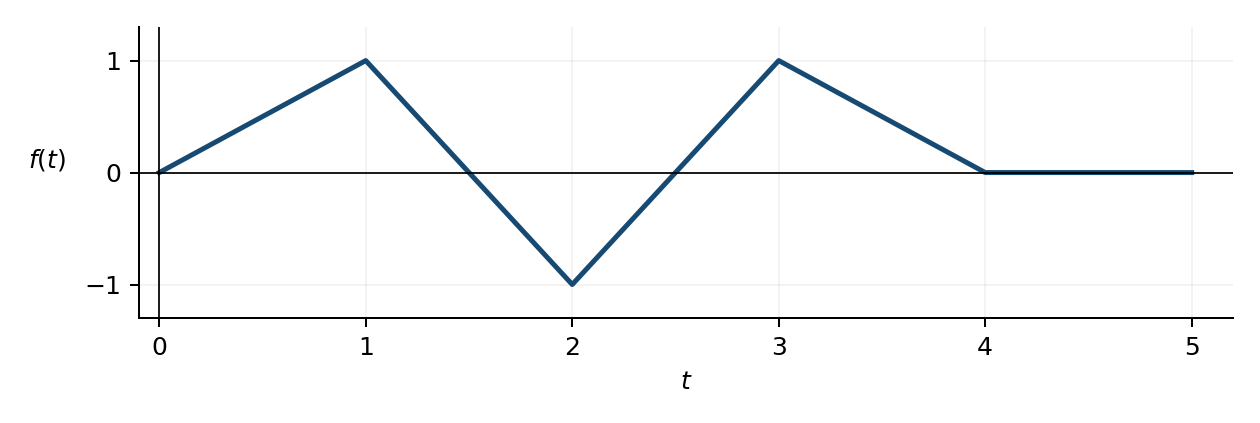
\includegraphics[width=.9\linewidth]{assets/M2-E0216-answer-graph.png}\end{center}

\noindent\textbf{(b)} $F(s)=(1-3e^{-s}+4e^{-2s}-3e^{-3s}+e^{-4s})/s^2$.

\noindent\textbf{(c)} Sea $R(t)=t-\sin t$ y $(c_0,c_1,c_2,c_3,c_4)=(1,-3,4,-3,1)$. Entonces
\[y(t)=\sin t+\sum_{j=0}^4c_jH(t-j)R(t-j).\]

\supportheading{answer}{M2-E0129}
\noindent\textbf{(a)} Sean \(r_\pm=(-5\pm\sqrt5)/2\),
\[h_0(t)=\frac{-r_-e^{r_+t}+r_+e^{r_-t}}{r_+-r_-},\quad h_1(t)=\frac{e^{r_+t}-e^{r_-t}}{r_+-r_-},\]
\(A=3/10100\), \(B=-3/1010\). La respuesta en metros es
\[x(t)=A\sin2t+B\cos2t-Bh_0(t)-2Ah_1(t).\]

\noindent\textbf{(b)} Usando \(h_0\),\(h_1\) del apartado anterior, define
\[R(t)=\frac{t-1+h_0(t)-h_1(t)}5.\]
La respuesta en metros es \(x(t)=.03[R(t)-R(t-10)u(t-10)]\), y su límite es 0.06 m.

\noindent\textbf{(c)} \[\zeta=\frac{c_2}{2\sqrt{m(k_1+k_3)}}=\frac{\sqrt5}{2}>1.\]
El sistema es sobreamortiguado.

\supportheading{answer}{M2-E0289}
$y(t)=\tfrac12[\sinh t+\sin t]$.

\supportheading{answer}{M2-E0040}
\noindent\textbf{(a)} \(f(t)=e^{4t}\).

\noindent\textbf{(b)} \(f(t)=\frac12t^2e^{4t}\).

\noindent\textbf{(c)} \(f(t)=\frac12(t-2)^2e^{4(t-2)}H(t-2)\).

\noindent\textbf{(d)} \(f(t)=\frac12t^2e^{4t}-(t-2)^2e^{4(t-2)}H(t-2)\).

\noindent\textbf{(e)} \(f(t)=\frac14(e^{3t}-e^{-t})\).

\noindent\textbf{(f)} \(f(t)=\frac14[e^{3t}-e^{-t}-H(t-2)(e^{3(t-2)}-e^{-(t-2)})]\).

\noindent\textbf{(g)} \(f(t)=\frac14e^{-t}-\frac14e^t+\frac12te^t\).

\noindent\textbf{(h)} \(f(t)=e^{-t}(\cos2t+\sin2t)\).

\noindent\textbf{(i)} \(f(t)=\frac14(e^{4t}-1)-\frac12H(t-2)(e^{4(t-2)}-1)\).

\noindent\textbf{(j)} \(f(t)=\sum_{n=0}^{\lfloor t\rfloor}(-1)^n e^{4(t-n)}\).

\noindent\textbf{(k)} \(f(t)=\sum_{n=0}^{\lfloor t/3\rfloor}2^n\sin(t-3n)\).

\Needspace{12\baselineskip}
\section*{Capítulo 7}
\addcontentsline{toc}{section}{Capítulo 7}
\supportheading{answer}{M2-E0290}
Con $X=(y,y',y'',y^{(3)})^T$:
\[X'=\begin{pmatrix}0&1&0&0\\0&0&1&0\\0&0&0&1\\-4&2&-3&0\end{pmatrix}X+\begin{pmatrix}0\\0\\0\\2e^{3t}\end{pmatrix}.\]

\supportheading{answer}{M2-E0238}
\[x_1=e^t(C_1\cos2t+C_2\sin2t),\qquad x_2=e^t(C_2\cos2t-C_1\sin2t),\quad C_1,C_2\in\mathbb R.\]

\supportheading{answer}{M2-E0064}
\[x_1=Ce^{2t}+De^{-t}+\frac32-e^t,\qquad x_2=-3De^{-t}+e^t.\]

\supportheading{answer}{M2-E0059}
\[x_2=e^{-2t}(C+Dt),\qquad x_1=e^{-2t}(D-2C-2Dt),\qquad C,D\in\mathbb R.\]

\supportheading{answer}{M2-E0344}
El monitor total informa de \(10\) en ambos ensayos, y el contador que reúne los dos sentidos registra \(10T\), también en ambos. El contador de A a B distingue las preparaciones para todo \(T>0\):
\[
C_{AB}^{\rm P}(T)=5T+\frac32(1-e^{-2T}),\qquad
C_{AB}^{\rm Q}(T)=5T-\frac32(1-e^{-2T}).
\]
La diferencia instantánea \(x_{\rm P}(T)-x_{\rm Q}(T)=6e^{-2T}\) tiende a cero, mientras la diferencia entre contadores direccionales tiende a \(3\). Cada contador direccional crece sin cota; lo finito es su diferencia histórica.

\supportheading{answer}{M2-E0047}
Con \(t\) en minutos y cantidades en kg,
\[A(t)=3e^{-0.04t}+2e^{-0.12t},\qquad B(t)=6e^{-0.04t}-4e^{-0.12t}.\]

\supportheading{answer}{M2-E0060}
\[\begin{aligned}
x_1&=Ce^{-2t}+D\cos4t+E\sin4t,\\
x_2&=-\tfrac C4e^{-2t}-\tfrac D2\sin4t+\tfrac E2\cos4t,\\
x_3&=-\tfrac C4e^{-2t}+D\cos4t+E\sin4t.
\end{aligned}\quad C,D,E\in\mathbb R.\]

\supportheading{answer}{M2-E0046}
\[x_1(t)=e^{2t}-\frac12-\frac12\cos(2t),\qquad
x_2(t)=e^{2t}-\frac12+\frac12\cos(2t),\quad t\in\mathbb R.\]

\supportheading{answer}{M2-E0065}
\noindent\textbf{(a)} \[X(t)=(I\cos t+A\sin t)C,\qquad C\in\mathbb R^2.\]

\noindent\textbf{(b)} \[X=C_1e^{-t}(0,1,-1)^T+C_2e^{3t}(2,3,3)^T+C_3e^{-2t}(-1,1,1)^T.\]

\noindent\textbf{(c)} \[X=C_1e^t(1,1,3)^T+e^{2t}\{C_2(1,0,1)^T+C_3(0,1,1)^T\}.\]

\noindent\textbf{(d)} \[X(t)=e^{2t}(I+tN)C,\qquad N=\begin{pmatrix}2&3&1\\-4&-6&-2\\8&12&4\end{pmatrix},\quad C\in\mathbb R^3.\]

\supportheading{answer}{M2-E0291}
Sea $\lambda_\pm=(3\pm\sqrt5)/2$. Entonces
\[x_1=C_+e^{\lambda_+t}+C_-e^{\lambda_-t}-3t-6,\]
\[x_2=(2-\lambda_+)C_+e^{\lambda_+t}+(2-\lambda_-)C_-e^{\lambda_-t}-3t-9.\]

\supportheading{answer}{M2-E0062}
\[x_1=C\cos t+D\sin t+2t-1,\qquad
x_2=C\sin t-D\cos t+t^2-2.\]

\supportheading{answer}{M2-E0070}
\[\omega_{1,2}=\sqrt{140\mp20\sqrt{29}}\ \mathrm{s}^{-1},\qquad
f_1\simeq .904481\ \mathrm{Hz},\quad f_2\simeq2.504875\ \mathrm{Hz}.\]

\supportheading{answer}{M2-E0066}
\noindent\textbf{(a)} \[X=C_1e^{2t}(1,2)^T+C_2e^{-4t}(1,-4)^T-\tfrac15e^t(1,1)^T.\]

\noindent\textbf{(b)} \[x_1=(C+Dt)e^{3t}+\frac t9+\frac2{27},\qquad
x_2=(3C+D+3Dt)e^{3t}+\frac19.\]

\supportheading{answer}{M2-E0067}
\[x_1=Ce^t+De^{-t}+5te^t,\qquad
x_2=(-C+3-5t)e^t-3De^{-t}.\]

\supportheading{answer}{M2-E0342}
El predictor simultáneo es \((S^*,I^*)=(0.72,0.13)\), y la corrección de Heun da
\[
(S_1,I_1)=(0.7132,0.1293).
\]
Con las mismas etapas, el incremento de retirados es
\[
\Delta R=\frac{0.5}{2}(0.1+0.13)=0.0575,
\qquad R_1=0.1575.
\]
La suma registrada disminuye de \(0.9\) a \(0.8425\), exactamente en \(0.0575\). Todos los estados iniciales, predictores y corregidos de este paso son no negativos y las tres fracciones suman uno.

\supportheading{answer}{M2-E0315}
\[
T_1'=-\tfrac12(T_1-T_2),\qquad T_2'=\tfrac13(T_1-T_2),\qquad 2T_1+3T_2=220.
\]
El predictor es \((62,32)\) y Heun da \((66.5,29)\,{}^\circ\mathrm C\). La referencia es
\[
T_1(t)=44+36e^{-5t/6},\qquad T_2(t)=44-24e^{-5t/6}.
\]
En \(t=0.6\), da aproximadamente \((65.8351,29.4433)\,{}^\circ\mathrm C\); conservar calor no elimina el error de aproximación.

\supportheading{answer}{M2-E0048}
Sea \(r=\sqrt7\), con \(t\) en minutos. Las cantidades, en kg, son
\[A(t)=200+e^{-t/20}\left[-200\cosh\frac{rt}{100}+\frac{400}{r}\sinh\frac{rt}{100}\right],\]
\[B(t)=200-\frac{600}{r}e^{-t/20}\sinh\frac{rt}{100}.\]

\supportheading{answer}{M2-E0343}
Escribiendo \(M_i=V_ic_i\), los balances son
\[
M_1'=5+5c_2-15c_1-k_1M_1,\qquad
M_2'=10+5c_1-25c_2-k_2M_2.
\]
Con los datos iniciales de limpieza,
\[
c_1'=0.1-0.4c_1+0.1c_2,\qquad
c_2'=0.1+0.05c_1-0.25c_2.
\]
En la concentración inicial común, las pendientes son \(0.04\) y \(0.06\,\mathrm{mg/(m^3\,min)}\), por lo que la igualdad no persiste. Para que persista desde cualquier valor común se necesitan
\[
\frac{s_1}{V_1}=\frac{s_2}{V_2},\qquad
\frac{Q_1}{V_1}+k_1=\frac{Q_2}{V_2}+k_2.
\]
Aquí basta establecer \(k_2=0.10\,\mathrm{min}^{-1}\). La concentración común satisface entonces \(c'=0.1-0.3c\), con \(c(0)=0.20\).

\supportheading{answer}{M2-E0063}
\[\begin{aligned}x_1&=Ce^t+D\sin t+E\cos t,\\x_2&=-Ce^t+D\cos t-E\sin t+t,\\x_3&=D\sin t+E\cos t+1.\end{aligned}\]

\supportheading{answer}{M2-E0061}
\[x_1=Ce^t+\frac{\cos t-\sin t}{4},\qquad
x_2=-3Ce^t-\frac{3\cos t+\sin t}{4},\quad C\in\mathbb R.\]
Solo hay una constante libre.

\supportheading{answer}{M2-E0369}
Los datos no determinan una única ley térmica ni unos parámetros numéricos. La respuesta debe conservar los dos datos iniciales y distinguir la temperatura medida en la carcasa de una temperatura media. El aumento inicial de la temperatura de la carcasa es compatible con una pérdida de energía total. El caso sencillo elegido y la simplificación deben justificarse mediante sus hipótesis, su comportamiento límite y una observación que permita contrastarlos; no hay un par obligatorio de modelos.

\supportheading{answer}{M2-E0049}
Con 40 pasos RK4 de tamaño \(h=0.025\),
\[x_1(1)\approx0.07734409109,\qquad x_2(1)\approx1.46444816554.\]
Son aproximaciones del modelo en sus unidades no especificadas; no son conteos de individuos ni cotas rigurosas de error.

\supportheading{answer}{M2-E0069}
Con \(N=\left(\begin{smallmatrix}2&-2&1\\2&-2&1\\-4&4&0\end{smallmatrix}\right)\),
\[X=e^t\left[(I+tN+\tfrac12t^2N^2)C+q(t)\right],\quad C\in\mathbb R^3,\]
\[q(t)=\begin{pmatrix}-t^5/15+t^4/3+t^2/2\\-t^5/15+t^4/3-t^3/3+t^2\\t- t^4/3+2t^3/3\end{pmatrix}.\]

\supportheading{answer}{M2-E0371}
El producto determina el par no ordenado \(\{\alpha,\beta\}=\{2,3\}\,\mathrm{min}^{-1}\), pero no su asignación. En \(t=\log2\), las dos asignaciones predicen \(b=1/4\) y \(b=3/8\). Sólo la primera pertenece al intervalo \([0.24,0.36]\); bajo el modelo resulta \(\alpha=2\), \(\beta=3\), y la primera etapa es la más lenta.

\supportheading{answer}{M2-E0359}
Entre cargas, para cantidades en mol y tiempo en min,
\[
a'=-ab,\qquad b'=-ab,\qquad p'=ab.
\]
En cada carga sólo \(b\) salta por la dosis añadida. Los resultados son
\[
\begin{array}{c|cc|c}
& p(1)\ (\mathrm{mol})&\max_{[0,1]}b\ (\mathrm{mol})&\text{cumple ambos criterios}\\\hline
\mathrm I&1.675052\ldots&2&\text{no}\\
\mathrm{II}&1.483806\ldots&1.279530\ldots&\text{sí}
\end{array}
\]
Con \(q=e^{-1}\), sea \(b_*=1+2q/(3-q)\) y \(r=e^{-1/2}b_* /(1+b_*)\). Entonces
\[
p_{\mathrm I}(1)=2-\frac{2q}{3-2q},
\qquad p_{\mathrm{II}}(1)=2-\frac r{1-r}.
\]
Ambos programas producirían finalmente \(2\,\mathrm{mol}\) si se dejara reaccionar indefinidamente; ese límite no determina el producto al minuto.

\supportheading{answer}{M2-E0068}
Con \(Y=(y,v,w)=(y,y',y'')\),
\[Y_{n+1}=Y_n+h(v_n,w_n,v_n^2-1-y_nw_n),\quad Y_0=(0,0,1.32824).\]
\[\begin{array}{c|rrrrr}t&0&0.5&1&1.5&2\\\hline
y_{h=.1}&0&.122927273&.484717769&.997774938&1.619960596\end{array}\]
En \(t=2\), las mallas \(h=.05,.025\) dan \(1.612449220\) y \(1.606896587\).
Son aproximaciones de primer orden, sin una cota fina de error certificada por estas tres mallas.

\supportheading{answer}{M2-E0045}
Para \(a\ne\pm1\),
\[x_1=Ce^{at}+De^{-t},\quad x_2=aCe^{at}-De^{-t},\quad
x_3=Ee^t-\frac{a^2C}{a-1}e^{at}+\frac D2e^{-t}.\]
Para \(a=1\), las dos primeras expresiones siguen siendo válidas y
\(x_3=(E-Ct)e^t+\tfrac D2e^{-t}\).
Para \(a=-1\),
\[x_1=(C+Dt)e^{-t},\quad x_2=(D-C-Dt)e^{-t},\quad
x_3=Ee^t+\left(\frac C2-\frac{3D}{4}+\frac{Dt}{2}\right)e^{-t}.\]
Las constantes \(C,D,E\) son reales y \(t\in\mathbb R\).

\supportheading{answer}{M2-E0362}
El balance es
\[
\frac{dV}{dt}=-Q,\qquad \frac{dm}{dt}=c_sQ-\lambda m,
\qquad Q=\frac{\alpha V}{R_0+\beta m},
\qquad (V(0),m(0))=(1\,\mathrm L,0),
\]
con \(c_s=1\,\mathrm{g/L}\) y \(\alpha=1\,\mathrm{kPa/L}\). Para los valores numéricos \(v=V/(1\,\mathrm L)\), \(z=m/(1\,\mathrm g)\), \(\tau=t/(1\,\mathrm{min})\), se obtiene
\[
v'=-\frac{v}{1+z},\qquad z'=\frac{v}{1+z}-z.
\]
Durante \(0\le\tau\le1/2\), \(v\ge e^{-\tau}>0.60\) y \(0\le z\le1-e^{-\tau}<0.40\). Sin embargo,
\[
v(1/2)\ge\left(\frac3{4e^{1/2}-1}\right)^{3/4}
=0.626610\ldots,
\]
de modo que se recogen como máximo \(0.373390\,\mathrm L<0.38\,\mathrm L\). El filtro de resistencia variable no cumple la producción. Dos pasos de Heun de \(0.25\,\mathrm{min}\) estiman \(0.34614\,\mathrm L\), sin constituir una cota de error.

El cartucho de resistencia constante sí cumple: \(v=e^{-\tau}\), \(z=\tau e^{-\tau}\), y recoge \(1-e^{-1/2}=0.393469\ldots\,\mathrm L\); sus mínimos y máximos relevantes son \(V_{\min}=0.606530\ldots\,\mathrm L\), \(m_{\max}=0.303265\ldots\,\mathrm g\).

\Needspace{12\baselineskip}
\section*{Capítulo 8}
\addcontentsline{toc}{section}{Capítulo 8}
\supportheading{answer}{M2-E0071}
\noindent\textbf{(a)} Impar en toda la recta.

\noindent\textbf{(b)} Par en toda la recta.

\noindent\textbf{(c)} Par en su dominio real \((-1,1)\).

\noindent\textbf{(d)} Ni par ni impar.

\noindent\textbf{(e)} Ni par ni impar.

\noindent\textbf{(f)} Impar en toda la recta.

\supportheading{answer}{M2-E0285}
$\|1\|=\sqrt{2\pi}$ y $\|\cos(nx)\|=\sqrt\pi$ para $n\ge1$. Todos los productos entre funciones distintas son cero.

\supportheading{answer}{M2-E0084}
\noindent\textbf{(a)} Son ortogonales: \(\langle f_1,f_2\rangle=0\).

\noindent\textbf{(b)} Son ortogonales: \(\langle f_1,f_2\rangle=0\).

\noindent\textbf{(c)} Son ortogonales: \(\langle f_1,f_2\rangle=0\).

\noindent\textbf{(d)} Son ortogonales: \(\langle f_1,f_2\rangle=0\).

\noindent\textbf{(e)} Son ortogonales: \(\langle f_1,f_2\rangle=0\).

\noindent\textbf{(f)} Son ortogonales: \(\langle f_1,f_2\rangle=0\).

\supportheading{answer}{M2-E0074}
\[f(x)=\frac12-\frac12\cos2x.\]
Es una serie finita y la igualdad vale para todo x.

\supportheading{answer}{M2-E0051}
\[|x|=\frac12-\frac4{\pi^2}\sum_{k=0}^{\infty}
\frac{\cos((2k+1)\pi x)}{(2k+1)^2},\qquad -1\le x\le1.\]
La suma es la extensión continua de período 2; en \(x=\pm1\) vale 1.

\supportheading{answer}{M2-E0293}
$\displaystyle S_N(x)=\frac4\pi\sum_{k=0}^{N-1}\frac{\sin((2k+1)x)}{2k+1}$. En los saltos la serie suma0.

\supportheading{answer}{M2-E0050}
\[S(x)=\frac{\sinh\pi}{\pi}\left[1+2\sum_{n=1}^{\infty}
\frac{(-1)^n}{1+n^2}\bigl(\cos nx-n\sin nx\bigr)\right].\]
En \(-\pi<x<\pi\), \(S(x)=e^x\); en \(x=\pm\pi\), \(S(x)=\cosh\pi\).
La suma se prolonga con período \(2\pi\).

\supportheading{answer}{M2-E0346}
Se anulan \(a_0\) y todos los coeficientes de índice par: \(a_{2m}=b_{2m}=0\), \(m\ge1\). La relación permite tanto senos como cosenos de índice impar.

No exige imparidad: \(f(t)=\cos t\) la satisface y es par. Tampoco exige periodo mínimo \(2\pi\): \(f(t)=\cos(3t)\) la satisface y tiene periodo mínimo \(2\pi/3\).

\supportheading{answer}{M2-E0072}
\[f(x)\sim\frac12+\frac2\pi\sum_{j=0}^\infty\frac{\sin((2j+1)\pi x)}{2j+1}.\]
La suma es f fuera de los enteros y vale1/2 en cada entero.

\supportheading{answer}{M2-E0052}
\noindent\textbf{(a)} \(a_0=2\pi^2/3\), \(a_n=4(-1)^n/n^2\), \(b_n=0\).

\noindent\textbf{(b)} \[\sum_{n=1}^{\infty}\frac{(-1)^{n+1}}{n^2}=\frac{\pi^2}{12}.\]

\noindent\textbf{(c)} \[\sum_{n=1}^{\infty}\frac1{n^2}=\frac{\pi^2}{6}.\]

\supportheading{answer}{M2-E0083}
\noindent\textbf{(a)} \[f(x)\sim-\frac4\pi\sum_{j=0}^{\infty}\frac{\sin((2j+1)\pi x)}{2j+1}.\]

\noindent\textbf{(b)} \[f(x)=\frac4\pi\sum_{n=1}^{\infty}\frac{\sin(n\pi/2)}{n^2}\sin(nx)
=\frac4\pi\sum_{j=0}^{\infty}\frac{(-1)^j}{(2j+1)^2}\sin((2j+1)x).\]

\noindent\textbf{(c)} \[f(x)=\frac8{\pi^3}\sum_{j=0}^{\infty}\frac{\sin((2j+1)\pi x)}{(2j+1)^3}.\]

\supportheading{answer}{M2-E0345}
En \([-L,L]\), las extensiones son
\[
F(x)=F_0\frac{x}{L}\left(1-\frac{|x|}{L}\right),\qquad
M(x)=F_0\frac{|x|}{L}\left(1-\frac{|x|}{L}\right),
\]
repetidas con periodo \(2L\). El registro con signo es impar y admite una serie de senos; el módulo es par y admite una serie de cosenos con término medio. Sus medias espaciales son \(0\) y \(F_0/6\), respectivamente. El primer coeficiente no nulo del registro con signo es
\[
b_1=\frac{8F_0}{\pi^3}.
\]
La reflexión invierte el signo de la componente, pero no el módulo.

\supportheading{answer}{M2-E0053}
\noindent\textbf{(a)} \[e^x=(e-1)+2\sum_{n=1}^{\infty}\frac{e(-1)^n-1}{1+n^2\pi^2}\cos(n\pi x),\quad0\le x\le1.\]

\noindent\textbf{(b)} \[\sin x=\frac2\pi+\frac4\pi\sum_{k=1}^{\infty}\frac{\cos(2kx)}{1-4k^2},\quad0\le x\le\pi.\]

\noindent\textbf{(c)} \[S(x)=\frac13+\sum_{n=1}^{\infty}\frac2{n\pi}
\left[\sin\frac{2n\pi}{3}-\sin\frac{n\pi}{3}\right]\cos\frac{n\pi x}{3}.\]
En el interior de cada tramo \(S=f\); \(S(1)=S(2)=1/2\), y \(S(0)=S(3)=0\).

\noindent\textbf{(d)} \[2x+1=4-\frac{24}{\pi^2}\sum_{k=1}^{\infty}
\frac{\cos((2k-1)\pi x/3)}{(2k-1)^2},\quad0\le x\le3.\]

\supportheading{answer}{M2-E0354}
La pareja compatible es \(\mathrm C\). Si sus amplitudes son \(a(t)\) y \(b(t)\),
\[
a(t)=U_0e^{-\gamma t},\qquad b(t)=U_0e^{-9\gamma t},
\qquad \gamma=\frac{\kappa\pi^2}{4L^2}.
\]
Cuando \(a=U_0/2\), la segunda amplitud conserva la fracción \(2^{-9}=1/512\) de su valor inicial. La tasa de decaimiento crece con el cuadrado del número de onda espacial; no es una frecuencia de oscilación temporal.

\supportheading{answer}{M2-E0292}
$\displaystyle S_N(x)=\frac2\pi\sum_{n=1}^N\frac{(-1)^{n+1}}n\sin(n\pi x)$. La serie converge a la rampa en el interior y a0 en sus saltos.

\supportheading{answer}{M2-E0082}
\noindent\textbf{(a)} Extensión2\ensuremath{\pi}-periódica de x en el interior y valor0 en \(x=(2k+1)\pi\).

\noindent\textbf{(b)} Extensión2\ensuremath{\pi}-periódica de |x|; en \(x=\pm\pi\) vale\ensuremath{\pi}.

\noindent\textbf{(c)} Extensión de período4: en0 vale1/2, en\ensuremath{\pm}2 vale3/2; en los intervalos abiertos conserva las fórmulas dadas.

\noindent\textbf{(d)} Extensión2\ensuremath{\pi}-periódica; suma0 en0 y \ensuremath{\pi}\ensuremath{^{2}}/2 en\ensuremath{\pm}\ensuremath{\pi}.

\noindent\textbf{(e)} Extensión de período2 de x\ensuremath{^{2}}, con valor1 en\ensuremath{\pm}1.

\noindent\textbf{(f)} Extensión de período\ensuremath{\pi} de x en(0,\ensuremath{\pi}), con valor\ensuremath{\pi}/2 en \(x=k\pi\).

\noindent\textbf{(g)} Extensión2\ensuremath{\pi}-periódica de \(e^x\), con valor \(\cosh\pi=(e^\pi+e^{-\pi})/2\) en\ensuremath{\pm}\ensuremath{\pi}.

\noindent\textbf{(h)} Extensión2\ensuremath{\pi}-periódica; valores en \((-\pi,-\pi/2,0,\pi/2,\pi)\): \((0,-1/2,0,1/2,0)\).

\supportheading{answer}{M2-E0347}
La mejor elección es
\[
g(t)=2+\sqrt6\cos(5t),\qquad \mathcal E(g)=3.
\]
Los aportes al error cuadrático medio de los cuatro términos de \(f\) son \(4,\,1/2,\,5/2,\,3\). Con dos unidades de presupuesto conviene conservar los dos mayores, que corresponden a la constante y al coseno de índice cinco.

\supportheading{answer}{M2-E0073}
\[f(x)\sim\frac\pi4-\frac2\pi\sum_{j=0}^{\infty}\frac{\cos((2j+1)x)}{(2j+1)^2}
+\sum_{n=1}^{\infty}\frac{(-1)^{n+1}}n\sin(nx).\]
La suma vale0 en x=0 y \ensuremath{\pi}/2 en x=\ensuremath{\pm}\ensuremath{\pi}; se extiende periódicamente.

\supportheading{answer}{M2-E0305}
En las fórmulas siguientes, $n\geq1$. Los coeficientes no indicados son cero. La suma coincide con la extensión periódica en sus puntos de continuidad.

\begin{enumerate}[label=(\alph*),ref=\alph*,leftmargin=*]
\item Con $k_n=n\pi/2$,
\[
C=\frac13,\qquad a_n=\frac{2(\sin k_n-k_n\cos k_n)}{k_n^3},\qquad b_n=0.
\]
La suma vale $0$ en $x=\pm1$ y $x=\pm2$, y en sus trasladados de período $4$.
\item Con $k_n=n\pi/3$,
\[
C=0,\qquad a_n=0,\qquad b_n=\frac23\left[\frac{\cos k_n-3(-1)^n}{k_n}-\frac{\sin k_n}{k_n^2}\right].
\]
La suma vale $-1/2$ en $x=-1$, $1/2$ en $x=1$ y $0$ en $x=\pm3$, con periodicidad $6$.
\item Con $k_n=n\pi/2$,
\[
C=\frac{17}{16},\qquad
a_n=\frac{(-1)^n-\cos(k_n/2)}{k_n^2},\qquad
b_n=\frac{(-1)^n}{2k_n}-\frac{\sin(k_n/2)}{k_n^2}.
\]
La suma vale $0$ en el vértice $x=1/2$ y $2$ en $x=\pm2$, con periodicidad $4$.
\item
\[
C=0,\qquad a_n=0,\qquad b_n=\frac{12(-1)^{n+1}}{n^3\pi^3}.
\]
La suma vale $0$ en $x=\pm1$ y sus trasladados de período $2$.
\item $C=1$, $a_2=1/2$, $a_4=-1/2$, $b_1=b_3=1$; todos los demás coeficientes son cero. La serie es finita y vale $1$ en $x=\pm\pi$.
\item $C=1$, $b_n=0$ y
\[
a_1=-\frac12,\qquad a_n=\frac{2(-1)^n}{1-n^2}\quad(n\geq2).
\]
La suma vale $0$ en $x=\pm\pi$ y sus trasladados de período $2\pi$.
\end{enumerate}

\supportheading{answer}{M2-E0349}
La construcción es posible exactamente cuando \(Q>4\). Todas las señales admisibles pueden escribirse
\[
f(t)=2+A\cos(2t+\phi)+B\cos(3t+\psi),
\]
con
\[
A>0,\quad B>0,\quad A^2+B^2=2(Q-4),
\]
y fases \(\phi,\psi\) libres módulo \(2\pi\). Ambos armónicos deben estar presentes para que el menor periodo sea \(2\pi\). Para \(Q=5\), sirve
\[
f(t)=2+\cos(2t)+\cos(3t).
\]
Si \(Q=4\), sólo queda la constante \(2\), que no cumple la condición de señal no constante; si \(Q<4\), los momentos son incompatibles.

\supportheading{answer}{M2-E0348}
El error cuadrático medio es
\[
E_N=\frac8{\pi^2}\sum_{j=N}^{\infty}\frac1{(2j+1)^2}
\le\frac4{\pi^2(2N-1)}.
\]
Por tanto, \(N=21\) términos garantizan \(E_N\le0.01\). En cambio, \(S_N(0)=0\) y \(f(0)=1\), así que el error puntual en cero siempre es uno. Reasignar \(f(0)=0\) anula ese error aislado sin alterar coeficientes ni \(E_N\), pero no produce un error uniformemente pequeño cerca del salto: en cualquier entorno de cero, el supremo del error sigue siendo al menos uno.

\Needspace{12\baselineskip}
\section*{Capítulo 9}
\addcontentsline{toc}{section}{Capítulo 9}
\supportheading{answer}{M2-E0316}
Para \(\lambda=0\), las autofunciones son todas las constantes no nulas. Las condiciones homogéneas dejan libre su escala; la normalización y la positividad seleccionan \(y(x)=1/2\).

\supportheading{answer}{M2-E0054}
\noindent\textbf{(a)} \[\lambda_n=\left(n+\frac12\right)^2\pi^2,\quad
y_n(x)=C\cos\left((n+\tfrac12)\pi x\right),\quad n=0,1,\ldots,\quad C\ne0.\]

\noindent\textbf{(b)} \(\lambda_0=0\), \(y_0=C\ne0\); para \(n\ge1\),
\(\lambda_n=n^2\pi^2\), \(y_n=C\cos(n\pi x)\), \(C\ne0\).

\supportheading{answer}{M2-E0353}
Los datos son compatibles tanto con
\[
X(0)=X(L)=0
\]
como con
\[
X'(0)=X'(L)=0.
\]
Las dos parejas mixtas quedan excluidas. Entre las dos parejas restantes, la comprobación de \(\lambda=0\) sí resuelve la duda: existe una autofunción constante no nula en el caso Neumann--Neumann y no existe una autofunción de autovalor cero en el caso Dirichlet--Dirichlet.

\supportheading{answer}{M2-E0297}
$\lambda_n=n^2$, $\phi_n=\sqrt{2/\pi}\sin(nx)$; $c_n=\sqrt{2\pi}(-1)^{n+1}/n$. Así $x=2\sum_{n\ge1}(-1)^{n+1}\sin(nx)/n$ para $0<x<\pi$ y en $L^2$. En ambos extremos la serie vale 0.

\supportheading{answer}{M2-E0350}
Las condiciones físicas son
\[
k_0u_x(0,t)=h_0u(0,t),\qquad
-2k_0u_x(L,t)=h_Lu(L,t).
\]
El problema espacial queda
\[
-\left[k_0\left(1+\frac{x}{L}\right)X'\right]'=\lambda c_0X,
\qquad k_0X'(0)=h_0X(0),\quad
2k_0X'(L)=-h_LX(L).
\]
Por tanto, \(p(x)=k_0(1+x/L)\), \(r(x)=0\), \(w(x)=c_0\). El problema es regular en \([0,L]\): \(p\) es continuamente derivable y positivo, y \(r,w\) son continuos con \(w>0\). El parámetro \(\lambda\) tiene unidades de tiempo inverso.

\supportheading{answer}{M2-E0085}
\noindent\textbf{(a)} \(s(x)=Ke^x\), \(K\ne0\); puede tomarse K=1. La ecuación es \(u^{\prime\prime}+\lambda u=0\).

\noindent\textbf{(b)} \[\lambda_n=n^2\pi^2,\qquad y_n(x)=C_ne^x\sin(n\pi x),\quad n=1,2,\ldots,\ C_n\ne0.\]

\noindent\textbf{(c)} Los mismos \(\lambda_n=n^2\pi^2\) y \(y_n=C_ne^x\sin(n\pi x)\).

\supportheading{answer}{M2-E0351}
La forma regular es
\[
-(xy')'=\lambda\frac1x y,
\qquad p=x,\quad r=0,\quad w=\frac1x.
\]
El producto adecuado es \(\langle f,g\rangle_w=\int_1^e fg\,dx/x\). Para el par dado,
\[
\int_1^e\frac{uv}{x}\,dx=0,\qquad
\int_1^e uv\,dx
=-\frac{4\pi^2(e+1)}{(1+\pi^2)(1+9\pi^2)}\ne0.
\]
Con \(z=\log x\), la medida ponderada se convierte en \(dz\); la no ponderada conserva el factor \(e^z\).

\supportheading{answer}{M2-E0055}
\noindent\textbf{(a)} Para \(n=1,2,\ldots\), \(k_n=(n-\tfrac12)\pi\),
\(\lambda_n=k_n^2\), \(y_n=C\sin(k_nx)\), \(C\ne0\).

\noindent\textbf{(b)} \(\phi_n(x)=\sqrt2\sin(k_nx)\), con \(\int_0^1\phi_n^2dx=1\).

\noindent\textbf{(c)} \[1=\sum_{n=1}^{\infty}\frac{2}{k_n}\sin(k_nx),\quad0<x\le1.\]
En la base normalizada el coeficiente es \(\sqrt2/k_n\).
La igualdad vale en \(L^2(0,1)\); la suma es 0 en x=0.

\noindent\textbf{(d)} \[c_n=\frac{2\sqrt2\sin(k_n/2)}{k_n^2},\qquad
f(x)=\sum_{n=1}^{\infty}\frac{4\sin(k_n/2)}{k_n^2}\sin(k_nx),\quad0\le x\le1.\]

\supportheading{answer}{M2-E0239}
\[\lambda_0=-1,\quad y_0(x)=C_0e^{-x};\qquad \lambda_n=n^2\pi^2,\quad y_n(x)=C_n[\sin(n\pi x)-n\pi\cos(n\pi x)],\ n\ge1.\]
Cada constante multiplicativa es no nula. Cero no es autovalor.

\supportheading{answer}{M2-E0087}
\noindent\textbf{(a)} Sean \(\mu_n\in((n-1)\pi,(n-1)\pi+\pi/2)\) las raíces de \(\mu_n\tan\mu_n=1\), n\ensuremath{\ge}1.
\[\lambda_n=\mu_n^2,\qquad \phi_n(x)=d_n\cos(\mu_nx),\quad d_n=\sqrt{\frac2{1+\sin^2\mu_n}}.\]

\noindent\textbf{(b)} \[1-x=\sum_{n=1}^{\infty}c_n\phi_n(x),\qquad
c_n=\frac{d_n(1-\cos\mu_n)}{\mu_n^2}.\]

\noindent\textbf{(c)} \[f\sim\sum_{n=1}^{\infty}c_n\phi_n,\qquad
c_n=\frac{d_n\sin(\mu_n/2)}{\mu_n}.\]
La suma vale1/2 en x=1/2; en los puntos de continuidad coincide con f.

\supportheading{answer}{M2-E0241}
Con $a_n=(n-1)\pi$ y $n\to\infty$,
\[\mu_n=a_n+\frac1{a_n}+O(a_n^{-3}),\qquad\lambda_n=a_n^2+2+O(a_n^{-2})\sim(n-1)^2\pi^2.\]

\supportheading{answer}{M2-E0086}
\noindent\textbf{(a)} Todos los autovalores son reales y estrictamente positivos.

\noindent\textbf{(b)} \(\lambda=0\), \(y=C(1-x)\), C\ensuremath{\ne}0; los demás autovalores son positivos.

\noindent\textbf{(c)} Existe una única \(\mu>0\) con \(\alpha=\mu\coth\mu\).
El autovalor negativo es \(\lambda_-=-\mu^2\), con \(y=C\sinh(\mu(1-x))\).
Los positivos son k\ensuremath{^{2}} con \(\alpha\sin k-k\cos k=0\), k>0.

\supportheading{answer}{M2-E0240}
Todos los autovalores son positivos: $\lambda_n=k_n^2$, donde $k_n$ es la única raíz de
\[\tan(\pi k_n)=-k_n,\qquad n-\tfrac12<k_n<n,\quad n=1,2,\ldots.\]
Las autofunciones son $C_n\sin(k_nx)$, $C_n\ne0$. Cero no es autovalor. Si $m_n=n-\tfrac12$,
\[k_n=m_n+\frac1{\pi m_n}+O(m_n^{-3}),\qquad\lambda_n=m_n^2+\frac2\pi+O(m_n^{-2})\sim\frac{(2n-1)^2}{4}.\]

\supportheading{answer}{M2-E0056}
Existe solución para todo \(a\in\mathbb R\), y todas son
\[y(x)=\frac a{\pi^2}+C\cos(\pi x),\qquad C\in\mathbb R.\]

\supportheading{answer}{M2-E0242}
Sean $k_n\in((n-\tfrac12)\pi,n\pi)$ las raíces de $\tan k_n=-k_n$, $n\ge1$. La solución única es
\[y(x)=\sum_{n=1}^\infty\frac{4\sin k_n}{k_n^2(k_n^2-2)(1+\cos^2k_n)}\sin(k_nx).\]
Como comprobación, con $r=\sqrt2$,
\[y(x)=-\frac x2+\frac{\sin(rx)}{\sin r+r\cos r}.\]

\supportheading{answer}{M2-E0088}
Solo \(a=0\). En ese caso,
\[y(x)=C\sin\pi x-\frac{x}{2\pi}\sin\pi x,\quad C\in\mathbb R.\]

\supportheading{answer}{M2-E0243}
\[y(x)=8\sum_{n=1}^\infty\frac{\sin(n\pi/2)}{n^2\pi^2(n^2\pi^2-2)}\sin(n\pi x).\]
Equivalentemente, para $r=\sqrt2$,
\[y(x)=\begin{cases}-x+\dfrac{\sin(rx)}{r\cos(r/2)},&0\le x\le1/2,\\-(1-x)+\dfrac{\sin(r(1-x))}{r\cos(r/2)},&1/2\le x\le1.\end{cases}\]

\supportheading{answer}{M2-E0089}
No existen autovalores reales: para todo \(\lambda\in\mathbb R\), la única solución es y=0.

\supportheading{answer}{M2-E0244}
\[y(x)=\frac18-\sum_{n=1}^\infty\frac{2[1-\cos(n\pi/2)]}{n^2\pi^2(n^2\pi^2-1)}\cos(n\pi x).\]
Una forma cerrada equivalente es
\[y(x)=\frac12-x+A\cos x+\sin x+H(x-\tfrac12)[x-\tfrac12-\sin(x-\tfrac12)],\qquad A=\frac{\cos1-\cos(1/2)}{\sin1}.\]

\supportheading{answer}{M2-E0352}
Para \(0<\delta<1\), la solución única es
\[
y_{\delta,\varepsilon}(x)=\frac{\sin(2x)}{3+\delta}
+\frac{\varepsilon}{\delta}\sin x.
\]
Las dos familias convergen uniformemente en \([0,\pi]\) a
\[
\varepsilon=\delta:\quad \frac13\sin(2x)+\sin x,
\qquad
\varepsilon=\delta^2:\quad \frac13\sin(2x).
\]
El problema límite tiene todas las soluciones \(\frac13\sin(2x)+C\sin x\), \(C\in\mathbb R\). No selecciona una única aproximación para ambas familias: aunque \(\varepsilon\) desaparece, el cociente \(\varepsilon/\delta\) determina una amplitud que puede persistir.

\Needspace{12\baselineskip}
\section*{Capítulo 10}
\addcontentsline{toc}{section}{Capítulo 10}
\supportheading{answer}{M2-E0252}
$u(x,y)=F(y)-xy$, con $F$ arbitraria de clase $C^1$.

\supportheading{answer}{M2-E0254}
$u(x,y)=xy^2+F(x)$, con $F$ arbitraria de clase $C^1$.

\supportheading{answer}{M2-E0260}
$u(x,y)=A(y)e^{-x}$, con $A$ arbitraria de clase $C^1$.

\supportheading{answer}{M2-E0258}
$u(x,y)=A(y)+B(y)e^{-x}+xy$, con $A,B$ arbitrarias de clase $C^2$.

\supportheading{answer}{M2-E0262}
$u(x,y)=1+\dfrac y8(1-2x+2x^2-e^{-2x})$.

\supportheading{answer}{M2-E0381}
Las condiciones son \(T_x(0,t)=0\) y \(kT_x(L,t)=P/A\). Se obtiene \(E'(t)=P\), así que no puede haber un estado estacionario con estas hipótesis y P>0. Fijar potencia impone flujo; fijar temperatura impone otro tipo de condición y deja que el flujo resultante dependa de la solución.

\supportheading{answer}{M2-E0264}
\[u(x,t)=\frac4\pi\sum_{j=1}^{\infty}\frac{(-1)^{j+1}}{(2j-1)^2}e^{-2(2j-1)^2t}\sin((2j-1)x).\]

\supportheading{answer}{M2-E0107}
\[u(x,t)=\frac{\sin(ct)}c\cos x.\]
Para ct=0,\ensuremath{\pi}/2,\ensuremath{\pi},3\ensuremath{\pi}/2, los perfiles son respectivamente0,cosx/c,0,\ensuremath{-}cosx/c.
El período temporal fundamental es2\ensuremath{\pi}/c.

\supportheading{answer}{M2-E0057}
\noindent\textbf{(a)} \[u(x,t)=\frac12-\frac4{\pi^2}\sum_{j=0}^{\infty}
\frac{e^{-k(2j+1)^2\pi^2t}\cos((2j+1)\pi x)}{(2j+1)^2}.\]

\noindent\textbf{(b)} \(u_{\rm eq}(x)=1/2\), constante.

\supportheading{answer}{M2-E0273}
\[u(x,t)=\cos\frac{\alpha\pi t}{L}\sin\frac{\pi x}{L}+\cos\frac{3\alpha\pi t}{L}\sin\frac{3\pi x}{L},\qquad T=\frac{2L}{\alpha}.\]

\supportheading{answer}{M2-E0355}
Se tiene \(r=1/4\). En orden \(j=1,2,3\), los valores interiores, en kelvin de exceso, son
\[
(U_1^1,U_2^1,U_3^1)=(2+2\sqrt2,\ 4+2\sqrt2,\ 2+2\sqrt2),
\]
\[
(U_1^2,U_2^2,U_3^2)=\left(2+\frac{3\sqrt2}{2},\ 3+2\sqrt2,\ 2+\frac{3\sqrt2}{2}\right).
\]
En el segundo paso, los valores exactos son aproximadamente \((4.155542,\ 5.876824,\ 4.155542)\,\mathrm K\). El máximo error nodal absoluto es \(0.04839643\,\mathrm K\), en el nodo central.

\supportheading{answer}{M2-E0108}
\noindent\textbf{(a)} \[u(x,t)=\frac{400}\pi\sum_{j=0}^{\infty}\frac{1}{2j+1}
\sin\frac{(2j+1)\pi x}{20}\exp\left[-\frac{(2j+1)^2\pi^2kt}{400}\right].\]

\noindent\textbf{(b)} \[u_2(10,30)=\frac{400}\pi\left[e^{-30k\pi^2/400}-\frac13e^{-270k\pi^2/400}\right].\]
Plata:35.907441°C; aluminio:67.228413°C; hierro:97.421140°C.

\supportheading{answer}{M2-E0277}
\[u(x,t)=\frac{L}{3\pi\alpha}\sin\frac{3\pi\alpha t}{L}\sin\frac{3\pi x}{L},\qquad T=\frac{2L}{3\alpha}.\]

\supportheading{answer}{M2-E0276}
\[u(x,t)=\frac12\left[\frac1{1+(x-\alpha t)^2}+\frac1{1+(x+\alpha t)^2}\right].\]

\supportheading{answer}{M2-E0109}
\noindent\textbf{(a)} \[u(x,y)=\sum_{n=1}^{\infty}b_n\frac{\sinh(n\pi y/a)}{\sinh(n\pi b/a)}\sin\frac{n\pi x}{a},\qquad
b_n=\frac2a\int_0^a g(s)\sin\frac{n\pi s}{a}ds.\]

\noindent\textbf{(b)} \[u(x,y)=\frac{4a}{\pi^2}\sum_{n=1}^{\infty}\frac{\sin(n\pi/2)}{n^2}
\frac{\sinh(n\pi y/a)}{\sinh(n\pi b/a)}\sin\frac{n\pi x}{a}.\]

\supportheading{answer}{M2-E0358}
Con la regularidad exigida, el primer registro es compatible con la cuerda. Una solución que lo demuestra es
\[
u(x,t)=\sin(\pi x/L)\cos(c\pi t/L).
\]
El calor exigiría \(u_t(x,0)=-\kappa(\pi/L)^2\sin(\pi x/L)\), y el equilibrio con ambos extremos nulos sólo admite \(U=0\); ninguno coincide con el registro completo.

En el segundo registro queda descartada la continuidad en todo el rectángulo cerrado. La clase que sólo impone el límite inicial en cada punto interior no queda descartada por ese argumento de esquina. El desacuerdo inicial de extremos no permite concluir que todo modelo térmico para \(t>0\) sea imposible; tampoco la ausencia de esa contradicción constituye por sí sola una prueba general de existencia.

\supportheading{answer}{M2-E0270}
\[u(x,t)=\frac{e^\pi-1}{\pi}+\sum_{n=1}^{\infty}\frac{2[e^\pi(-1)^n-1]}{\pi(1+n^2)}e^{-n^2t}\cos(nx).\]

\supportheading{answer}{M2-E0356}
El sistema es
\[
4A-B-C=23,\qquad 4B-A-D=43,
\]
\[
4C-A-D=15,\qquad 4D-B-C=35.
\]
Su solución es \((A,B,C,D)=(13,18,11,16)\). Son los valores de \(H\) en los cuatro nodos interiores. El polinomio es armónico, coincide con los datos de contorno de la tabla y sus diferencias segundas son exactas. Este acuerdo es propio de la referencia y la malla dadas; no establece error nulo en problemas generales ni determina valores de contorno entre los nodos.

\supportheading{answer}{M2-E0272}
\[u(x,t)=\sum_{j=1}^{\infty}\frac{400}{(2j-1)\pi}\exp\!\left[-\alpha^2\left(\frac{(2j-1)\pi}{2L}\right)^2t\right]\sin\frac{(2j-1)\pi x}{2L}.\]

\supportheading{answer}{M2-E0300}
\noindent\textbf{(a)} Sea $f_0=a^{-1}\int_0^af(s)\,ds$ y, para $n\geq1$,
$f_n=(2/a)\int_0^af(s)\cos(n\pi s/a)\,ds$, $\kappa_n=n\pi/a$.
Entonces
\[
u(x,y)=f_0(1-y/b)+\sum_{n=1}^{\infty}
f_n\frac{\sinh(\kappa_n(b-y))}{\sinh(\kappa_nb)}\cos(\kappa_nx).
\]

\noindent\textbf{(b)} Con $f_0,f_n$ como en el apartado anterior y
$g_0=a^{-1}\int_0^ag(s)\,ds$,
$g_n=(2/a)\int_0^ag(s)\cos(n\pi s/a)\,ds$,
\[
u=f_0(1-y/b)+g_0y/b+\sum_{n=1}^{\infty}
\left[f_n\frac{\sinh(\kappa_n(b-y))}{\sinh(\kappa_nb)}
+g_n\frac{\sinh(\kappa_n y)}{\sinh(\kappa_nb)}\right]\cos(\kappa_nx),
\qquad \kappa_n=\frac{n\pi}{a}.
\]

\noindent\textbf{(c)} \[
u(x,y)=\frac{\sinh(1-y)}{\sinh1}\cos x
+\frac{\sinh(2y)}{\sinh2}\cos2x
-\frac{\sinh(3(1-y))}{\sinh3}\cos3x.
\]

\supportheading{answer}{M2-E0268}
\[u(x,t)=200\left(1-\frac x\pi\right)-\sum_{n=1}^{\infty}\frac{400}{n\pi}e^{-n^2t}\sin(nx).\]

\supportheading{answer}{M2-E0257}
$u(x,y)=A(y)+B(y)e^{-2x}+\frac y2(x^2-x)$, con $A,B$ arbitrarias de clase $C^2$.

\supportheading{answer}{M2-E0294}
$u=5e^{4yx}+3(e^{4yx}-1)/(4y)$ si $y\ne0$, y $u(x,0)=5+3x$.

\supportheading{answer}{M2-E0265}
\[u(x,t)=e^{-2t}\sin x+\sum_{n=1}^{\infty}\frac{4(-1)^{n+1}}{n^3}(1-e^{-2n^2t})\sin(nx).\] Equivalentemente, si $q(x)=(\pi^2x-x^3)/3$, \[u=q-3e^{-2t}\sin x+\sum_{n=2}^{\infty}\frac{4(-1)^n}{n^3}e^{-2n^2t}\sin(nx).\]

\supportheading{answer}{M2-E0256}
$u(x,y)=x^2+F(x)e^{-y^2}+G(y)$, con funciones arbitrarias de clase $C^2$.

\supportheading{answer}{M2-E0275}
\[\begin{split}u(x,t)={}&\cos(\alpha t)\sin x+\frac5{2\alpha}\sin(2\alpha t)\sin(2x)-\frac3{5\alpha}\sin(5\alpha t)\sin(5x)\\&+\sum_{n=1}^{\infty}\frac{2(-1)^{n+1}}{\alpha^2n^3}\left[t-\frac{\sin(\alpha nt)}{\alpha n}\right]\sin(nx).\end{split}\]

\supportheading{answer}{M2-E0261}
$u(x,y)=\dfrac y2+F(y)e^{-2x}+G(x)$, con $F,G$ arbitrarias de clase $C^2$.

\supportheading{answer}{M2-E0106}
\noindent\textbf{(a)} \[u(x,t)=\sum_{n=1}^{\infty}B_n\cos\frac{cn\pi t}{L}\sin\frac{n\pi x}{L},\qquad
B_n=\frac{2h_0L^2}{a(L-a)n^2\pi^2}\sin\frac{n\pi a}{L}.\]

\noindent\textbf{(b)} \[\omega_n=\frac{cn\pi}{L},\qquad f_n=\frac{cn}{2L},\quad n=1,2,\ldots.\]
El principal corresponde a n=1 y tiene período2L/c.

\supportheading{answer}{M2-E0259}
$u(x,y)=[A(y)+xB(y)]e^{-x}+y(x-2)$, con $A,B$ arbitrarias de clase $C^2$.

\supportheading{answer}{M2-E0274}
\[u(x,t)=\frac{2V_0L^3}{\alpha a(L-a)\pi^3}\sum_{n=1}^{\infty}\frac{\sin(n\pi a/L)}{n^3}\sin\frac{\alpha n\pi t}{L}\sin\frac{n\pi x}{L}.\]

\supportheading{answer}{M2-E0267}
El modelo es $u_t=u_{xx}+5$, $u(0,t)=u(\pi,t)=0$, $u(x,0)=25$ en el interior. Con $q(x)=\frac52x(\pi-x)$, \[u(x,t)=q(x)+\sum_{\substack{n\ge1\\n\text{ impar}}}\left(\frac{100}{n\pi}-\frac{20}{n^3\pi}\right)e^{-n^2t}\sin(nx).\]

\supportheading{answer}{M2-E0253}
Para $x\ne0$, $u=[F(y)+2ye^{2x}]/x$. Una solución de clase $C^1$ que atraviesa $x=0$ necesariamente tiene $F(y)=-2y$ y \[u(x,y)=2y\frac{e^{2x}-1}{x}\quad(x\ne0),\qquad u(0,y)=4y.\]

\supportheading{answer}{M2-E0299}
\noindent\textbf{(a)} \[
u(x,t)=\sum_{n=1}^{\infty}F_n\cos(\beta_nt)\sin\frac{n\pi x}{L},
\qquad F_n=\frac2L\int_0^Lf(s)\sin\frac{n\pi s}{L}\,ds,\]
\[\beta_n=\sqrt{\alpha^2(n\pi/L)^2+k}.
\]

\noindent\textbf{(b)} \[
u(x,t)=\sum_{n=1}^{\infty}\frac{G_n}{\beta_n}\sin(\beta_nt)
\sin\frac{n\pi x}{L},\qquad
G_n=\frac2L\int_0^Lg(s)\sin\frac{n\pi s}{L}\,ds,\]
\[\beta_n=\sqrt{\alpha^2(n\pi/L)^2+k}.
\]

\supportheading{answer}{M2-E0255}
Una forma válida también en $x=0$ es \[u(x,y)=A(x)y+B(x)+S(x,y),\quad S(x,y)=\begin{cases}[\sin(xy)-xy]/x^2,&x\ne0,\\0,&x=0,\end{cases}\] con $A,B$ arbitrarias de clase $C^2$. En $x\ne0$ equivale a $F(x)+yG(x)+\sin(xy)/x^2$.

\supportheading{answer}{M2-E0263}
$u(x,t)=1+(e^{-t}-1)e^{x/3}$.

\supportheading{answer}{M2-E0269}
\[u(x,t)=\sum_{n=1}^{\infty}\frac{8(-1)^{n+1}-4}{n^3\pi^3}e^{-5n^2\pi^2t}\sin(n\pi x).\]

\supportheading{answer}{M2-E0379}
Con \(r=0.6\), el primer paso es \((-2,6)\,\mathrm K\). El mayor paso que conserva no negatividad para todos los datos no negativos es \(\Delta t=0.5\,\mathrm s\). En la malla fija, los dos multiplicadores con el paso de \(0.6\,\mathrm s\) son \(0.4\) y \(-0.8\), por lo que toda perturbación inicial decae aunque pueda aparecer una temperatura negativa. Ninguna de esas garantías cuantifica por sí sola el error respecto de la solución continua.

\supportheading{answer}{M2-E0266}
\noindent\textbf{(a)} \[f(x)=\begin{cases}2x,&0\le x\le50,\\2(100-x),&50\le x\le100,\end{cases}\quad[{}^\circ\mathrm C].\]

\noindent\textbf{(b)} \[u(x,t)=20-\frac x5+\sum_{n=1}^{\infty}\left[\frac{800\sin(n\pi/2)}{n^2\pi^2}-\frac{40}{n\pi}\right]e^{-1.14(n\pi/100)^2t}\sin\frac{n\pi x}{100}.\]

\supportheading{answer}{M2-E0271}
\[u(x,t)=100-\frac{3200}{\pi^3}\sum_{j=1}^{\infty}\frac{e^{-3(2j-1)^2t}}{(2j-1)^3}\sin((2j-1)x).\]

\supportheading{answer}{M2-E0380}
La malla gruesa da \(2.50000\,\mathrm K\) en el centro. Al refinar, conservar \(\Delta t=0.25\,\mathrm s\) da \(r=1\) y un modo con multiplicador de módulo mayor que uno. Para conservar \(r=1/4\), tome \(\Delta t=0.0625\,\mathrm s\); ocho pasos dan \(2.81738\,\mathrm K\). La referencia es \(2.91213\,\mathrm K\): los errores son aproximadamente \(0.41213\,\mathrm K\) y \(0.09475\,\mathrm K\). Sólo el cálculo refinado satisface la tolerancia dada.

\supportheading{answer}{M2-E0058}
\[u(x,0)=\frac{e^{-x^2}}{2c}+C,\qquad
u(x,t)=\frac{e^{-(x-ct)^2}}{2c}+C,\quad C\in\mathbb R.\]
Si además se impone desplazamiento nulo en el infinito, \(C=0\).

\supportheading{answer}{M2-E0357}
Si \(a=\kappa\pi^2/L^2\), el problema transformado es
\[
\kappa U_{xx}-sU=-\Theta\left[3\sin(\pi x/L)-\sin(2\pi x/L)\right],
\qquad U(0,s)=U(L,s)=0.
\]
Para cada \(s>0\), su solución única es
\[
U(x,s)=\frac{3\Theta}{s+a}\sin(\pi x/L)
-\frac{\Theta}{s+4a}\sin(2\pi x/L).
\]
La inversión da
\[
u(x,t)=3\Theta e^{-at}\sin(\pi x/L)
-\Theta e^{-4at}\sin(2\pi x/L).
\]
Esta función satisface la EDP y todos los datos; sus transformadas y las de las derivadas utilizadas existen para \(s>0\).

\chapter{Soluciones de consulta}
\Needspace{12\baselineskip}
\section*{Capítulo 1}
\addcontentsline{toc}{section}{Capítulo 1}
\supportheading{solution}{M2-E0103}
\noindent\textbf{Resultado.} $y=2(1+Ce^{4x})/(1-Ce^{4x})$ donde $1-Ce^{4x}\ne0$, junto con $y=-2$. El caso $C=0$ ya da $y=2$.

\noindent\textit{Desarrollo.} Los equilibrios satisfacen $y^2-4=0$: son $y=\pm2$. Fuera de ellos, separar e integrar da $\tfrac14\ln|(y-2)/(y+2)|=x+K$. Al absorber el signo en una constante real se obtiene $(y-2)/(y+2)=Ce^{4x}$ y la familia indicada. Si $C<0$, el denominador es positivo y la solución está definida en toda $\mathbb R$, entre $-2$ y $2$. Si $C>0$, hay un polo en $x_*=-\ln C/4$ y los intervalos máximos son $(-\infty,x_*)$ y $(x_*,\infty)$. Si $C=0$, la solución es el equilibrio $2$, y el equilibrio $-2$ se añade por separado. Con $z=Ce^{4x}$, la derivada de la familia es $16z/(1-z)^2$, y también $y^2-4=16z/(1-z)^2$. El campo es suave; no existen empalmes de soluciones distintas en puntos finitos de los equilibrios.

\supportheading{solution}{M2-E0025}
\noindent\textbf{(a) Resultado.} $T^{\prime}=-k(T-20)$ con $k>0$; $k$ se mide en $\mathrm{min}^{-1}$.

\noindent\textit{Desarrollo.} Si la capacidad calorífica total es $C_H>0$ y la potencia de salida es $H(T-20)$, con $H>0$, el balance es $C_HT^{\prime}=-H(T-20)$. Con $k=H/C_H>0$ resulta el modelo indicado. Si $T>20$, la derivada es negativa; si $T<20$, el signo se invierte y el entorno calienta el cuerpo. En la convención $T^{\prime}=\alpha(T-20)$, la constante sería $\alpha=-k<0$.

\medskip

\noindent\textbf{(b) Resultado.} $T(60)=22.8125\,{}^\circ\mathrm C$; el descenso desde el minuto 30 es $12.1875\,{}^\circ\mathrm C$.

\noindent\textit{Desarrollo.} Separar da $T=20+80e^{-kt}$. El dato de 30 minutos impone $e^{-30k}=15/80=3/16$, luego $k=\ln(16/3)/30\ \mathrm{min}^{-1}$. Por tanto $T(60)=20+80(3/16)^2=20+45/16=22.8125$. El descenso en ese intervalo es $35-T(60)=195/16=12.1875$. El dato inicial y el de calibración se recuperan al sustituir. La temperatura desciende hacia 20 sin cruzarlo; el segundo descenso es menor que el primero, de acuerdo con la menor diferencia térmica.

\supportheading{solution}{M2-E0032}
\noindent\textbf{Resultado.} $h(t)=24-\dfrac4{15}t$ cm para $0\le t<90$ días; el vaciado se alcanza en $t=90$ días.

\noindent\textit{Desarrollo.} La sección horizontal de la esfera a altura h tiene radio cuadrado $16^2-(h-16)^2=h(32-h)$, de modo que su área es $A(h)=\pi h(32-h)$. También $dV/dh=32\pi h-\pi h^2=A(h)$, como debe ocurrir al añadir una lámina de espesor dh. Si k>0 es la constante de evaporación, con unidades cm/día, el balance es $dV/dt=-kA(h)$. Por la regla de la cadena, $A(h)h^{\prime}=-kA(h)$. Mientras $0<h<32$, A es positiva y $h^{\prime}=-k$. Integrar da $h=24-kt$. El dato $h(15)=20$ fija $k=4/15$ cm/día. La solución conserva ambas alturas y el balance de volumen; llega a h=0 en 90 días. En ese extremo A=0 y la cancelación anterior ya no procede; prolongar la recta produciría alturas negativas ajenas al modelo.

\supportheading{solution}{M2-E0191}
\noindent\textbf{Resultado.} Además de $y\equiv0$, para cada $a\ge0$ y $\sigma\in\{-1,1\}$:
\[y(x)=\begin{cases}0,&x\le a,\\ \sigma[\tfrac23(x-a)]^{3/2},&x>a.\end{cases}\]

\noindent\textit{Desarrollo.} El campo $\sqrt[3]{y}$ es continuo, por lo que existe solución local. No es localmente Lipschitz en $y=0$. La función nula y las dos ramas que salen en $a=0$ ya prueban que no hay unicidad. Para obtener todas las ramas no nulas, derivamos $|y|^{2/3}$: en cualquier intervalo donde $y\ne0$, su derivada es $2/3$. Así $|y|^{2/3}=\frac23(x-a)$, necesariamente con $x>a$, y el signo de $y$ es constante. Una rama no nula no puede regresar a cero hacia adelante; antes de salir del cero sólo puede permanecer en él. Como $y(0)=0$, la salida debe satisfacer $a\ge0$. En el empalme, tanto $y$ como $y'$ tienden a cero, y la fórmula por tramos es $C^1$ y cumple la EDO en todo punto. Permitir cualquier tiempo de espera, o no salir nunca, completa la familia.

\Needspace{12\baselineskip}
\section*{Capítulo 2}
\addcontentsline{toc}{section}{Capítulo 2}
\supportheading{solution}{M2-E0196}
\noindent\textbf{Resultado.} $y(x)=\tfrac13e^{-x}+e^{-4x}$, $x\in\mathbb R$.

\noindent\textit{Desarrollo.} El factor integrante es $e^{4x}$, de modo que $(e^{4x}y)'=e^{3x}$. Integrar da $y=\frac13e^{-x}+Ce^{-4x}$. El dato inicial determina $C=1$. Al derivar y sumar $4y$, el término $e^{-4x}$ se cancela y queda $e^{-x}$; en cero la suma es $4/3$. Los coeficientes continuos garantizan unicidad en toda la recta.

\supportheading{solution}{M2-E0021}
\noindent\textbf{Resultado.} $y=0$ y las ramas de $xy+\ln|y|=C$ con $y\ne0$ y $xy+1\ne0$.

\noindent\textit{Desarrollo.} Escriba $M=y^2$, $N=xy+1$. No es exacta porque $M_y=2y$ y $N_x=y$. Para $y\ne0$, $(N_x-M_y)/M=-1/y$ da el factor integrante $\mu(y)=1/y$. Así $y\,dx+(x+1/y)\,dy=0$, cuya primitiva es $F=xy+\ln|y|$. La ecuación de nivel define localmente un gráfico $y(x)$ donde $F_y=x+1/y\ne0$. Su derivación da $y+(x+1/y)y^{\prime}=0$ y recupera la EDO multiplicando por $y$. En $xy+1=0$ y $y\ne0$, la ecuación original exigiría $y^2=0$, imposible; esos puntos no pertenecen a un gráfico solución clásico. La división por $y$ excluyó $y=0$, que sí satisface la EDO y debe añadirse. El campo explícito es suave cerca de cada punto de $y=0$, por lo que no se admiten empalmes arbitrarios con ramas no nulas.

\supportheading{solution}{M2-E0019}
\noindent\textbf{(a) Resultado.} $y=x-\dfrac{Ce^{2x}-1}{Ce^{2x}+1}$, donde el denominador no se anula, y $y=x-1$; la familia incluye $y=x+1$ con $C=0$.

\noindent\textit{Desarrollo.} Ponga $v=x-y$. Entonces $v^{\prime}=1-v^2$. Los equilibrios son $v=\pm1$, es decir, $y=x\mp1$. Fuera de ellos, integrar $dv/(1-v^2)=dx$ y absorber el signo en la constante da $v=(Ce^{2x}-1)/(Ce^{2x}+1)$. Esta expresión incluye $v=-1$ con $C=0$; se añade $v=1$. Se toman las componentes de $\{x:Ce^{2x}+1\ne0\}$. Como $v^{\prime}=1-v^2$, se verifica $y^{\prime}=1-v^{\prime}=v^2=(x-y)^2$. El campo es suave, por lo que no hay empalmes adicionales en los equilibrios.

\medskip

\noindent\textbf{(b) Resultado.} $y=x(\ln|x|+C)$ en intervalos contenidos en $x>0$ o $x<0$.

\noindent\textit{Desarrollo.} La ecuación requiere $x\ne0$. Con $y=xv$, $v+xv^{\prime}=v+1$ y $v^{\prime}=1/x$. Así $v=\ln|x|+C$ y $y=x(\ln|x|+C)$. Su derivada es $\ln|x|+C+1$, igual a $(y+x)/x$. No existe una solución de la ecuación explícita cuyo intervalo contenga cero.

\medskip

\noindent\textbf{(c) Resultado.} $y=-\ln(1+Ce^x)$ sobre cualquier componente de $1+Ce^x>0$.

\noindent\textit{Desarrollo.} Tome $z=e^{-y}>0$. Como $z^{\prime}=-e^{-y}y^{\prime}$, la ecuación equivale a $z-z^{\prime}=1$. Por tanto $z=1+Ce^x$ y $y=-\ln(1+Ce^x)$, con la positividad indicada. Directamente $1+y^{\prime}=1/(1+Ce^x)$, cuyo producto con $e^{-y}=1+Ce^x$ es uno. Para $C=0$ aparece la solución constante $y=0$; no se pierde ninguna solución real porque la transformación es invertible en $z>0$.

\supportheading{solution}{M2-E0207}
\noindent\textbf{Resultado.} $y\equiv0$ y $y=\pm[x/2-1/20+Ce^{-10x}]^{-1/2}$ en cada intervalo donde el corchete sea positivo.

\noindent\textit{Desarrollo.} La función cero es solución. Para una rama no nula, $z=y^{-2}$ da $z'=-2y^{-3}y'$ y transforma la ecuación en $z'+10z=5x$. El factor integrante $e^{10x}$ conduce a $z=x/2-1/20+Ce^{-10x}$. Puesto que $z=y^{-2}>0$, sólo valen los intervalos donde esta expresión es positiva; en ellos se toma un signo fijo para $y$. La sustitución inversa verifica la EDO. El campo original es suave en toda la recta del plano, así que la unicidad impide que una rama no nula se una a la solución cero en un punto interior. Los ceros del corchete son extremos con divergencia de $|y|$.

\supportheading{solution}{M2-E0232}
\noindent\textbf{(a) Resultado.} $I(t)=1.2(1-e^{-20t})\,\mathrm A$, $t\ge0$, con $t$ en segundos.

\noindent\textit{Desarrollo.} La ley de tensiones da $LI^{\prime}+RI=12$. Con los valores suministrados resulta $I^{\prime}+20I=24$. El factor integrante $e^{20t}$ conduce a $I=6/5+Ke^{-20t}$; $I(0)=0$ fija $K=-6/5$. La fórmula satisface el dato y la EDO. El cociente $R/L=20\,\mathrm{s^{-1}}$ hace adimensional el exponente, y $L/R=0.05\,\mathrm s$ es la escala de relajación.

\medskip

\noindent\textbf{(b) Resultado.} La fórmula integral satisface $LI^{\prime}+RI=E(t)$ e $I(0)=C$. Si $E(t)=E_0$, \[I(t)=\frac{E_0}{R}+\left(C-\frac{E_0}{R}\right)e^{-Rt/L},\qquad \lim_{t\to\infty}I(t)=\frac{E_0}{R}.\] El segundo sumando es el transitorio; el límite se afirma para tensión constante.

\noindent\textit{Desarrollo.} Sea $a=R/L$ y $J(t)=\int_0^t e^{as}E(s)\,ds$. Como $E$ es continua, el teorema fundamental del cálculo da $J^{\prime}(t)=e^{at}E(t)$. Al derivar $I=e^{-at}(C+J/L)$ resulta $I^{\prime}=-aI+E(t)/L$, luego $LI^{\prime}+RI=E(t)$ e $I(0)=C$. Recíprocamente, multiplicar cualquier solución por $e^{at}$ da $(e^{at}I)^{\prime}=e^{at}E(t)/L$; integrar desde cero demuestra que la fórmula contiene todas las soluciones. Para $E(t)=E_0$, $J(t)=E_0(e^{at}-1)/a$ y se obtiene la expresión de la respuesta. Puesto que $a>0$, el transitorio tiende a cero y el régimen es $E_0/R$. La corriente de régimen satisface la ley de Ohm $RI_\infty=E_0$. Para una tensión variable general no se deduce de esta fórmula un límite constante sin hipótesis adicionales sobre $E$. Dimensionalmente $E(s)\,ds/L$ tiene unidades de corriente y $as$ es adimensional.

\supportheading{solution}{M2-E0030}
\noindent\textbf{(a) Resultado.} $V=50+5t$, $S=10t$ para $0\le t\le3$; $V=68-t$, $S=2(68-t)-\dfrac{100}{65^6}(68-t)^6$ para $3\le t<68$. V se mide en litros y S en gramos.

\noindent\textit{Desarrollo.} Antes de la salida, $V^{\prime}=5$ y $S^{\prime}=5\cdot2=10$, con $V(0)=50$, $S(0)=0$. Por ello $V(3)=65$ y $S(3)=30$. Después, $V^{\prime}=5-6=-1$, así $V=68-t$ y el vaciado ocurre en $t=68$. El balance de sal es $S^{\prime}=10-6S/V$. El factor integrante $(68-t)^{-6}$ da, al integrar, $S=2V+CV^6$. El enlace $S(3)=30$ fija $C=(30-130)/65^6=-100/65^6$. Las fórmulas coinciden en t=3 y satisfacen los balances por tramos. La cantidad permanece no negativa mientras hay líquido.

\medskip

\noindent\textbf{(b) Resultado.} $c=\dfrac{2t}{10+t}$ g/L para $0\le t\le3$ y $c=2-\dfrac{100}{65^6}(68-t)^5$ g/L para $3\le t<68$. Cuando $t\to68^-$, $S\to0$ y $c\to2$ g/L; el modelo no define concentración ni evolución posterior en un tanque vacío.

\noindent\textit{Desarrollo.} Dividir S por V da las expresiones indicadas, que coinciden en $c(3)=30/65=6/13$. En el segundo tramo la concentración crece hacia la de entrada, 2 g/L, pues la mezcla inicial más diluida se va sustituyendo. El volumen se hace cero en un tiempo finito; por tanto no existe un régimen de mezcla bien definido para tiempo arbitrariamente grande con los caudales prescritos. El límite lateral $c\to2$ no convierte el cociente $S/V$ en una concentración definida en $t=68$. A partir de allí habría que especificar otro modelo de operación.

\medskip

\noindent\textbf{(c) Resultado.} $V_*=65(13/60)^{1/5}\approx47.8709$ L; $t_*=68-V_*\approx20.1291$ min; $S_*=5V_*/3\approx79.7849$ g.

\noindent\textit{Desarrollo.} En el primer tramo S crece. En el segundo, $S^{\prime}=-2+(600/65^6)V^5$. El único cero cumple $V^5=65^6/300$, equivalente a $V_*=65(13/60)^{1/5}$. Como V decrece desde 65 a 0, la derivada de S pasa de positiva a negativa: es el máximo global. El balance en el máximo exige $10=6S/V$, por lo que $S_*=5V_*/3$. El tiempo es $68-V_*$. La comparación con el punto de cambio S(3)=30 y los extremos S(0)=0, \(S(68^-)=0\) confirma la interpretación.

\Needspace{12\baselineskip}
\section*{Capítulo 3}
\addcontentsline{toc}{section}{Capítulo 3}
\supportheading{solution}{M2-E0323}
\noindent\textbf{Resultado.} Heun evalúa en \((0,0)\) y \((1,2)\), y da \(y_H=1/2\). Los dos pasos de Euler evalúan en \((0,0)\) y \((1/2,1)\), y dan \(y_E=5/4\). La referencia es
\[
y(t)=3-t-3e^{-t},\qquad y(1)=2-3/e\approx0.896362.
\]
Los errores absolutos son aproximadamente \(0.396362\) para Heun y \(0.353638\) para Euler. Con el criterio y el presupuesto dados se eligen los dos pasos de Euler. El resultado se refiere a este PVI y a estos pasos.

\noindent\textit{Desarrollo.} El segundo miembro es \(f(t,y)=2-t-y\). Ambas opciones usan dos evaluaciones de \(f\) para llegar desde \(t=0\) hasta \(t=1\).

Para Heun, con \(h=1\), la primera evaluación es \(f(0,0)=2\). El predictor vale \(\widetilde y=0+1\cdot2=2\), y la segunda evaluación es \(f(1,2)=-1\). Así,
\[
y_H=0+\frac12(2-1)=\frac12.
\]
Las dos pendientes corresponden a \((0,0)\) y \((1,2)\); la segunda se toma en un estado predicho, no en la solución exacta al final del paso.

Para Euler, con \(h=1/2\), el primer avance da
\[
y_{1/2}=0+\frac12 f(0,0)=1.
\]
La siguiente evaluación es \(f(1/2,1)=1/2\), de modo que
\[
y_E=1+\frac12\cdot\frac12=\frac54.
\]
En esta opción, las dos pendientes se toman en \((0,0)\) y \((1/2,1)\). La mitad del presupuesto se dedica a actualizar el estado en un instante intermedio.

Para la referencia, \(y'+y=2-t\) admite la particular \(3-t\) y la solución homogénea \(Ce^{-t}\). El dato inicial fija \(C=-3\), por lo que
\[
y(t)=3-t-3e^{-t}.
\]
Su derivada es \(-1+3e^{-t}\), que coincide con \(2-t-y(t)\), y \(y(0)=0\). En \(t=1\), el valor exacto es \(2-3/e\approx0.896361676\), entre \(1/2\) y \(5/4\). Los errores absolutos son
\[
E_H=\frac32-\frac3e\approx0.396361676,
\qquad
E_E=\frac3e-\frac34\approx0.353638324.
\]
Por tanto, \(E_E<E_H\) y se elige Euler con dos medios pasos bajo el criterio solicitado.

La comparación no enfrenta los métodos con un mismo paso: fija un mismo coste de dos evaluaciones y un mismo destino. Los estados y tiempos muestreados son distintos. En este ejemplo, la pendiente de Heun al final se calcula en el predictor \(2\), alejado del valor exacto aproximado \(0.8964\). La segunda evaluación de Euler utiliza un estado ya actualizado en el punto medio. El menor error observado aquí no prueba que Euler sea siempre preferible a Heun con otros PVI, pasos o presupuestos; tampoco una propiedad de orden asintótico establece por sí sola qué error será menor en un paso grueso concreto.

\supportheading{solution}{M2-E0298}
\noindent\textbf{Resultado.} La referencia es $y(x)=e^{0.1(x^2-1)}$. En $x=1.5$, Euler da $1.1258784321$ con $h=0.1$ y $1.1294668360$ con $h=0.05$, frente a $1.1331484531$.

\noindent\textit{Desarrollo.} Separar la ecuación, o aplicar un factor integrante, da $y=e^{0.1(x^2-1)}$. La recurrencia de Euler es
\[x_n=1+nh,\qquad y_{n+1}=y_n(1+0.2hx_n),\quad y_0=1.\]
No se redondean los pasos intermedios. Los valores comparables son:
\[\begin{array}{c|rrr}x&h=0.1&h=0.05&\text{exacta}\\\hline
1.1&1.02000000&1.02060500&1.02122205\\
1.2&1.04244000&1.04369772&1.04498235\\
1.3&1.06745856&1.06942487&1.07143621\\
1.4&1.09521248&1.09795231&1.10075906\\
1.5&1.12587843&1.12946684&1.13314845
\end{array}\]
Los errores Euler menos exacta en el extremo son $-0.0072700210$ y $-0.0036816170$. Reducir el paso a la mitad reduce aproximadamente a la mitad este error, coherente con el orden global uno, sin convertir esta única comparación en una prueba general del orden. En este intervalo la solución positiva es convexa, pues $y''=(0.2+0.04x^2)y>0$, lo que concuerda con la subestimación observada. La referencia resuelve la EDO y el dato de forma exacta.

\supportheading{solution}{M2-E0311}
\noindent\textbf{Resultado.} Estabilidad: \(0<h<0.50\,\mathrm s\). Valores no negativos y no crecientes: \(0<h\le0.25\,\mathrm s\). De los cuatro candidatos sólo \(h=0.05\,\mathrm s\) cumple además el error exigido: \(v_{12}=0.8^{12}\approx0.06872\), frente a \(e^{-2.4}\approx0.09072\), con error relativo cercano al \(24.25\%\).

\noindent\textit{Desarrollo.} La recurrencia de Euler es \(v_{n+1}=(1-4h)v_n\), por lo que \(v_n=(1-4h)^n\). Una perturbación inicial se multiplica por la misma potencia. Tiende a cero exactamente cuando \(|1-4h|<1\), es decir, \(0<h<1/2\). En \(h=1/2\) alterna sin disminuir, por lo que no satisface la definición dada.

Para que la sucesión que empieza en 1 sea no negativa y no creciente hace falta y basta \(0\le1-4h<1\): \(0<h\le1/4\). Si el factor es negativo, ya \(v_1<0\). Si es cero, la sucesión llega a cero en un paso y permanece allí; pasa el criterio cualitativo discreto aunque no reproduce el decaimiento exacto.

La solución exacta es \(v(t)=e^{-4t}>0\), estrictamente decreciente para \(t\ge0\). Usamos como error relativo
\[
E_h=\frac{|v_{0.60/h}-e^{-2.4}|}{e^{-2.4}}.
\]
Los cuatro cocientes \(0.60/h\) son enteros. Se obtiene
\[
\begin{array}{c|c|c|c}
h\ (\mathrm s)&n&v_n&E_h\ (\text{aprox.})\\\hline
0.30&2&(-0.2)^2=0.04&55.91\%\\
0.20&3&(0.2)^3=0.008&91.18\%\\
0.10&6&(0.6)^6=0.046656&48.57\%\\
0.05&12&(0.8)^{12}=0.06871948&24.25\%
\end{array}
\]
Todos son estables, pero \(h=0.30\) viola la no negatividad desde el primer paso. Los otros tres respetan el criterio cualitativo y sólo \(0.05\) alcanza la tolerancia pedida. La decisión se restringe a la lista; no afirma que \(0.05\) sea el mayor paso posible entre todos los reales.

Con \(h=0.30\), \(v_1=-0.2\) y \(v_2=0.04\). Observar sólo el segundo dato oculta la alternancia no física. Estabilidad, comportamiento cualitativo y precisión son requisitos distintos incluso en esta ecuación elemental.

\supportheading{solution}{M2-E0312}
\noindent\textbf{Resultado.} \[
\widehat k=\frac{71}{700}\approx0.10143\,\mathrm h^{-1},\qquad
\widehat z(4)=\frac{71}{175}\approx0.40571.
\]
Los residuos de calibración \(kt_i-z_i\) son aproximadamente \(-0.00857,0.01286,-0.00571\). Todos los parámetros compatibles con la calibración están en \([29/300,21/200]\,\mathrm h^{-1}\); el cuarto dato exige \([0.135,0.145]\,\mathrm h^{-1}\). Son intervalos disjuntos. El modelo constante y la cota de error no explican conjuntamente las cuatro lecturas.

\noindent\textit{Desarrollo.} El PVI propuesto tiene solución \(A(t)=e^{-kt}\), por lo que \(z(t)=kt\). Esto permite trabajar directamente en la escala observada, sin aproximar numéricamente la EDO. Con las tres lecturas de calibración,
\[
J'(k)=2\sum_{i=1}^3t_i(kt_i-z_i),\qquad J''(k)=2(1^2+2^2+3^2)=28>0.
\]
El mínimo único se alcanza en
\[
\widehat k=\frac{1(0.11)+2(0.19)+3(0.31)}{1^2+2^2+3^2}
=\frac{1.42}{14}=\frac{71}{700}\,\mathrm h^{-1}>0.
\]
Los residuos \(\widehat kt_i-z_i\) son \(-3/350\), \(9/700\) y \(-1/175\); sus valores absolutos son menores que \(0.02\). La predicción reservada es \(\widehat z(4)=71/175\), cuya diferencia con \(0.56\) es \(-27/175\approx-0.15429\), muy superior en módulo a la cota de lectura.

El fallo de una estimación puntual no descartaría por sí solo todos los demás valores de \(k\). Para comprobarlos, la condición \(|kt_i-z_i|\le0.02\) equivale a
\[
\begin{array}{c|c}
t_i&\text{intervalo admisible para }k\ (\mathrm h^{-1})\\\hline
1&[0.09,0.13]\\
2&[0.085,0.105]\\
3&[0.29/3,0.33/3]\\
4&[0.54/4,0.58/4]=[0.135,0.145].
\end{array}
\]
La intersección de los tres primeros es \([29/300,21/200]\), aproximadamente \([0.09667,0.105]\). No intersecta el intervalo exigido por el dato reservado. Equivalentemente, los parámetros compatibles con calibración predicen \(z(4)\in[0.38667,0.42]\), separado de \([0.54,0.58]\).

La cuarta lectura aporta una comprobación que no intervino en la estimación del parámetro. La separación de intervalos demuestra que la discrepancia persiste para todos los parámetros compatibles con las tres lecturas de calibración, no sólo para el mínimo de J. El ensayo rechaza la combinación de tasa constante, condición inicial exacta y error acotado que se ha supuesto. Si las garantías del ensayo son correctas, al menos la descripción mediante una única tasa constante falla. Los datos solos no identifican una causa física concreta: un cambio de condiciones, otro mecanismo de desactivación u otra discrepancia requerirían observaciones adicionales. Como se usó la solución exacta, este resultado no es un error de discretización ni se corrige reduciendo un paso de integración.

\supportheading{solution}{M2-E0375}
\noindent\textbf{Resultado.} El intervalo exacto de posibilidades es
\[
e^{-3/2}-e^{-2}\le x(2)\le e^{-1}-e^{-3/2}.
\]
El extremo inferior se alcanza aportando potencia uno en \([0,1/2]\); el superior, en \([1/2,1]\), con potencia cero fuera del tramo elegido. La temperatura retiene más del aporte tardío porque ha tenido menos tiempo para perderlo.

\noindent\textit{Desarrollo.} El factor integrante \(e^t\) da la solución por tramos, continua,
\[
x(t)=e^{-t}\int_0^t e^s u(s)\,ds.
\]
Como la entrada se apaga después de uno,
\[
x(2)=\int_0^1 e^{s-2}u(s)\,ds.
\]
La ponderación \(w(s)=e^{s-2}\) es estrictamente creciente: el aporte tardío sufre menos pérdida antes de medir.

Sea \(u_E=1\) en \([0,1/2]\) y cero en el resto; sea \(u_L=1\) en \([1/2,1]\) y cero en el resto. Sus valores aislados en los extremos no afectan a las integrales. Ambas entradas son continuas a trozos, respetan la cota de potencia y aportan exactamente un medio. Producen
\[
x_E(2)=\int_0^{1/2}e^{s-2}ds=e^{-3/2}-e^{-2},
\qquad
x_L(2)=\int_{1/2}^1e^{s-2}ds=e^{-1}-e^{-3/2}.
\]

Para demostrar que no existe una temperatura mayor, usemos que cualquier entrada admisible tiene la misma integral que \(u_L\):
\[
\int_0^1w(s)(u-u_L)\,ds
=\int_0^1\bigl(w(s)-w(1/2)\bigr)(u-u_L)\,ds\le0.
\]
En la mitad temprana, el primer factor es no positivo y el segundo es \(u\ge0\). En la mitad tardía, el primero es no negativo y el segundo es \(u-1\le0\). Cada contribución es no positiva. Análogamente,
\[
\int_0^1w(s)(u-u_E)\,ds
=\int_0^1\bigl(w(s)-w(1/2)\bigr)(u-u_E)\,ds\ge0:
\]
en la primera mitad ambos factores son no positivos y en la segunda ambos son no negativos. Quedan probadas las dos cotas con un argumento elemental de signos.

Son cotas alcanzadas, no sólo límites de pulsos cada vez más estrechos. Además toda temperatura intermedia se obtiene con \(u_\theta=(1-\theta)u_E+\theta u_L\), \(0\le\theta\le1\): sigue siendo admisible y la respuesta es la misma combinación de los extremos. Por tanto el conjunto de posibilidades es exactamente el intervalo cerrado señalado.

Los extremos valen aproximadamente \(0.08779\) y \(0.14475\). La igualdad de energía normalizada no implica igualdad de temperatura al medir, porque el modelo pierde temperatura durante el tiempo transcurrido. Conocer además cuándo se aportó la energía reduce esa incertidumbre. El cálculo no necesita datos aleatorios, ajuste de parámetros ni teoría de control óptimo.

\Needspace{12\baselineskip}
\section*{Capítulo 4}
\addcontentsline{toc}{section}{Capítulo 4}
\supportheading{solution}{M2-E0015}
\noindent\textbf{Resultado.} \(y(x)=[a+(b-\alpha a)x]e^{\alpha x}\), \(x\in\mathbb R\).

\noindent\textit{Desarrollo.} El polinomio característico es \((r-\alpha)^2\). La raíz doble conduce a \(y=(C_1+C_2x)e^{\alpha x}\).
Las condiciones iniciales dan \(C_1=a\) y \(\alpha C_1+C_2=b\), por lo que
\[y=[a+(b-\alpha a)x]e^{\alpha x}.\]
Para comprobarlo sin expandir tres términos, poner \(y=e^{\alpha x}u\): entonces
\((D-\alpha)y=e^{\alpha x}u'\) y \((D-\alpha)^2y=e^{\alpha x}u''=0\), porque \(u\) es afín.
En cero, \(y=a\), \(y'=\alpha a+b-\alpha a=b\). Los coeficientes constantes garantizan unicidad global. Si \(\alpha=0\), se obtiene \(y=a+bx\), sin excepción ni división por cero.

\supportheading{solution}{M2-E0224}
\noindent\textbf{Resultado.} $y=C_1e^x+C_2e^{-x}$, $x\in\mathbb R$.

\noindent\textit{Desarrollo.} Ponga $y=e^xv$. Entonces $y''-y=e^x(v''+2v')$, de modo que $w=v'$ satisface $w'+2w=0$ y $w=Ae^{-2x}$. Integrar produce $v=B-(A/2)e^{-2x}$. Absorbiendo el factor $-1/2$ en una constante se obtiene la respuesta. Ambas exponenciales tienen residuo cero y su wronskiano es $-2$, por lo que son independientes y agotan la solución general de esta ecuación regular de orden dos.

\supportheading{solution}{M2-E0016}
\noindent\textbf{Resultado.} \[y_p=\begin{cases}e^{cx}/(c^2-1),&c\ne\pm1,\\ xe^x/2,&c=1,\\-xe^{-x}/2,&c=-1.\end{cases}\] Todas las expresiones valen en \(\mathbb R\).

\noindent\textit{Desarrollo.} Para \(c^2\ne1\), ensayar \(Ae^{cx}\) da \((D^2-1)(Ae^{cx})=A(c^2-1)e^{cx}\), de modo que \(A=(c^2-1)^{-1}\).
Si \(c=1\) o \(-1\), el término exponencial es solución homogénea y ese ensayo no puede generar la fuerza. Se ensaya \(Axe^{cx}\); una derivación directa da
\[(D^2-1)(Axe^{cx})=A[(c^2-1)x+2c]e^{cx}=2cAe^{cx}.\]
Por tanto \(A=1/(2c)\), lo que produce los dos casos indicados. Esto verifica el residuo en toda la recta. No hay condiciones iniciales que fijen la parte homogénea: sumar \(C_1e^x+C_2e^{-x}\) produce otras soluciones particulares válidas, pero basta una por cada parámetro. La divergencia de la primera fórmula al acercarse a \(c=\pm1\) refleja el fallo del ensayo, no la inexistencia de solución.

\supportheading{solution}{M2-E0313}
\noindent\textbf{Resultado.} Sean \(x(t)\) e \(y(t)\) los volúmenes del primer y segundo depósito, respectivamente. Con \(t\) en minutos y los volúmenes en litros,
\[
y''+\frac32y'+\frac12y=\frac12,\qquad y(0)=1,\quad y'(0)=1.
\]
\[
y(t)=1+2e^{-t/2}-2e^{-t},\qquad x(t)=2+2e^{-t/2},\qquad t\ge0.
\]
La condición inicial de la derivada procede del balance de caudales.

\noindent\textit{Desarrollo.} Sean \(x\) e \(y\) los volúmenes del primer y segundo depósito. Tomando valores numéricos de tiempos en minutos y volúmenes en litros, los balances son
\[
x'=1-\frac x2,\qquad y'=\frac x2-y.
\]
Cada derivada tiene unidades de \(\mathrm{L/min}\); los coeficientes \(1/2\) y 1 de las salidas representan tasas en \(\mathrm{min}^{-1}\). De la segunda ecuación se obtiene \(x=2(y'+y)\), con los factores de tiempo correspondientes a las unidades fijadas. Al derivar y sustituir en el primer balance,
\[
2(y''+y')=1-(y'+y),\qquad
 y''+\frac32y'+\frac12y=\frac12.
\]
En esta última expresión los coeficientes tienen unidades \(\mathrm{min}^{-1}\) y \(\mathrm{min}^{-2}\), y el término independiente \(\mathrm{L/min}^2\).

La primera condición es \(y(0)=1\). La segunda procede del flujo inicial:
\[
y'(0)=\frac{x(0)}2-y(0)=2-1=1\,\mathrm{L/min}.
\]
El depósito gana volumen desde el instante inicial porque recibe más caudal del que evacúa.

La solución particular constante es 1. Las raíces de la homogénea son \(-1/2\) y \(-1\), de modo que
\[
y=1+Ae^{-t/2}+Be^{-t}.
\]
Las condiciones dan \(A+B=0\) y \(-A/2-B=1\); por ello \(A=2\), \(B=-2\). La reconstrucción es
\[
x=2(y'+y)=2+2e^{-t/2}.
\]
Se comprueba \(x(0)=4\), \(y(0)=1\), \(x'=-e^{-t/2}=1-x/2\) y \(y'=-e^{-t/2}+2e^{-t}=x/2-y\). Ambas cantidades permanecen positivas: \(x\ge2\) y \(y=1+2e^{-t/2}(1-e^{-t/2})\ge1\). Sus límites son 2 y 1 litros, con salidas de \(1\,\mathrm{L/min}\), iguales a la entrada.

Recíprocamente, cualquier solución de la EDO reducida con las condiciones deducidas, al definir \(x=2(y'+y)\), satisface los balances y los dos volúmenes iniciales. Así se mantiene la equivalencia del modelo, no sólo una identidad formal de ecuaciones.

\supportheading{solution}{M2-E0303}
\noindent\textbf{Resultado.} Una solución particular es
\[y_p(x)=\frac{2xe^x-(e^x+e^{-x})\log(1+e^{2x})}{4}.
\]

\noindent\textit{Desarrollo.} La ecuación homogénea tiene las soluciones independientes \(y_1=e^x\) e \(y_2=e^{-x}\), cuyo wronskiano es \(W=-2\). Con \(g(x)=1/(e^x+e^{-x})\), la variación de parámetros exige
\[u_1'=-\frac{y_2g}{W}=\frac1{2(1+e^{2x})},\qquad
u_2'=\frac{y_1g}{W}=-\frac{e^{2x}}{2(1+e^{2x})}.\]
Si \(L(x)=\log(1+e^{2x})\), podemos tomar
\[u_1=\frac x2-\frac L4,\qquad u_2=-\frac L4.\]
Entonces \(y_p=u_1e^x+u_2e^{-x}\) da la respuesta. Las constantes de estas primitivas añadirían soluciones homogéneas y no son necesarias para hallar una particular.

Para verificarla, use \(\log(1+e^{2x})=x+\log(2\cosh x)\). Así
\[y_p=\tfrac12[x\sinh x-\cosh x\log(2\cosh x)],\quad
y_p'=\tfrac12[x\cosh x-\sinh x\log(2\cosh x)].\]
Una derivación más da \(y_p''-y_p=1/(2\cosh x)\), como se pedía. Tanto \(2\cosh x\) como \(1+e^{2x}\) son positivos para todo \(x\) real; no hay restricciones adicionales de dominio.

\supportheading{solution}{M2-E0334}
\noindent\textbf{Resultado.} Se obtiene
\[
y_\varepsilon(t)=a+\varepsilon b(1-e^{-t/\varepsilon}),\qquad
 y_\varepsilon'(t)=b e^{-t/\varepsilon}.
\]
La ecuación reducida tiene la solución \(y=a\), compatible con el otro dato inicial sólo si \(b=0\). Para todo \(t\ge0\),
\[
|y_\varepsilon(t)-a|\le\varepsilon|b|\longrightarrow0.
\]
La derivada vale \(b\) en cero, tiende a cero en cada tiempo positivo fijo y vale \(b/e\) en \(t=\varepsilon\). Si \(b\ne0\), su máximo error respecto de la derivada reducida en toda la semirrecta es \(|b|\), que no tiende a cero. Si \(b=0\), ambas soluciones y sus derivadas coinciden exactamente.

\noindent\textit{Desarrollo.} Introducimos \(v_\varepsilon=y_\varepsilon'\). La ecuación y el dato de la derivada dan
\[
\varepsilon v_\varepsilon'+v_\varepsilon=0,\qquad
 v_\varepsilon(0)=b,
\]
por lo que \(v_\varepsilon(t)=b e^{-t/\varepsilon}\). Integrando desde cero y usando \(y_\varepsilon(0)=a\), obtenemos
\[
y_\varepsilon(t)=a+\varepsilon b(1-e^{-t/\varepsilon}).
\]
Su segunda derivada es \(-b e^{-t/\varepsilon}/\varepsilon\); así se verifican tanto la EDO como los dos datos iniciales para cada \(\varepsilon>0\).

Al poner \(\varepsilon=0\), la ecuación se reduce a \(y'=0\). El dato \(y(0)=a\) determina \(y(t)=a\), cuya derivada es cero. El dato adicional \(y'(0)=b\) sólo puede conservarse si \(b=0\). Si \(b\ne0\), la ecuación reducida y ese dato son incompatibles; no existe otra constante de integración con la que ajustarlo.

Para todo \(t\ge0\), se cumple \(0\le1-e^{-t/\varepsilon}<1\), de modo que
\[
|y_\varepsilon(t)-a|\le\varepsilon|b|.
\]
La cota no depende de \(t\) y tiende a cero porque \(b\) es fijo. Por tanto, el desplazamiento se aproxima al de la solución reducida simultáneamente en toda la semirrecta. Si \(b\ne0\), el supremo del error es \(\varepsilon|b|\); se aproxima a ese valor cuando \(t\) aumenta, aunque no se alcance en tiempo finito.

Las derivadas tienen un comportamiento distinto. En el instante inicial,
\[
y_\varepsilon'(0)=b
\]
para todo \(\varepsilon\). En un tiempo positivo fijo \(t\),
\[
y_\varepsilon'(t)=b e^{-t/\varepsilon}\longrightarrow0.
\]
Pero el tiempo \(t=\varepsilon\) se acerca a cero junto con el parámetro y satisface
\[
y_\varepsilon'(\varepsilon)=b/e.
\]
Para \(b\ne0\), esa diferencia con la derivada reducida no desaparece. De hecho,
\[
\sup_{t\ge0}|y_\varepsilon'(t)-0|=|b|,
\]
y el máximo ocurre en cero. No puede existir una cota del error de las derivadas válida para todos esos tiempos que tienda a cero con \(\varepsilon\). Si se empieza en cualquier \(t_0>0\) fijo, sí se tiene la cota \(|b|e^{-t_0/\varepsilon}\) para todos los tiempos posteriores, que tiende a cero.

En el caso excepcional \(b=0\), \(y_\varepsilon=a\) y \(y_\varepsilon'=0\) para todo \(\varepsilon\); no existe discrepancia. Con datos fijos no hay un cambio de desplazamiento de amplitud persistente cerca de cero: es la derivada la que conserva una diferencia inicial, mientras el desplazamiento permanece a distancia no mayor que \(\varepsilon|b|\) de \(a\).

\Needspace{12\baselineskip}
\section*{Capítulo 5}
\addcontentsline{toc}{section}{Capítulo 5}
\supportheading{solution}{M2-E0017}
\noindent\textbf{Resultado.} \(\omega_0=2\,\mathrm{rad/s}\), \(f=1/\pi\,\mathrm{Hz}\), \(A=1/\sqrt2\,\mathrm m\).

\noindent\textit{Desarrollo.} Tomamos \(t=0\) en la liberación y \(x>0\) hacia delante, medido desde el equilibrio posterior del extremo ya fijo. El modelo supone un resorte lineal, masa puntual, ausencia de rozamiento y las condiciones poschoque indicadas; no modela el choque.
La fuerza recuperadora es \(-kx\), por lo que \(2x''=-8x\), \(x(0)=0.5\), \(x'(0)=1\).
Es una EDO lineal homogénea con frecuencia angular \(\omega_0=\sqrt{k/m}=2\,\mathrm{s^{-1}}\). La solución con esos datos es
\[x(t)=\tfrac12\cos(2t)+\tfrac12\sin(2t),\quad t\ge0.\]
Así \(f=\omega_0/(2\pi)=1/\pi\,\mathrm{Hz}\) y la amplitud vale \(\sqrt{(1/2)^2+(1/2)^2}=1/\sqrt2\,\mathrm m\).
La sustitución verifica \(x''+4x=0\) y ambos datos. Como comprobación física, la energía inicial es
\(\tfrac12mv_0^2+\tfrac12kx_0^2=1+1=2\,\mathrm J\); en el extremo es \(kA^2/2=2\,\mathrm J\).
La oscilación es acotada y persistente en este modelo ideal. La frecuencia depende de \(m,k\), y la amplitud también de los datos iniciales; amortiguamiento o deformación no lineal exigirían otro modelo.

\supportheading{solution}{M2-E0374}
\noindent\textbf{Resultado.} Las cotas ajustadas son
\[
-\bigl(|\cos2t|+|\sin2t|\bigr)\le x(t)\le
|\cos2t|+|\sin2t|\quad(\mathrm{mm}).
\]
Cada cota se alcanza en cada instante por algún arranque, pero la envolvente superior completa no es una sola trayectoria. Su máximo es \(\sqrt2\,\mathrm{mm}>1.30\,\mathrm{mm}\); no hay garantía de respetar la holgura para todos los arranques.

\noindent\textit{Desarrollo.} Para un arranque fijo \(a=x(0)\), \(v=x'(0)\), la solución completa es
\[
x(t)=a\cos2t+\frac v2\sin2t.
\]
Se comprueban la ecuación y ambos datos por derivación. En las unidades elegidas, \(a\in[-1,1]\) y \(v/2\in[-1,1]\). Por la desigualdad triangular,
\[
|x(t)|\le E(t):=|\cos2t|+|\sin2t|.
\]
La cota superior se alcanza en cada instante eligiendo \(a\) con el signo de \(\cos2t\) y \(v/2\) con el de \(\sin2t\); si un coeficiente es cero su dato no afecta al valor. La cota inferior se obtiene cambiando ambos signos. Como cualquier pareja del rectángulo es admisible, las cotas son ajustadas, no sólo estimaciones suficientes.

En el intervalo solicitado, \(\sin2t\ge0\). La envolvente superior es
\[
E(t)=\begin{cases}\cos2t+\sin2t,&0\le t\le\pi/4,\\-\cos2t+\sin2t,&\pi/4\le t\le\pi/2.\end{cases}
\]
Vale uno en \(0,\pi/4,\pi/2\), y alcanza \(\sqrt2\) en \(\pi/8\) y \(3\pi/8\). La envolvente inferior es su opuesta. Esos valores y tramos determinan el bosquejo.

No hay un único arranque que alcance toda la envolvente superior: en el interior del primer tramo exige \((a,v)=(1,2)\); en el segundo, \((a,v)=(-1,2)\). Los datos de una trayectoria no pueden cambiar al avanzar el tiempo. La esquina de la envolvente en \(t=\pi/4\) tampoco es el comportamiento suave de una solución del oscilador. Se distingue así una optimización en cada instante de la evolución de un único arranque.

La holgura no queda garantizada. El arranque admisible \((a,v)=(1,2)\) alcanza \(x(\pi/8)=\sqrt2>1.30\), un contraejemplo concreto. Esto no significa que todos los arranques incumplan: \((0,0)\) permanece centrado y otros tienen amplitudes menores. Para cualquier arranque, la amplitud es \(\sqrt{a^2+(v/2)^2}\), cuyo máximo sobre el rectángulo es \(\sqrt2\), coherente con la cota uniforme encontrada. No se calcula una probabilidad de incumplimiento.

\supportheading{solution}{M2-E0117}
\noindent\textbf{(a) Resultado.} \(mx''+kx=F_0\sin(\omega t)\), con \(x(0)\)=\(x'(0)\)=0.

\noindent\textit{Desarrollo.} La gravedad ya está compensada por la extensión estática. La fuerza incremental del resorte es \(-kx\) y Newton da \(mx''=F-kx\). El signo y las unidades se comprueban: para x positivo sin fuerza externa la aceleración es restauradora; todos los términos son fuerzas.

\medskip

\noindent\textbf{(b) Resultado.} \[x(t)=\frac{F_0}{k-m\omega^2}\left[\sin\omega t-\frac{\omega}{\omega_0}\sin\omega_0t\right].\]

\noindent\textit{Desarrollo.} La particular \(A\sin\omega t\) exige \((k-m\omega^2)A=F_0\). La homogénea es \(C\cos\omega_0t+D\sin\omega_0t\). \(x(0)\)=0 impone \(C=0\) y \(x'(0)\)=0 impone \(D=-A\omega/\omega_0\). Sustituir cada término verifica la ecuación y los datos. La respuesta es global y acotada para cada frecuencia distinta de la natural, aunque el denominador de esta expresión tiende a cero cuando las frecuencias se aproximan; el límite debe calcularse sobre la combinación completa.

\medskip

\noindent\textbf{(c) Resultado.} \[x(t)=\frac{F_0}{2m\omega_0^2}[\sin\omega_0t-\omega_0t\cos\omega_0t].\]
Es una respuesta resonante cuya oscilación crece sin cota en el modelo lineal.

\noindent\textit{Desarrollo.} Se puede tomar el límite en la expresión anterior por l'Hôpital o buscar una particular proporcional a \(t\cos\omega_0t\). Puesto que
\[(D^2+\omega_0^2)(t\cos\omega_0t)=-2\omega_0\sin\omega_0t,\]
la particular es \(-F_0t\cos\omega_0t/(2m\omega_0)\). Añadir \(F_0\sin\omega_0t/(2m\omega_0^2)\) impone velocidad inicial cero. Posición y velocidad se anulan en 0, y el residuo es la fuerza dividida por m. En \(t_n=2\pi n/\omega_0\), el módulo es \(F_0t_n/(2m\omega_0)\), que crece sin límite. En una suspensión real, el supuesto de linealidad y desplazamientos pequeños dejaría de ser válido antes de amplitudes arbitrarias.

\supportheading{solution}{M2-E0038}
\noindent\textbf{(a) Resultado.} \(k=27\pi^2/5\,\mathrm{N/m}\), \(c=2\pi\sqrt{14}/5\,\mathrm{N\,s/m}\).

\noindent\textit{Desarrollo.} El modelo es \(mx''+cx'+kx=0\), con \(x\) medido desde el equilibrio estático. La frecuencia angular observada en régimen subamortiguado cumple
\[\omega^2=\frac{k}{m}-\frac{c^2}{4m^2},\qquad\omega=2\pi f.\]
Con los valores numéricos de las masas en kg, \(k-c^2/4=(2.2\pi)^2\) y \(2k-c^2/4=4(1.6\pi)^2\). Restar da \(k=(10.24-4.84)\pi^2=5.4\pi^2\); sustituir da \(c^2=2.24\pi^2\). Ambas frecuencias se recuperan exactamente con estos parámetros positivos.

\medskip

\noindent\textbf{(b) Resultado.} \[m_\pm=\frac{k\pm\sqrt{k^2-c^2(2\pi f)^2}}{2(2\pi f)^2}.\]
Hay dos masas si \(0<f<k/(2\pi c)\), una si hay igualdad y ninguna por encima del límite.

\noindent\textit{Desarrollo.} Multiplicar la relación de frecuencia por \(m^2\) produce \(\omega^2m^2-km+c^2/4=0\). La fórmula cuadrática da las dos ramas. Para \(\omega>0\), el discriminante no negativo exige \(\omega\le k/c\); con \(c>0\), ambas raíces son positivas cuando son distintas. Satisfacen \(m>c^2/(4k)\), condición de subamortiguamiento.
La frecuencia no es monótona en toda la región: \(\omega^2=k/m-c^2/(4m^2)\) alcanza su máximo en \(m=c^2/(2k)\), donde \(\omega=k/c\). Una frecuencia sola puede no identificar la masa. El caso \(f=0\) no es una oscilación y no se obtiene sustituyendo en una fórmula que divide por \(f^2\).
Explícitamente, \(m_\pm=[k\pm\sqrt{k^2-c^2(2\pi f)^2}]/[2(2\pi f)^2]\), con los casos de existencia descritos arriba.

\medskip

\noindent\textbf{(c) Resultado.} \(m=(135+\sqrt{18001})/8\,\mathrm{kg}\simeq33.646\,\mathrm{kg}\).

\noindent\textit{Desarrollo.} Con los parámetros inferidos, la ecuación es \(0.16m^2-5.4m+0.56=0\), o \(4m^2-135m+14=0\). Sus raíces son \((135\pm\sqrt{18001})/8\,\mathrm{kg}\), aproximadamente \(0.10403\) y \(33.64597\). La información \(m>1\) selecciona la segunda.
Las unidades en \(k/m\) y \(c^2/(4m^2)\) son \(\mathrm{s^{-2}}\). Los resultados suponen datos exactos, rigidez y amortiguamiento viscoso independientes de la masa, y oscilaciones de amplitud pequeña; una calibración experimental real necesitaría tratar incertidumbre y la sensibilidad de la inversión cerca de su frecuencia máxima.

\Needspace{12\baselineskip}
\section*{Capítulo 6}
\addcontentsline{toc}{section}{Capítulo 6}
\supportheading{solution}{M2-E0378}
\noindent\textbf{Resultado.} Con \(H\) el escalón, \(u_A(t)=tH(t-2)\) y \(u_B(t)=(t-2)H(t-2)\). Para \(s>0\),
\[
U_A(s)=e^{-2s}\left(\frac1{s^2}+\frac2s\right),\qquad
U_B(s)=\frac{e^{-2s}}{s^2}.
\]
No existen para \(s\le0\). Justo después de conectar, A empieza en dos y B en cero. Un salto finito y la elección de un valor aislado no impiden estas transformadas.

\noindent\textit{Desarrollo.} El reloj absoluto marca \(t\) y el reiniciado marca \(t-2\) a partir de la conexión. Antes de ella ambas órdenes son cero. El valor exacto que se asigne en \(t=2\) no afecta a la transformada.

En el programa A hay que expresar la orden mediante el tiempo transcurrido: \(t=(t-2)+2\). Por tanto se traslada la función \(g_A(v)=v+2\), no sólo \(v\). En B se traslada \(g_B(v)=v\). Con \(v=t-2\),
\[
U_A(s)=\int_2^\infty te^{-st}\,dt
=e^{-2s}\int_0^\infty(v+2)e^{-sv}\,dv,
\]
\[
U_B(s)=e^{-2s}\int_0^\infty ve^{-sv}\,dv.
\]
Para \(s>0\), integración por partes da \(\int_0^\infty ve^{-sv}dv=1/s^2\), mientras que \(\int_0^\infty e^{-sv}dv=1/s\). Se obtienen las dos expresiones indicadas. Para \(s=0\) divergen las integrales de rampas positivas; para \(s<0\) el núcleo crece y tampoco convergen.

Los límites derechos en la conexión son dos y cero. A produce un salto de orden dos respecto de la orden anterior; B arranca de forma continua, aunque cambia su pendiente. Esto puede importar al actuador incluso cuando ambos programas tengan después la misma pendiente. Las señales son continuas a trozos, con crecimiento lineal, y satisfacen las hipótesis habituales para \(s>0\). Un salto finito es compatible con esas hipótesis. El factor \(e^{-2s}\) sólo expresa correctamente el retraso cuando se transforma la función adecuada del tiempo transcurrido. Los valores están normalizados: no se confunden voltios u otra unidad de mando con segundos físicos.

\supportheading{solution}{M2-E0122}
\noindent\textbf{(a) Resultado.} \(y=t^2+\cos t-\sin t\).

\noindent\textit{Desarrollo.} Con \(Y=\mathcal L y\), \((s^2+1)Y=s-1+2/s^3+2/s\). Reordenamos
\[Y=2/s^3+s/(s^2+1)-1/(s^2+1).\]
Las inversas son \(t^2\), \(\cos t\) y \(-\sin t\). El término polinómico aporta \((D^2+1)t^2=t^2+2\), los trigonométricos resuelven la homogénea, y los valores en 0 son \(1\) y \(-1\). Los coeficientes continuos garantizan unicidad global.

\medskip

\noindent\textbf{(b) Resultado.} \(y=e^{2t}-3e^{-t}\).

\noindent\textit{Desarrollo.} Los datos deben conservar sus signos al transformar:
\[(s^2-s-2)Y=7-2s,\qquad Y=\frac1{s-2}-\frac3{s+1}.\]
Invertimos para obtener la respuesta. Las raíces \(2\) y \(-1\) anulan el operador, mientras \(y(0)=1-3=-2\), \(y'(0)=2+3=5\). Basta transformar con \(s>2\); la solución en el tiempo existe en todo \(t\ge0\) aunque crezca.

\medskip

\noindent\textbf{(c) Resultado.} \[y=\tfrac15e^{-t}(7\cos t+11\sin t)-\tfrac15(2\cos t-\sin t).\]

\noindent\textit{Desarrollo.} La transformación da \(Y=[s+3+1/(s^2+1)]/(s^2+2s+2)\). Por fracciones parciales,
\[Y=\frac{7(s+1)+11}{5[(s+1)^2+1]}+\frac{-2s+1}{5(s^2+1)}.\]
La inversión produce la respuesta. Como verificación directa, la primera combinación anula el operador \(D^2+2D+2\). Aplicado a \((-2\cos t+\sin t)/5\), da \(\sin t\). Los datos son \((7-2)/5=1\) y \((-7+11+1)/5=1\). La parte transitoria decae y queda una oscilación forzada acotada.

\supportheading{solution}{M2-E0043}
\noindent\textbf{Resultado.} \(x(t)=H(t-1)[1-\cos(t-1)]-H(t-5)[1-\cos(t-5)]\).

\noindent\textit{Desarrollo.} La entrada es \(H(t-1)-H(t-5)\). Con condiciones nulas,
\[X=\frac{e^{-s}-e^{-5s}}{s(s^2+1)}.\]
La identidad \(1/[s(s^2+1)]=1/s-s/(s^2+1)\) corresponde a \(g(t)=1-\cos t\). Trasladar \(g\) a cada evento da la solución.
Antes de uno, \(x=0\); entre uno y cinco, \(x=1-\cos(t-1)\); después de cinco, \(x=\cos(t-5)-\cos(t-1)\). Cada rama satisface la ecuación con su entrada. Como \(g(0)=g'(0)=0\), posición y velocidad son continuas en ambos cambios, mientras que la aceleración tiene el salto impuesto por la fuerza. Esta es la solución \(C^1\), \(C^2\) por tramos; no se exige una segunda derivada continua en los cambios de fuerza.
Al apagarse la fuerza queda una oscilación libre acotada. No se deduce amortiguamiento de un modelo que no lo contiene. Laplace converge, por ejemplo, en \(\Re s>0\). El modelo se ha dado normalizado; no se inventa una conversión de sus unidades a un dispositivo físico particular.

\supportheading{solution}{M2-E0314}
\noindent\textbf{Resultado.} Con valores numéricos en SI, \(x''+2x'+x=F(t)\), \(x(0)=x'(0)=0\). Posición y velocidad son continuas; la aceleración puede saltar.
\[
b=1-\frac2e\approx0.26424>0,\qquad
x(2)=(1-e^{-1})^2\approx0.39958\,\mathrm m.
\]
Para \(t\ge2\), con \(\tau=t-2\),
\[
x(t)=(1-e^{-1})^2(1+\tau)e^{-\tau}.
\]
La pieza retorna hacia el equilibrio para \(t>2\).

\noindent\textit{Desarrollo.} La segunda ley de Newton, con sentido positivo igual al de la fuerza del primer intervalo, da \(mx''=F-cx'-kx\). En las unidades fijadas,
\[
x''+2x'+x=F(t),\qquad
F(t)=\begin{cases}1,&0\le t<1,\\ b,&1\le t<2,\\0,&t\ge2.\end{cases}
\]
Cada término del balance original es una fuerza. El desplazamiento y la velocidad no sufren saltos: las fuerzas son finitas, sin impulsos, y se resuelve empalmando los estados de un sistema de primer orden para \((x,x')\). La ecuación permite que \(x''\) cambie instantáneamente al cambiar \(F\). Para la masa unitaria, los saltos de aceleración son \(b-1\) en \(t=1\) y \(-b\) en \(t=2\).

Laplace y traslación temporal aprovechan que hay dos cambios de una fuerza constante. También es válido resolver por tramos conservando \(x\) y \(x'\). Escribimos, con \(H\) el escalón,
\[
F(t)=1+(b-1)H(t-1)-bH(t-2),\qquad
X(s)=\frac{1+(b-1)e^{-s}-be^{-2s}}{s(s+1)^2}.
\]
La respuesta desde reposo a un escalón unitario es
\[
g(t)=1-(1+t)e^{-t}\quad(t\ge0),\qquad g(t)=0\quad(t<0).
\]
Se obtiene de \(1/[s(s+1)^2]=1/s-1/(s+1)-1/(s+1)^2\), o sustituyendo \(g\) en la ecuación. Cumple \(g(0)=g'(0)=0\). La solución completa, para cualquier \(b\), es
\[
x(t)=g(t)+(b-1)g(t-1)-bg(t-2).
\]
Cada término desplazado incorpora una contribución con posición y velocidad iniciales nulas. Así quedan verificados los empalmes y los datos originales.

Como \(g'(t)=te^{-t}\) para \(t\ge0\),
\[
x'(2)=2e^{-2}+(b-1)e^{-1}=0
\quad\Longleftrightarrow\quad b=1-2/e>0.
\]
Para este valor, \(x'(t)=te^{-t}>0\) en \(0<t\le1\) y
\[
x'(t)=te^{-t}-\frac2e(t-1)e^{-(t-1)}=(2-t)e^{-t}>0
\quad(1\le t<2).
\]
La primera parada después de arrancar ocurre precisamente en \(t=2\). El desplazamiento allí es
\[
x(2)=1-3e^{-2}-\frac2e(1-2e^{-1})=1-2e^{-1}+e^{-2}=(1-e^{-1})^2.
\]
Después del apagado se resuelve la ecuación homogénea con esos estados, \(x(2)=x_2>0\) y \(x'(2)=0\). Su raíz doble \(-1\) da \(x(t)=(A+B\tau)e^{-\tau}\), \(\tau=t-2\); los datos fijan \(A=B=x_2\). De ahí
\[
x'(t)=-x_2\tau e^{-\tau}<0\quad(t>2),\qquad x''(2^+)=-x_2<0.
\]
La pieza retorna hacia el equilibrio. Durante el segundo intervalo, la fuerza externa positiva actúa junto con la fuerza del resorte y la del amortiguador; el balance de las tres determina la aceleración y permite llegar a velocidad cero en el instante previsto.

\Needspace{12\baselineskip}
\section*{Capítulo 7}
\addcontentsline{toc}{section}{Capítulo 7}
\supportheading{solution}{M2-E0238}
\noindent\textbf{Resultado.} \[x_1=e^t(C_1\cos2t+C_2\sin2t),\qquad x_2=e^t(C_2\cos2t-C_1\sin2t),\quad C_1,C_2\in\mathbb R.\]

\noindent\textit{Desarrollo.} De la primera fila, $x_2=(x_1'-x_1)/2$. Al diferenciar y sustituir en la segunda,
\[\frac{x_1''-x_1'}2=-2x_1+\frac{x_1'-x_1}2,\qquad x_1''-2x_1'+5x_1=0.\]
Las raíces características son $1\pm2i$, de modo que $x_1$ tiene la forma indicada. La reconstrucción $x_2=(x_1'-x_1)/2$ da la segunda componente. Recíprocamente, esa definición satisface la primera fila y convierte la segunda exactamente en la ecuación escalar; no se añaden ni pierden soluciones. Los datos $(x_1,x_2)$ y $(x_1,x_1')$ se relacionan por una matriz invertible, por lo que las dos constantes son independientes. Las soluciones son globales y su factor $e^t$ explica el crecimiento de la amplitud, con frecuencia angular $2$.

\supportheading{solution}{M2-E0047}
\noindent\textbf{Resultado.} Con \(t\) en minutos y cantidades en kg,
\[A(t)=3e^{-0.04t}+2e^{-0.12t},\qquad B(t)=6e^{-0.04t}-4e^{-0.12t}.\]

\noindent\textit{Desarrollo.} Las variables de estado son las masas \(A(t),B(t)\) de sal, en kg. Los balances
de volumen son \(6+2-8=0\) y \(8-2-6=0\), por lo que ambos volúmenes permanecen en 100 L.
La mezcla uniforme permite usar concentraciones \(A/100\) y \(B/100\), en kg/L.
El balance entrada menos salida proporciona
\[A'=-0.08A+0.02B,\qquad B'=0.08A-0.08B,\qquad A(0)=5,\ B(0)=2.\]
Los coeficientes tienen unidades min\(^{-1}\). Antes de resolver,
\((A+B)'=-0.06B\): solo la salida externa elimina sal.

Los autovalores son \(-0.04\) y \(-0.12\), con vectores \((1,2)^T\) y \((1,-2)^T\).
Así, \((A,B)^T=c_1e^{-0.04t}(1,2)^T+c_2e^{-0.12t}(1,-2)^T\).
Las condiciones iniciales dan \(c_1=3,c_2=2\).
La sustitución verifica las dos ecuaciones y las condiciones.
Para \(t\ge0\), \(A>0\) y \(B=2e^{-0.04t}(3-2e^{-0.08t})>0\).
La sal total decrece hacia cero, aunque B crece inicialmente porque \(B'(0)=0.24\) kg/min.
Ambas masas tienden a cero, como corresponde a la renovación con agua pura.
El resultado presupone caudales constantes, ausencia de pérdidas de sal distintas de las descritas
y mezcla instantánea; no representa gradientes locales ni tiempos de agitación.

\supportheading{solution}{M2-E0065}
\noindent\textbf{(a) Resultado.} \[X(t)=(I\cos t+A\sin t)C,\qquad C\in\mathbb R^2.\]

\noindent\textit{Desarrollo.} Se verifica \(A^2=-I\), equivalente a los autovalores \(\pm i\).
Por tanto la matriz fundamental real \(F=I\cos t+A\sin t\) cumple
\(F'=A\cos t-I\sin t=AF\) y \(F(0)=I\). Su determinante es \(1\).
Así \(FC\) es la solución general, con dos constantes libres, global y periódica de período \(2\pi\)
para todo \(C\ne0\).

\medskip

\noindent\textbf{(b) Resultado.} \[X=C_1e^{-t}(0,1,-1)^T+C_2e^{3t}(2,3,3)^T+C_3e^{-2t}(-1,1,1)^T.\]

\noindent\textit{Desarrollo.} El polinomio característico es \((r+1)(r-3)(r+2)\).
Multiplicar A por \((0,1,-1)^T,\allowbreak (2,3,3)^T,\allowbreak (-1,1,1)^T\) produce respectivamente
\(-1,3,-2\) veces cada vector. Al ser autovalores distintos, los vectores son independientes.
Cada modo satisface \(X'=AX\), y la base completa da la solución general global.
Solo los datos sin componente del modo \(e^{3t}\) decaen cuando \(t\to\infty\).

\medskip

\noindent\textbf{(c) Resultado.} \[X=C_1e^t(1,1,3)^T+e^{2t}\{C_2(1,0,1)^T+C_3(0,1,1)^T\}.\]

\noindent\textit{Desarrollo.} El polinomio característico es \((r-1)(r-2)^2\).
Para r=1 sirve \((1,1,3)^T\); para r=2, la condición es \(z=x+y\), de modo que
\((1,0,1)^T,\allowbreak (0,1,1)^T\) forman una base de ese autoespacio. Los tres vectores
son independientes. La raíz repetida conserva dos autovectores y no requiere factores t.
Multiplicar por A verifica cada modo; tres constantes cubren cualquier dato inicial y la solución es global.

\medskip

\noindent\textbf{(d) Resultado.} \[X(t)=e^{2t}(I+tN)C,\qquad N=\begin{pmatrix}2&3&1\\-4&-6&-2\\8&12&4\end{pmatrix},\quad C\in\mathbb R^3.\]

\noindent\textit{Desarrollo.} \(A=2I+N\). Como \(N=(1,-2,4)^T(2,3,1)\) y \(2-6+4=0\), se cumple
\(N^2=0\), aunque \(N\ne0\). Así todos los autovalores son \(2\) y
\(e^{At}=e^{2t}(I+tN)\). La derivada coincide con A por esta matriz y en t=0 resulta I.
Además \((I+tN)^{-1}=I-tN\); la familia nunca pierde rango. El término t refleja
la falta de tres autovectores independientes, sin exigir construir una forma de Jordan abstracta.

\supportheading{solution}{M2-E0315}
\noindent\textbf{Resultado.} \[
T_1'=-\tfrac12(T_1-T_2),\qquad T_2'=\tfrac13(T_1-T_2),\qquad 2T_1+3T_2=220.
\]
El predictor es \((62,32)\) y Heun da \((66.5,29)\,{}^\circ\mathrm C\). La referencia es
\[
T_1(t)=44+36e^{-5t/6},\qquad T_2(t)=44-24e^{-5t/6}.
\]
En \(t=0.6\), da aproximadamente \((65.8351,29.4433)\,{}^\circ\mathrm C\); conservar calor no elimina el error de aproximación.

\noindent\textit{Desarrollo.} La potencia que sale del cuerpo 1 entra en el 2. Por tanto,
\[
2T_1'=-(T_1-T_2),\qquad3T_2'=T_1-T_2.
\]
Las potencias se expresan en \(\mathrm{kJ/min}\); las derivadas térmicas en \(\mathrm{K/min}\). Las diferencias en Celsius coinciden numéricamente con las diferencias en kelvin. Sumando los balances,
\[
\frac{d}{dt}(2T_1+3T_2)=0,\qquad2T_1(0)+3T_2(0)=220.
\]
La energía se mide respecto de un origen térmico común; cambiar ese origen sólo suma una constante a la combinación conservada.

La primera pendiente vectorial es \(\mathbf f(80,20)=(-30,20)\). Ambos componentes usan el mismo estado inicial. Así,
\[
\widetilde{\mathbf T}=(80,20)+0.6(-30,20)=(62,32).
\]
La diferencia predicha es 30 grados, luego la segunda pendiente es \(\mathbf f(62,32)=(-15,10)\) y
\[
\mathbf T_1=(80,20)+0.3[(-30,20)+(-15,10)]=(66.5,29).
\]
Se comprueba \(2(62)+3(32)=220\) en el predictor y \(2(66.5)+3(29)=220\) en la corrección.

Para este sistema, cada pendiente cumple \(2f_1+3f_2=0\) para cualquier vector de temperaturas. Cualquier suma ponderada de esas pendientes, incluida la de Heun, mantiene el invariante en aritmética exacta.

Para la referencia, \(D=T_1-T_2\) satisface
\[
D'=-\left(\frac12+\frac13\right)D=-\frac56D,\qquad D(0)=60.
\]
Así \(D=60e^{-5t/6}\). Resolver junto con \(2T_1+3T_2=220\) da
\[
T_1=44+\frac35D=44+36e^{-5t/6},\qquad
T_2=44-\frac25D=44-24e^{-5t/6}.
\]
Cumplen los datos iniciales, los balances y el equilibrio común de \(44\,{}^\circ\mathrm C\). En \(t=0.6\) la exponencial es \(e^{-1/2}\); se obtienen \(65.83510375\) y \(29.44326417\). Los errores de Heun son aproximadamente \(+0.66490\) y \(-0.44326\) grados: su suma ponderada es cero, pero ninguno es cero. Una sola cantidad conservada restringe dos temperaturas y no determina su reparto exacto.

\supportheading{solution}{M2-E0343}
\noindent\textbf{Resultado.} Escribiendo \(M_i=V_ic_i\), los balances son
\[
M_1'=5+5c_2-15c_1-k_1M_1,\qquad
M_2'=10+5c_1-25c_2-k_2M_2.
\]
Con los datos iniciales de limpieza,
\[
c_1'=0.1-0.4c_1+0.1c_2,\qquad
c_2'=0.1+0.05c_1-0.25c_2.
\]
En la concentración inicial común, las pendientes son \(0.04\) y \(0.06\,\mathrm{mg/(m^3\,min)}\), por lo que la igualdad no persiste. Para que persista desde cualquier valor común se necesitan
\[
\frac{s_1}{V_1}=\frac{s_2}{V_2},\qquad
\frac{Q_1}{V_1}+k_1=\frac{Q_2}{V_2}+k_2.
\]
Aquí basta establecer \(k_2=0.10\,\mathrm{min}^{-1}\). La concentración común satisface entonces \(c'=0.1-0.3c\), con \(c(0)=0.20\).

\noindent\textit{Desarrollo.} Sean \(M_i\) las cantidades de aerosol en miligramos y \(c_i=M_i/V_i\) sus concentraciones. Denotemos por \(s_i\) las fuentes, por \(Q_i\) los caudales exteriores de cada recinto y por \(q=5\,\mathrm{m^3/min}\) el caudal en cada sentido entre recintos. El aire exterior que entra no aporta aerosol. La extracción exterior lleva la concentración del recinto del que sale, y el intercambio entre recintos lleva la concentración del emisor.

Los balances de cantidad son
\[
M_1'=s_1+q c_2-(q+Q_1)c_1-k_1M_1,
\]
\[
M_2'=s_2+q c_1-(q+Q_2)c_2-k_2M_2.
\]
Todos los términos tienen unidades \(\mathrm{mg/min}\). Los limpiadores retiran cantidad y no alteran los volúmenes; los caudales entrantes y salientes se compensan por separado en cada recinto.

Como los volúmenes son constantes, dividir por \(V_i\) da
\[
c_1'=\frac{s_1}{V_1}+\frac q{V_1}(c_2-c_1)
-\left(\frac{Q_1}{V_1}+k_1\right)c_1,
\]
\[
c_2'=\frac{s_2}{V_2}+\frac q{V_2}(c_1-c_2)
-\left(\frac{Q_2}{V_2}+k_2\right)c_2.
\]
Con los datos del enunciado y los coeficientes de limpieza iniciales,
\[
c_1'=0.1-0.4c_1+0.1c_2,\qquad
c_2'=0.1+0.05c_1-0.25c_2.
\]
Los coeficientes de concentración tienen unidades \(\mathrm{min}^{-1}\), y la fuente normalizada, \(\mathrm{mg/(m^3\,min)}\). En \(c_1=c_2=0.20\), resultan
\[
c_1'(0)=0.04,\qquad c_2'(0)=0.06
\quad\mathrm{mg/(m^3\,min)}.
\]
Las concentraciones se separan desde el inicio. Que empiecen iguales y exista intercambio no permite imponer una única concentración exacta.

Para estudiar cuándo sí sería válida la reducción desde cualquier valor común, sustituimos \(c_1=c_2=c\). El intercambio interno se anula en ambas ecuaciones. Las pendientes sobre esa igualdad son
\[
\frac{s_1}{V_1}-\left(\frac{Q_1}{V_1}+k_1\right)c,
\qquad
\frac{s_2}{V_2}-\left(\frac{Q_2}{V_2}+k_2\right)c.
\]
Son iguales para todo \(c\) exactamente cuando coinciden sus términos constantes y sus coeficientes:
\[
\frac{s_1}{V_1}=\frac{s_2}{V_2},\qquad
\frac{Q_1}{V_1}+k_1=\frac{Q_2}{V_2}+k_2.
\]
Con esas igualdades, una solución común de la EDO escalar satisface las dos ecuaciones y los datos iniciales; la unicidad del sistema lineal garantiza que las concentraciones permanezcan iguales. La condición se refiere a cualquier inicio común, no sólo a un posible equilibrio particular.

En este caso, las fuentes normalizadas ya son iguales a \(0.1\). La eliminación exterior normalizada vale \(0.2\,\mathrm{min}^{-1}\) en ambos recintos, pero el primero añade \(0.1\,\mathrm{min}^{-1}\) de limpieza. Elegir \(k_2=0.1\,\mathrm{min}^{-1}\) iguala las tasas totales a \(0.3\,\mathrm{min}^{-1}\). La reducción exacta queda
\[
c'=0.1-0.3c,\qquad c(0)=0.20.
\]
No fue necesario aumentar el intercambio ni suponer mezcla instantánea entre recintos; fue necesario hacer compatibles las fuentes y las pérdidas por volumen.

\supportheading{solution}{M2-E0362}
\noindent\textbf{Resultado.} El balance es
\[
\frac{dV}{dt}=-Q,\qquad \frac{dm}{dt}=c_sQ-\lambda m,
\qquad Q=\frac{\alpha V}{R_0+\beta m},
\qquad (V(0),m(0))=(1\,\mathrm L,0),
\]
con \(c_s=1\,\mathrm{g/L}\) y \(\alpha=1\,\mathrm{kPa/L}\). Para los valores numéricos \(v=V/(1\,\mathrm L)\), \(z=m/(1\,\mathrm g)\), \(\tau=t/(1\,\mathrm{min})\), se obtiene
\[
v'=-\frac{v}{1+z},\qquad z'=\frac{v}{1+z}-z.
\]
Durante \(0\le\tau\le1/2\), \(v\ge e^{-\tau}>0.60\) y \(0\le z\le1-e^{-\tau}<0.40\). Sin embargo,
\[
v(1/2)\ge\left(\frac3{4e^{1/2}-1}\right)^{3/4}
=0.626610\ldots,
\]
de modo que se recogen como máximo \(0.373390\,\mathrm L<0.38\,\mathrm L\). El filtro de resistencia variable no cumple la producción. Dos pasos de Heun de \(0.25\,\mathrm{min}\) estiman \(0.34614\,\mathrm L\), sin constituir una cota de error.

El cartucho de resistencia constante sí cumple: \(v=e^{-\tau}\), \(z=\tau e^{-\tau}\), y recoge \(1-e^{-1/2}=0.393469\ldots\,\mathrm L\); sus mínimos y máximos relevantes son \(V_{\min}=0.606530\ldots\,\mathrm L\), \(m_{\max}=0.303265\ldots\,\mathrm g\).

\noindent\textit{Desarrollo.} El volumen disminuye por el caudal de filtrado. El sólido retenido aumenta a razón de concentración por caudal, mientras el rascador retira masa sin una pérdida apreciable adicional de líquido. Por tanto
\[
V'=-Q,\qquad m'=c_sQ-\lambda m,\qquad
Q=\frac{\alpha V}{R_0+\beta m},
\]
con \(c_s=1\,\mathrm{g/L}\), \(\alpha=1\,\mathrm{kPa/L}\) y las restantes constantes del enunciado. En particular, \(c_sQ\) y \(\lambda m\) están en \(\mathrm{g/min}\); \(\alpha V/(R_0+\beta m)\) está en \(\mathrm{L/min}\). Inicialmente \(V=1\,\mathrm L\) y \(m=0\).

Escribimos los valores numéricos \(v=V/(1\,\mathrm L)\), \(z=m/(1\,\mathrm g)\) y \(\tau=t/(1\,\mathrm{min})\). Las derivadas respecto de \(\tau\) satisfacen
\[
v'=-q,\qquad z'=q-z,\qquad q=\frac{v}{1+z},
\qquad v(0)=1,\quad z(0)=0.
\]
La realimentación está en el denominador: una masa depositada mayor reduce el caudal y, a su vez, modifica tanto el vaciado como la entrada de sólido al depósito sobre el filtro.

Primero justificamos las cotas físicas. Mientras \(z\ge0\),
\[
v(\tau)=\exp\left(-\int_0^\tau\frac{ds}{1+z(s)}\right)>0.
\]
En \(z=0\), se tiene \(z'=v\ge0\), por lo que la solución no sale hacia masas negativas. Así \(0<v\le1\), \(0\le q\le v\le1\) y no se alcanza el denominador singular. De \(v'\ge-v\) y \(z'+z=q\le1\) se obtiene por factores integrantes
\[
v(\tau)\ge e^{-\tau},\qquad 0\le z(\tau)\le1-e^{-\tau}.
\]
Son cotas para todo el intervalo. En \(0\le\tau\le1/2\) aseguran \(v\ge e^{-1/2}=0.606530\ldots>0.60\) y \(z\le1-e^{-1/2}=0.393469\ldots<0.40\). La solución permanece en una región acotada donde las leyes son regulares.

Para decidir la producción hace falta una cota más informativa que \(v\ge e^{-\tau}\). De \(q\le1\) se deducen \(v\ge1-\tau\) y \(z\le\tau\). Por ello, en este medio minuto,
\[
q=\frac{v}{1+z}\ge\frac{1-\tau}{1+\tau}\ge\frac13.
\]
La desigualdad \(z'+z\ge1/3\) implica
\[
z(\tau)\ge\frac{1-e^{-\tau}}3.
\]
En consecuencia,
\[
\frac{v'}v=-\frac1{1+z}\ge-\frac3{4-e^{-\tau}}.
\]
Integrando desde cero,
\[
\log v(\tau)\ge-\frac34\log\left(\frac{4e^\tau-1}{3}\right),
\qquad
v(\tau)\ge\left(\frac3{4e^\tau-1}\right)^{3/4}.
\]
Al terminar, \(v(1/2)\ge0.6266103485\ldots\). El volumen recogido no supera \(0.3733896515\ldots\,\mathrm L\), menor que el objetivo de \(0.38\,\mathrm L\). Así se demuestra el incumplimiento sin depender de un error numérico desconocido.

Para una estimación breve elegimos Heun con \(h=1/4\) en los valores numéricos. Si \(w=(v,z)\) y \(F(w)=(-v/(1+z),v/(1+z)-z)\), cada paso es
\[
\widetilde w=w_n+hF(w_n),\qquad
w_{n+1}=w_n+\frac h2\bigl(F(w_n)+F(\widetilde w)\bigr).
\]
El predictor se forma para las dos componentes antes de evaluar la segunda pendiente. En el primer paso, \(\widetilde w=(0.75,0.25)\) y \(w_1=(0.8,0.16875)\). En el segundo,
\[
F(w_1)=(-0.68449198\ldots,\;0.51574198\ldots),
\]
\[
\widetilde w=(0.62887701\ldots,\;0.29768549\ldots),
\quad F(\widetilde w)=(-0.48461434\ldots,\;0.18692885\ldots).
\]
Resulta \(w_2=(0.65386171\ldots,0.25658385\ldots)\), y la producción estimada es \((1-v_2)\,\mathrm L\simeq0.34614\,\mathrm L\). Los cálculos son consistentes con las cotas, pero aquí no se ha establecido una cota del error de Heun. La garantía de incumplimiento procede de las desigualdades anteriores, no de los dos pasos.

Para el cartucho alternativo, \(R=R_0\) hace \(q=v\). Entonces
\[
v'=-v,\qquad z'+z=v,
\qquad v=e^{-\tau},\quad z=\tau e^{-\tau}.
\]
El volumen decrece y \(z'=(1-\tau)e^{-\tau}>0\) en el intervalo. Por tanto el mínimo de volumen es \(e^{-1/2}\,\mathrm L>0.60\,\mathrm L\) y el máximo de masa es \(\tfrac12e^{-1/2}\,\mathrm g<0.40\,\mathrm g\). Se recogen \((1-e^{-1/2})\,\mathrm L>0.38\,\mathrm L\). La alternativa cumple los tres requisitos: mantener la resistencia limpia cambia la decisión, aunque las leyes de captura y retirada permanezcan iguales.

\Needspace{12\baselineskip}
\section*{Capítulo 8}
\addcontentsline{toc}{section}{Capítulo 8}
\supportheading{solution}{M2-E0051}
\noindent\textbf{Resultado.} \[|x|=\frac12-\frac4{\pi^2}\sum_{k=0}^{\infty}
\frac{\cos((2k+1)\pi x)}{(2k+1)^2},\qquad -1\le x\le1.\]
La suma es la extensión continua de período 2; en \(x=\pm1\) vale 1.

\noindent\textit{Desarrollo.} La función es par, por lo que \(b_n=0\). Con semiperíodo 1,
\(a_0=2\int_0^1x\,dx=1\). Para \(n\ge1\),
\[a_n=2\int_0^1x\cos(n\pi x)\,dx
=2\left[\frac{x\sin(n\pi x)}{n\pi}+\frac{\cos(n\pi x)}{n^2\pi^2}\right]_0^1
=\frac{2((-1)^n-1)}{n^2\pi^2}.\]
Solo quedan \(n=2k+1\), con coeficientes \(-4/((2k+1)^2\pi^2)\).
La extensión periódica es continua y suave por tramos, de modo que la serie converge
a ella, incluido el vértice \(x=0\) y las uniones \(\pm1\). Además, la suma de valores
absolutos de los coeficientes es finita, lo que prueba convergencia uniforme.
La esquina afecta a la derivada, no obliga a promediar valores distintos de la función.

\supportheading{solution}{M2-E0345}
\noindent\textbf{Resultado.} En \([-L,L]\), las extensiones son
\[
F(x)=F_0\frac{x}{L}\left(1-\frac{|x|}{L}\right),\qquad
M(x)=F_0\frac{|x|}{L}\left(1-\frac{|x|}{L}\right),
\]
repetidas con periodo \(2L\). El registro con signo es impar y admite una serie de senos; el módulo es par y admite una serie de cosenos con término medio. Sus medias espaciales son \(0\) y \(F_0/6\), respectivamente. El primer coeficiente no nulo del registro con signo es
\[
b_1=\frac{8F_0}{\pi^3}.
\]
La reflexión invierte el signo de la componente, pero no el módulo.

\noindent\textit{Desarrollo.} La lectura usa un eje global fijo. Al reflejar una flecha paralela a la guía, se invierte su dirección sobre ese eje. Por tanto, la regla del montaje impone \(F(-x)=-F(x)\). Como todas las fuerzas son paralelas a la guía, su módulo es precisamente \(|F(x)|\), y cumple \(M(-x)=M(x)\).

Usando el perfil de la mitad derecha, las extensiones en un periodo son
\[
F(x)=F_0\frac{x}{L}\left(1-\frac{|x|}{L}\right),
\qquad
M(x)=F_0\frac{|x|}{L}\left(1-\frac{|x|}{L}\right).
\]
Ambas se anulan en cero y en los extremos del periodo, de modo que la repetición no exige un salto de valor en las uniones. La primera es impar y la segunda es par. En la convención indicada, \(F\) sólo necesita senos: sus coeficientes constante y de coseno son cero. Para \(M\), todos los coeficientes de seno son cero y se conservan la constante y los cosenos.

La media espacial de \(F\) es cero por imparidad. Para el módulo,
\[
\overline M=\frac1{2L}\int_{-L}^{L}M(x)\,dx
=\frac{F_0}{L}\int_0^L\frac{x}{L}\left(1-\frac{x}{L}\right)\,dx
=\frac{F_0}{6}.
\]
Una media nula de la componente no implica ausencia de fuerza: las lecturas con sentidos opuestos se cancelan en esa media, mientras el módulo permanece no negativo.

Para el primer coeficiente de seno de \(F\), con \(u=x/L\),
\[
b_1=\frac2L\int_0^L F_+(x)\sin\left(\frac{\pi x}{L}\right)\,dx
=2F_0\int_0^1 u(1-u)\sin(\pi u)\,du.
\]
Dos integraciones por partes, cuyos primeros términos de borde se anulan, dan
\[
\int_0^1u(1-u)\sin(\pi u)\,du
=\frac1\pi\int_0^1(1-2u)\cos(\pi u)\,du
=\frac4{\pi^3}.
\]
Así, \(b_1=8F_0/\pi^3>0\), que es el primer coeficiente no nulo. Tiene las mismas unidades de fuerza que \(F_0\). No es necesario calcular las dos series completas para justificar la elección de representación.

\supportheading{solution}{M2-E0348}
\noindent\textbf{Resultado.} El error cuadrático medio es
\[
E_N=\frac8{\pi^2}\sum_{j=N}^{\infty}\frac1{(2j+1)^2}
\le\frac4{\pi^2(2N-1)}.
\]
Por tanto, \(N=21\) términos garantizan \(E_N\le0.01\). En cambio, \(S_N(0)=0\) y \(f(0)=1\), así que el error puntual en cero siempre es uno. Reasignar \(f(0)=0\) anula ese error aislado sin alterar coeficientes ni \(E_N\), pero no produce un error uniformemente pequeño cerca del salto: en cualquier entorno de cero, el supremo del error sigue siendo al menos uno.

\noindent\textit{Desarrollo.} En esta normalización, un seno de amplitud \(b_n\) aporta \(b_n^2/2\) a la media del cuadrado. Los únicos coeficientes no nulos de la señal son los de seno de índice impar, \(b_{2j+1}=4/[\pi(2j+1)]\). La identidad de Parseval aplicada al residuo da
\[
E_N=\frac12\sum_{j=N}^{\infty}
\left(\frac4{\pi(2j+1)}\right)^2
=\frac8{\pi^2}\sum_{j=N}^{\infty}\frac1{(2j+1)^2}.
\]
El valor elegido en un punto aislado no interviene en estos coeficientes ni en la integral del error.

La función \(g(x)=(2x+1)^{-2}\) es positiva y decreciente para \(x\ge0\). Para \(N\ge1\), cada término de la cola se puede acotar por la integral del intervalo inmediatamente anterior:
\[
\sum_{j=N}^{\infty}\frac1{(2j+1)^2}
\le\int_{N-1}^{\infty}\frac{dx}{(2x+1)^2}
=\frac1{2(2N-1)}.
\]
En consecuencia,
\[
E_N\le\frac4{\pi^2(2N-1)}\longrightarrow0.
\]
Para garantizar \(E_N\le0.01\) mediante esta cota basta imponer
\[
2N-1\ge\frac{400}{\pi^2}.
\]
El entero \(N=21\) satisface la condición y da la cota \(4/(41\pi^2)\approx0.009884994\). Es un número suficiente obtenido del error integrado; no se ha deducido una cota puntual del mismo tamaño.

En el salto, todos los senos valen cero, de modo que \(S_N(0)=0\) para cualquier \(N\). El valor del enunciado es \(f(0)=1\), y por tanto
\[
|f(0)-S_N(0)|=1.
\]
No hay contradicción: una discrepancia en un punto no contribuye a una integral. Si se cambia sólo ese valor a cero en el periodo de cálculo, el error puntual allí desaparece, pero las integrales y los coeficientes permanecen iguales.

La reasignación tampoco resuelve la aproximación uniforme en un entorno del salto. Cada \(S_N\) es continua y vale cero en cero. Al acercarnos desde la derecha sin tomar el punto cero, \(f(t)=1\) mientras \(S_N(t)\to0\), por lo que el error se aproxima a uno. Lo mismo sucede desde la izquierda, donde \(f(t)=-1\). Así, en cualquier entorno que contenga ambos lados de cero, el supremo del error de cada suma es al menos uno, aun después de la reasignación. Este argumento no necesita cuantificar las oscilaciones de Gibbs: basta la continuidad de la suma finita frente a los dos límites del salto.

\Needspace{12\baselineskip}
\section*{Capítulo 9}
\addcontentsline{toc}{section}{Capítulo 9}
\supportheading{solution}{M2-E0054}
\noindent\textbf{(a) Resultado.} \[\lambda_n=\left(n+\frac12\right)^2\pi^2,\quad
y_n(x)=C\cos\left((n+\tfrac12)\pi x\right),\quad n=0,1,\ldots,\quad C\ne0.\]

\noindent\textit{Desarrollo.} Multiplicando la ecuación por y e integrando por partes, las condiciones anulan
el término de borde: \(\lambda\int_0^1y^2dx=\int_0^1(y')^2dx\ge0\).
Si \(\lambda=0\), la igualdad obliga a y constante; y(1)=0 la hace nula.
Por tanto \(\lambda=\mu^2>0\). La solución \(A\cos\mu x+B\sin\mu x\)
y la condición inicial dan B=0. Para que A no sea cero se exige
\(\cos\mu=0\), es decir \(\mu=(n+1/2)\pi\), n\(\ge0\).
Cada función indicada satisface la ecuación y ambas condiciones, y la separación de casos excluye otros valores.

\medskip

\noindent\textbf{(b) Resultado.} \(\lambda_0=0\), \(y_0=C\ne0\); para \(n\ge1\),
\(\lambda_n=n^2\pi^2\), \(y_n=C\cos(n\pi x)\), \(C\ne0\).

\noindent\textit{Desarrollo.} El mismo balance \(\lambda\int y^2=\int(y')^2\) descarta autovalores negativos.
Con \(\lambda=0\), las soluciones lineales se reducen por las condiciones a constantes,
y cualquier constante no nula es una autofunción. Si \(\lambda=\mu^2>0\),
y'(0)=0 elimina el seno y y'(1)=0 exige \(\sin\mu=0\).
De ahí \(\mu=n\pi\), n\(\ge1\), y los cosenos de la respuesta.
El modo constante debe conservarse; dividir prematuramente por \(\mu\) lo perdería.
La sustitución directa certifica las funciones propuestas y sus dos condiciones.

\supportheading{solution}{M2-E0297}
\noindent\textbf{Resultado.} $\lambda_n=n^2$, $\phi_n=\sqrt{2/\pi}\sin(nx)$; $c_n=\sqrt{2\pi}(-1)^{n+1}/n$. Así $x=2\sum_{n\ge1}(-1)^{n+1}\sin(nx)/n$ para $0<x<\pi$ y en $L^2$. En ambos extremos la serie vale 0.

\noindent\textit{Desarrollo.} Si $\lambda=0$, la solución lineal y las dos condiciones sólo permiten la función nula. Para $\lambda<0$, la combinación hiperbólica sometida a las mismas condiciones también es nula. Si $\lambda=\mu^2>0$, la condición en cero deja $A\sin\mu x$ y la condición en $\pi$ exige $\mu=n$, $n\ge1$. Las normas al cuadrado son $\int_0^\pi\sin^2(nx)dx=\pi/2$, dando $\phi_n$. Por partes,
\[c_n=\sqrt{\frac2\pi}\int_0^\pi x\sin(nx)dx=\sqrt{2\pi}\frac{(-1)^{n+1}}n.\]
Multiplicar $c_n\phi_n$ produce el término de la serie indicada. Es la serie seno de $x$, equivalente a la serie de su extensión impar y periódica. Converge a $x$ en el intervalo abierto y en $L^2(0,\pi)$; en cero vale 0 y en $\pi$ converge al promedio de los límites de la extensión, también 0. Por tanto no debe afirmarse igualdad puntual con $f(\pi)=\pi$. Los coeficientes no se limitan a índices impares.

\supportheading{solution}{M2-E0350}
\noindent\textbf{Resultado.} Las condiciones físicas son
\[
k_0u_x(0,t)=h_0u(0,t),\qquad
-2k_0u_x(L,t)=h_Lu(L,t).
\]
El problema espacial queda
\[
-\left[k_0\left(1+\frac{x}{L}\right)X'\right]'=\lambda c_0X,
\qquad k_0X'(0)=h_0X(0),\quad
2k_0X'(L)=-h_LX(L).
\]
Por tanto, \(p(x)=k_0(1+x/L)\), \(r(x)=0\), \(w(x)=c_0\). El problema es regular en \([0,L]\): \(p\) es continuamente derivable y positivo, y \(r,w\) son continuos con \(w>0\). El parámetro \(\lambda\) tiene unidades de tiempo inverso.

\noindent\textit{Desarrollo.} El flujo \(q\) se mide respecto de la dirección positiva del eje, que apunta a la derecha. En el extremo izquierdo, la dirección saliente es la contraria: el flujo saliente es \(-q(0,t)\). En el derecho coincide con el eje: el flujo saliente es \(q(L,t)\). Las leyes de transferencia dan
\[
-q(0,t)=h_0u(0,t),\qquad q(L,t)=h_Lu(L,t).
\]
Al usar \(q=-ku_x\), \(k(0)=k_0\) y \(k(L)=2k_0\), resultan
\[
k_0u_x(0,t)=h_0u(0,t),\qquad
-2k_0u_x(L,t)=h_Lu(L,t).
\]
Los signos de las derivadas son distintos porque lo son las direcciones salientes. Las relaciones siguen siendo válidas para un exceso negativo: el flujo saliente firmado puede entonces ser negativo.

El balance interior y la ley de flujo proporcionan
\[
c_0u_t=(ku_x)_x.
\]
Sustituyendo \(u=Xe^{-\lambda t}\) y dividiendo por el factor exponencial,
\[
-\lambda c_0X=(kX')',
\]
es decir,
\[
-(pX')'+rX=\lambda wX,
\qquad p=k_0(1+x/L),\quad r=0,\quad w=c_0.
\]
Las condiciones espaciales son homogéneas y separadas:
\[
h_0X(0)-k_0X'(0)=0,\qquad
h_LX(L)+2k_0X'(L)=0.
\]
En cada extremo los dos coeficientes no son simultáneamente nulos. En el intervalo finito cerrado, \(p\) es continuamente derivable y satisface \(k_0\le p\le2k_0\); \(w=c_0>0\) y \(r=0\) son continuos. Por tanto, se cumplen las condiciones de regularidad. La positividad exigida es la de \(p\) y \(w\); no hace falta que \(r\) sea estrictamente positivo.

Como \(\lambda t\) debe ser adimensional, \(\lambda\) tiene unidades de tiempo inverso. También se obtiene del balance: \(kX''\) representa potencia por unidad de volumen, mientras \(c_0X\) representa energía por unidad de volumen. La identificación no requiere calcular autovalores.

\supportheading{solution}{M2-E0351}
\noindent\textbf{Resultado.} La forma regular es
\[
-(xy')'=\lambda\frac1x y,
\qquad p=x,\quad r=0,\quad w=\frac1x.
\]
El producto adecuado es \(\langle f,g\rangle_w=\int_1^e fg\,dx/x\). Para el par dado,
\[
\int_1^e\frac{uv}{x}\,dx=0,\qquad
\int_1^e uv\,dx
=-\frac{4\pi^2(e+1)}{(1+\pi^2)(1+9\pi^2)}\ne0.
\]
Con \(z=\log x\), la medida ponderada se convierte en \(dz\); la no ponderada conserva el factor \(e^z\).

\noindent\textit{Desarrollo.} Dividir la ecuación por \(x>0\) da
\[
xy''+y'+\lambda\frac{y}{x}=0.
\]
Los dos primeros términos forman \((xy')'\), por lo que
\[
-(xy')'=\lambda\frac1x y.
\]
En \([1,e]\), \(p=x\) es continuamente derivable y positivo, \(r=0\) es continuo y \(w=1/x\) es continuo y positivo. Los contornos son Dirichlet homogéneos, de modo que el problema es regular.

Para interpretar el peso, ponemos \(z=\log x\) y \(Y(z)=y(e^z)\). Entonces \(xy'=Y_z\) y \(x^2y''+xy'=Y_{zz}\). El intervalo pasa a \([0,1]\) y la ecuación a
\[
-Y_{zz}=\lambda Y,\qquad Y(0)=Y(1)=0.
\]
Los perfiles dados corresponden a \(\sin(\pi z)\) y \(\sin(2\pi z)\), con autovalores \(\pi^2\) y \(4\pi^2\). Como \(dx/x=dz\), su producto ponderado es
\[
\int_1^e\frac{u(x)v(x)}x\,dx
=\int_0^1\sin(\pi z)\sin(2\pi z)\,dz=0.
\]
Esta es la ortogonalidad asociada al peso del problema.

Sin peso, \(dx=e^z\,dz\), y queda
\[
I=\int_0^1e^z\sin(\pi z)\sin(2\pi z)\,dz
=\frac12\int_0^1e^z[\cos(\pi z)-\cos(3\pi z)]\,dz.
\]
La primitiva
\[
\int e^z\cos(az)\,dz
=\frac{e^z[\cos(az)+a\sin(az)]}{1+a^2}
\]
se comprueba por derivación. Para \(a=\pi\) o \(a=3\pi\), los valores de borde proporcionan \(-(e+1)/(1+a^2)\). Por tanto,
\[
I=-\frac{e+1}{2}\left(\frac1{1+\pi^2}-\frac1{1+9\pi^2}\right)
=-\frac{4\pi^2(e+1)}{(1+\pi^2)(1+9\pi^2)}<0.
\]
No hay contradicción entre ambos resultados: se han usado medidas distintas. El cambio de variable conserva la ortogonalidad ordinaria en \(z\) al incluir el peso \(1/x\), no al omitirlo.

\supportheading{solution}{M2-E0088}
\noindent\textbf{Resultado.} Solo \(a=0\). En ese caso,
\[y(x)=C\sin\pi x-\frac{x}{2\pi}\sin\pi x,\quad C\in\mathbb R.\]

\noindent\textit{Desarrollo.} El problema homogéneo tiene núcleo generado por \(\sin(\pi x)\).
Multiplicando por ese modo e integrando, dos integraciones por partes anulan el lado izquierdo:
los términos de frontera se anulan por \(y(0)=y(1)=0\) y \(\sin0=\sin\pi=0\).
La condición necesaria es
\[0=\int_0^1(a-\cos\pi x)\sin\pi x\,dx=\frac{2a}\pi.\]
Luego \(a=0\). Como \((D^2+\pi^2)(x\sin\pi x)=2\pi\cos\pi x\), una particular es
\(-x\sin\pi x/(2\pi)\), que se anula en ambos extremos. Toda solución difiere de ella
en una solución homogénea con ambas condiciones; el término \(\cos(\pi x)\) se excluye en 0 y queda \(C\sin(\pi x)\).
La fórmula verifica directamente la ecuación y prueba suficiencia, además de la no unicidad.
La presencia de una frecuencia coincidente no implica por sí sola imposibilidad: la compatibilidad
se decide por la proyección sobre el modo con las condiciones dadas.

\Needspace{12\baselineskip}
\section*{Capítulo 10}
\addcontentsline{toc}{section}{Capítulo 10}
\supportheading{solution}{M2-E0264}
\noindent\textbf{Resultado.} \[u(x,t)=\frac4\pi\sum_{j=1}^{\infty}\frac{(-1)^{j+1}}{(2j-1)^2}e^{-2(2j-1)^2t}\sin((2j-1)x).\]

\noindent\textit{Desarrollo.} Las condiciones homogéneas de los extremos seleccionan los modos $\sin(nx)$, cuyos factores temporales son $e^{-2n^2t}$. Los coeficientes iniciales son \[b_n=\frac2\pi\left[\int_0^{\pi/2}x\sin(nx)\,dx+\int_{\pi/2}^{\pi}(\pi-x)\sin(nx)\,dx\right]=\frac{4\sin(n\pi/2)}{\pi n^2}.\] Los modos pares se anulan y los impares dan la respuesta. Para cualquier $t\ge\varepsilon>0$ la serie y sus derivadas necesarias convergen uniformemente, por lo que satisface la EDP. En $t=0$ los coeficientes son absolutamente sumables y la serie de Fourier representa el perfil continuo, incluidos los extremos. La esquina del perfil en $\pi/2$ no exige una segunda derivada inicial. La unicidad en la clase usual de soluciones del calor continuas hasta el dato inicial se obtiene por el principio del máximo o por la identidad de energía de la diferencia: $\frac12\frac d{dt}\int w^2=-2\int w_x^2$.

\supportheading{solution}{M2-E0107}
\noindent\textbf{Resultado.} \[u(x,t)=\frac{\sin(ct)}c\cos x.\]
Para ct=0,\ensuremath{\pi}/2,\ensuremath{\pi},3\ensuremath{\pi}/2, los perfiles son respectivamente0,cosx/c,0,\ensuremath{-}cosx/c.
El período temporal fundamental es2\ensuremath{\pi}/c.

\noindent\textit{Desarrollo.} La fórmula de d’Alembert con posición inicial cero da
\[u(x,t)=\frac1{2c}\int_{x-ct}^{x+ct}\cos s\,ds
=\frac{\sin(x+ct)-\sin(x-ct)}{2c}=\frac{\sin(ct)}c\cos x.\]
La identidad de suma de senos muestra que el resultado es una onda estacionaria,
combinación de dos ondas viajeras opuestas. Directamente,
\(u_{tt}=-c\sin(ct)\cos x=c^2u_{xx}\), \(u(x,0)=0\), \(u_t(x,0)=\cos x\).
La solución es suave y global, y las fórmulas de propagación determinan de manera única
el PVI con estos datos. Los perfiles indicados fijan amplitud y signo en un ciclo.
Cuando \(c\to0^+\), \(\sin(ct)/c\to t\), que coincide con \(u_{tt}=0\) y los mismos datos iniciales.

La figura representa la magnitud escalada \(cu\) en cuatro instantes de un ciclo.
\begin{center}
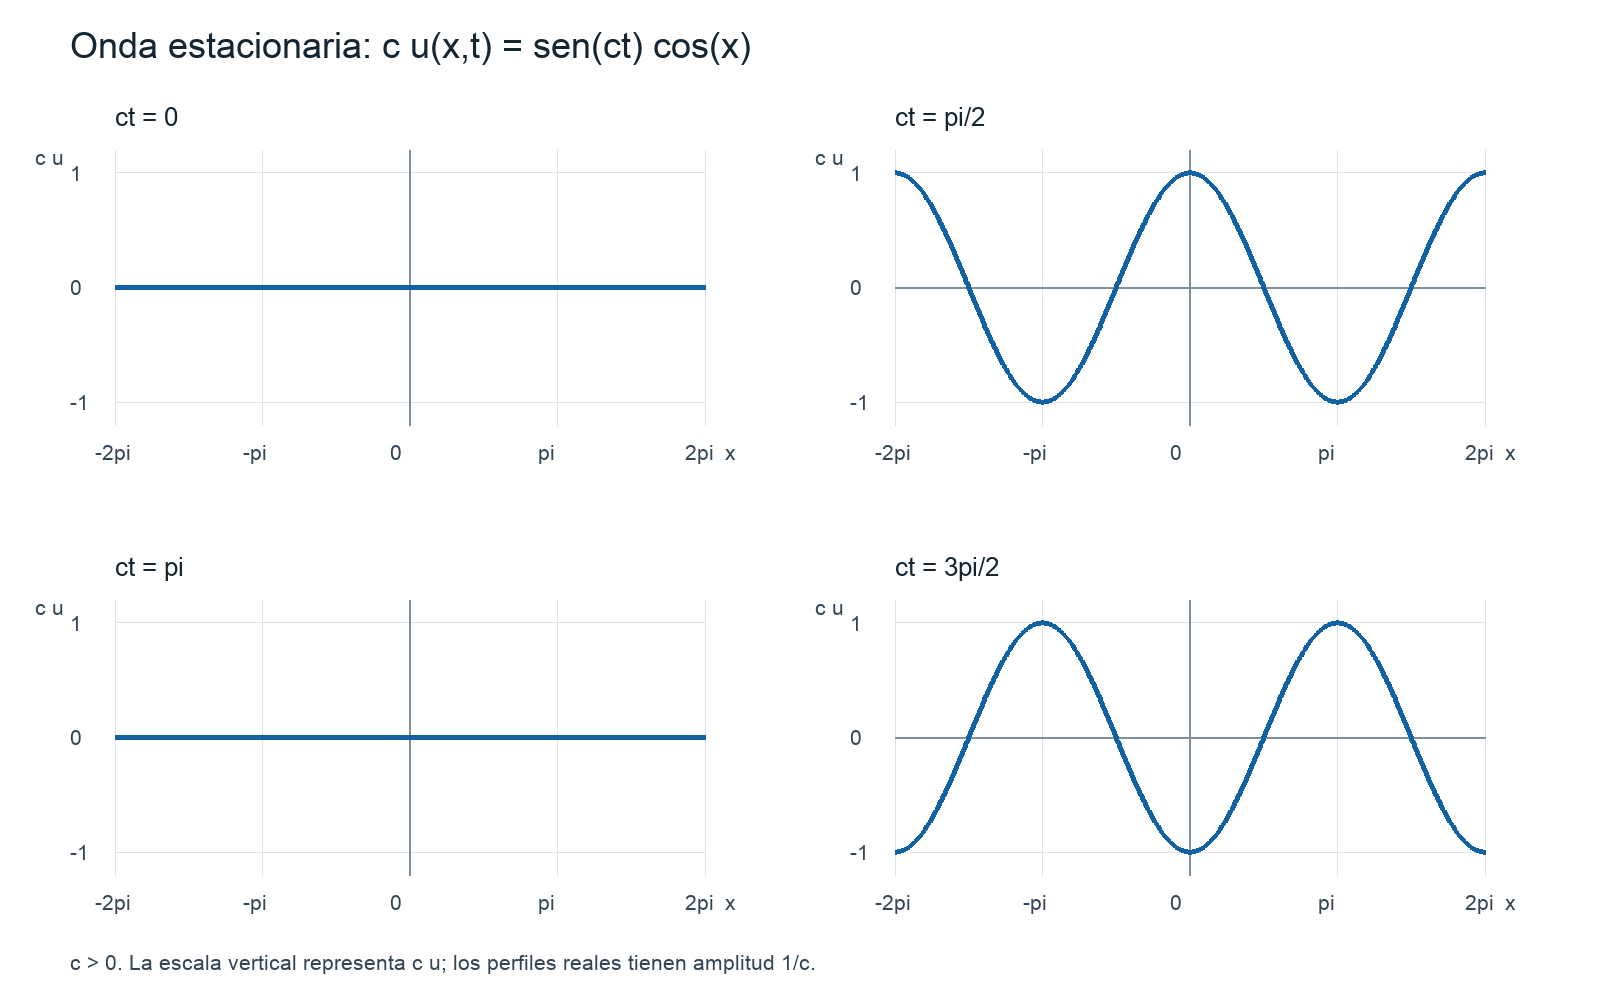
\includegraphics[width=.95\linewidth]{assets/M2-E0107-wave-profiles.png}
\end{center}

\supportheading{solution}{M2-E0355}
\noindent\textbf{Resultado.} Se tiene \(r=1/4\). En orden \(j=1,2,3\), los valores interiores, en kelvin de exceso, son
\[
(U_1^1,U_2^1,U_3^1)=(2+2\sqrt2,\ 4+2\sqrt2,\ 2+2\sqrt2),
\]
\[
(U_1^2,U_2^2,U_3^2)=\left(2+\frac{3\sqrt2}{2},\ 3+2\sqrt2,\ 2+\frac{3\sqrt2}{2}\right).
\]
En el segundo paso, los valores exactos son aproximadamente \((4.155542,\ 5.876824,\ 4.155542)\,\mathrm K\). El máximo error nodal absoluto es \(0.04839643\,\mathrm K\), en el nodo central.

\noindent\textit{Desarrollo.} El cociente de pasos es adimensional:
\[
r=\frac{(1\,\mathrm{cm^2/s})(0.25\,\mathrm s)}{(1\,\mathrm{cm})^2}=\frac14.
\]
Los datos interiores iniciales, en kelvin de exceso, son
\[
(U_1^0,U_2^0,U_3^0)=(4\sqrt2,8,4\sqrt2).
\]
El esquema toma la forma
\[
U_j^{n+1}=\frac12U_j^n+\frac14U_{j-1}^n+\frac14U_{j+1}^n.
\]
En cada paso todos los valores del segundo miembro pertenecen al mismo nivel anterior. Para el primero,
\[
U_1^1=\tfrac12(4\sqrt2)+\tfrac14(0+8)=2+2\sqrt2,
\]
\[
U_2^1=\tfrac12(8)+\tfrac14(4\sqrt2+4\sqrt2)=4+2\sqrt2,
\]
y \(U_3^1=U_1^1\) por simetría. Para el segundo, usando únicamente ese vector ya completado,
\[
U_1^2=\tfrac12(2+2\sqrt2)+\tfrac14(0+4+2\sqrt2)
=2+\frac{3\sqrt2}{2},
\]
\[
U_2^2=\tfrac12(4+2\sqrt2)+\tfrac14[2(2+2\sqrt2)]
=3+2\sqrt2,
\]
y \(U_3^2=U_1^2\). El vector aproximado final es
\[
(4.12132034,\ 5.82842712,\ 4.12132034)\,\mathrm K.
\]
En \(t=0.5\,\mathrm s\), el factor temporal exacto es \(e^{-\pi^2/32}\). Por tanto, el vector de referencia es
\[
e^{-\pi^2/32}(4\sqrt2,8,4\sqrt2)\,\mathrm K
\approx(4.15554179,\ 5.87682355,\ 4.15554179)\,\mathrm K.
\]
Los errores absolutos son aproximadamente
\[
(0.03422144,\ 0.04839643,\ 0.03422144)\,\mathrm K,
\]
por lo que el máximo solicitado es el central. El esquema atenúa este modo algo más que la solución exacta durante los dos pasos calculados.

La comparación concierne a esos nodos, ese tiempo y ese dato inicial. No establece un orden general de convergencia ni una garantía de precisión para tiempos o perfiles diferentes.

\supportheading{solution}{M2-E0109}
\noindent\textbf{(a) Resultado.} \[u(x,y)=\sum_{n=1}^{\infty}b_n\frac{\sinh(n\pi y/a)}{\sinh(n\pi b/a)}\sin\frac{n\pi x}{a},\qquad
b_n=\frac2a\int_0^a g(s)\sin\frac{n\pi s}{a}ds.\]

\noindent\textit{Desarrollo.} Separar \(u=XY\) y usar los laterales nulos da \(X_n=\sin(n\pi x/a)\),
\(Y_n''-(n\pi/a)^2Y_n=0\). La base \(y=0\) exige \(Y_n\) proporcional a \(\sinh(n\pi y/a)\).
Dividimos por \(\sinh(n\pi b/a)\) para que el factor vertical valga \(1\) en \(y=b\), y proyectamos g en senos.
Cada término es armónico y satisface los tres bordes nulos. En todo subrectángulo con \(y<b\),
los factores verticales amortiguan exponencialmente y permiten verificar la ecuación por derivación.
La regularidad supuesta y \(g(0)=g(a)=0\) permiten recuperar g continuamente en la frontera superior.
El principio del máximo aplicado a la diferencia de dos soluciones da unicidad en el rectángulo.
No se intercambian los papeles de las coordenadas: el seno impone los laterales y la hiperbólica
lleva los datos desde \(y=b\) hacia el interior.

\medskip

\noindent\textbf{(b) Resultado.} \[u(x,y)=\frac{4a}{\pi^2}\sum_{n=1}^{\infty}\frac{\sin(n\pi/2)}{n^2}
\frac{\sinh(n\pi y/a)}{\sinh(n\pi b/a)}\sin\frac{n\pi x}{a}.\]

\noindent\textit{Desarrollo.} Partimos la integral de \(b_n\) en \(a/2\) y usamos
\(\int x\sin(kx)dx=-x\cos(kx)/k+\sin(kx)/k^2\), con \(k=n\pi/a\).
Los términos de coseno se cancelan y
\[b_n=\frac{4a}{n^2\pi^2}\sin\frac{n\pi}{2}.\]
Solo aparecen índices impares con signos alternos. La suma en \(y=b\) es exactamente
la expansión seno del triángulo; en \(y=0\) o \(x=0,a\) vale cero. Como \(0\le g\le a/2\),
la solución completa satisface \(0\le u\le a/2\) por el principio del máximo. El crecimiento aparente
de \(\sinh\) en \(y\) no produce divergencia: el cociente es \(\le1\) para \(0\le y\le b\).

\supportheading{solution}{M2-E0356}
\noindent\textbf{Resultado.} El sistema es
\[
4A-B-C=23,\qquad 4B-A-D=43,
\]
\[
4C-A-D=15,\qquad 4D-B-C=35.
\]
Su solución es \((A,B,C,D)=(13,18,11,16)\). Son los valores de \(H\) en los cuatro nodos interiores. El polinomio es armónico, coincide con los datos de contorno de la tabla y sus diferencias segundas son exactas. Este acuerdo es propio de la referencia y la malla dadas; no establece error nulo en problemas generales ni determina valores de contorno entre los nodos.

\noindent\textit{Desarrollo.} Con paso uno en ambas direcciones, la suma de las dos diferencias centradas aproxima la ecuación de equilibrio por
\[
4U_{i,j}=U_{i+1,j}+U_{i-1,j}+U_{i,j+1}+U_{i,j-1}.
\]
Cada incógnita se relaciona con sus cuatro vecinos inmediatos. Para \(A\), los vecinos conocidos son \(10\) y \(13\), mientras los interiores son \(B,C\). Para \(B\), los conocidos son \(25,18\), y los interiores \(A,D\). Las otras dos filas se construyen del mismo modo:
\[
\begin{aligned}
4A&=B+C+10+13,\\
4B&=A+D+25+18,\\
4C&=A+D+8+7,\\
4D&=B+C+23+12.
\end{aligned}
\]
Restar la cuarta ecuación de la primera da \(A-D=-3\), y restar la tercera de la segunda da \(B-C=7\). Así, \(D=A+3\) y \(B=C+7\). Las ecuaciones primera y tercera se reducen a
\[
2A-C=15,\qquad 2C-A=9.
\]
De ellas se obtiene \(A=13\), \(C=11\), y después \(B=18\), \(D=16\). Estas eliminaciones reversibles también muestran la unicidad de la solución del sistema.

Para la referencia,
\[
H_{xx}=2,\qquad H_{yy}=-2,
\]
por lo que \(H\) es armónico. Sus valores en los nodos de cada lado reproducen la tabla: abajo son \(10,13,18,25\); arriba, \(4,7,12,19\); los valores intermedios izquierdos son \(10,8\), y los derechos, \(25,23\). En el interior,
\[
H(1,1)=13,\quad H(2,1)=18,\quad H(1,2)=11,\quad H(2,2)=16.
\]
El acuerdo tiene una explicación adicional al cálculo numérico: las diferencias centradas segundas reproducen exactamente la segunda derivada de un polinomio cuadrático. Aplicadas a \(H\), sus contribuciones horizontal y vertical son \(2\) y \(-2\), que se cancelan. Los valores de \(H\) satisfacen, por tanto, el mismo sistema discreto.

Los datos suministrados son valores en nodos de contorno. No fijan por sí solos una función en todos los puntos de los lados. \(H\) es una referencia armónica que interpola esos nodos; afirmar que es la única solución de un problema continuo exigiría prescribir, además, sus trazas completas en la frontera. Tampoco el acuerdo exacto de esta referencia implica que el esquema carezca de error para otros campos.

\supportheading{solution}{M2-E0268}
\noindent\textbf{Resultado.} \[u(x,t)=200\left(1-\frac x\pi\right)-\sum_{n=1}^{\infty}\frac{400}{n\pi}e^{-n^2t}\sin(nx).\]

\noindent\textit{Desarrollo.} El modelo es $u_t=u_{xx}$. El perfil estacionario que cumple los extremos es $q=200(1-x/\pi)$. La diferencia $v=u-q$ satisface la ecuación homogénea con extremos nulos y dato $v(x,0)=-q(x)$. Sus coeficientes de senos son \[b_n=-\frac2\pi\int_0^\pi200(1-x/\pi)\sin(nx)\,dx=-\frac{400}{n\pi}.\] Multiplicar cada modo por $e^{-n^2t}$ da la respuesta. Para $t>0$, la convergencia uniforme de las series derivadas verifica la EDP y las condiciones de frontera. En cada punto interior la serie inicial representa $-q$, y por tanto $u\to0$ cuando $t\downarrow0$. La esquina $(0,0)$ es incompatible: no se exige continuidad allí entre el dato interior 0 y el extremo 200. La solución tiende al perfil afín $q$ cuando $t\to\infty$.

\supportheading{solution}{M2-E0380}
\noindent\textbf{Resultado.} La malla gruesa da \(2.50000\,\mathrm K\) en el centro. Al refinar, conservar \(\Delta t=0.25\,\mathrm s\) da \(r=1\) y un modo con multiplicador de módulo mayor que uno. Para conservar \(r=1/4\), tome \(\Delta t=0.0625\,\mathrm s\); ocho pasos dan \(2.81738\,\mathrm K\). La referencia es \(2.91213\,\mathrm K\): los errores son aproximadamente \(0.41213\,\mathrm K\) y \(0.09475\,\mathrm K\). Sólo el cálculo refinado satisface la tolerancia dada.

\noindent\textit{Desarrollo.} La solución de referencia satisface los extremos, el perfil inicial y \(u_t=\kappa u_{xx}\): las dos derivadas aportan el mismo factor \(-\kappa\pi^2/L^2\). En el centro \(\sin(\pi/2)=1\), de modo que
\[
u(L/2,T)=10e^{-\pi^2/8}\,\mathrm K\simeq2.912129332\,\mathrm K.
\]

En la malla gruesa r=1/4. Hay un solo nodo interior y sus vecinos son extremos nulos, así que cada paso multiplica por \(1-2r=1/2\). Dos pasos hasta T dan \(10(1/2)^2=2.5\,\mathrm K\). El error absoluto es \(0.412129332\,\mathrm K\), aunque el paso cumple el criterio de estabilidad suministrado.

Al dividir \(\Delta x\) por dos y conservar \(\Delta t\), r se multiplica por cuatro: sería uno. La pérdida de una condición suficiente por sí sola no demostraría inestabilidad, pero aquí se puede comprobar un modo concreto. Para la malla fina, \(\Delta x=0.5\) y \(m=3\),
\[
g_3=1-4\sin^2(3\pi/8)=-1-\sqrt2,
\]
con módulo mayor que uno. Una perturbación de ese modo crece. El perfil inicial exacto es sólo el modo m=1, para el que \(g_1=\sqrt2-1\) con r=1: observar únicamente ese modo ocultaría la inestabilidad frente a otras perturbaciones admisibles.

Para conservar r=1/4, se divide \(\Delta t\) por cuatro: \(0.0625\,\mathrm s\). Se necesitan ocho pasos. La identidad
\(\sin(a-b)+\sin(a+b)=2\sin a\cos b\)
comprueba el multiplicador dado al introducir un modo en el esquema. Para m=1,
\[
g_1=1-\sin^2(\pi/8)=\frac{2+\sqrt2}{4}.
\]
En el centro el modo vale uno, por lo que la respuesta refinada es
\[
10\left(\frac{2+\sqrt2}{4}\right)^8\,\mathrm K
\simeq2.817380697\,\mathrm K.
\]
Su error \(0.094748635\,\mathrm K\) es menor que \(0.10\,\mathrm K\). La malla fina supera el requisito estipulado; la gruesa no. Se han comparado el mismo punto y el mismo tiempo final, con precisión numérica suficiente para decidir una tolerancia próxima.

La estabilidad controla crecimiento de perturbaciones, no el tamaño del error de discretización. Refinar sólo el tiempo mantiene un error espacial que no tiene por qué cumplir el requisito. Esta comparación de un modo y dos mallas tampoco demuestra un orden general de convergencia para cualquier dato inicial.

\supportheading{solution}{M2-E0357}
\noindent\textbf{Resultado.} Si \(a=\kappa\pi^2/L^2\), el problema transformado es
\[
\kappa U_{xx}-sU=-\Theta\left[3\sin(\pi x/L)-\sin(2\pi x/L)\right],
\qquad U(0,s)=U(L,s)=0.
\]
Para cada \(s>0\), su solución única es
\[
U(x,s)=\frac{3\Theta}{s+a}\sin(\pi x/L)
-\frac{\Theta}{s+4a}\sin(2\pi x/L).
\]
La inversión da
\[
u(x,t)=3\Theta e^{-at}\sin(\pi x/L)
-\Theta e^{-4at}\sin(2\pi x/L).
\]
Esta función satisface la EDP y todos los datos; sus transformadas y las de las derivadas utilizadas existen para \(s>0\).

\noindent\textit{Desarrollo.} Denotemos el perfil inicial por
\[
f(x)=\Theta[3\sin(\pi x/L)-\sin(2\pi x/L)].
\]
Al transformar la EDP respecto del tiempo, la derivada temporal produce el término inicial:
\[
\mathcal L_t[u_t]=sU(x,s)-f(x).
\]
Bajo el intercambio de operaciones permitido, \(\mathcal L_t[u_{xx}]=U_{xx}\). Por tanto,
\[
sU-f=\kappa U_{xx}.
\]
Las funciones de contorno son cero para todo tiempo positivo, así que sus transformadas también son cero. El problema espacial que hay que resolver es
\[
\kappa U_{xx}-sU=-f(x),\qquad U(0,s)=U(L,s)=0.
\]
Se ha transformado la ecuación distribuida y sus datos, conservando el campo inicial como término de la EDO espacial.

Sea \(a=\kappa\pi^2/L^2\). Buscamos una solución particular de esa EDO como combinación de los dos senos presentes en \(f\). Al sustituir
\[
U_p=A\sin(\pi x/L)+B\sin(2\pi x/L),
\]
se obtiene
\[
-(s+a)A=-3\Theta,\qquad -(s+4a)B=\Theta.
\]
Así,
\[
U_p=\frac{3\Theta}{s+a}\sin(\pi x/L)
-\frac{\Theta}{s+4a}\sin(2\pi x/L),
\]
que ya cumple ambos contornos. Los denominadores son positivos para \(s>0\).

Para justificar la unicidad, la diferencia \(W\) entre dos soluciones cumpliría \(\kappa W''-sW=0\) y \(W(0)=W(L)=0\). Multiplicando por \(W\), integrando y usando los contornos,
\[
0=\int_0^L W(\kappa W''-sW)\,dx
=-\kappa\int_0^L(W')^2\,dx-s\int_0^L W^2\,dx.
\]
Como \(\kappa,s>0\), necesariamente \(W=0\). Por tanto, \(U=U_p\) es la única solución del problema transformado.

La pareja elemental \(\mathcal L^{-1}[1/(s+b)]=e^{-bt}\), para \(b>0\), proporciona
\[
u(x,t)=3\Theta e^{-at}\sin(\pi x/L)
-\Theta e^{-4at}\sin(2\pi x/L).
\]
Cada derivada temporal multiplica el primer término por \(-a\) y el segundo por \(-4a\); \(\kappa\) veces sus segundas derivadas espaciales introduce esos mismos factores. Se verifica así la EDP. Ambos senos se anulan en los extremos, y al poner \(t=0\) se recupera exactamente \(f(x)\).

Finalmente, la función y las derivadas utilizadas son sumas finitas de senos o cosenos multiplicados por exponenciales decrecientes. En todo \([0,L]\) están acotadas por una constante multiplicada por \(e^{-at}\). Para cualquier \(s>0\), sus integrales contra \(e^{-st}\) convergen; esa misma cota permite intercambiar la integración y las derivadas espaciales de esta función. El término temporal de borde en infinito también se anula. El parámetro \(a\), como \(s\), tiene unidades de tiempo inverso, y \(U\) tiene unidades de temperatura multiplicada por tiempo.

\chapter{Apoyo para las mallas largas}
En los ejercicios \exref{M2-E0049} y \exref{M2-E0068}, las mallas largas pueden calcularse con una hoja de cálculo o con el programa opcional \href{https://github.com/gioda/ecuaciones-diferenciales/blob/main/scripts/mallas.py}{\texttt{scripts/mallas.py}}, que usa Python 3 sin paquetes adicionales. El programa escribe tablas de valores; no hace falta desarrollar a mano todas las actualizaciones. Conviene comprobar primero una de ellas y conservar todos los decimales durante el cálculo.

Para un sistema \(Y'=F(t,Y)\), Euler explícito utiliza
\[
Y_{n+1}=Y_n+hF(t_n,Y_n).
\]
El esquema clásico de Runge--Kutta de cuarto orden, con pendientes sin incluir el paso, es
\[
\begin{aligned}
K_1&=F(t_n,Y_n),\\
K_2&=F(t_n+h/2,Y_n+hK_1/2),\\
K_3&=F(t_n+h/2,Y_n+hK_2/2),\\
K_4&=F(t_n+h,Y_n+hK_3),\\
Y_{n+1}&=Y_n+\frac h6(K_1+2K_2+2K_3+K_4).
\end{aligned}
\]
Cada etapa usa un vector completo: no se mezcla una componente ya actualizada con otra del paso anterior.

Desde la carpeta de fuentes del libro, las órdenes son:
\begin{verbatim}
python3 scripts/mallas.py E0049
python3 scripts/mallas.py E0068
\end{verbatim}
La primera produce 40 pasos con \(h=0.025\). La segunda genera las tres mallas pedidas hasta \(t=2\); para representar \(y\), se utilizan las columnas \texttt{t} e \texttt{y} de cada malla. La comparación entre pasos informa del efecto del refinamiento, pero por sí sola no certifica una cota del error respecto de la solución exacta.

\chapter{Índice de consulta}
Tasas, soluciones y datos iniciales: capítulo 1, pág.\ \pageref{CH01-B01}.\par
Separación, equilibrios y dominio: capítulo 1, pág.\ \pageref{CH01-B02}.\par
Campos, unicidad y prolongación: capítulo 1, pág.\ \pageref{CH01-B03}.\par
Balances y dominio físico: capítulo 1, pág.\ \pageref{CH01-B04}.\par
Linealidad y respuesta integral: capítulo 2, pág.\ \pageref{CH02-B01}.\par
Exactitud, potenciales y factores: capítulo 2, pág.\ \pageref{CH02-B02}.\par
Sustituciones y equivalencia: capítulo 2, pág.\ \pageref{CH02-B03}.\par
Balances, parámetros y cambios de operación: capítulo 2, pág.\ \pageref{CH02-B04}.\par
Actualizaciones y comparación de resultados: capítulo 3, pág.\ \pageref{CH03-B01}.\par
Error y garantías del paso: capítulo 3, pág.\ \pageref{CH03-B02}.\par
Calibración, observación y contraste: capítulo 3, pág.\ \pageref{CH03-B03}.\par
Respuesta integral y comparación de entradas: capítulo 3, pág.\ \pageref{CH03-B04}.\par
Estructura y condiciones: capítulo 4, pág.\ \pageref{CH04-B01}.\par
Raíces y bases reales: capítulo 4, pág.\ \pageref{CH04-B02}.\par
Reducción y dominio: capítulo 4, pág.\ \pageref{CH04-B03}.\par
Particulares y elección de vía: capítulo 4, pág.\ \pageref{CH04-B04}.\par
Modelos, recuperación de datos y comparación: capítulo 4, pág.\ \pageref{CH04-B05}.\par
Variables, equilibrio y unidades: capítulo 5, pág.\ \pageref{CH05-B01}.\par
Regímenes y lectura de la respuesta: capítulo 5, pág.\ \pageref{CH05-B02}.\par
Forzamiento y resonancia: capítulo 5, pág.\ \pageref{CH05-B03}.\par
Identificación y alcance del modelo: capítulo 5, pág.\ \pageref{CH05-B04}.\par
Definición y existencia: capítulo 6, pág.\ \pageref{CH06-B01}.\par
Relojes y propiedades: capítulo 6, pág.\ \pageref{CH06-B02}.\par
Transformación del PVI e inversión: capítulo 6, pág.\ \pageref{CH06-B03}.\par
Eventos, continuidad y decisión: capítulo 6, pág.\ \pageref{CH06-B04}.\par
Estados y equivalencia: capítulo 7, pág.\ \pageref{CH07-B01}.\par
Evolución lineal: capítulo 7, pág.\ \pageref{CH07-B02}.\par
Balances y observación: capítulo 7, pág.\ \pageref{CH07-B03}.\par
Avance vectorial y límites de la comparación: capítulo 7, pág.\ \pageref{CH07-B04}.\par
Simetría y producto escalar: capítulo 8, pág.\ \pageref{CH08-B01}.\par
Coeficientes y elección de extensión: capítulo 8, pág.\ \pageref{CH08-B02}.\par
Suma, empalmes y perfiles: capítulo 8, pág.\ \pageref{CH08-B03}.\par
Proyección y alcance del error: capítulo 8, pág.\ \pageref{CH08-B04}.\par
Problema regular y casos del parámetro: capítulo 9, pág.\ \pageref{CH09-B01}.\par
Normalización y expansión: capítulo 9, pág.\ \pageref{CH09-B02}.\par
Contornos físicos y cambio de medida: capítulo 9, pág.\ \pageref{CH09-B03}.\par
Forzamiento, compatibilidad y límites: capítulo 9, pág.\ \pageref{CH09-B04}.\par
Dos variables y datos: capítulo 10, pág.\ \pageref{CH10-B01}.\par
Modos y perfiles de evolución: capítulo 10, pág.\ \pageref{CH10-B02}.\par
Equilibrio y contornos no homogéneos: capítulo 10, pág.\ \pageref{CH10-B03}.\par
Mallas pequeñas y garantías: capítulo 10, pág.\ \pageref{CH10-B04}.\par
Laplace temporal en una EDP: capítulo 10, pág.\ \pageref{CH10-B05}.\par
